% \documentclass[12pt,endfloats]{article}%

\documentclass[endfloats,nofootinbib,preprint,floatfix,titlepage,superscriptaddress]{revtex4} %  ,endfloats,floatfix
%\documentclass[12pt,a4paper,final]{iopart}
% \documentclass[nofootinbib,floatfix,reprint,prl,endfloats,superscriptaddress]{revtex4} %  ,floatfix
%\usepackage{natbib}

\usepackage[utf8]{inputenc}
\usepackage{nima,graphicx,amsmath,amssymb,color}%,hyperref}
\usepackage{mathrsfs}
%\usepackage{graphicx}
\usepackage{comment}
% \newcommand{\Ls}{\mathscr{L}}

\usepackage{setspace}
\linespread{1.5}

\newcommand{\lrto}{\leftrightarrow}
\marginparwidth 0pt
\oddsidemargin  0pt
\evensidemargin  0pt
\marginparsep 0pt
\topmargin   -0.25in 
\textwidth   6.5in
\textheight  9.0in
\newcommand{\RNum}[1]{\uppercase\expandafter{\romannumeral #1\relax}}
\newcommand{\outNim}[1]{}
%
% \documentclass{article}
\usepackage{array}

\newcommand{\finV}[2]{#1}
% \newcommand{\finV}[2]{#2}

\begin{document}


\author{Nima Dehmamy\thanks{nidami@gmail.com}}
\affiliation{Center for Complex Network Research, Northeastern University, Boston, USA}
\author{Soodabeh Milanlouei}
\affiliation{Center for Complex Network Research, Northeastern University, Boston, USA}
\author{Albert-L\'aszl\'o Barab\'asi}
\affiliation{Center for Complex Network Research, Northeastern University, Boston, USA}
\affiliation{Center for Cancer Systems Biology, Dana Farber Cancer Institute, Boston, USA}
\affiliation{Department of Medicine, Brigham and Women’s Hospital, Harvard Medical School, Boston, USA}
\affiliation{Center for Network Science, Central European University, Budapest, Hungary}
%\maketitle
\date{\today}
% \maketitle
%\centerline{\Huge Phases of Physical 3D Networks}


\linespread{1.2}
\title{\Large Structural Phase Transition in Physical Networks}
\outNim{
\medskip
\centerline{Nima Dehmamy\footnote{nidami@gmail.com}, Soodabeh Milanlouei, Albert-L\'aszl\'o Barab\'asi}
\centerline{\today}
\bigskip
}

\finV{
  \begin{abstract}
% \begin{document}
{\bf 
In many physical networks, from neurons in the brain \cite{kasthuri12015saturated,oh2014mesoscale} to 3D integrated circuits \cite{wong2007monolithic} %,shulaker2014monolithic} %to bundles of cables carrying power in infrastructural systems 
or underground hyphal networks %\cite{friese1991spread,bago1998architecture}
\cite{friese1991spread}, the nodes and links are physical objects unable to cross each other.
These non-crossing conditions constrain their layout geometry and affect how these networks form, evolve and function, limitations ignored by the  
%Despite the recent development of 
extensive theoretical framework used to characterize real networks \cite{barrat2008dynamical,caldarelli2012networks,cohen2010complex,dorogovtsev2013evolution}. %none of the currently used network models take into account this physicality. 
Indeed, the currently used network layout methods are variants of the Force-Directed Layout (FDL) algorithm \cite{kamada1989algorithm,fruchterman1991graph}, %\cite{kamada1989algorithm,davidson1996drawing,fruchterman1991graph,barnes1986hierarchical}, 
which assumes dimensionless nodes and links, hence are inherently unable to reveal the geometry of densely packed physical networks.
Here, we develop a modeling framework inspired by manifold dynamics that accounts for the physical reality of nodes and links, allowing us to 
explore how the non-crossing conditions affect the geometry of the network layout. 
For small link thicknesses, $r_L$, we observe a weakly interacting phase where the layout avoids the numerous potential link crossings via local link rearrangements, without altering the overall layout geometry. 
Once $r_L$ exceeds a critical threshold, a strongly interacting phase emerges, where multiple geometric quantities, from the total link length to the link curvature, scale with $r_L$. 
We show that the observed transition is driven by excluded volume interactions, allowing us to analytically derive the transition point.
We also find that networks display a solid-like response to stress in the weakly interacting phase,  whereas they behave in a gel-like fashion in the strongly interacting phase, illustrating the impact of the observed transition on the physical properties of the network. 
Overall, we 
observe a deep universality, finding that the observed scaling properties are independent of the underlying network topology. 
Finally, we show that the weakly interacting phase offers avenues to 3D print networks, while the strongly interacting phase offers insight on the scaling of densely packed mammalian brains.

} 
\end{abstract}
\maketitle}{}

\linespread{1.5}

%\newpage
\begin{figure}
    \centering
    % 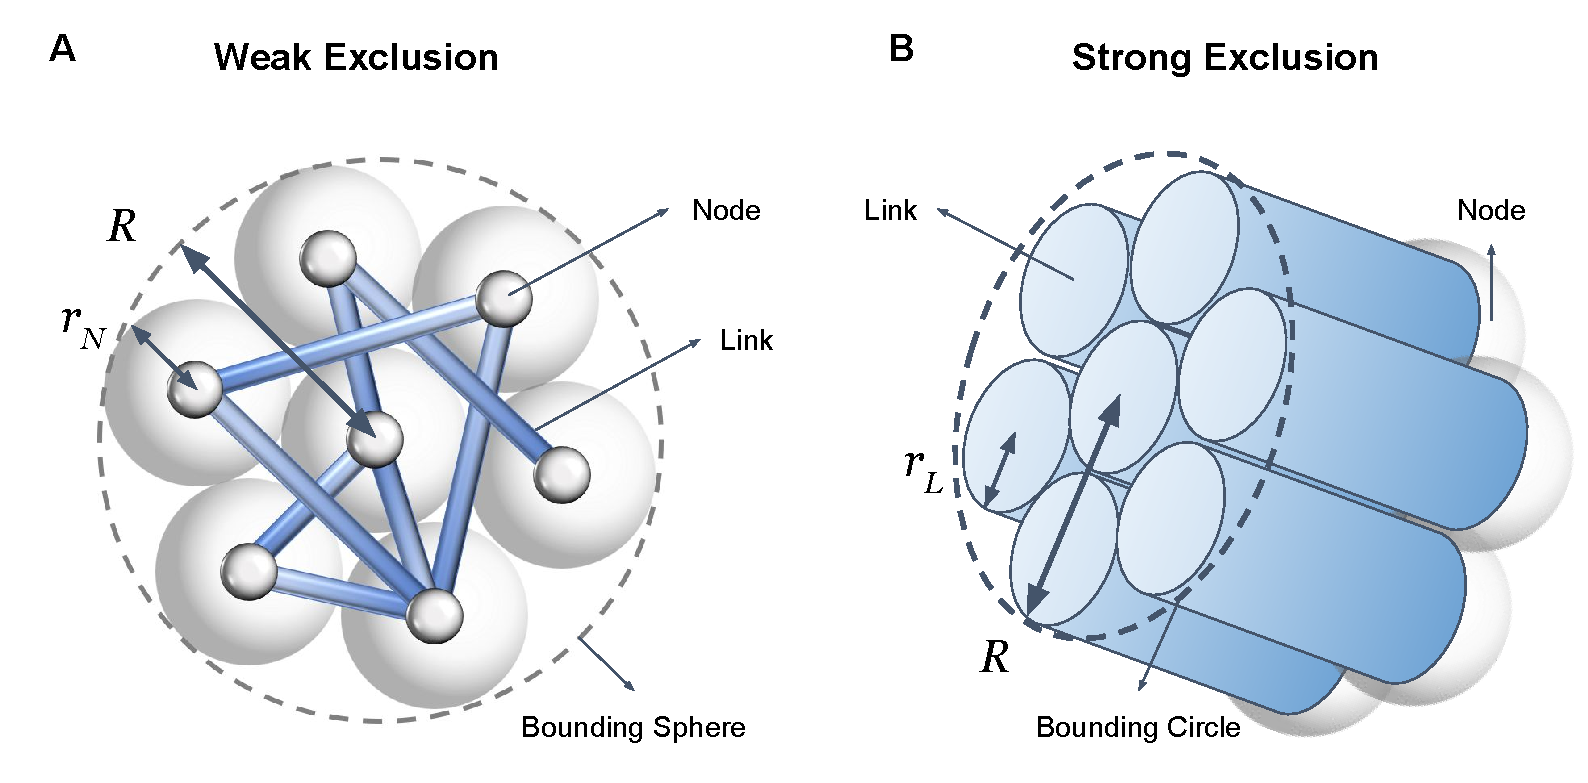
\includegraphics[width=\columnwidth]{fig-09-19/transition.pdf}
    %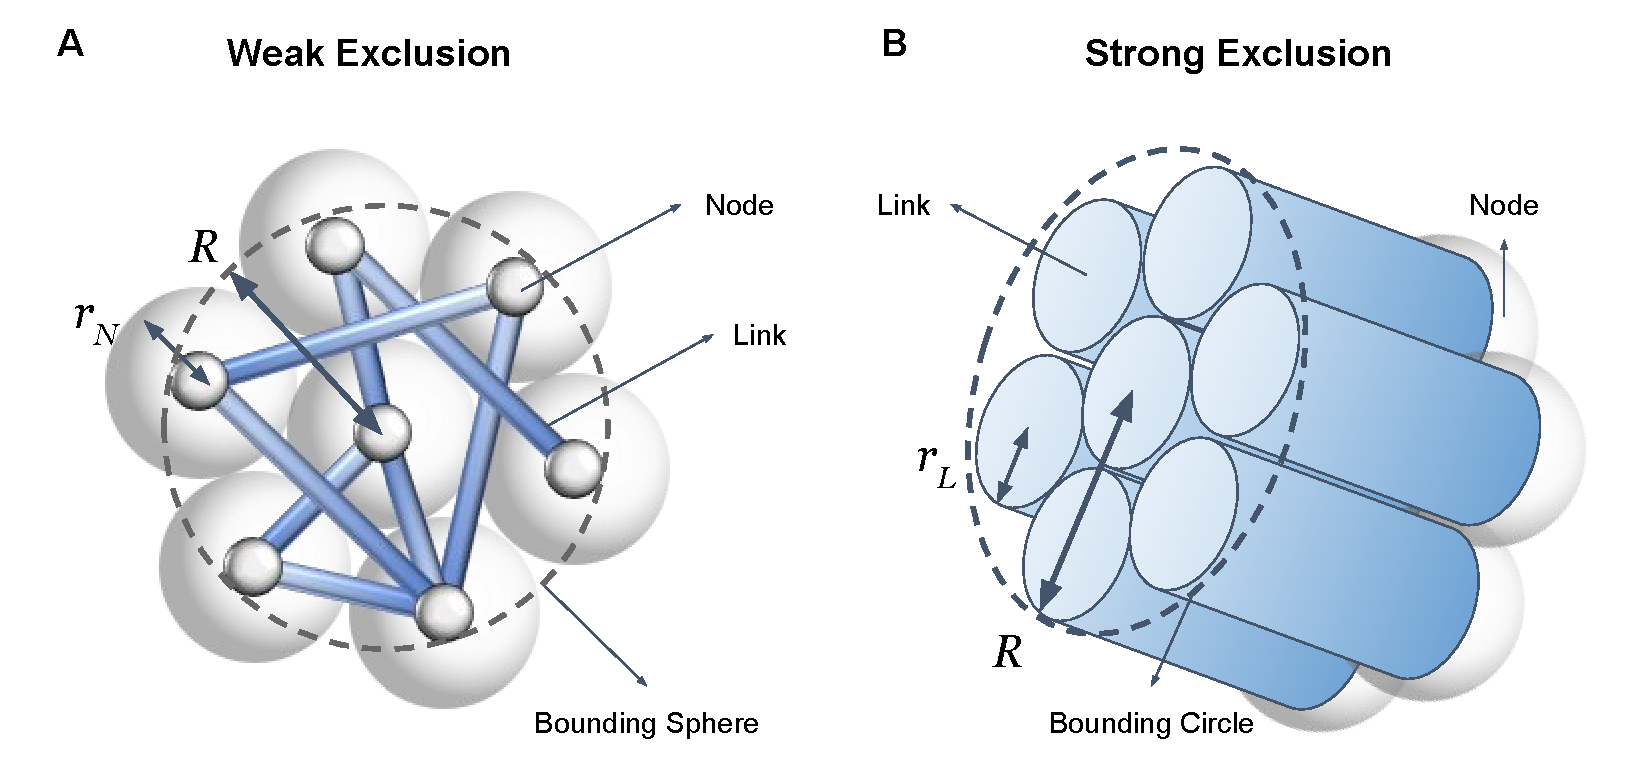
\includegraphics[width=\columnwidth]{fig-09-19/trans-2.pdf}
    %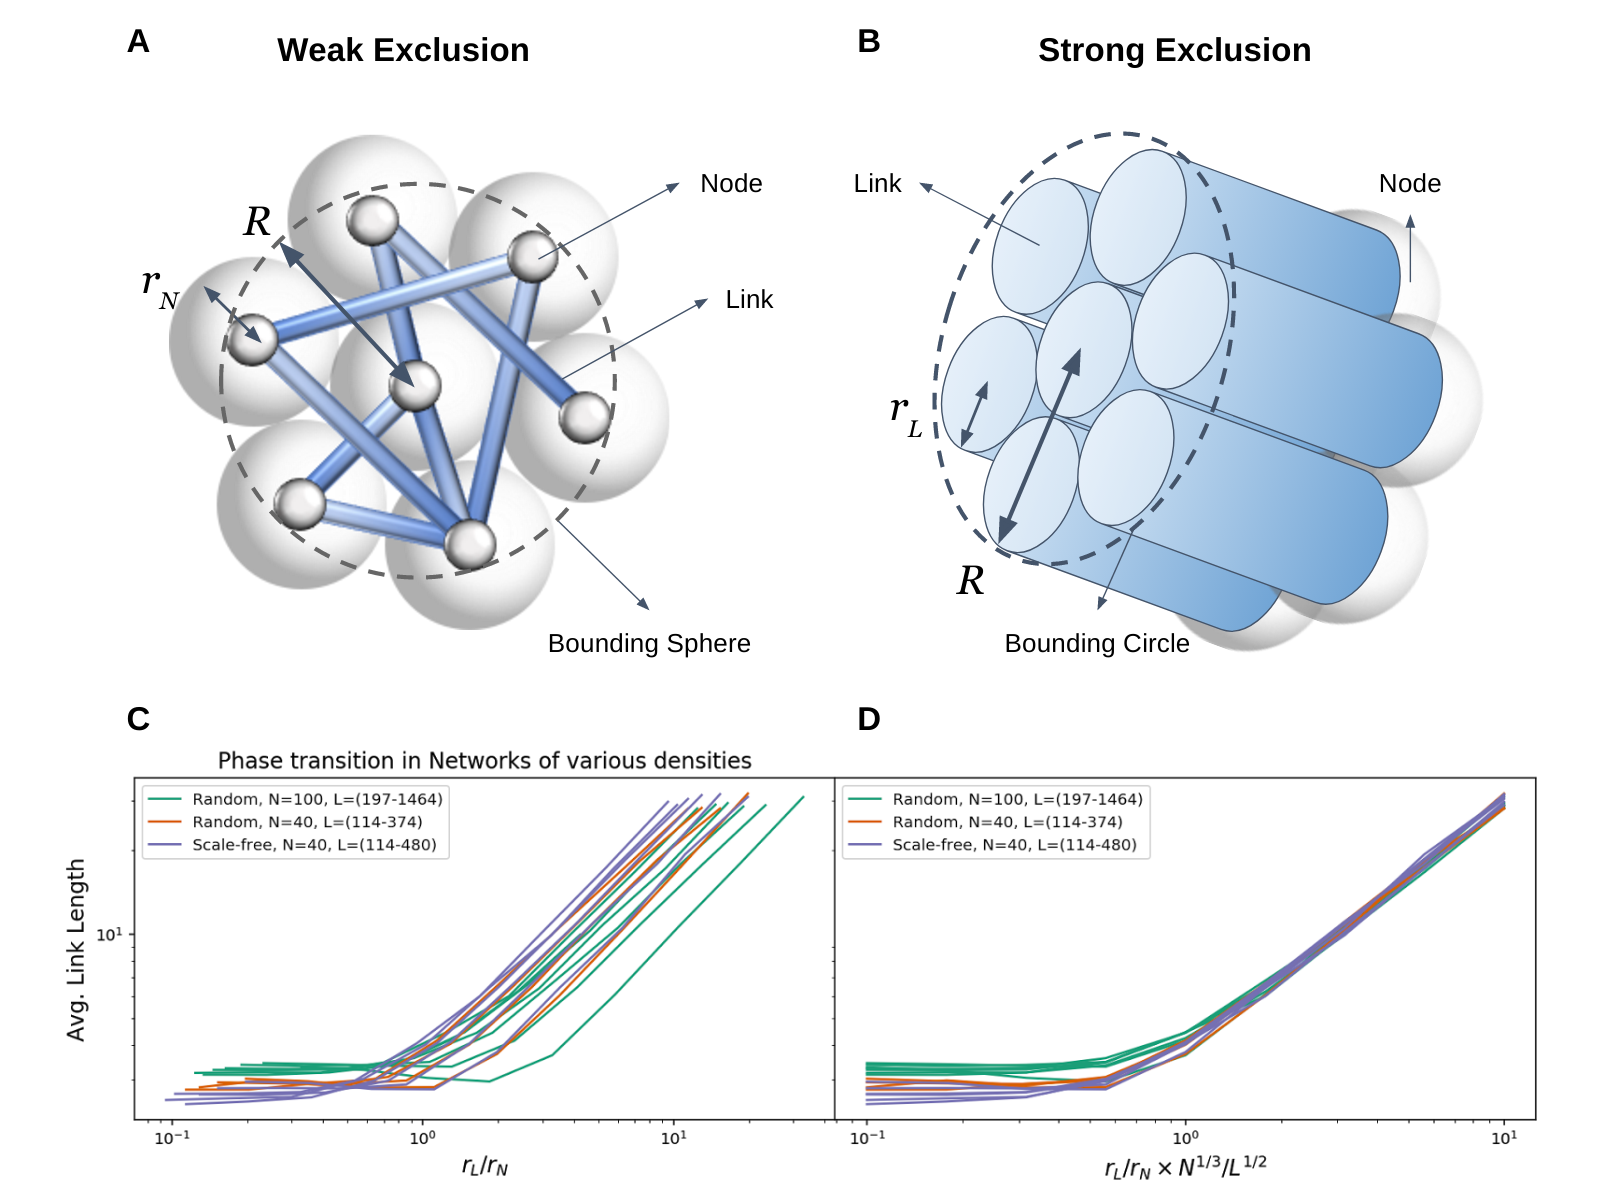
\includegraphics[width=\columnwidth]{fig-09-19/transition-2.png}
    % 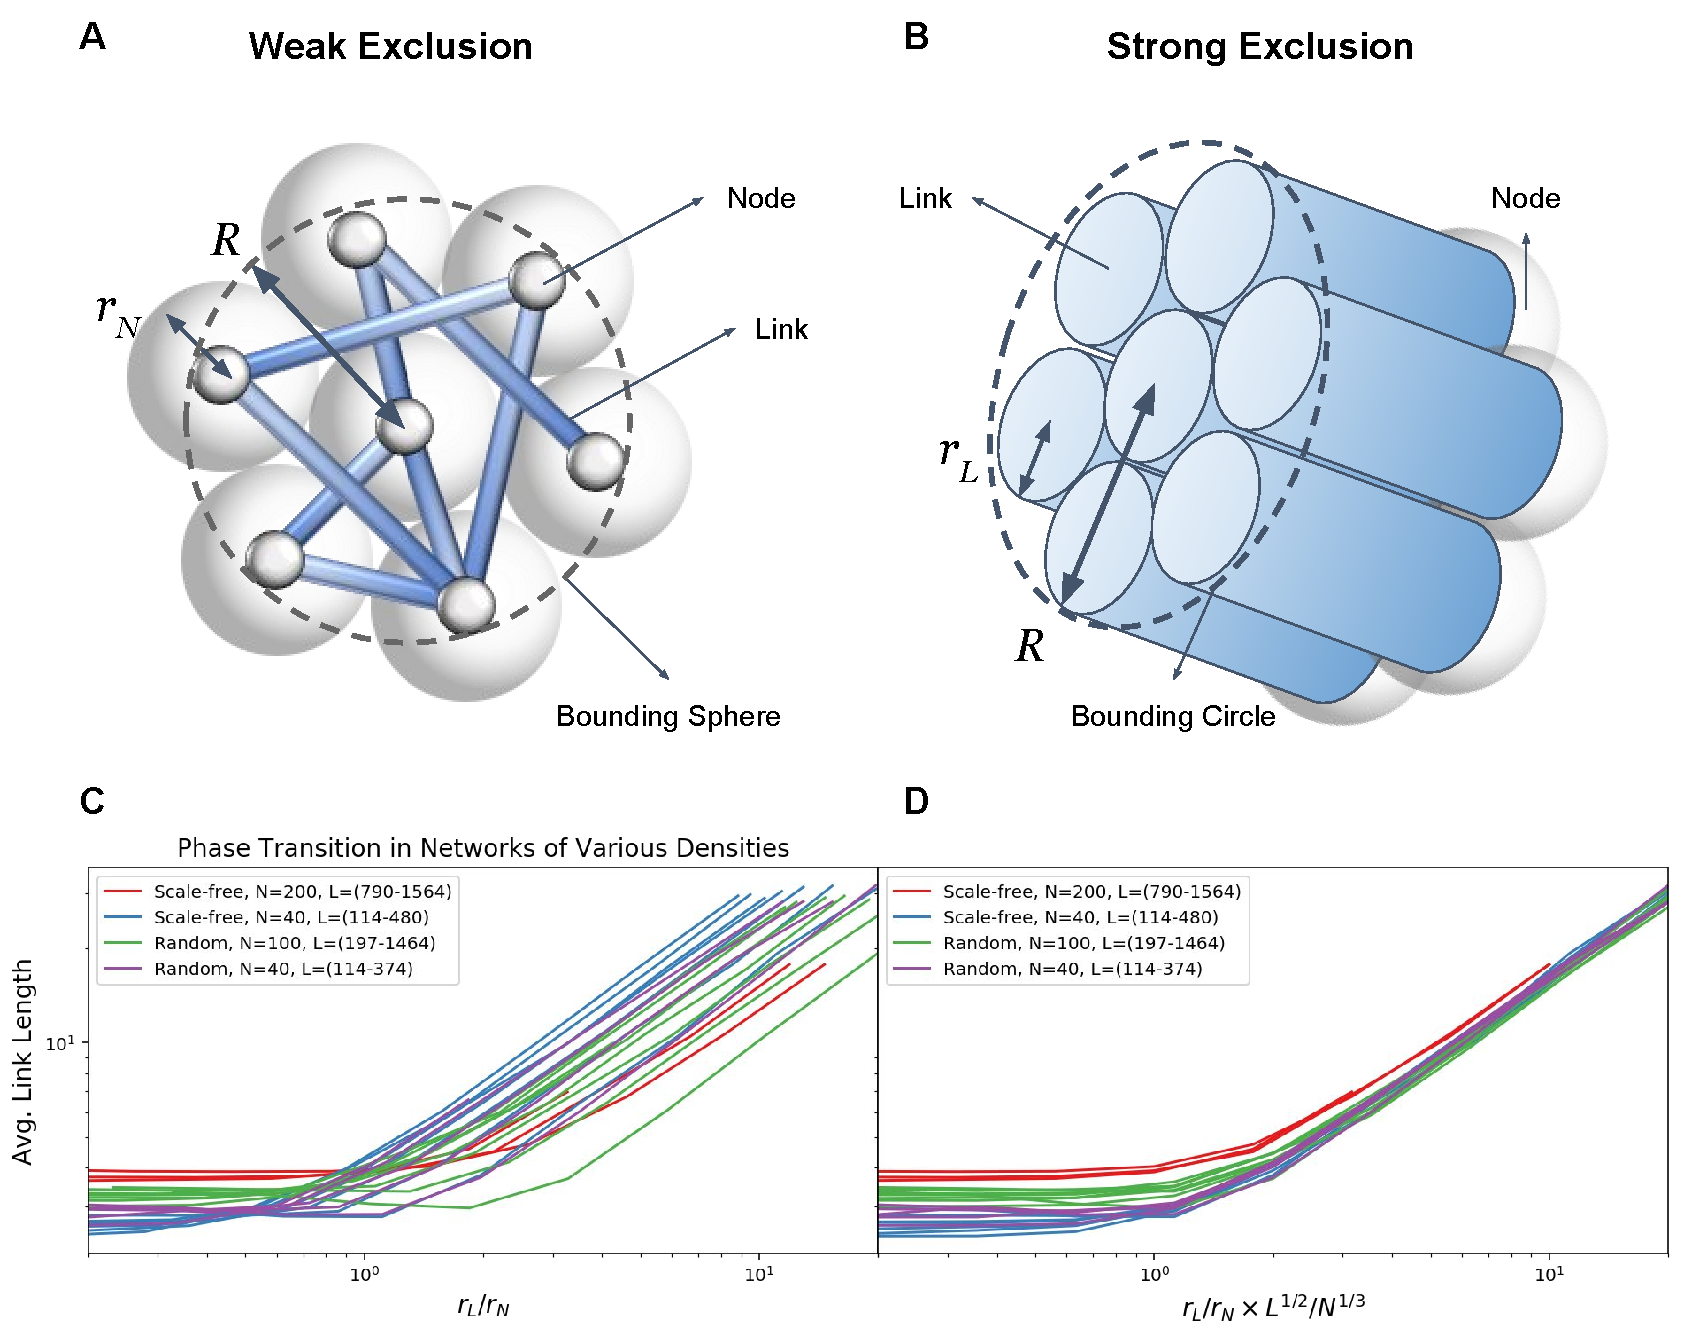
\includegraphics[width=\columnwidth]{fig-09-19/transition-3.pdf}
    % 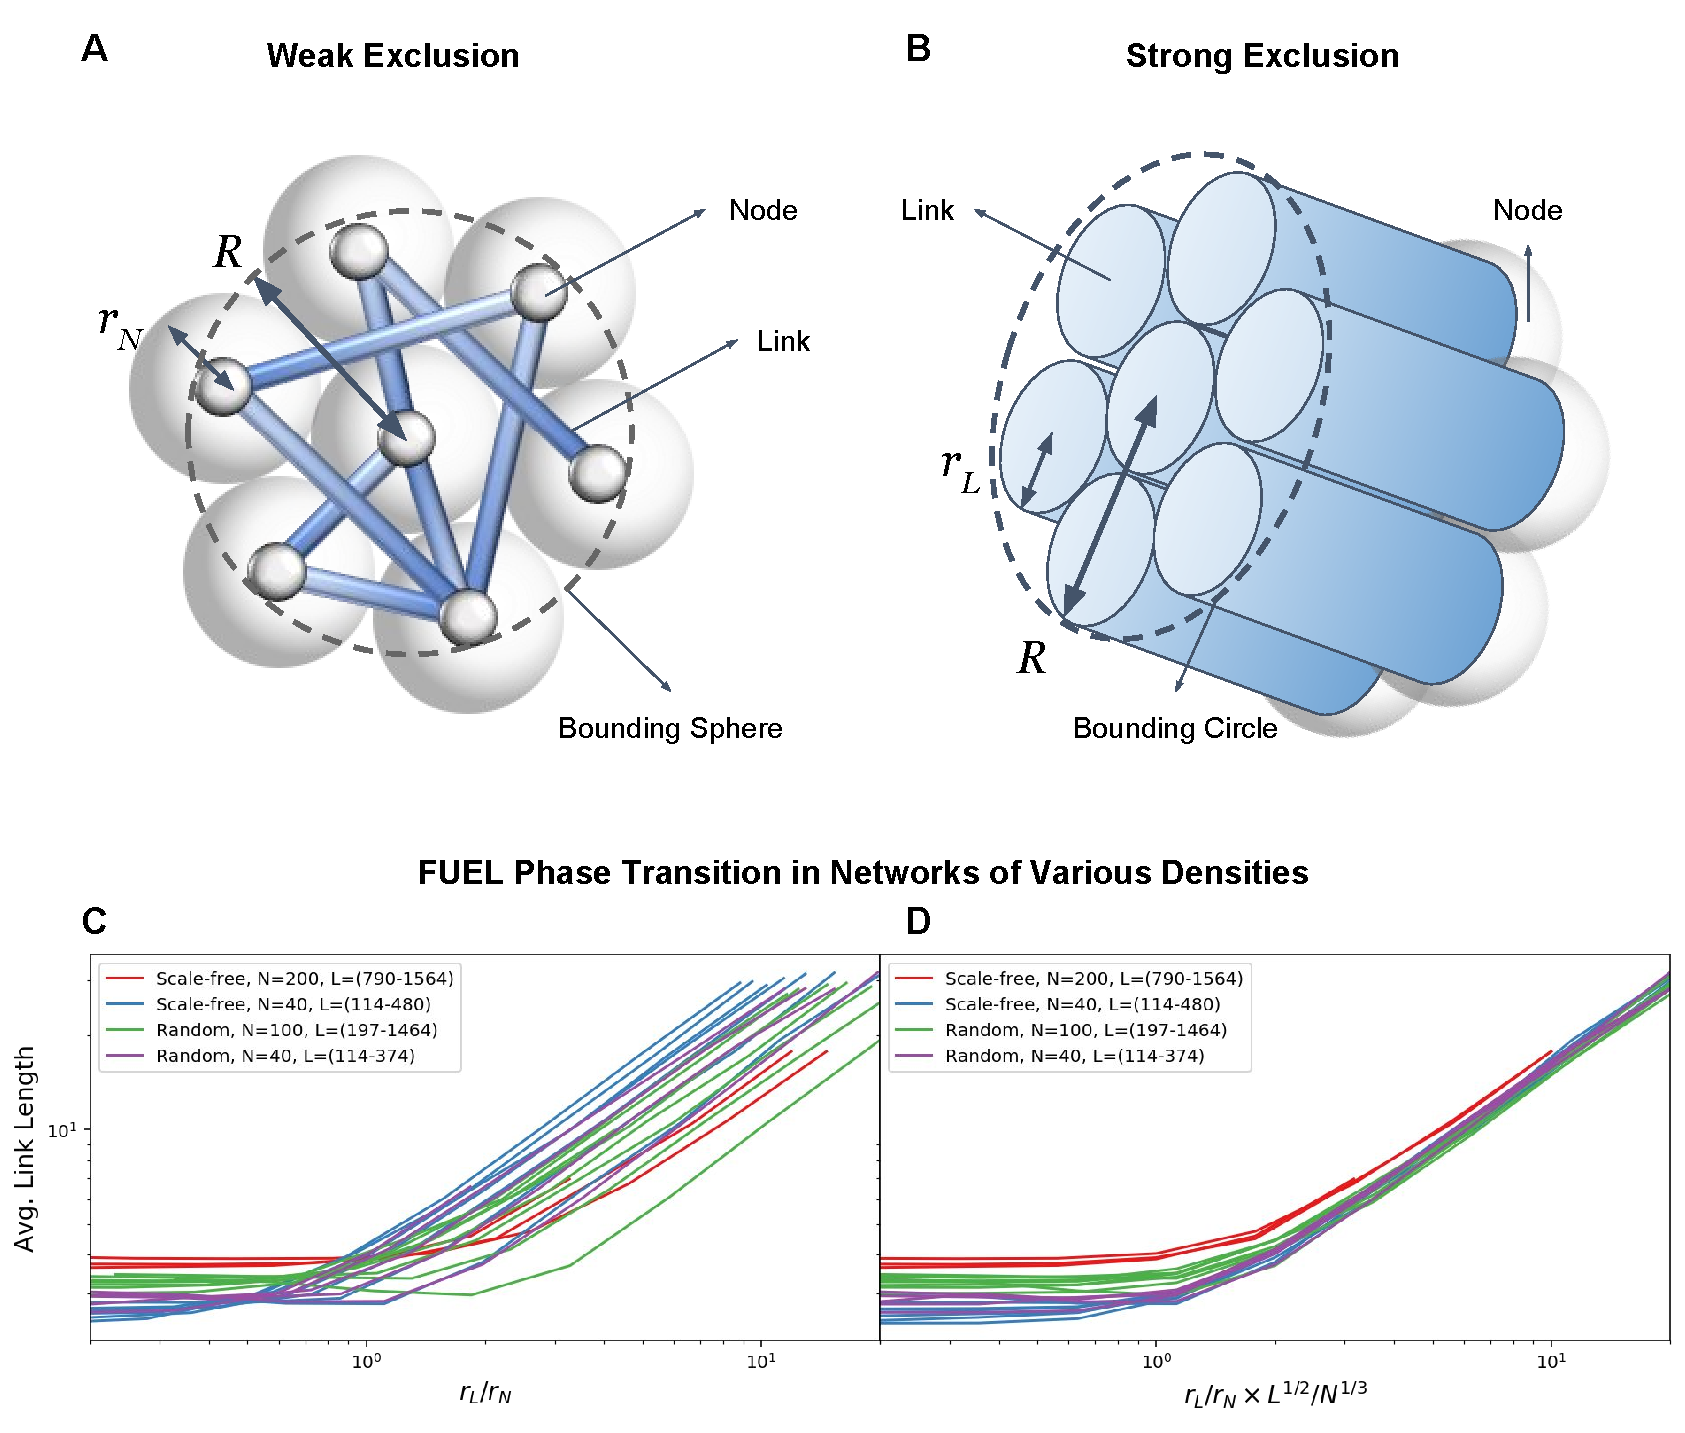
\includegraphics[width=\columnwidth]{fig-09-19/3D-transition.pdf}
    %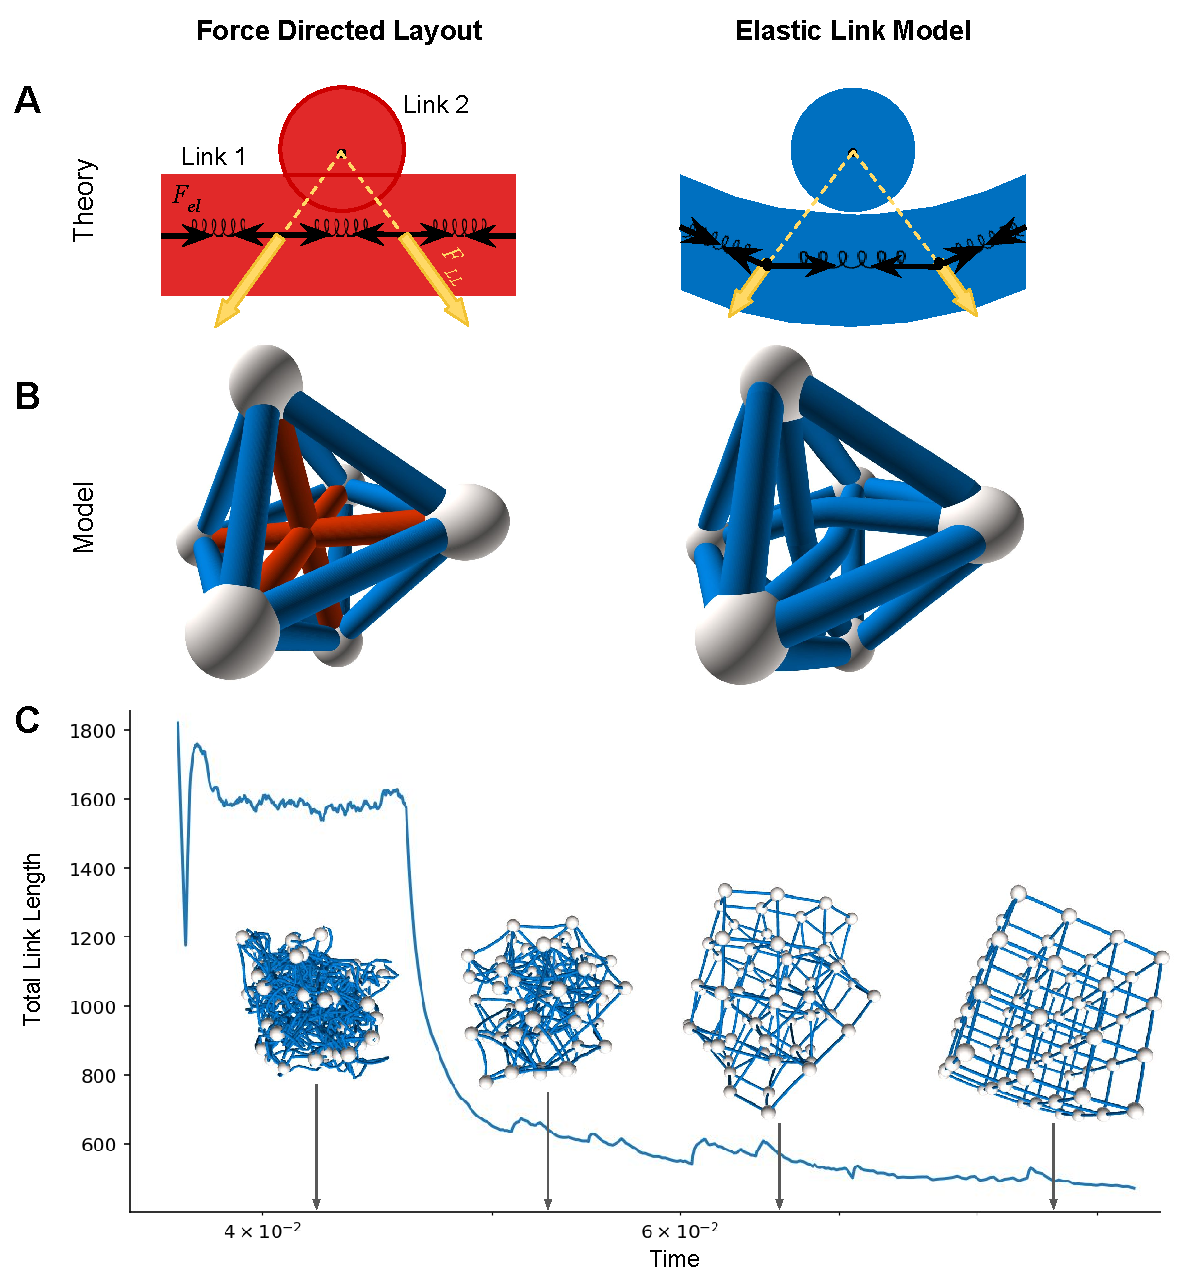
\includegraphics[width=.7\columnwidth]{fig-09-19/3D-ELM-growth.pdf}
    %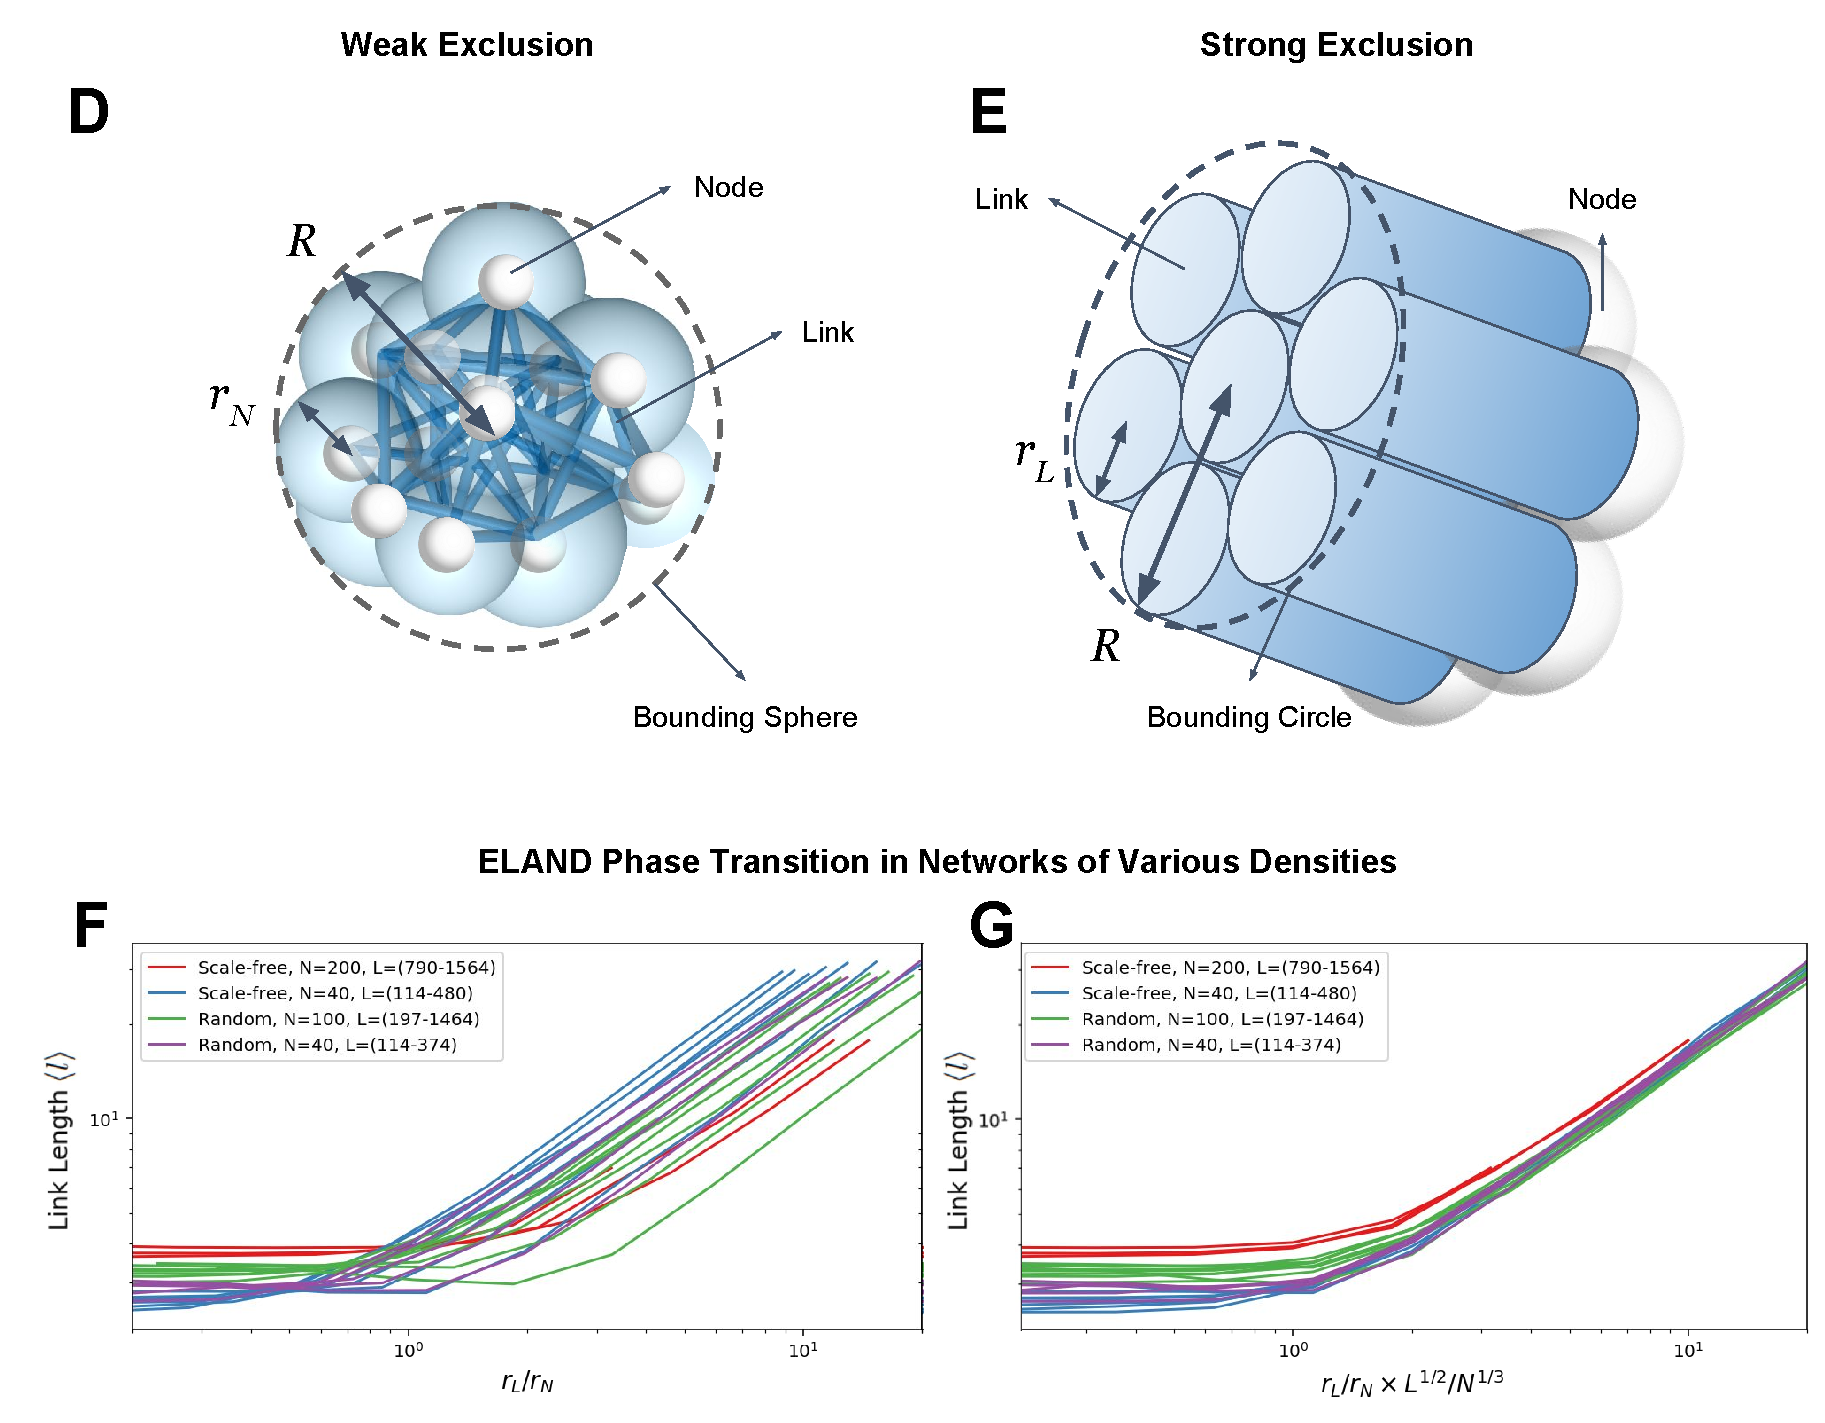
\includegraphics[width=.7\columnwidth]{fig-09-19/3D-trans-092517-1.pdf}
    %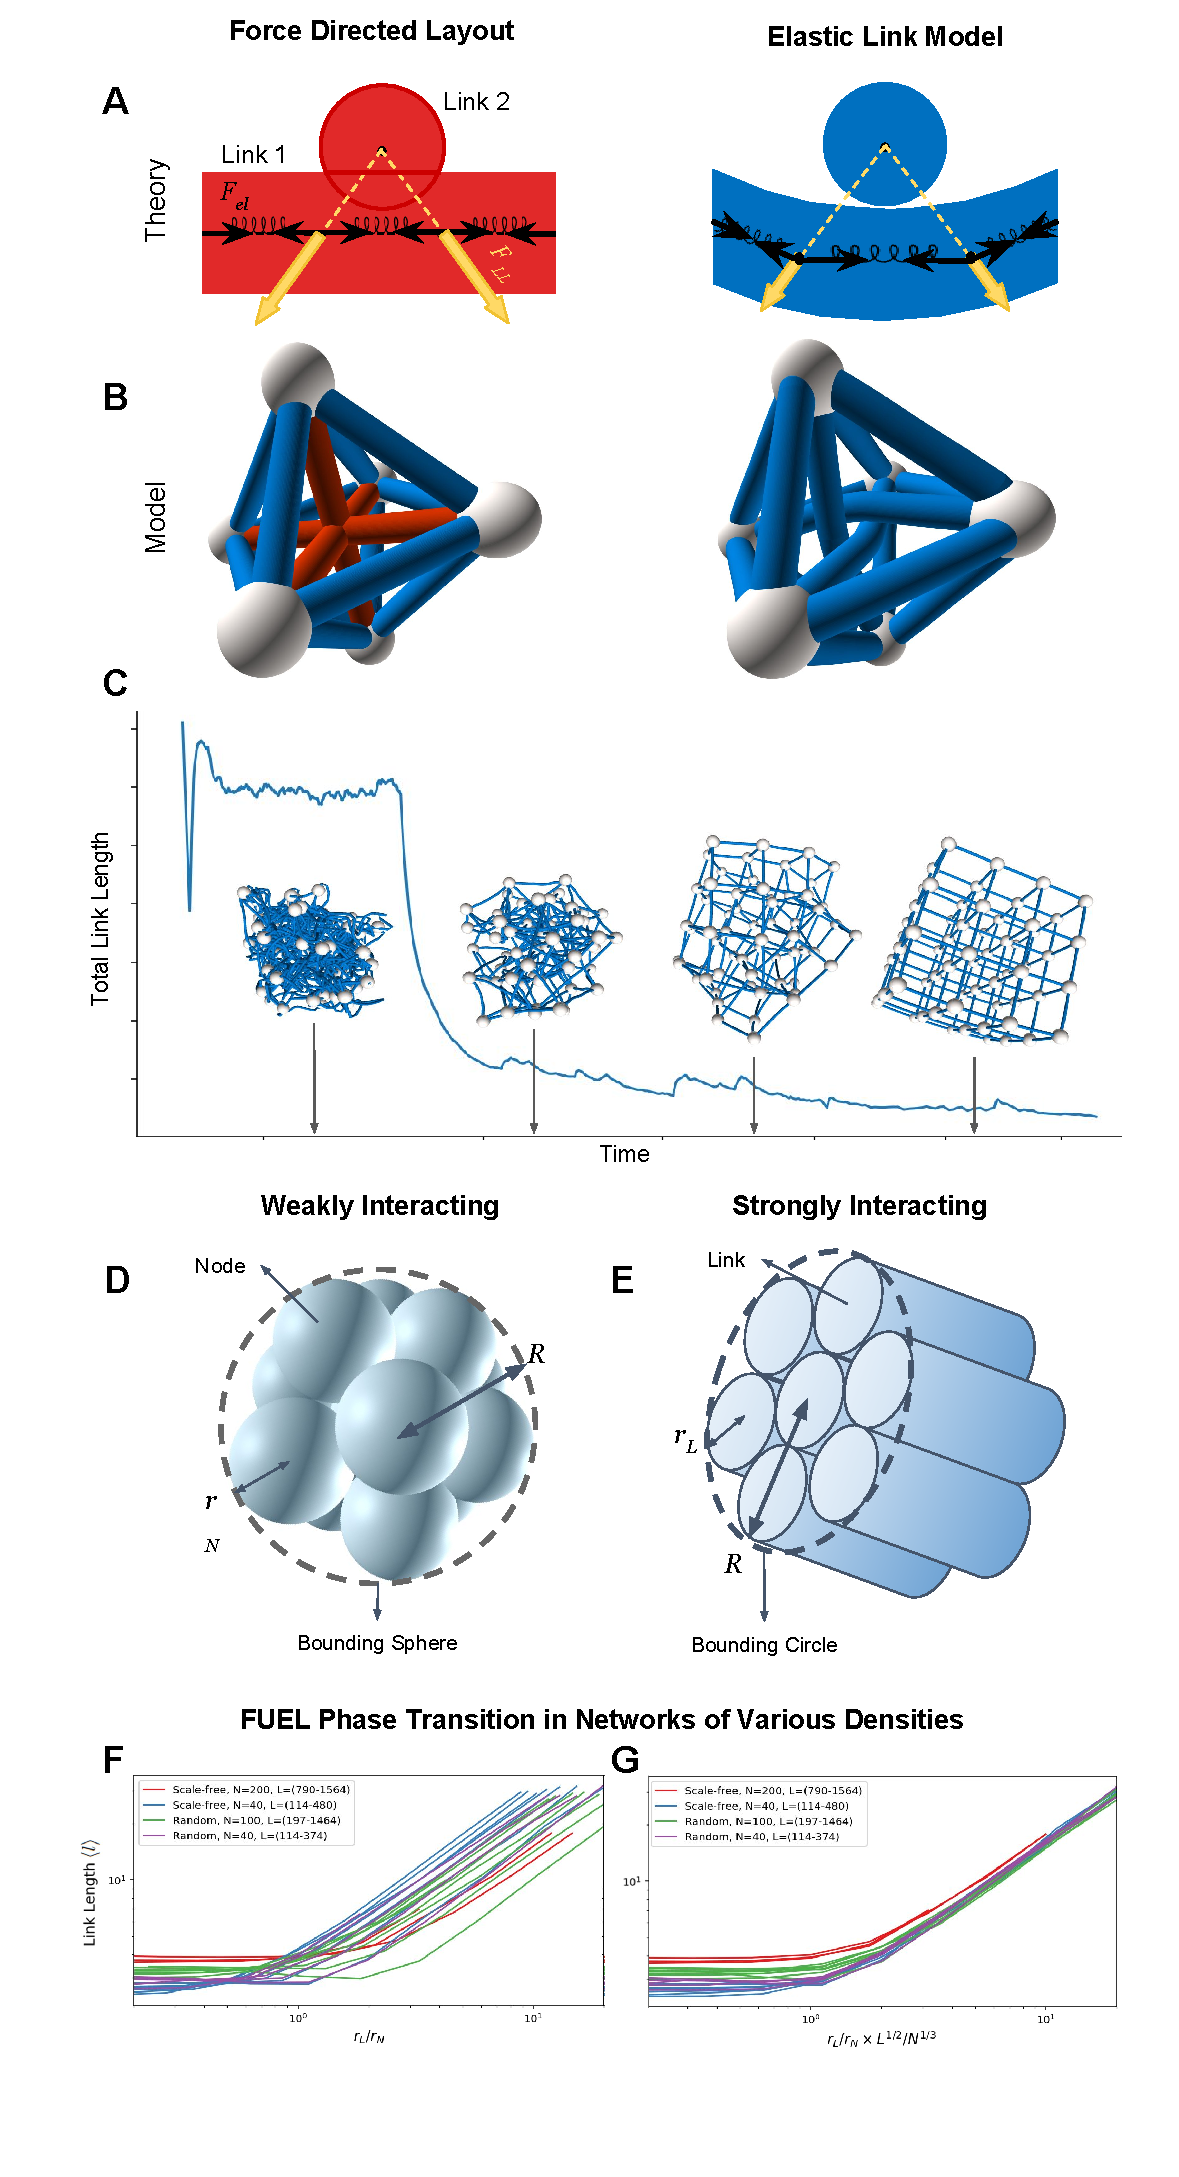
\includegraphics[width=.7\columnwidth]{fig-09-19/3d-crs-lat-trans-1.pdf}
    %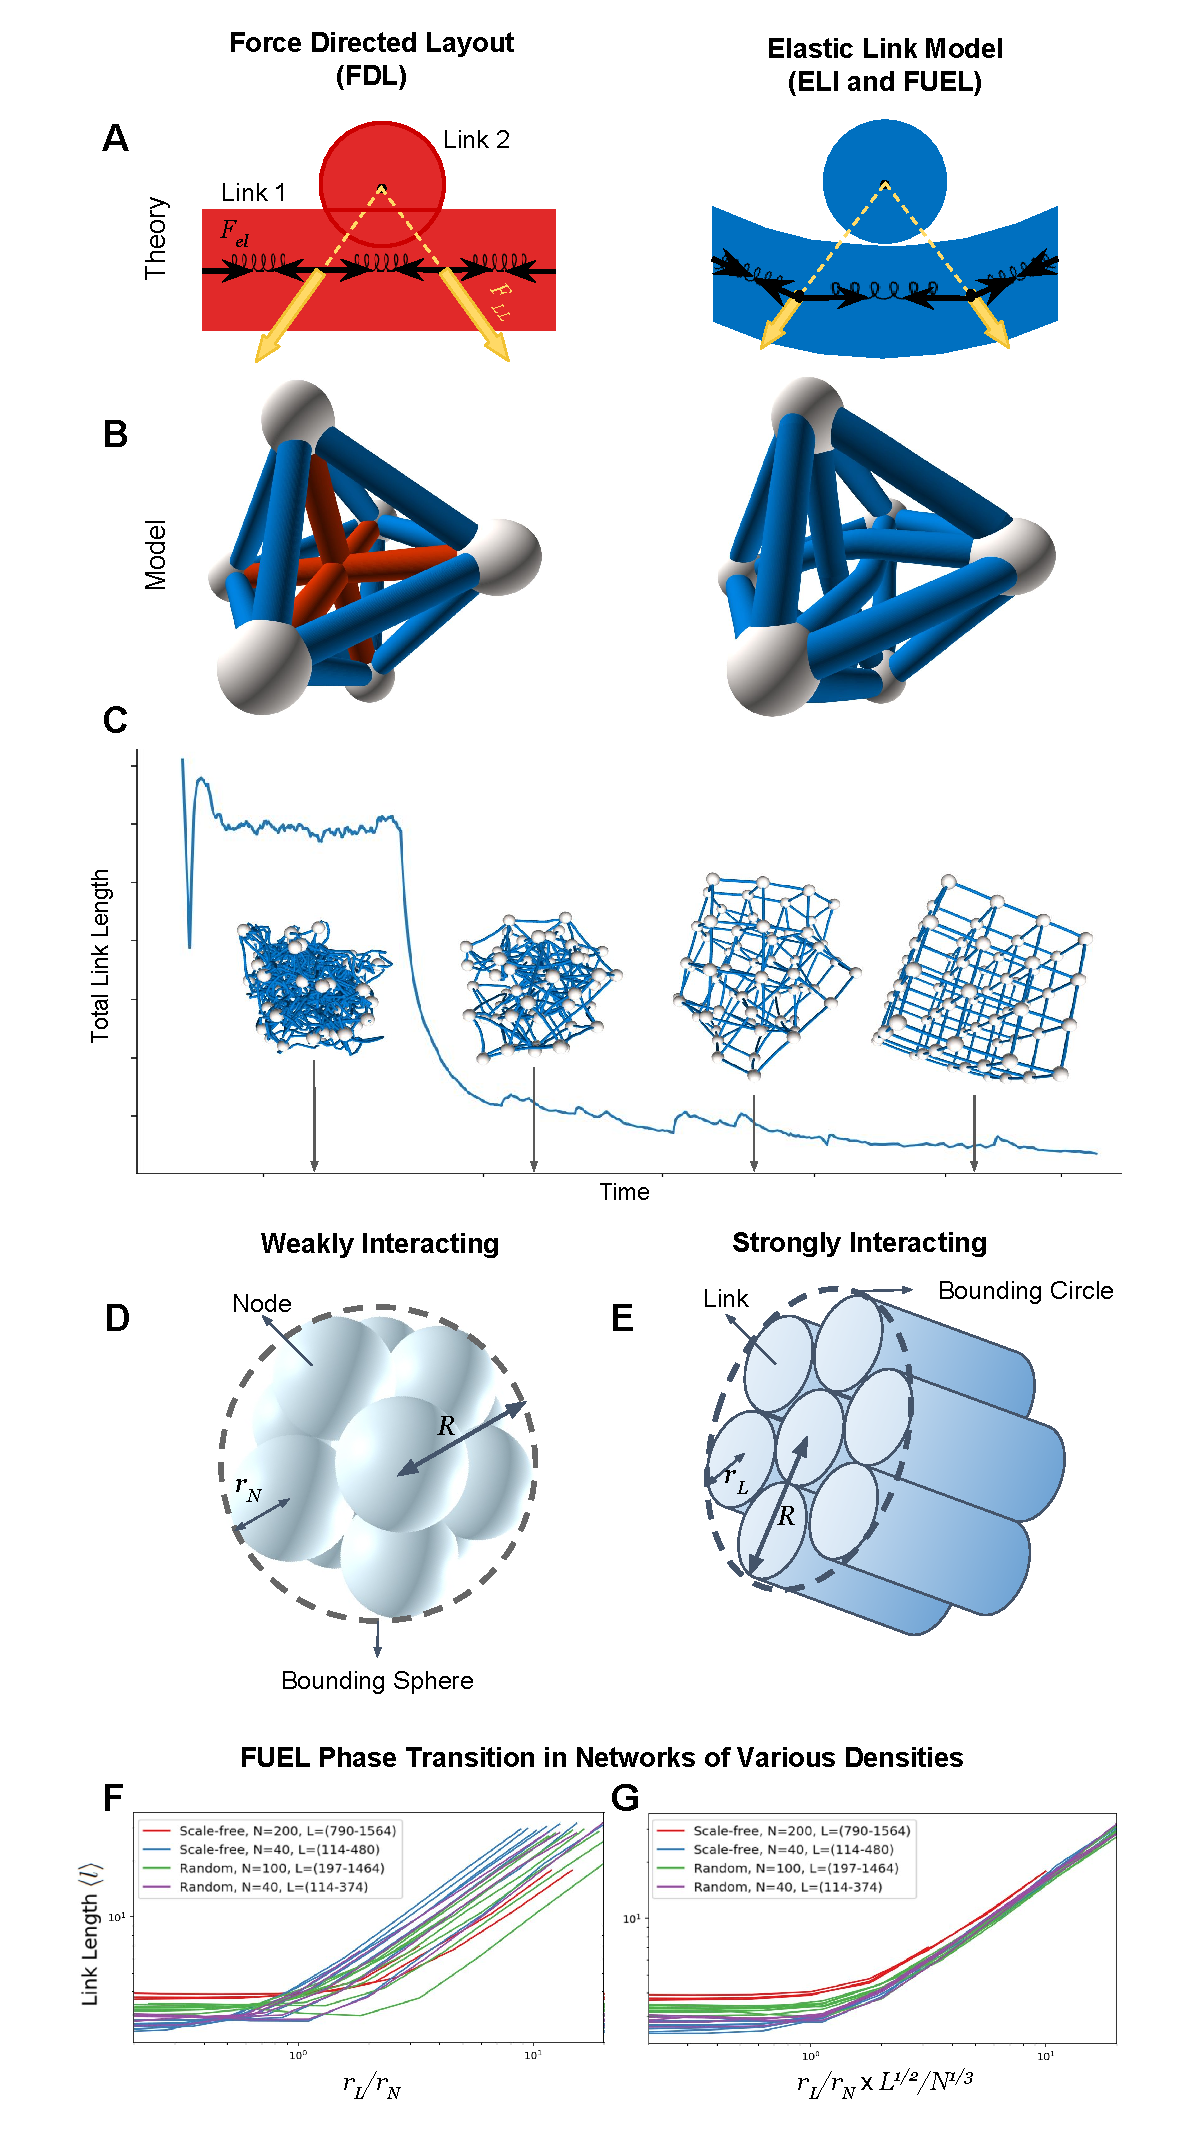
\includegraphics[width=.7\columnwidth]{fig-09-19/3d-crs-lat-trans-2.pdf}
    %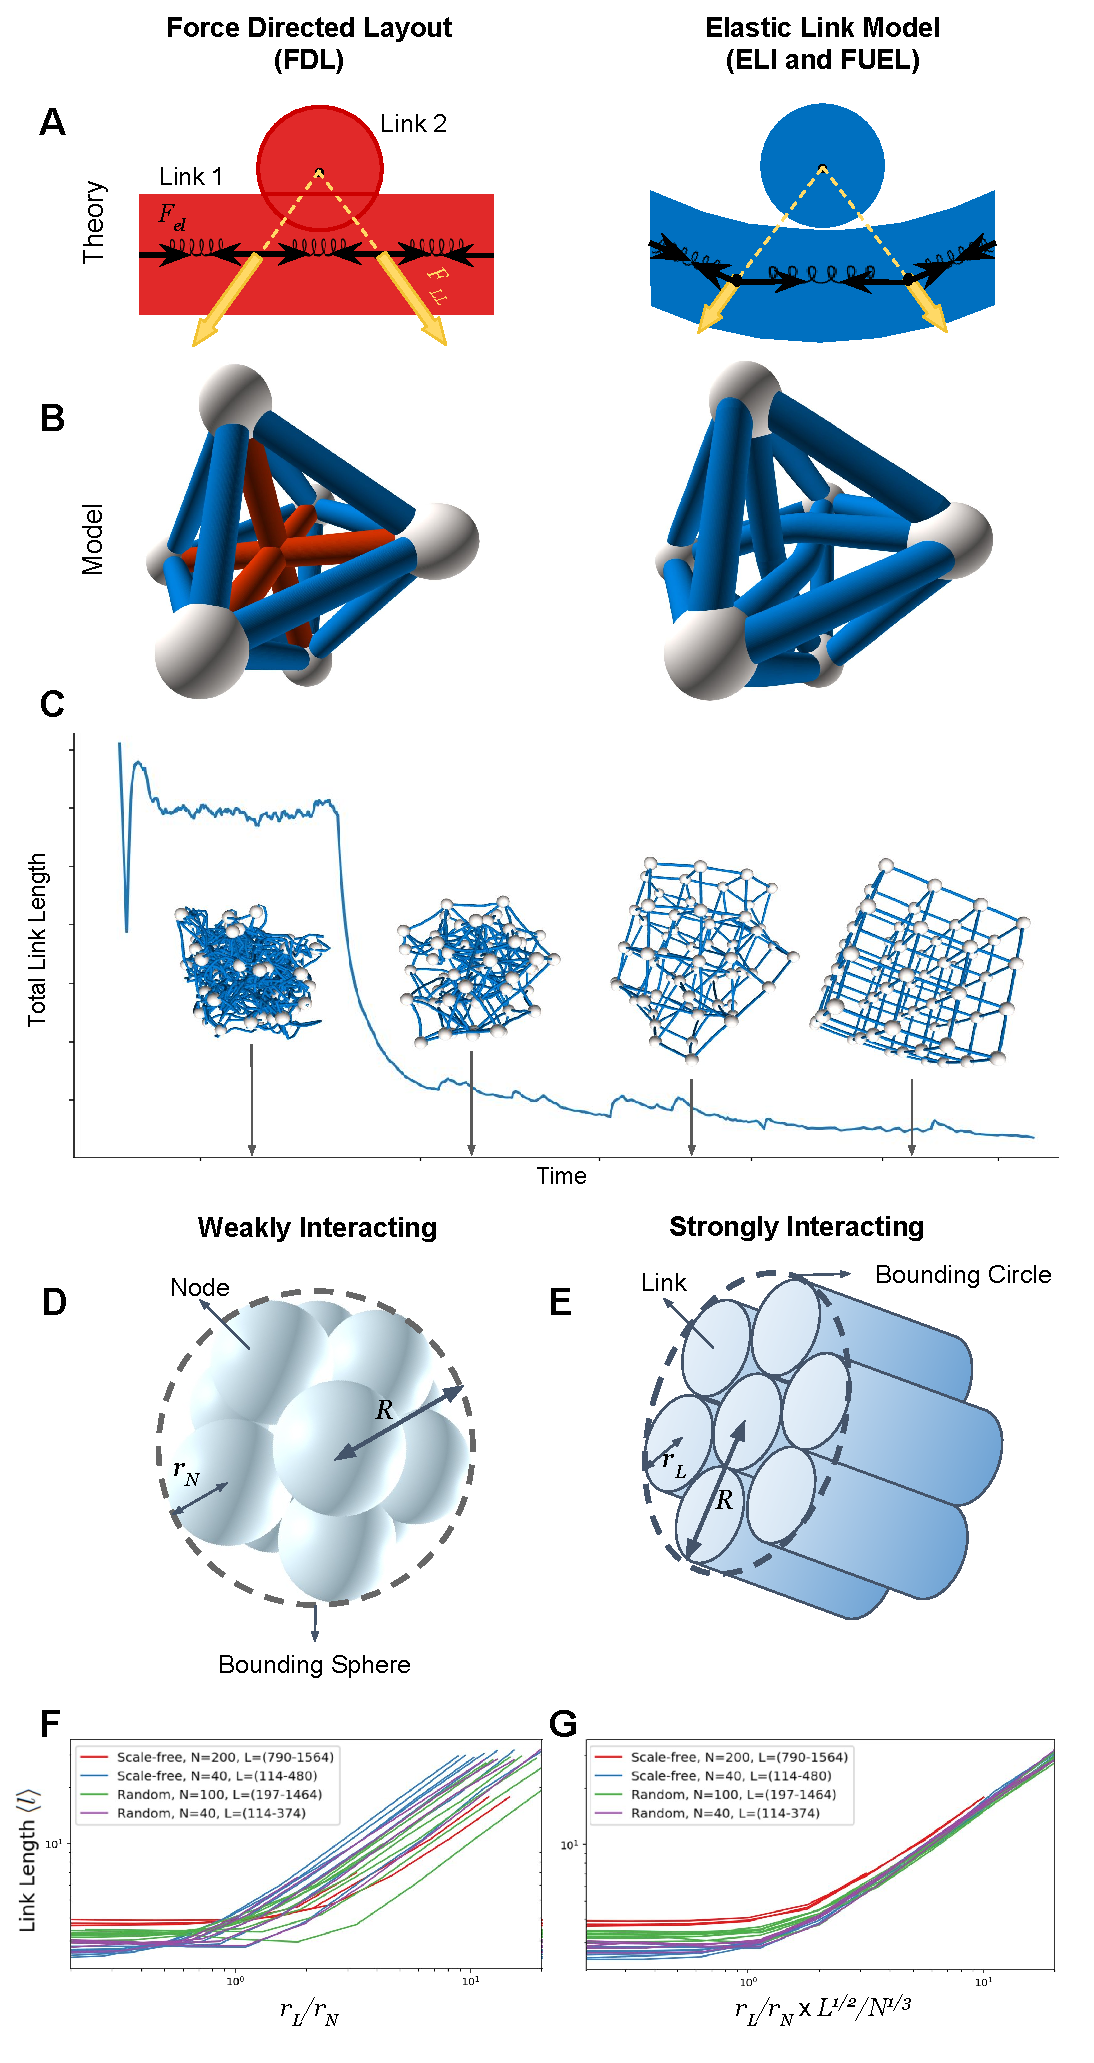
\includegraphics[width=.7\columnwidth]{fig-09-19/3d-crs-lat-trans-110317.pdf}
    %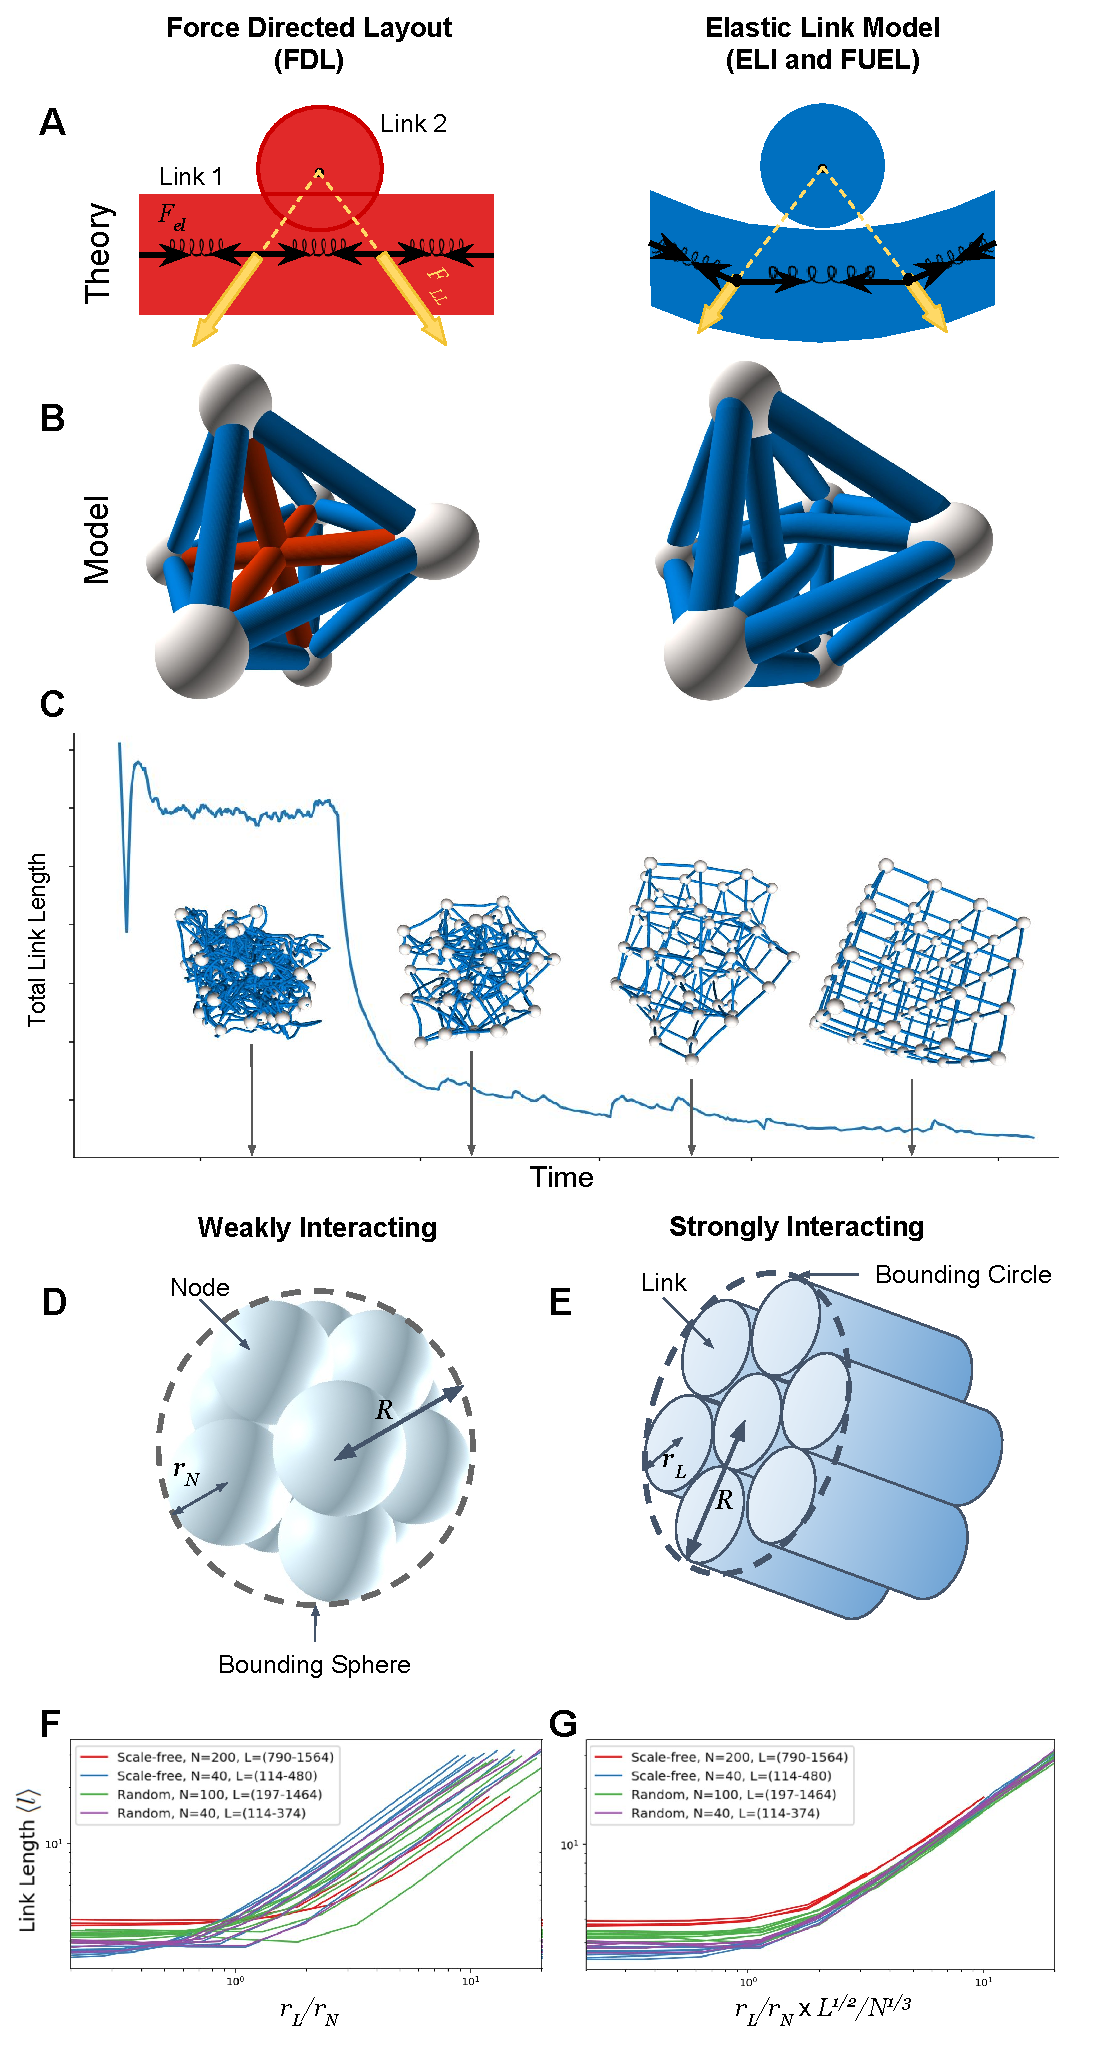
\includegraphics[width=.7\columnwidth]{fig-09-19/3d-crs-lat-trans-111917.pdf}
    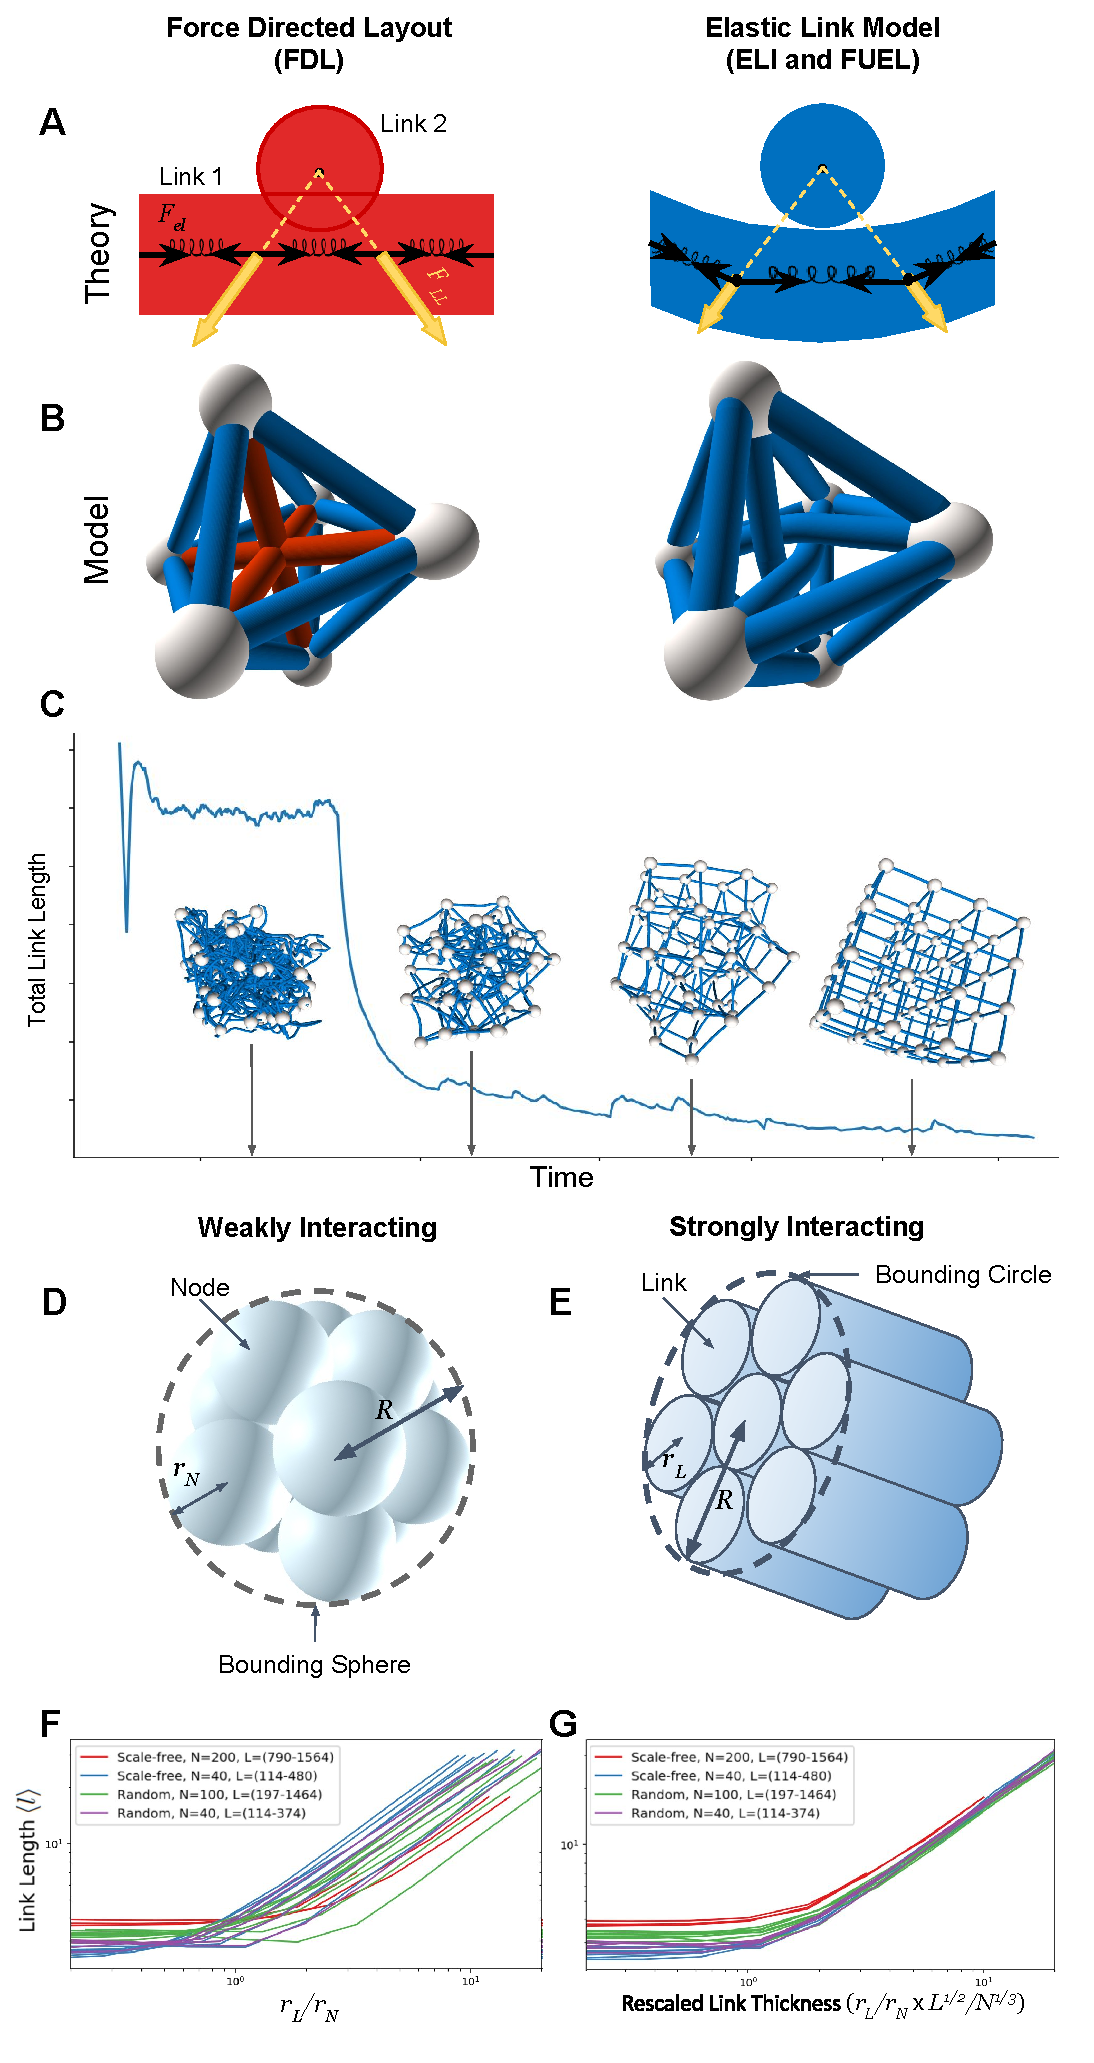
\includegraphics[width=.7\columnwidth]{fig-09-19/3d-crs-lat-trans-112017.pdf}
    \caption{
    \scriptsize
    {\bf(A) Modeling Framework:} We model each link as a stretched, flexible rubber band, 
    corresponding to many short springs connected to each other, pulled apart by
    elastic forces $F_{el}$. 
    The links exert a repulsive force $F_{LL}$  on each other that falls sharply at radii larger than $r_L$. 
    While in FDL the links cross each other (left figure), in ELI and FUEL such crossings are prohibited (right figure). 
    {\bf(B)} A small network with $N=6$ nodes laid out with FDL (left), resulting in multiple link crossings, shown as red links.   
    The right plot shows how the network laid out by ELI that resolves the crossings.
    {\bf (C)} Finding the final layout of a lattice with $r_L\ll r_N$, also showing the evolution of the total link length over time during the simulation. 
    We started from a random layout and used simulated annealing to find the final layout.
    The thermal noise helps links pass through each other and resolve crossings.
    {\bf (D)} In the weakly interacting region the links are thin ($r_L\ll r_N$), hence they interact only weakly with each other. 
    In this regime, the range of the node repulsion $r_N$ forces the nodes to stay within $2r_N$ of each other. 
    Therefore, the layout size can be estimated by finding the radius $R$ of the bounding sphere that surrounds $N$ balls, each of radius $r_N$. 
    {\bf (E)} Thick links exclude each other  in the strongly interacting regime. 
    %Almost all links will feel the push of other links along most of their length. 
    In the ideal scenario, with the least total volume, links are parallel with each other (\ref{ap:cross}). 
    In this case, the radius $R$ of the bounding circle determines the layout size, whose area is approximately the total cross-section of $L$ links. 
    {\bf (F)} The average link length versus $r_L/r_N$ for three with different $N$ and $L$ and geometries (random, scale-free). 
    The geometrical phase transitions are at different $r_L/r_N$ values. 
    {\bf (G)} Rescaling the ratio of $r_L/r_N$ using \eqref{eq:trans}  collapses the transition point, % on similar curves with phase transition happening around near $1$, 
    confirming the validity of \eqref{eq:trans}. }
    \label{fig:trans}
    \label{fig:crs-lat}
\end{figure}

To lay out physical networks, we must arrange the links and the nodes in such a way to avoid crossing each other, while minimizing the total link length. 
In other words, we must find the shortest path for each link, even when the straight path is obstructed by other nodes and links, a problem equivalent to stretching a rubber band between flexible obstacles (see Fig. \ref{fig:crs-lat}, also \ref{ap:affine} for proof \cite{novikov1984}). 
To achieve this we propose a model in which the forces governing the motion of the nodes and links is determined by the gradient of the total potential energy,  
\begin{align}
    V &= V_{el} + V_{NL} +V_{NN} + V_{LL} \cr 
    &= {k\over 2}\sum_l\int ds_l \left|{d\vec{x}_l\over ds_l} \right|^2 + 
    \left. k\sum_{i=1}^N  \sum_{l\in <i>}  \vec{X}_i \cdot{d\vec{x}_l%\pr{l^{(\mathrm{end})}_l} 
    \over ds_l}\right|_{s_l = s_l^{(\mathrm{end})}}
    \cr
    &+ A_N\sum_{i\ne j}  \exp\left[- {|\vec{X}_i-\vec{X}_j|^2 \over 4r_N^2}\right]+A_L\sum_{l\ne m} \iint ds_lds_m 
    \exp\left[- {|\vec{x}_l-\vec{x}_m|^2 \over 4 r_L^2}\right] ,
 \label{eq:Vfull}
\end{align}
where $V_{el}$ is the total elastic potential of all links $l=1,...,L$. 
Each link is modeled as an elastic cylinder with radius $r_L$, experiencing both internal elastic forces and short-range external repulsive forces from other links and nodes. $V_{NL}$ captures the node-link interactions at link endpoints;
the non-crossing condition is ensured by a short-range repulsive force in
$V_{NN}$  (node-node interaction)  and  $V_{LL}$ (link-link interaction) modeled as short-range Gaussian potentials whose strength is set by $A_N$ and $A_L$. 
In \eqref{eq:Vfull} $s_l$ is the length parameter of link $l$ and  $\vec{x}_l(s_l,t)$ represents the position of a point along the center of the link at time $t$;
%$s_l^\mathrm{(end)}$ is the parameter value at the endpoints of link $l$;
%$l\in <i>$ represents the set of links connected to node $i$; 
$\vec{X}_i(t)$ is the position of node $i$; $r_N$ is the range of the node-node repulsive force; $k$ is the elastic constant of the links.
The lowest energy solution of \eqref{eq:Vfull} can lead to sharp bending of some links, which we avoid using a Gay-Berne potential \cite{gay1981modification} %\cite{gay1981modification,berne1972gaussian}
employed in polymer physics %\citep{everaers2003interaction,babadi2006coarse,mergell2003modeling,cleaver1996extension}
\citep{everaers2003interaction,babadi2006coarse} (\ref{ap:ell}). 
Finally, we embed the network in a high viscosity medium, allowing it to relax to a low energy state without oscillations.
Therefore, the node and link positions follow the first order gradient descent equations of motion, 
\begin{align}
    \lambda_N {dX_i\over dt} &= -{\ro V \over \ro X_i} %- \vec{\del}_{\vec{X}_i} \left[V_{\mathrm{NL}} + V_{NN} \right]
    \label{eq:nodes},\\
    \lambda_L {dx_l \over dt} & =  -{\ro V \over \ro x_l} + {d\over ds_l} {\ro V \over \ro (dx_l /ds_l)}   \label{eq:Langevin0},
\end{align}
where $\lambda_N$ and $\lambda_L$ are the node and link friction constants (\ref{ap:eom}). 
We use FDL to set the initial node positions and explore two versions of the model with different constraints: 
(i) In the Elastic Link Model (ELI), which corresponds to $\lambda_N\to \infty$, the node positions are kept fixed and only the links are allowed to reorganize themselves; 
(ii) In the Fully Elastic Model (FUEL) we assume $\lambda_N \sim \lambda_L$, hence both nodes and links are free to move. 
%To obtain the optimal layout, we run  \eqref{eq:nodes}--\eqref{eq:Langevin0} until the forces on the right vanish, obtaining the equilibrium state corresponding to a minimum of \eqref{eq:Vfull}.

Equations \eqref{eq:Vfull}--\eqref{eq:Langevin0} represent a special case of manifold dynamics, frequently used in polymer physics \cite{mezard1991replica}. 
The network has an uneven potential energy landscape \cite{bouchaud1998out} %\cite{parisi2002physical} 
with a very large number of local minima, hence identifying the globally optimal configuration is NP hard (\ref{ap:np}).
We therefore use simulated annealing \cite{kirkpatrick1987optimization} %\cite{hwang1988simulated} 
to approach an energetically favorable local minimum (\ref{ap:np}). 
Figure \ref{fig:crs-lat}C shows how FUEL finds the correct 3D configuration of a lattice, %(\ref{ap:np}), 
helped by the noise to tunnel through the finite potential walls and escape local minima. 

%To understand the challenges ELI and FUEL must resolve, we start with 
%If we do consider 
%FDL, which assigns spring-like attractive forces between linked node pairs, and repulsive forces between all node pairs to avoid collapse. 
As FDL ignores the physical dimensions of the nodes and links% (Fig. \ref{fig:crs-lat})
, it suffers from multiple link and node crossings (\ref{ap:cross}). % for nonzero $r_L$ (Fig. \ref{fig:phase-compare}A), which it cannot resolve. %\ref{fig:crs-lat}A). 
The number of such conflicts increases linearly with $r_L$ (Fig. \ref{fig:phase-compare}A), a behavior analytically predicted by a geometric model (\ref{ap:cross}). %\cite{kabourov2015spring}. 
To avoid these conflicts, we applied ELI and FUEL to several networks with different topologies (regular lattice, random, scale-free), spanning a range of sizes and link densities. 
We find that the obtained layouts undergo a visually detectable geometrical transition as we increase the link thicknesses (Fig. \ref{fig:phase-compare}E, F, I, J). 
The transition is also confirmed by the relaxation time, representing the characteristic time the simulation needs to find an equilibrium solution. The strong peak in the relaxation time for FUEL near $r_L^c$ (Fig. \ref{fig:phase-compare}D)
%In FUEL, the relaxation time reaches a peak at the transition
%as would be expected from 
documents a critical slowing down commonly in systems undergoing a second order phase transition. 
Next we discuss the layout geometry, before and after this transition.% show layouts generated using ELI (A) and FUEL (B), also documenting a qualitative structural change as we increase $r_L$, as we discuss next.
\begin{figure}
\centering
%\vspace{-2cm}
%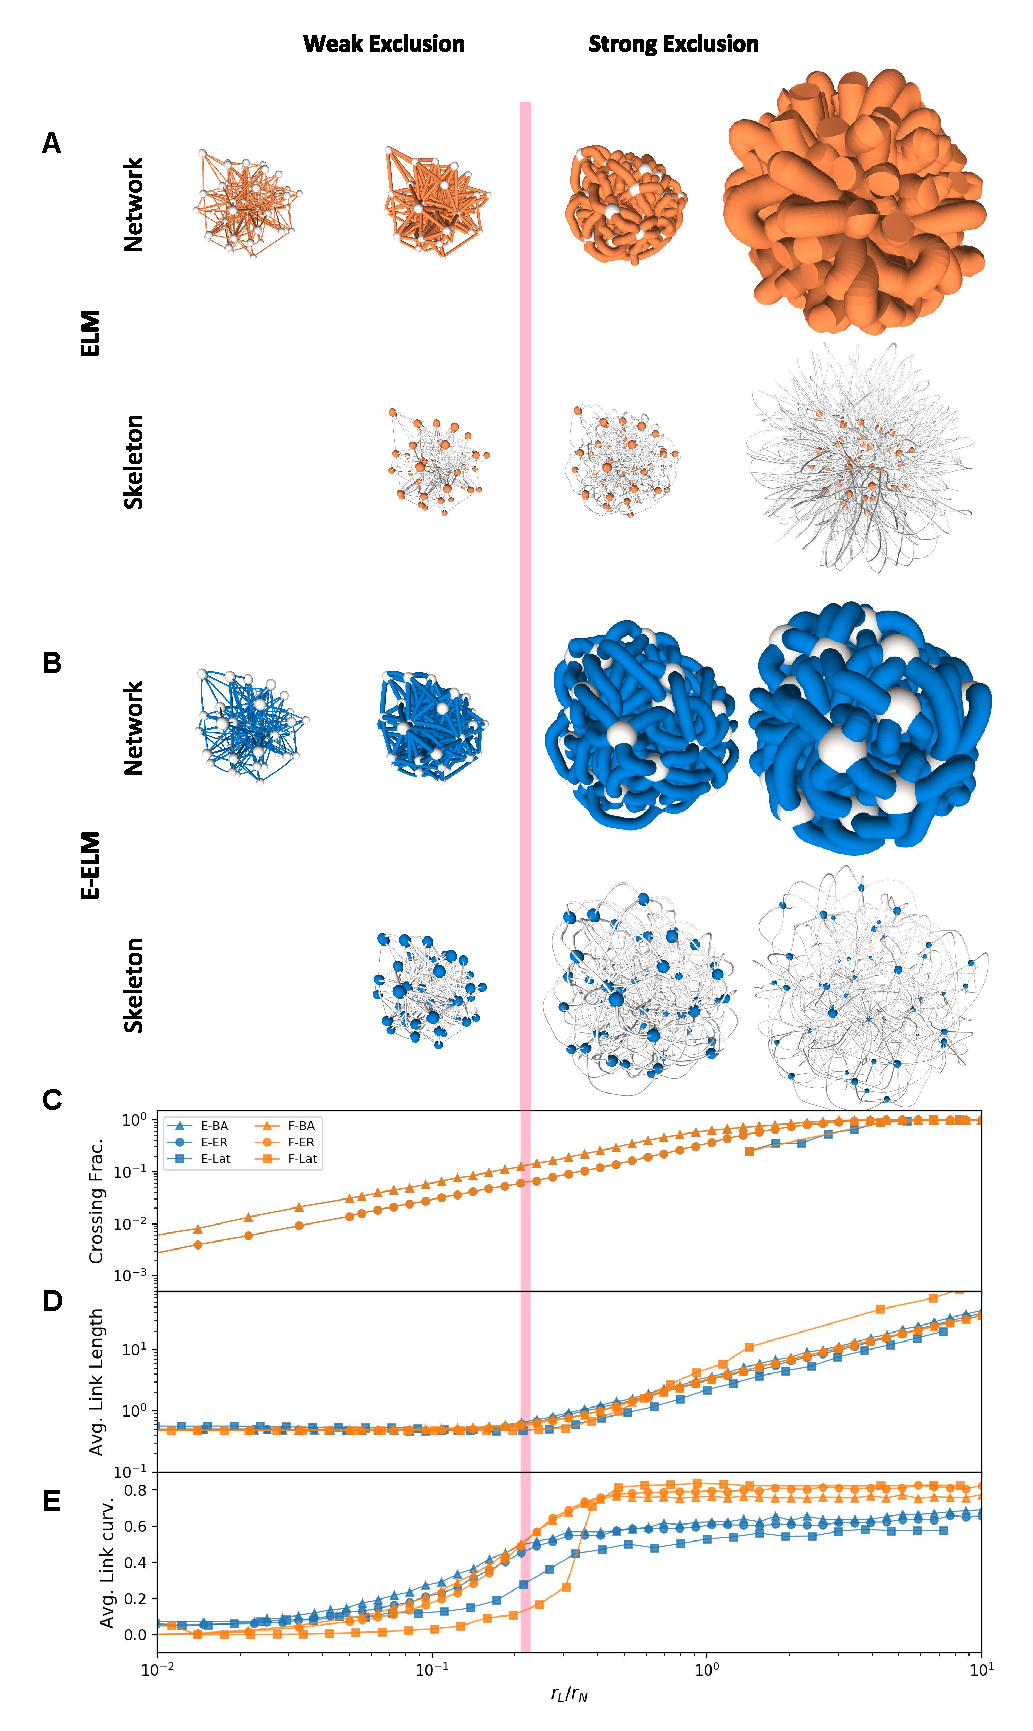
\includegraphics[width=.69\columnwidth]{fig-09-19/phase-051817.pdf}
% 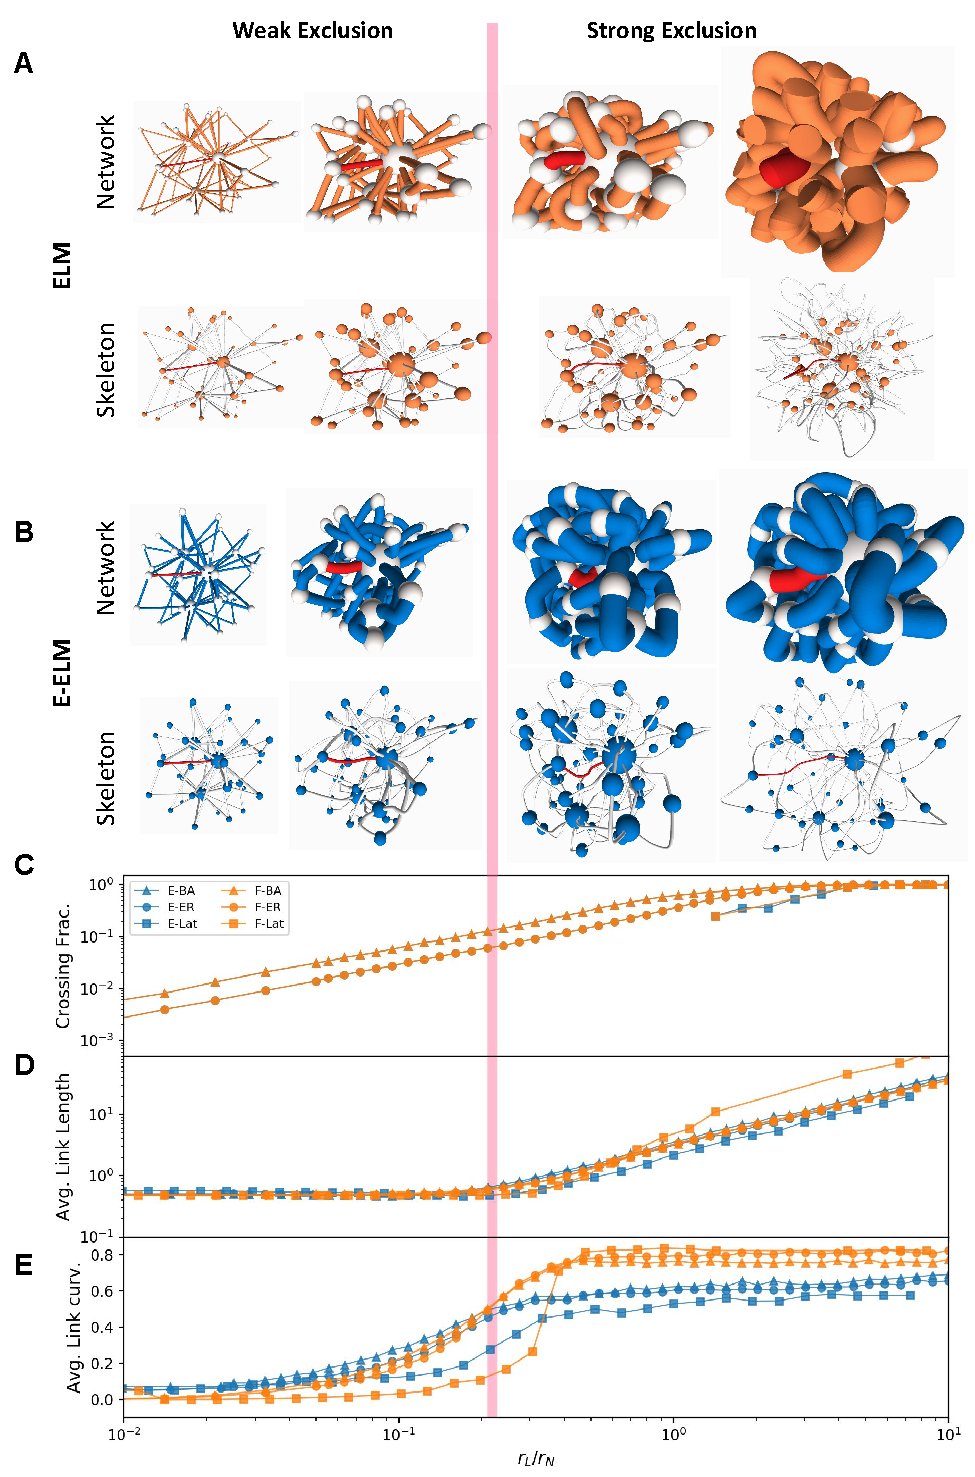
\includegraphics[width=.69\columnwidth]{fig-09-19/phase-061717.pdf}
% 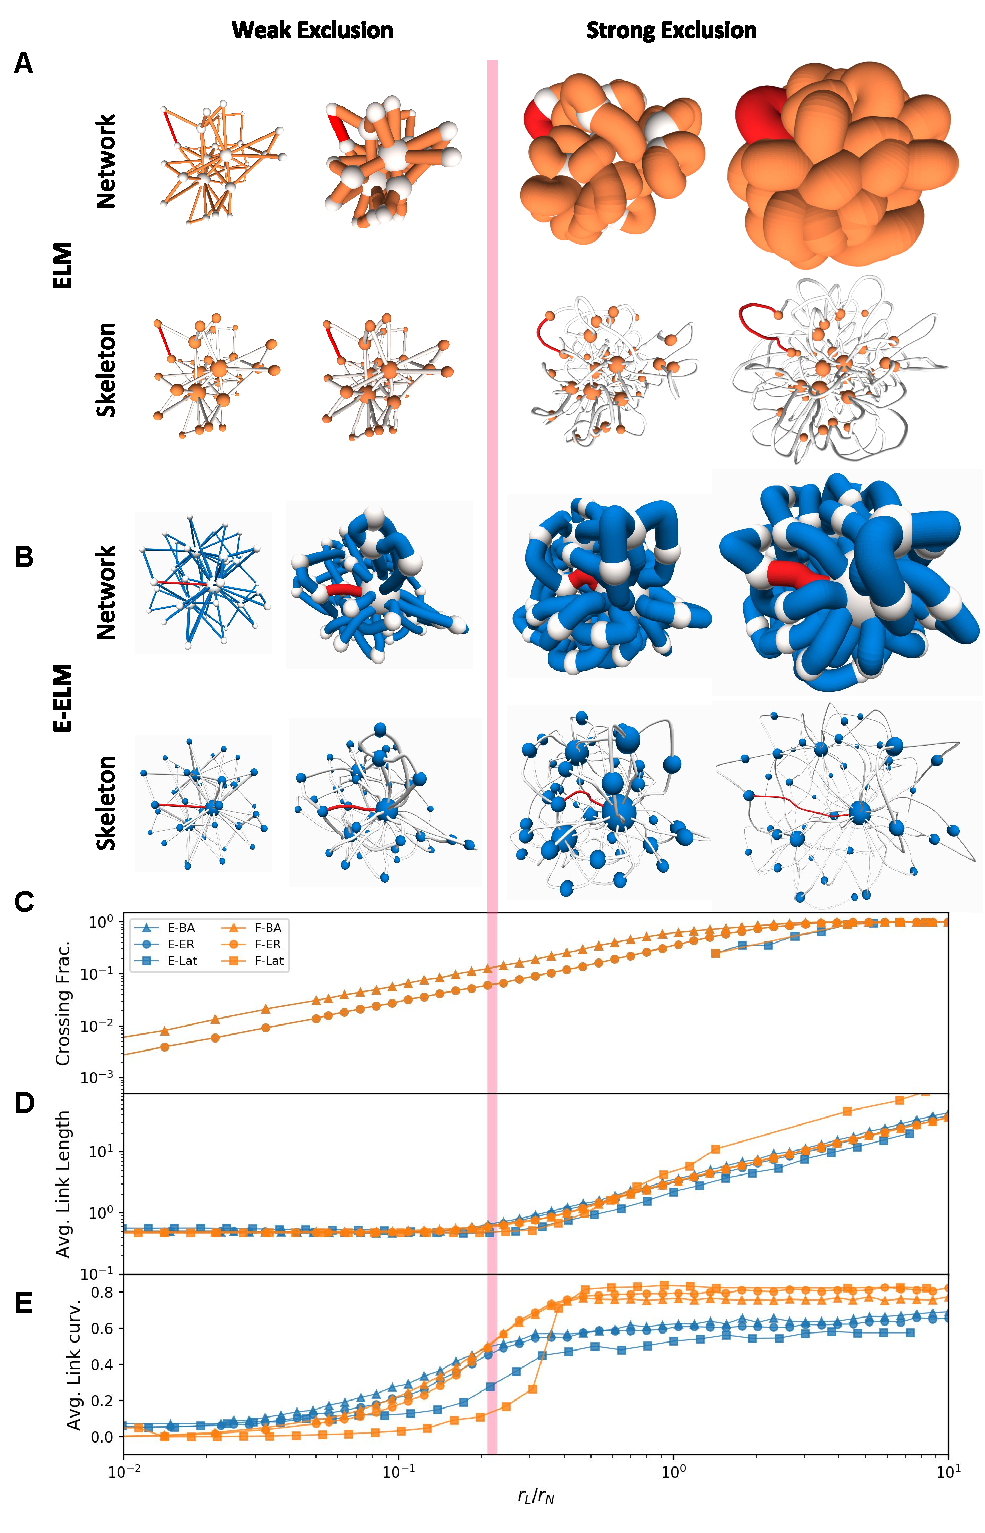
\includegraphics[width=.69\columnwidth]{fig-09-19/phase-071517.pdf}
% 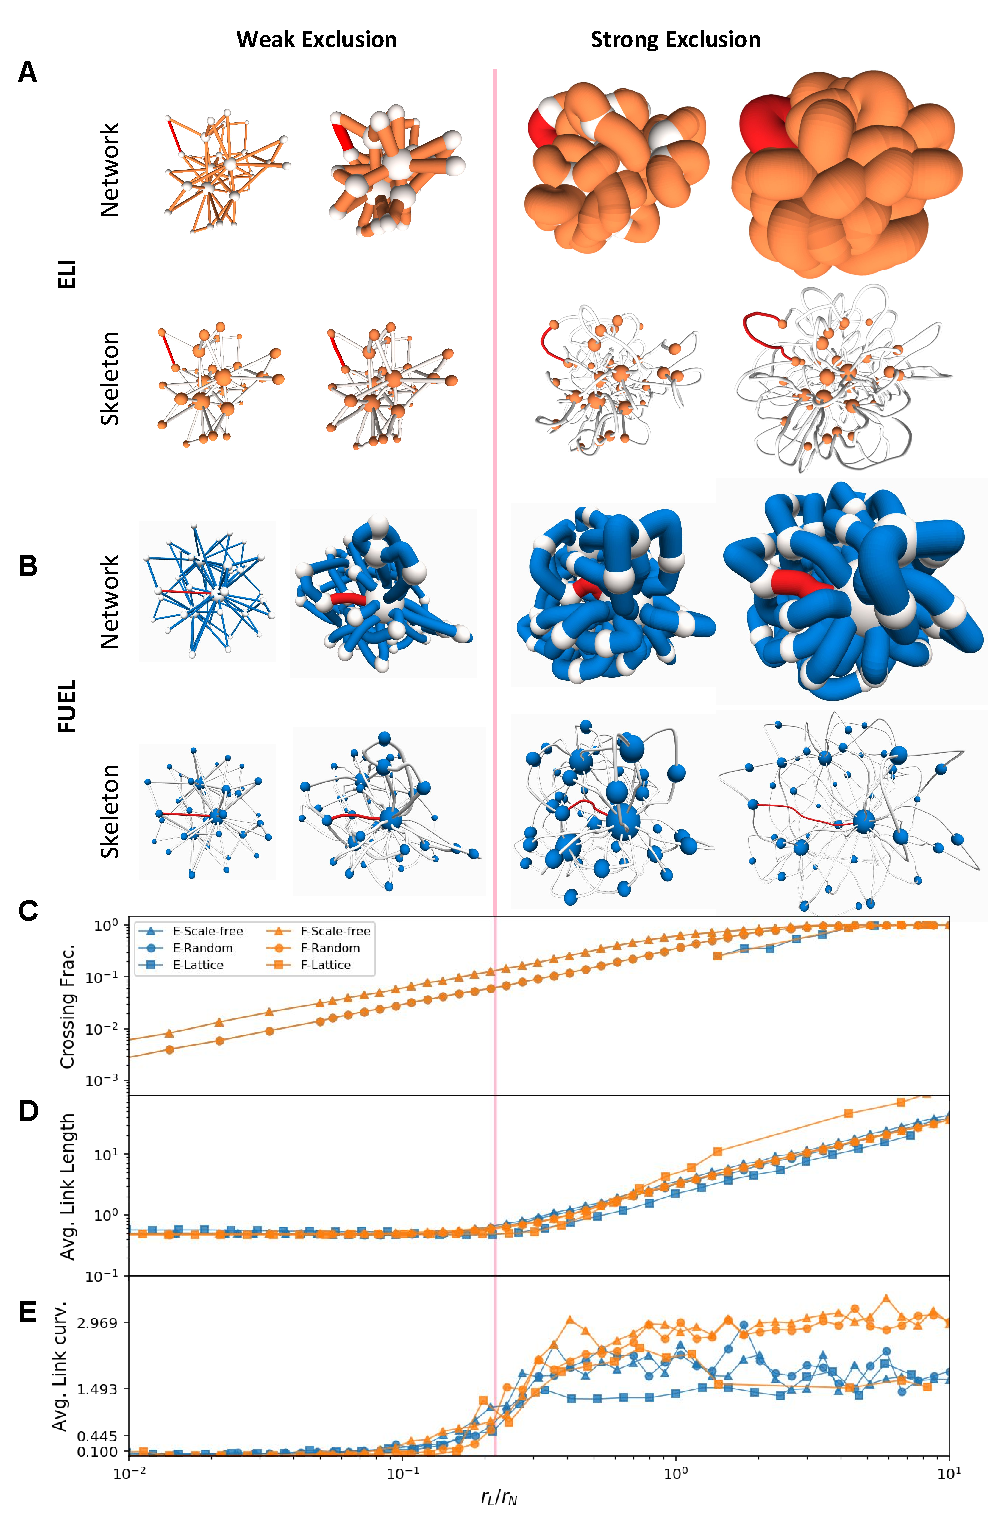
\includegraphics[width=.69\columnwidth]{fig-09-19/phase-full-071917.pdf}
%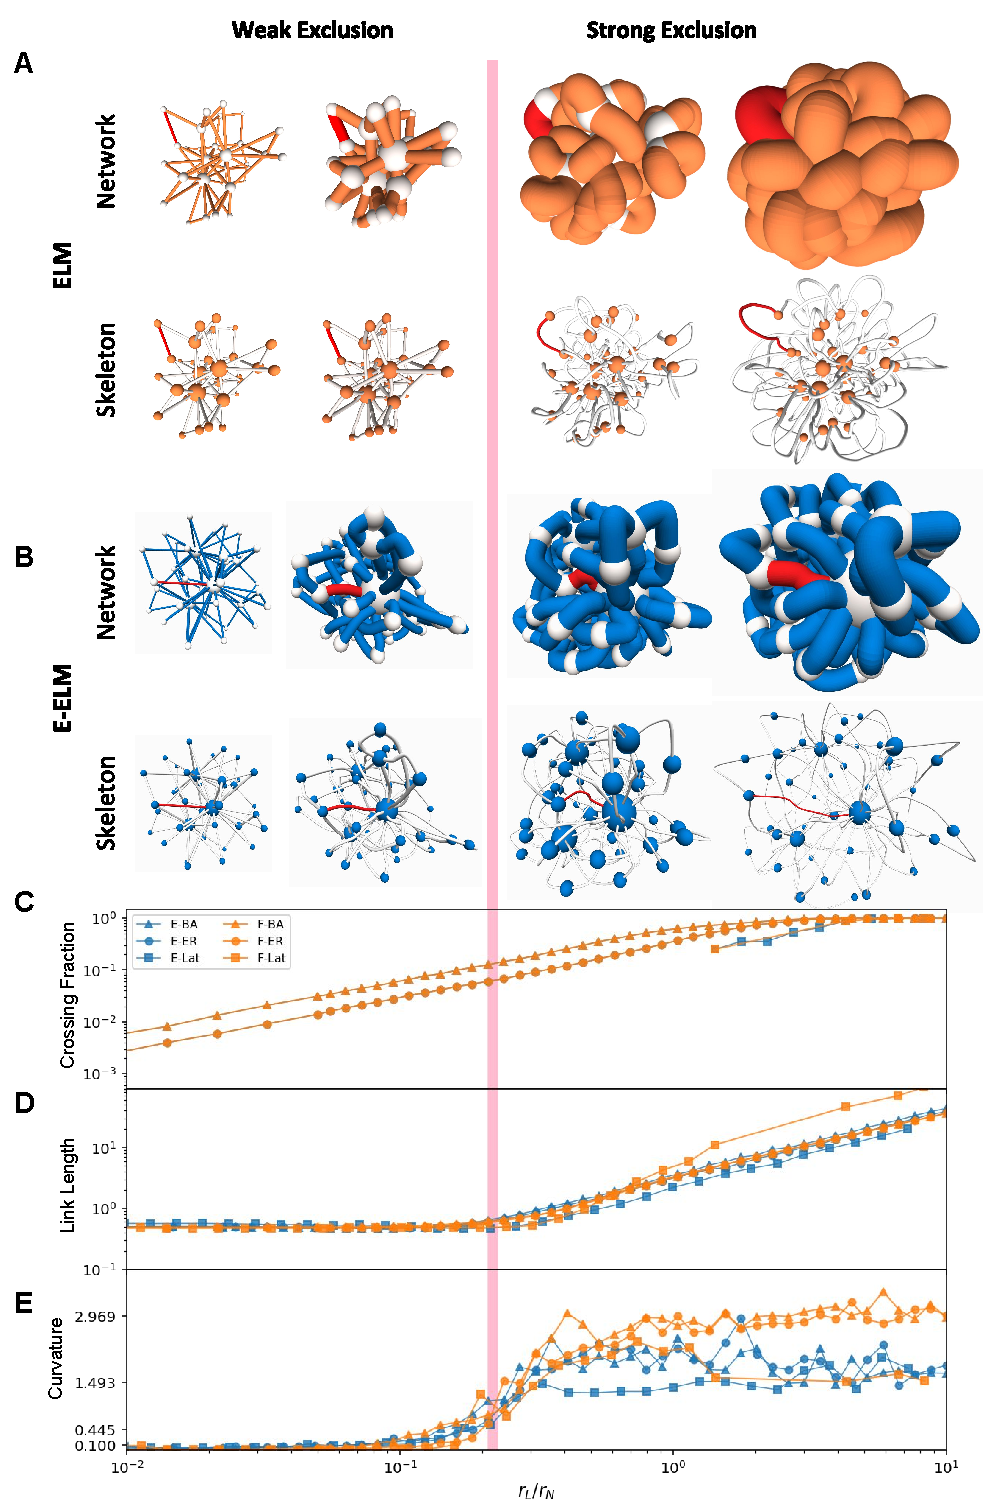
\includegraphics[width=.69\columnwidth]{fig-09-19/3D-phase.pdf}
%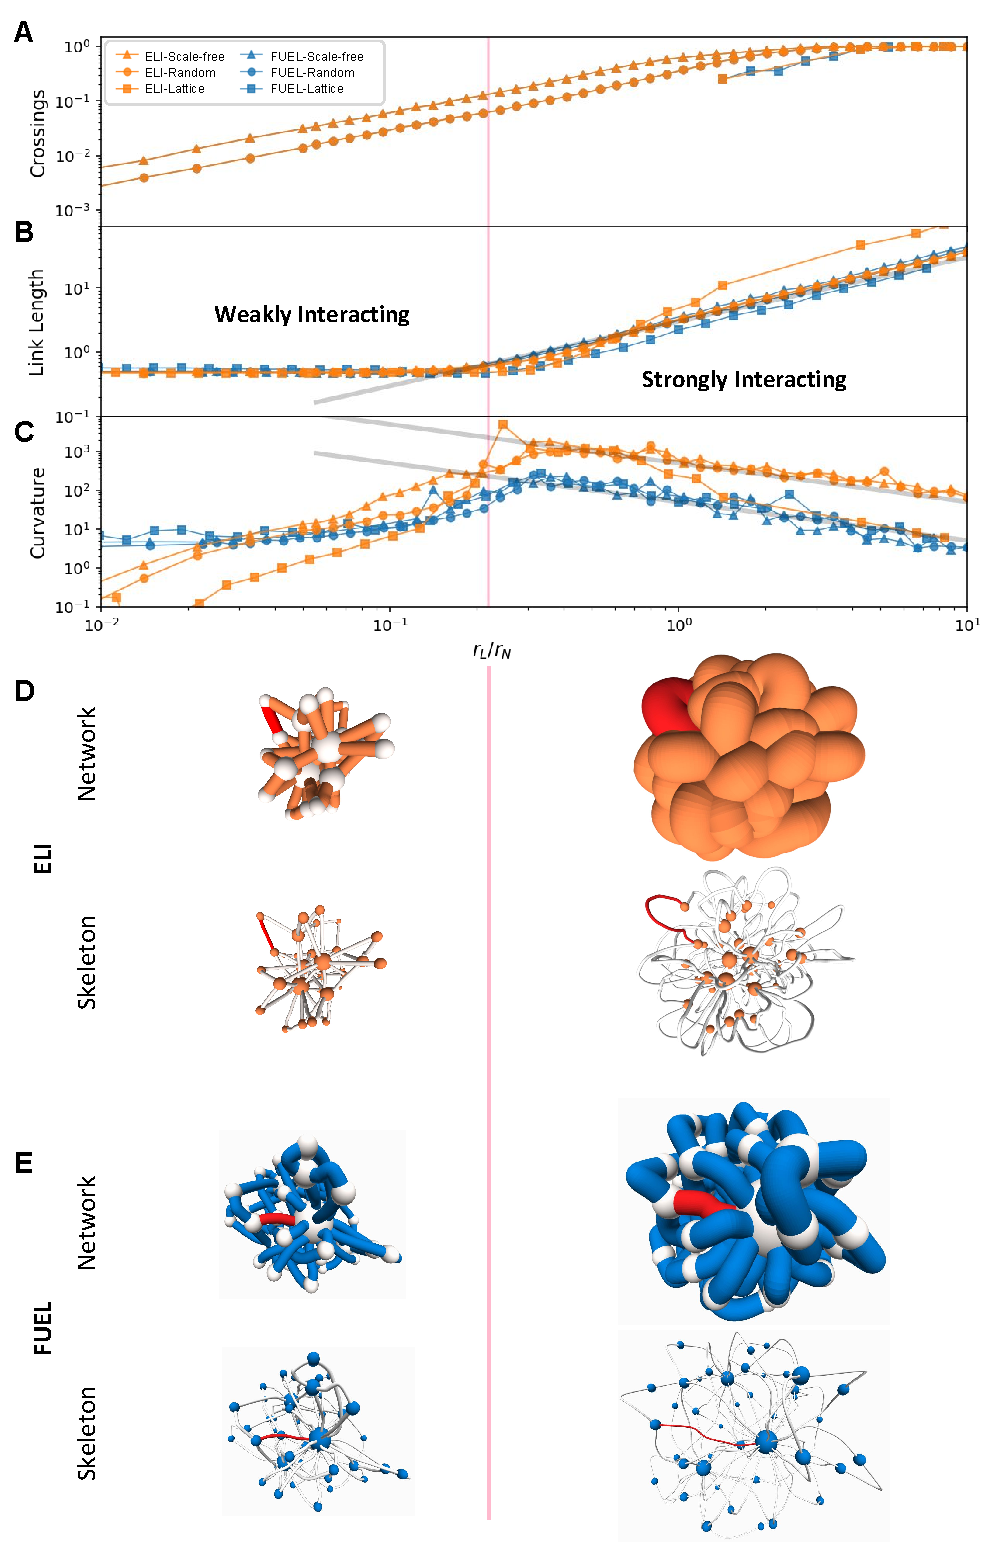
\includegraphics[width=.69\columnwidth]{fig-09-19/3D-phase-compare-092617.pdf}
%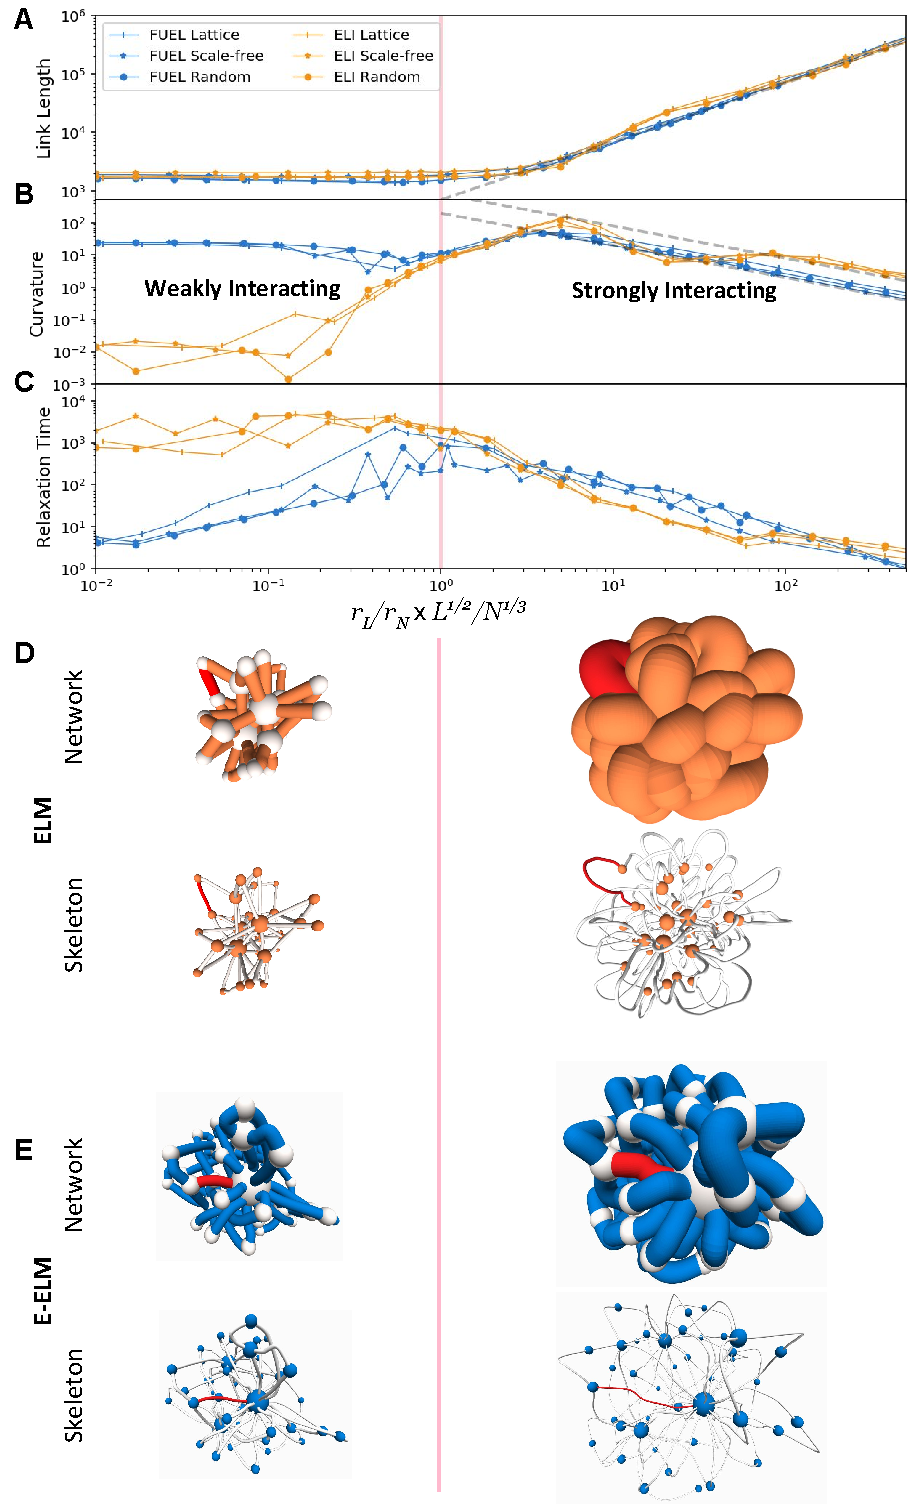
\includegraphics[width=.63\columnwidth]{fig-09-19/3D-phase-compare-102417.pdf}
% 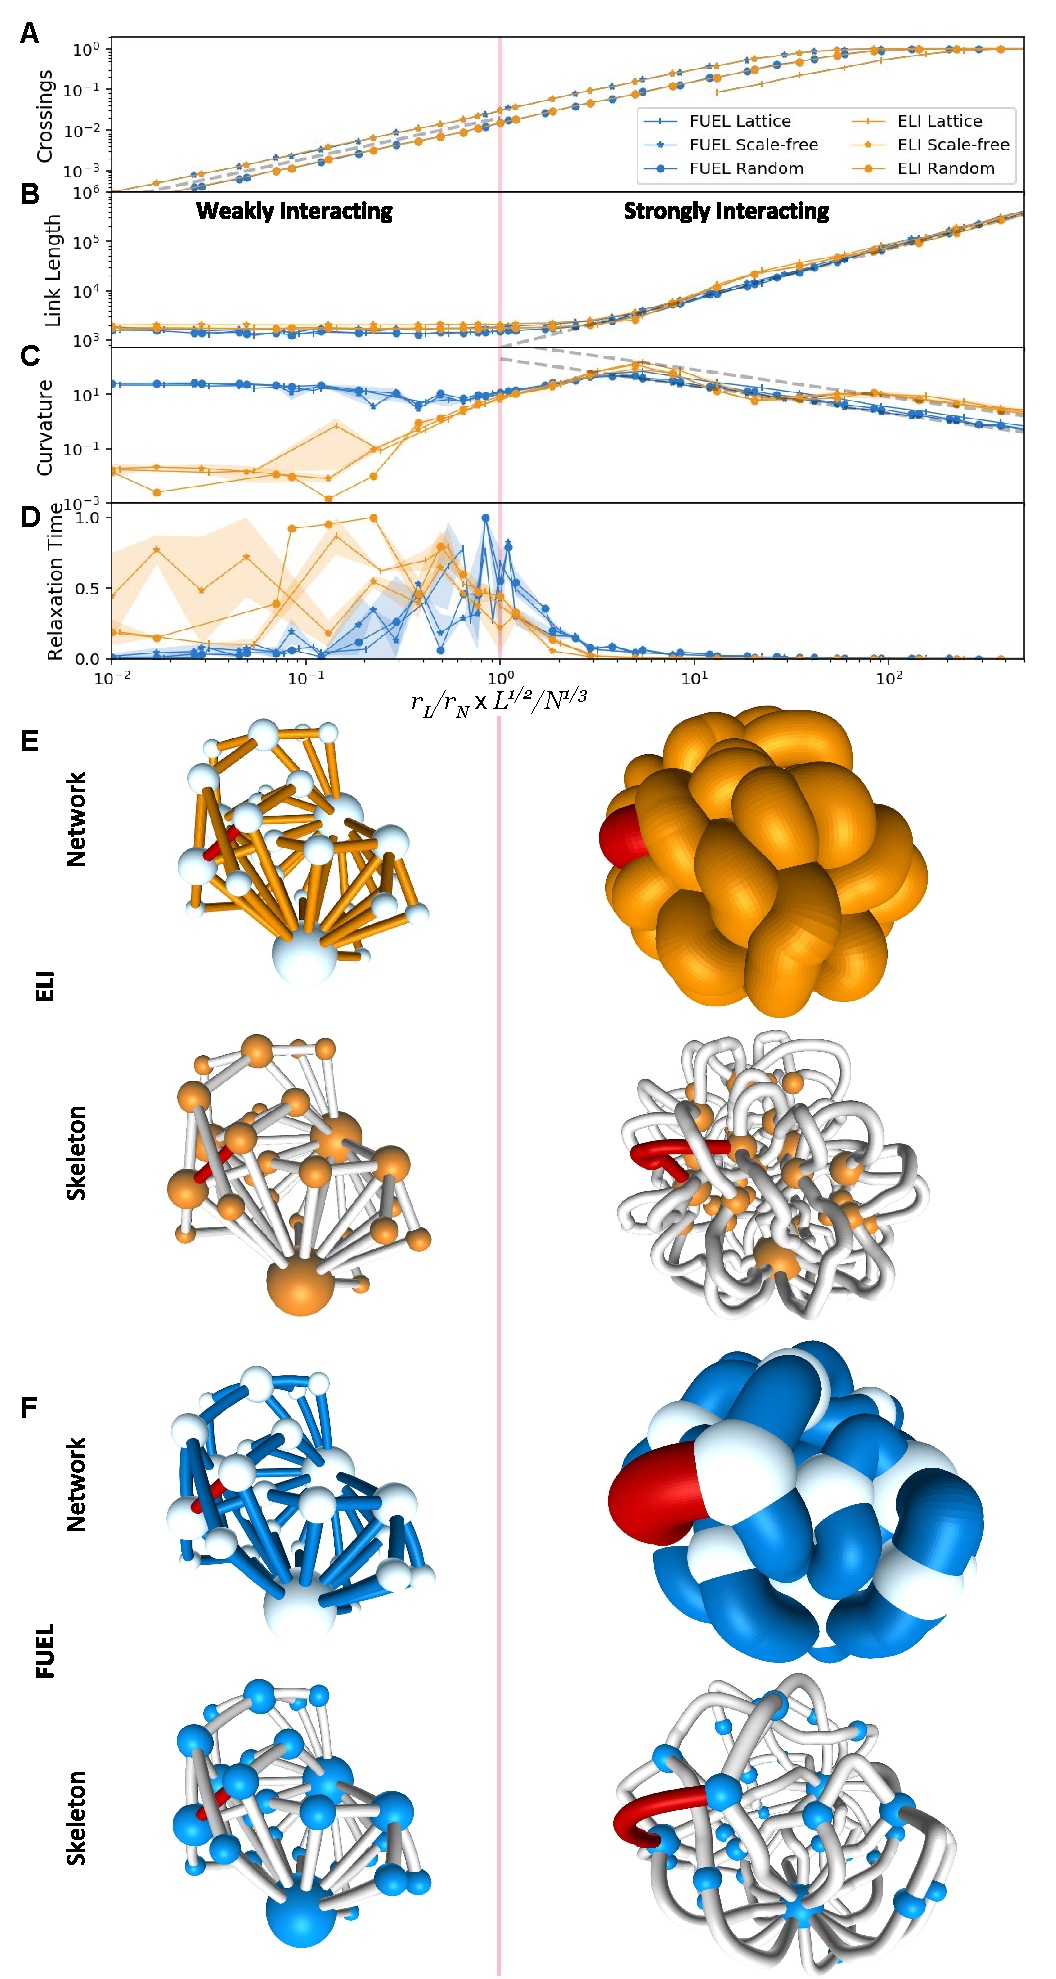
\includegraphics[width=.75\columnwidth]{fig-09-19/3d-phase-compare-102517.pdf}
% 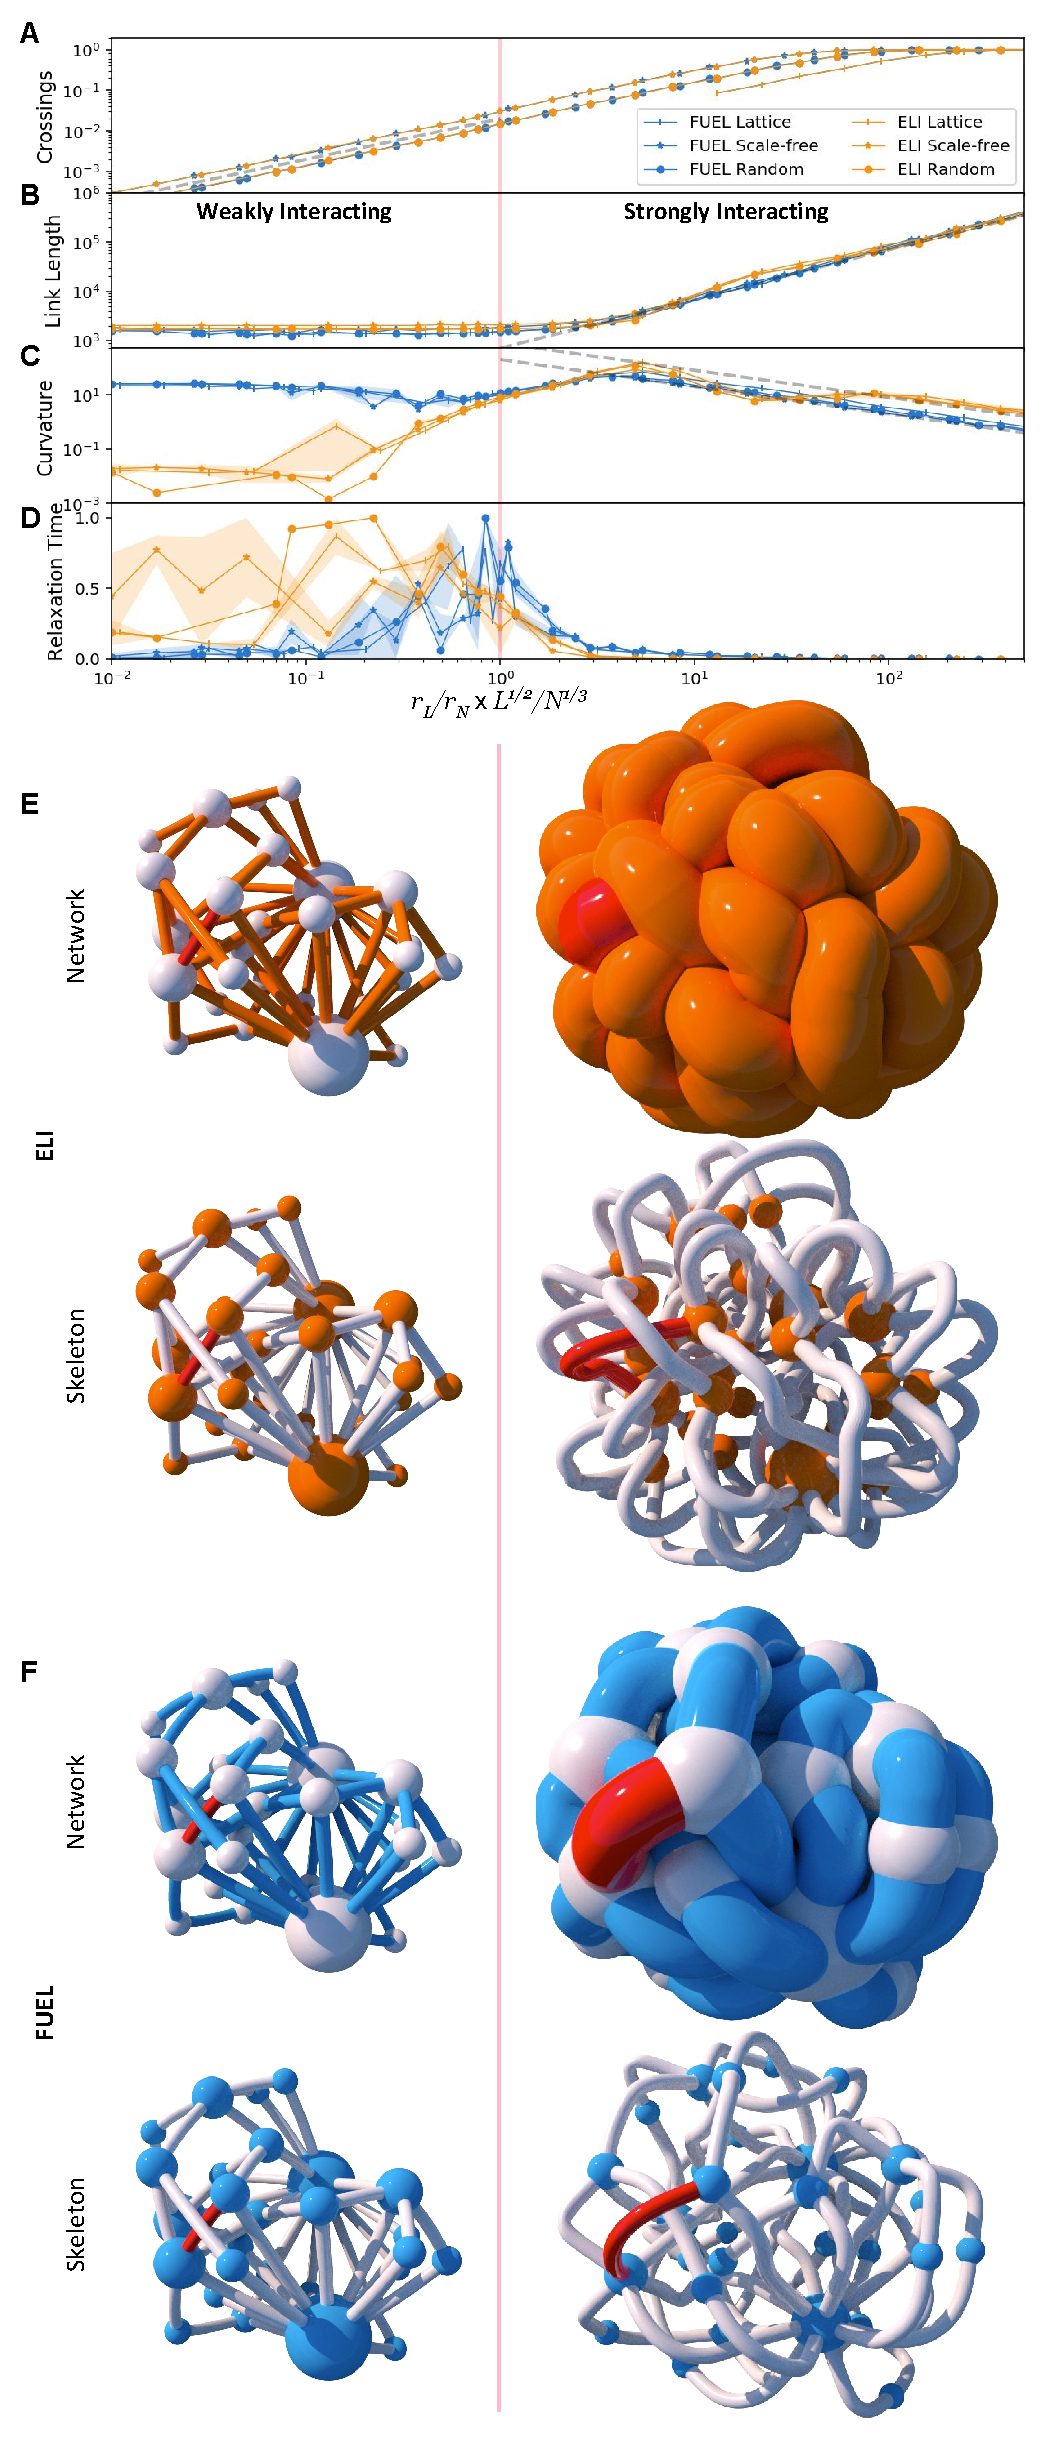
\includegraphics[height=\textheight
% %width=.75\columnwidth
% ]{fig-09-19/3d-phase-compare-103117.pdf}
% 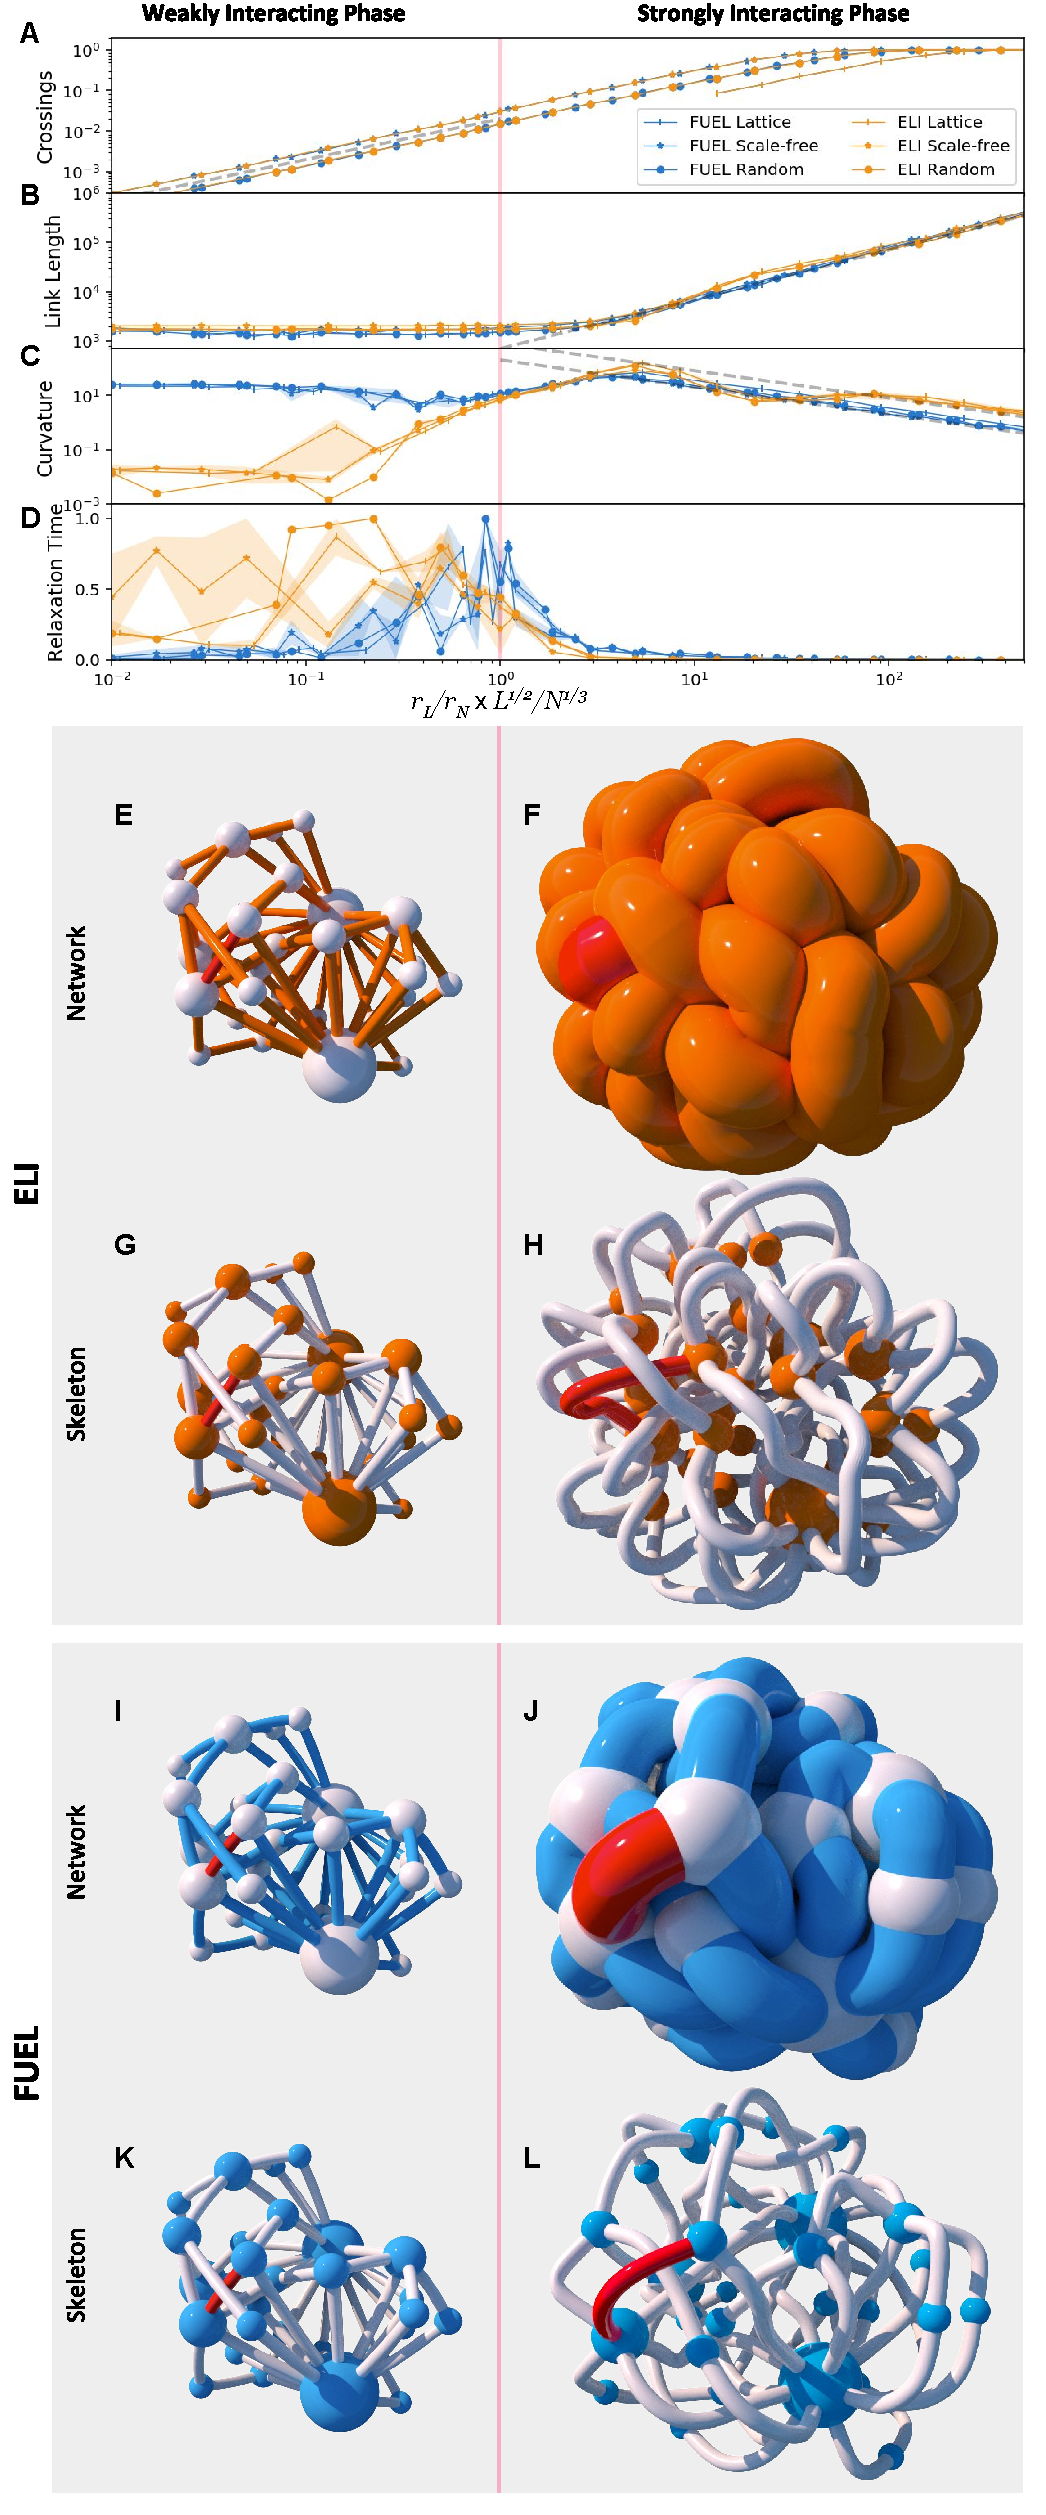
\includegraphics[height=\textheight]{fig-09-19/3d-phase-compare-110317-1.pdf}
%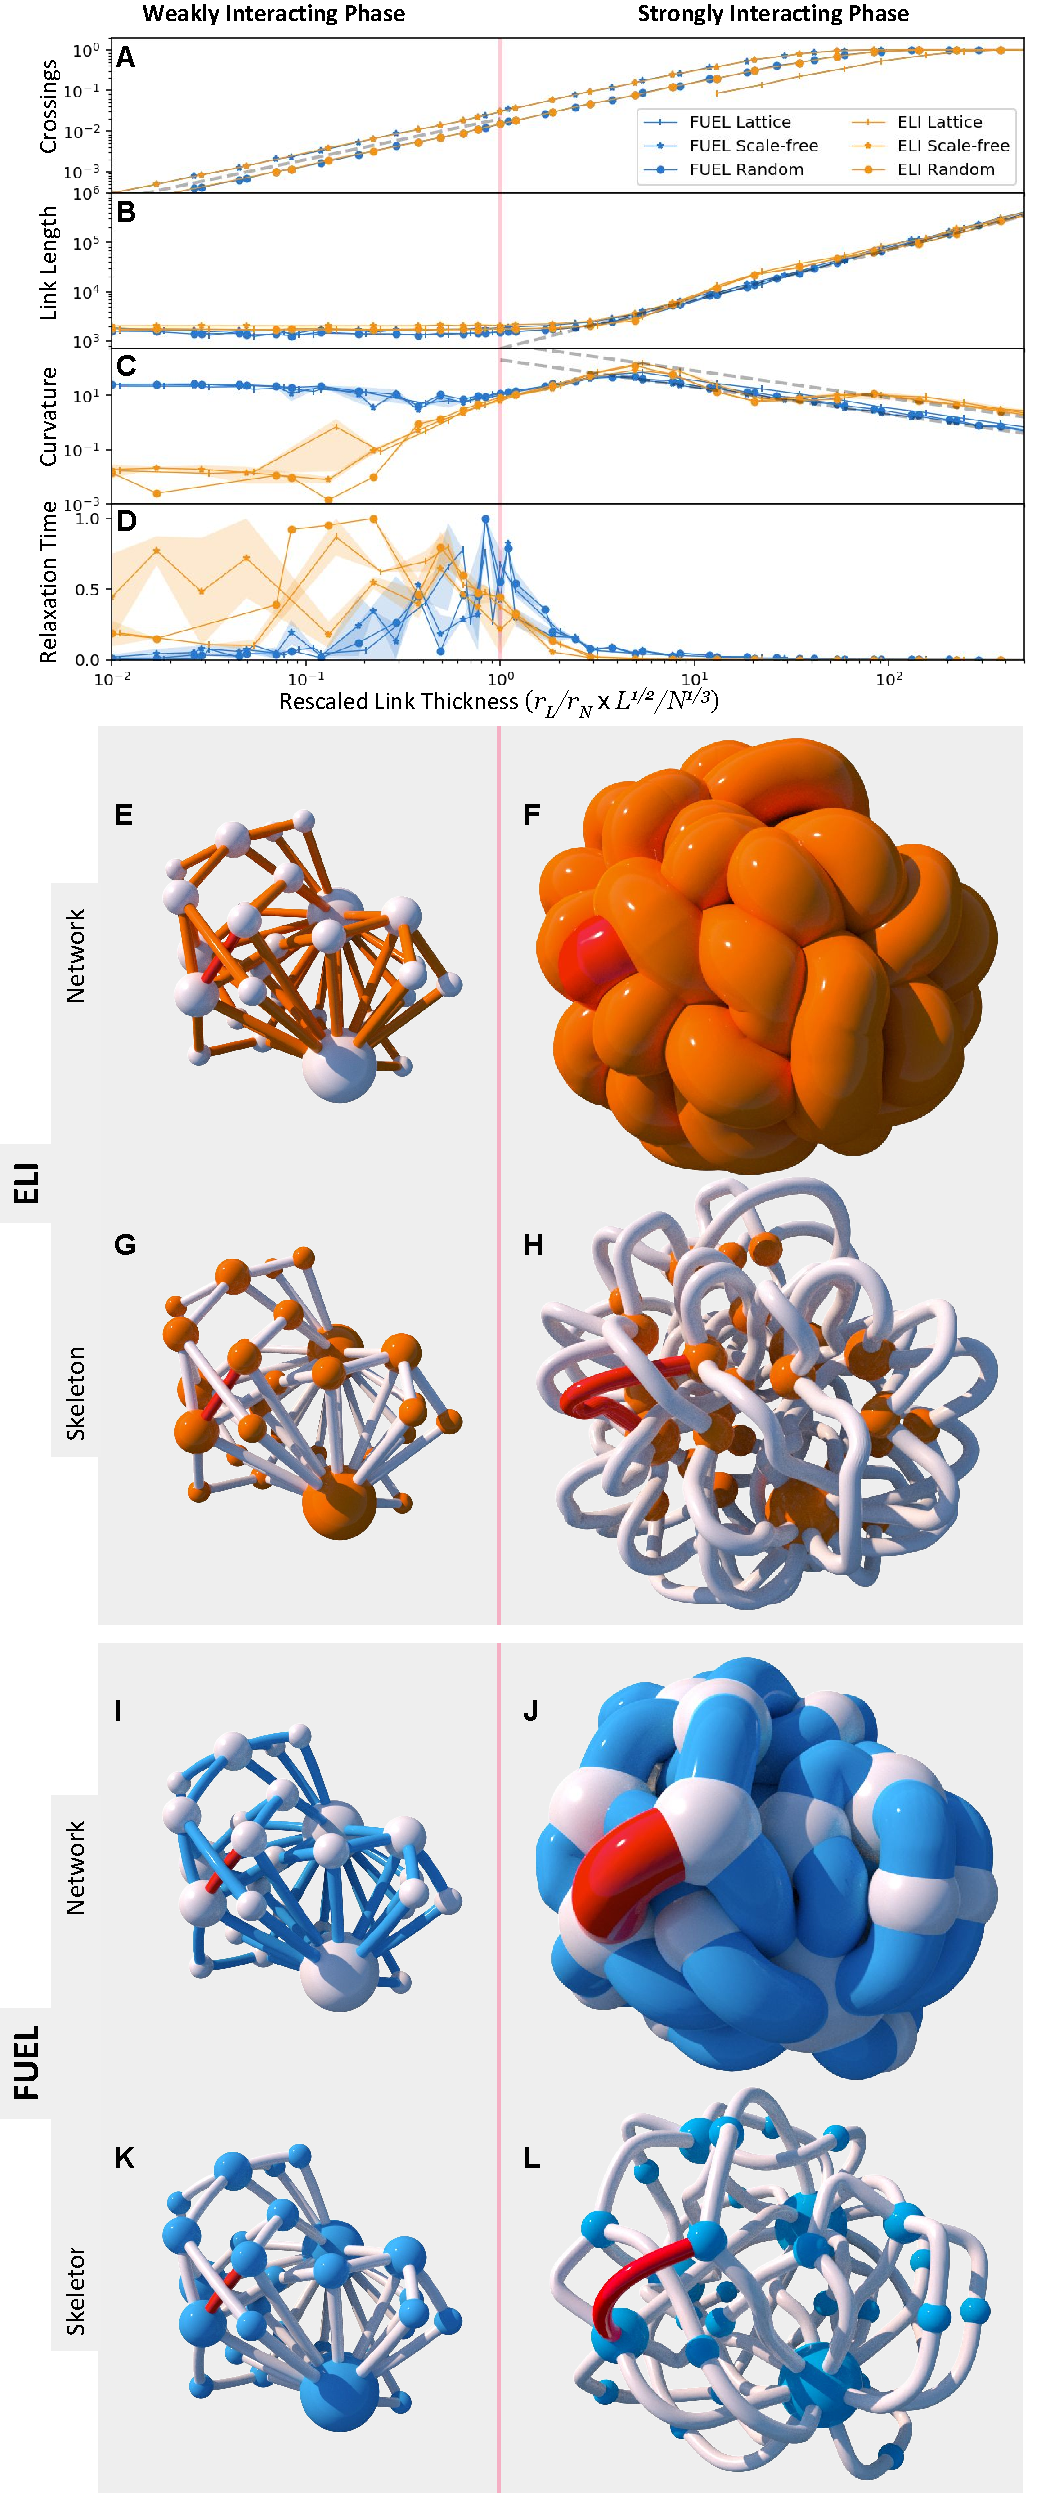
\includegraphics[height=\textheight]{fig-09-19/3d-phase-compare-111917.pdf}
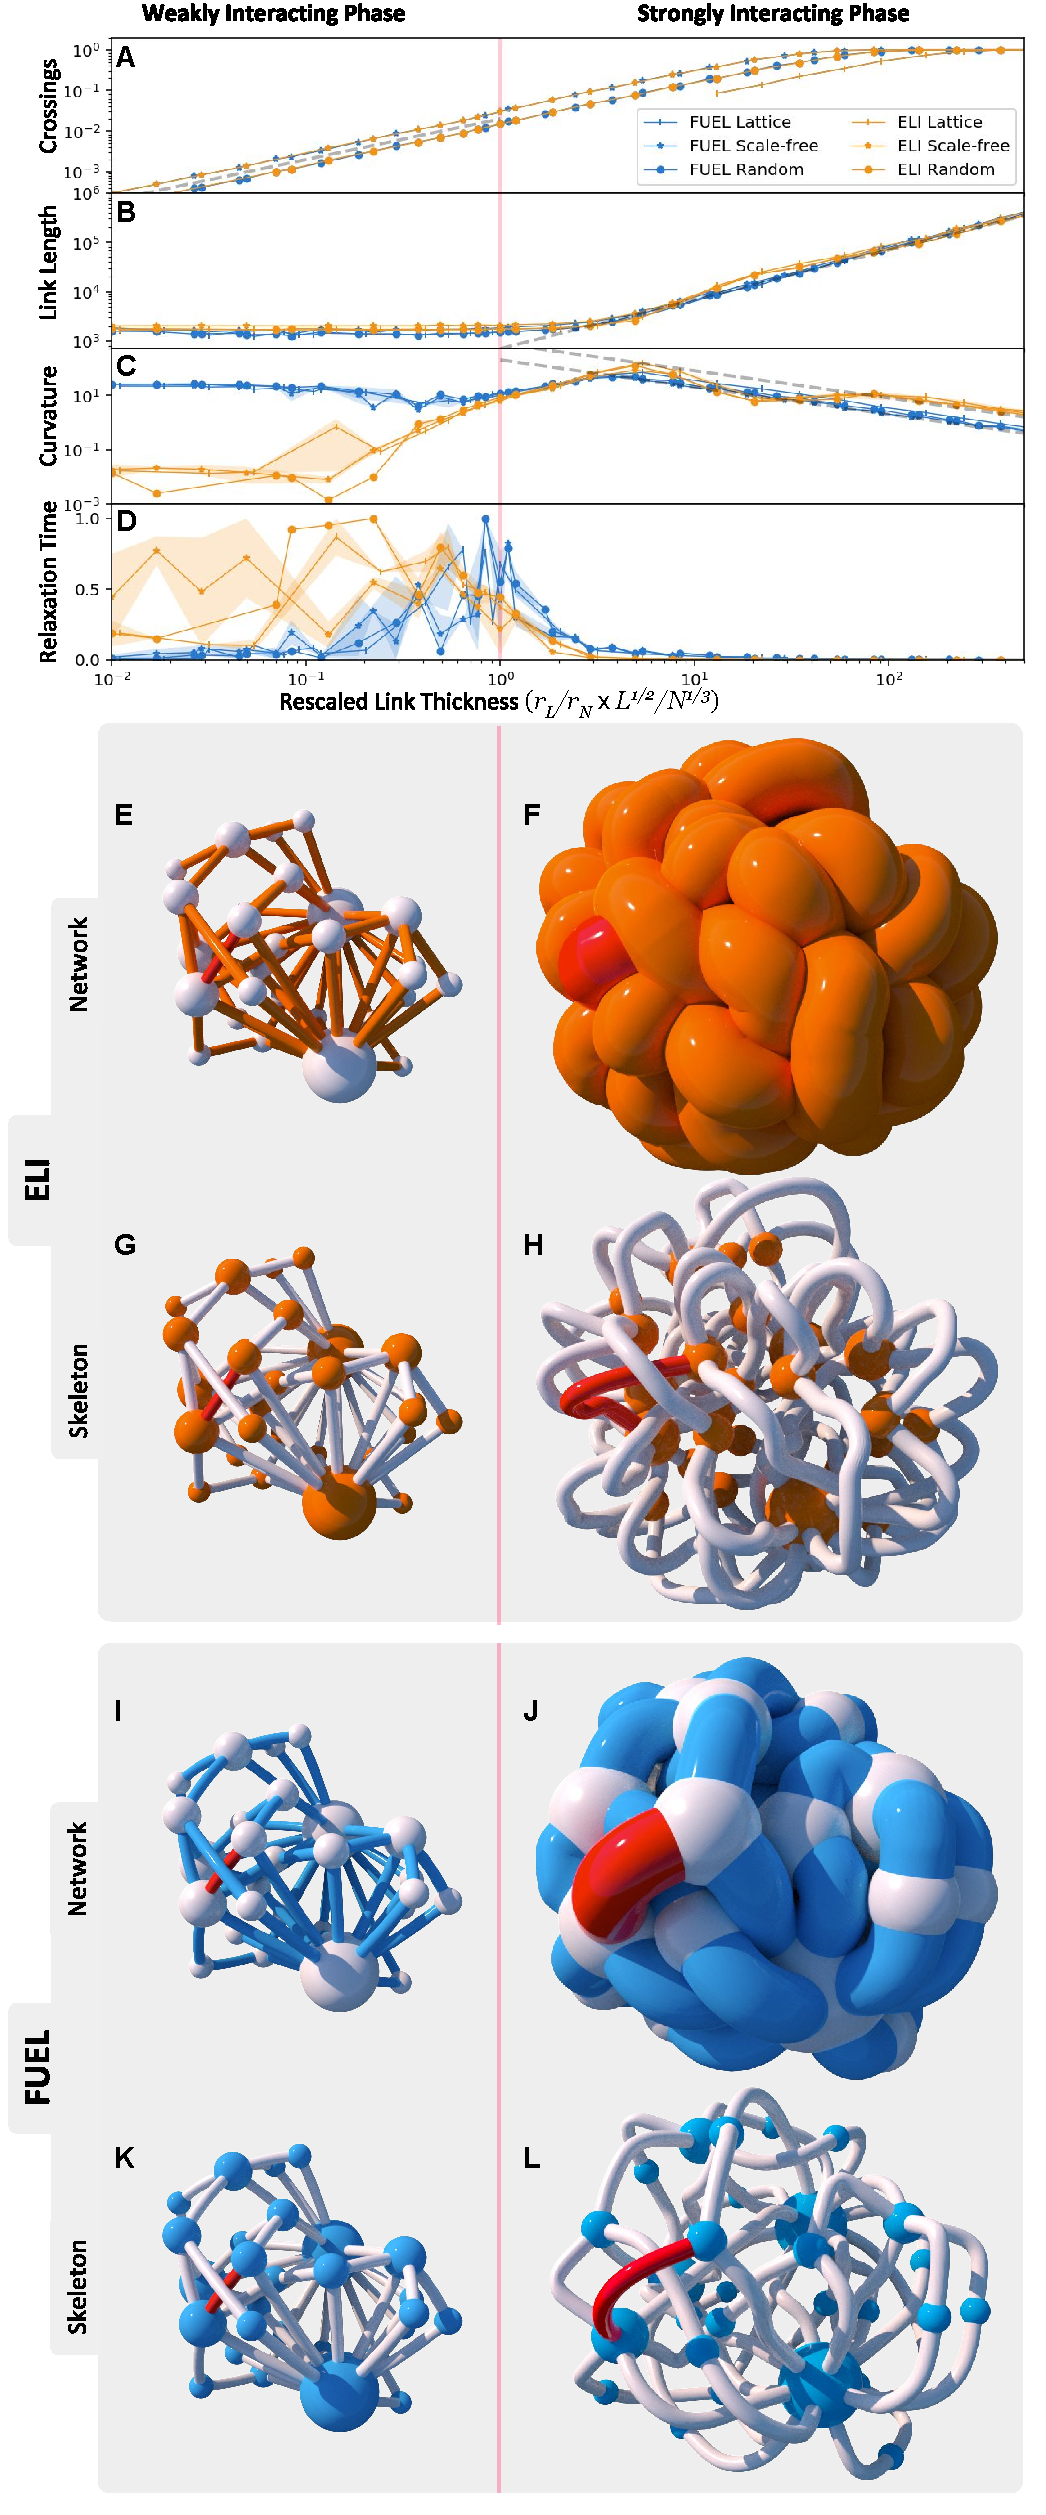
\includegraphics[height=\textheight]{fig-09-19/3d-phase-compare-111917-2.pdf}
\caption{%3D layouts  using ELM and E-ELM, and their phase diagram.
    \scriptsize {\bf Layout Transitions in Networks:} %{\bf (A)} 
    ({\bf A}) The number of crossings in FDL normalized by total number of link pairs grows linearly with the link thickness, saturating only at very high link thickness. 
    A proper layout must resolve an increasing number of local conflicts.    ({\bf B}) The average link length remains largely constant in the weakly interacting regime, but grows linearly in the strongly interacting regime for all topologies and models.
    ({\bf C}) The average link curvature remains fairly constant in the weakly interacting regime, but falls linearly in the strongly interacting regime. 
    Once scaled by the link length, $\be{C}$ is constant in the strongly interacting regime. 
    ({\bf D}) The relaxation time of the simulations indicates a divergence similar to that observed in second order phase transitions. 
    The relaxation times have been scaled by their maximum value for each network topology to help compare the curves.
    The ELI and FUEL geometries: 
    ELI ({\bf E, F}, orange) and FUEL ({\bf I, J}, blue) layout for a BA network \cite{barabasi1999emergence} with $N=20, m=2$. 
    At small thicknesses, $r_L \ll r_N$, both ELI ({\bf E}) and FUEL ({\bf I}) layouts are the similar to FDL. 
    At larger $r_L$ in ELI links bend to avoid each other. 
    The skeleton of ELI ({\bf G} and {\bf H}), where the links are made thin, show that while in the weakly interacting case the links take mostly straight paths ({\bf G}), in the strongly interacting phase links become highly curved ({\bf H}).
    At large $r_L$, links don't fit inside the region containing the nodes and start making outward arcs. 
    ({\bf J}) FUEL at large $r_L$ behaves more gently than ELI ({\bf F}). 
    This can also be seen in the FUEL skeleton ({\bf L}) in the strongly interacting regime, displaying smaller curvatures than ELI ({\bf H}). 
    %and the layout size just grows linearly with the $r$.
    We highlight in each network one link in red to illustrate the change in link trajectories with increasing link thickness.
    The gray line in {\bf B} shows linear increase with $r_L$ and the gray dashed lines in {\bf C} show a $1/r_L$ trend. 
          }    
    \label{fig:phase-compare}
\end{figure}

{\em Weakly Interacting Phase}: For small link thicknesses, $r_L$, the ELI and FUEL layouts are largely indistinguishable from the initial FDL layout.
Indeed, at low $r_L$, the average link length $\be{l}$ is independent of $r_L$ even as the link thickness increases by orders of magnitude (Fig. \ref{fig:phase-compare}B).
This is unexpected, given that there is a tenfold increase in the number of  conflicts (potential link crossings) in this regime (Fig. \ref{fig:phase-compare}A). %
The unchanged $\be{l}$ indicates that ELI and FUEL avoid the increasing number of conflicts by small local bending of the links, without the need to noticeably alter $\be{l}$.
A similar behavior is seen for the average curvature of the links, $\be{C}$, finding that it remains unchanged throughout the weakly interacting phase, indicating that despite multiple local bending necessary to avoid conflicts the links remain largely straight. 
Altogether, we find that in the weakly interacting phase local link rearrangements are sufficient to solve the multiple conflicts FDL suffers from. 

{\em Strongly Interacting Phase}: Once  $r_L$ exceeds a critical value, $r_L^c$, we observe a dramatic change in the layout geometry (Fig. \ref{fig:phase-compare}F, J). 
In ELI, with fixed node positions, the links must take long convoluted routes outside the network to reach their end-nodes, as they are unable to find sufficient empty space between the nodes.  
This change in the link structure is particularly visible on the skeleton of the layout (Fig. \ref{fig:phase-compare}G, H).
In FUEL, with flexible node positions, the links reach their destination by pushing the nodes away from each other. 
These changes alter the behavior of $\be{l}$, which in the strongly interacting phase increases linearly with $r_L$,  
%In other words, local bending cannot resolve the conflicts any longer, hence the links are forced to systematically increase their length to avoid each other. 
and induce rapid changes in the average curvature, $\be{C}$,  at $r^c_L$. %, reflecting the emergence of systematically curved links for large $r_L$. 
After the transition, the curvature decreases as $1/r_L$. 
It is remarkable, however, that despite the different mechanisms the two models employ, and the visually striking differences in the obtained layouts, the scaling of $\be{l}$ and $\be{C}$ in the strongly interacting phase in ELI and FUEL is largely indistinguishable. 
The observed linear increase in $\be{l}$ and the $1/r_L$ decrease in $\be{C}$ is consistent with isometric scaling, indicating that the layouts in the strongly interacting phase are structurally similar to each other if we rescale them by $r_L$ %and are scaling linearly with the $r_L$. 
%Indeed, rescaling the radius of curvature by the layout size results in a constant value in this phase 
(\ref{ap:curvature}). 
\outNim{ 
% 112017
The existence of a phase transition at $r_c$ is also signalled by
% However, once the radius of curvature is scaled by  $\be{l}$ (SI \ref{ap:curvature}), we find that it becomes constant for all networks in the strongly interacting phase (Fig. \ref{fig:phase-compare}E). 
%This implies that in this phase layouts at different $r_L/r_N$ only differ in size and are otherwise very similar.%  layouts in this phase  
% Together with linear growth of  $\be{l}$  (Fig. \ref{fig:phase-compare}D), this implies that layouts in the strongly interacting regime at different $r_L/r_N$ are similar, once scaled by layout size.
%Examining 
the relaxation time, representing the characteristic time the simulations needs to find an equilibrium solution. The strong peak for FUEL near $r_L^c$ (Fig. \ref{fig:phase-compare}D)
%In FUEL, the relaxation time reaches a peak at the transition
%as would be expected from 
documents a critical slowing down typically observed in systems undergoing a second order phase transition.} 

The origin of the observed transition in the layout geometry is revealed by estimating the critical $r_L^c$.
When the links are much thinner than the node repulsion range  $r_N$, the layout is dominated by the repulsive forces between the nodes. 
Hence, the radius $R$ of the ``bounding sphere'' engulfing all nodes is well approximated by the volume of $N$ closely placed spheres of radius $r_N$, hence $ R^3 \sim Nr_N^3 $ (Fig. \ref{fig:trans}D). 
When the total volume of the links exceeds the volume of the bounding sphere, the links cannot fit within the space between the nodes, forcing a change in the layout.  
For large $r_L$ the layout is dominated by the total link volume, implying that the cross sectional area of the layout $\pi R^2$ must be comparable to the cross section of all links, i.e. $ L r_L^2 \sim R^2$ (Fig. \ref{fig:trans}E). 
The transition between the two layouts corresponds to   $r_L$ when the two estimates for $R$ are comparable, predicting that the critical relative radius  scales as
\begin{equation}
    \tilde{r}_c \equiv {r^c_L\over r_N} \sim N^{1/3} L^{-1/2}. \label{eq:trans}
\end{equation}
This predicts that while networks with different $N$ and $L$ transition at different $r_L^c$ values, if we scale the $r_L^c$ by \eqref{eq:trans} the phase transition occurs near 1 for all networks.
The data collapse of Fig. \ref{fig:trans}G confirms that the transition has its roots in excluded volume interactions: the total link volume is negligible in the weakly interacting regime, but it dominates the layout in the strongly interacting phase.
The fact that networks of rather different topologies (scale-free, random) show similar dependence on $r_L$% (Fig. \ref{fig:phase-compare}D)
, suggests that the transition of Fig. \ref{fig:phase-compare} is universal, independent of the network topology and the degree distribution. 

The observed layout transition also alters the  network's physical properties.
For example, a network's response to external forces is captured by the Cauchy stress tensor $T_{\mu\nu} \equiv \ro_\mu\ro_\nu V$ \cite{irgens2008continuum} (\ref{ap:stress}), which depends on the physical and material properties of nodes and links. 
In the weakly interacting regime the links are largely straight, hence the node terms $V_{NN}$ and $V_{NL}$ dominate the total stress. 
As the nodes are surrounded by a varying number of nodes, the stress does not spread uniformly in all directions, but has shear (off-diagonal) stress components, a common feature of solids.
%In other words, networks in the weakly interacting phase have solid-like properties. 
In the strongly interacting phase the links fill up the space,
hence the link contributions $V_{el}+V_{LL}$  dominate $T_{\mu\nu}$, 
%The adjacent link segments will be at a distance $|x_l-x_m| = \be{r} = 2 r_L$, hence space-filling and uniformity 
resulting in a diagonal total stress tensor (\ref{ap:stress}). 
In other words, we predict that networks in the strongly interacting phase display a fluid or gel-like response to external stress. 
\begin{figure}
    \centering
    %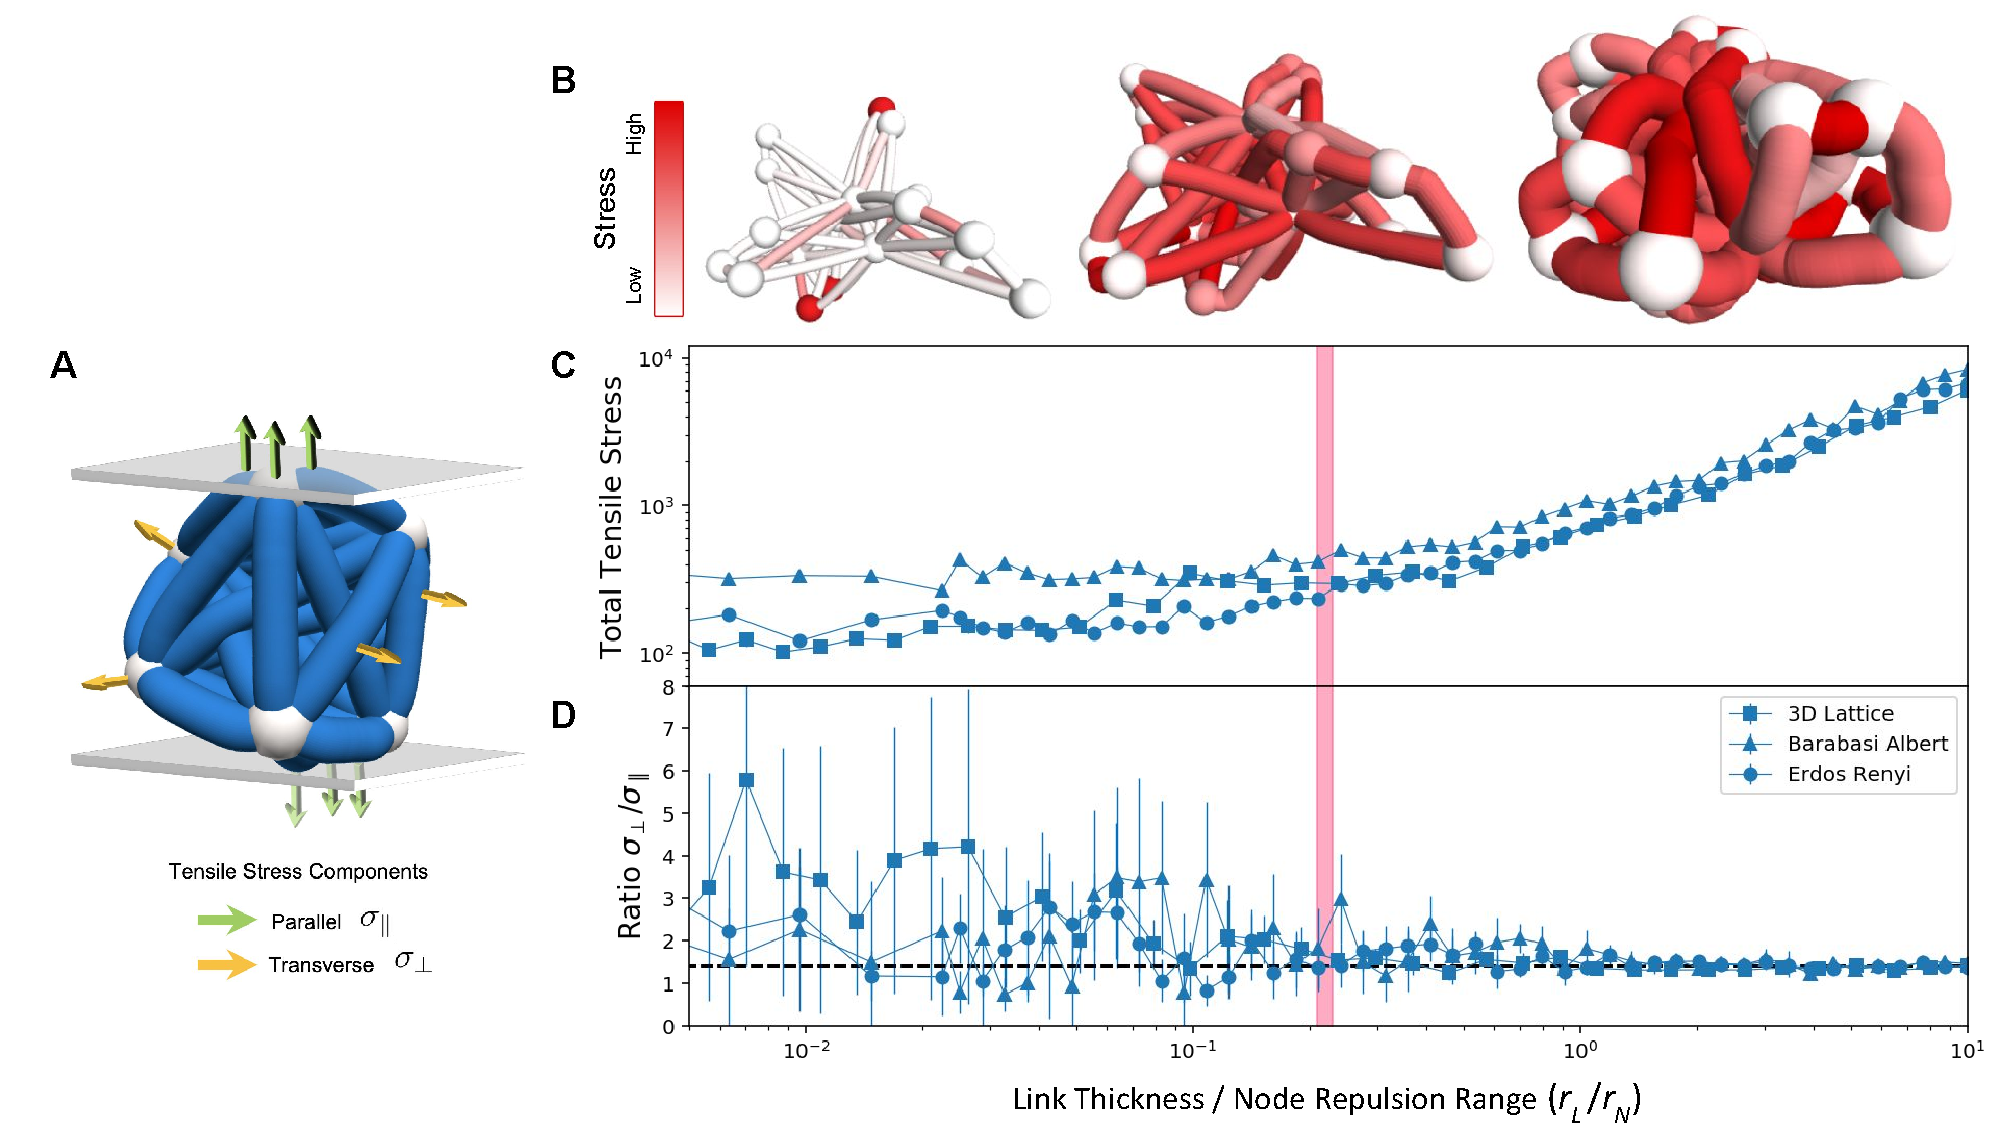
\includegraphics[width=1\columnwidth]{fig-09-19/stress-plots-3.pdf}
    % 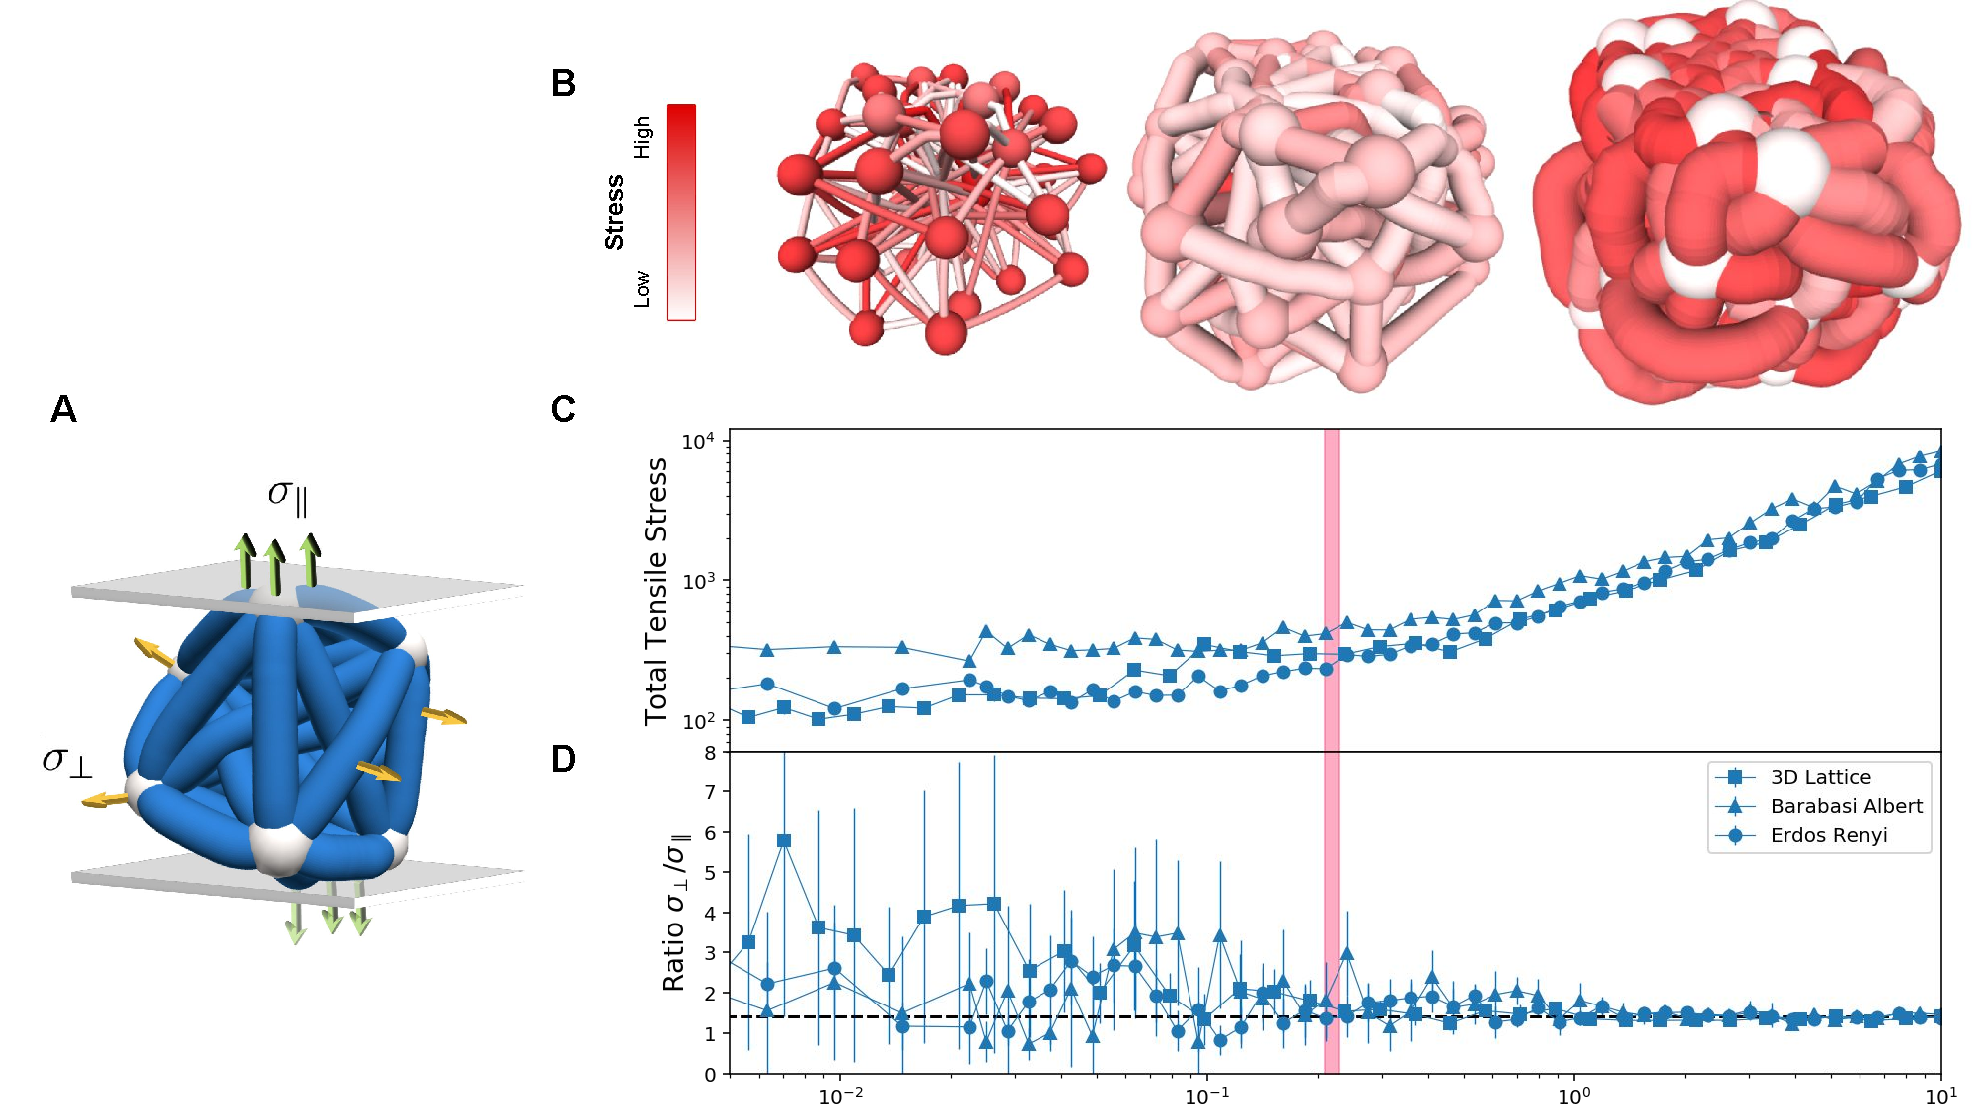
\includegraphics[width=1\columnwidth]{fig-09-19/stress-2.pdf}
    % 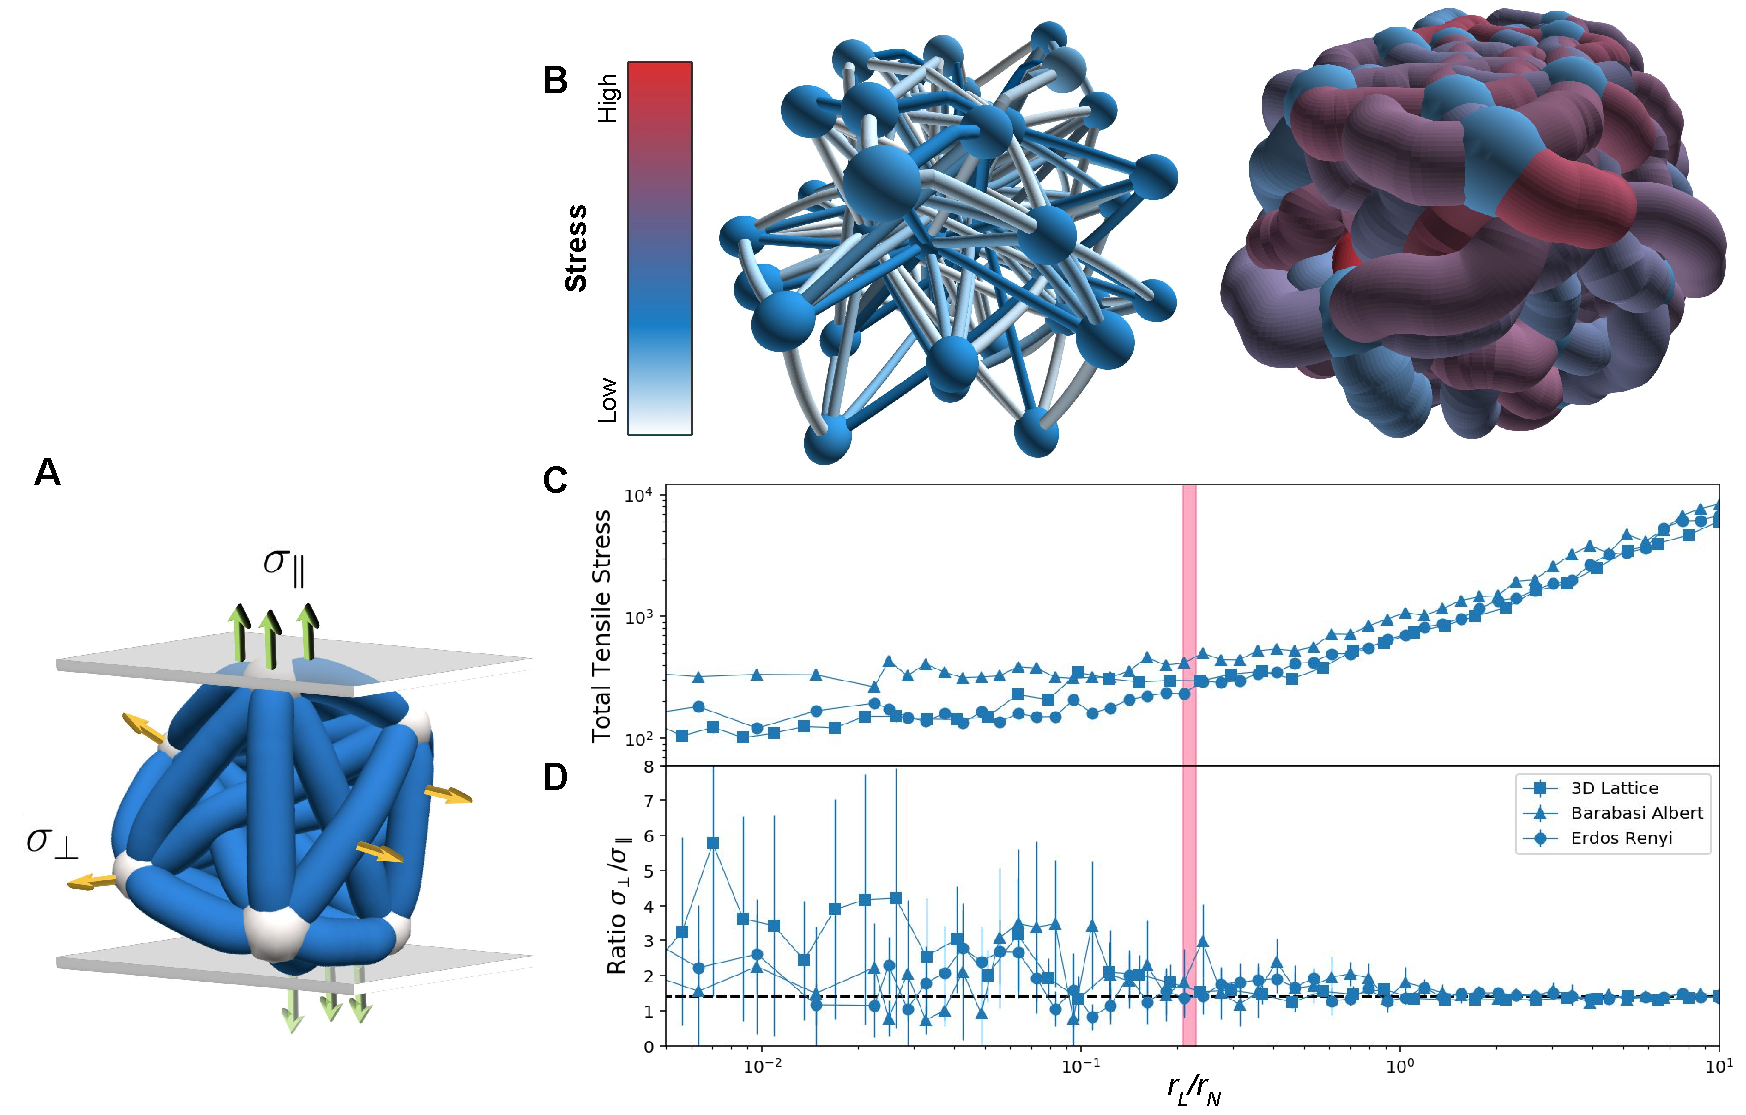
\includegraphics[width=1\columnwidth]{fig-09-19/stress-4.pdf}
    % 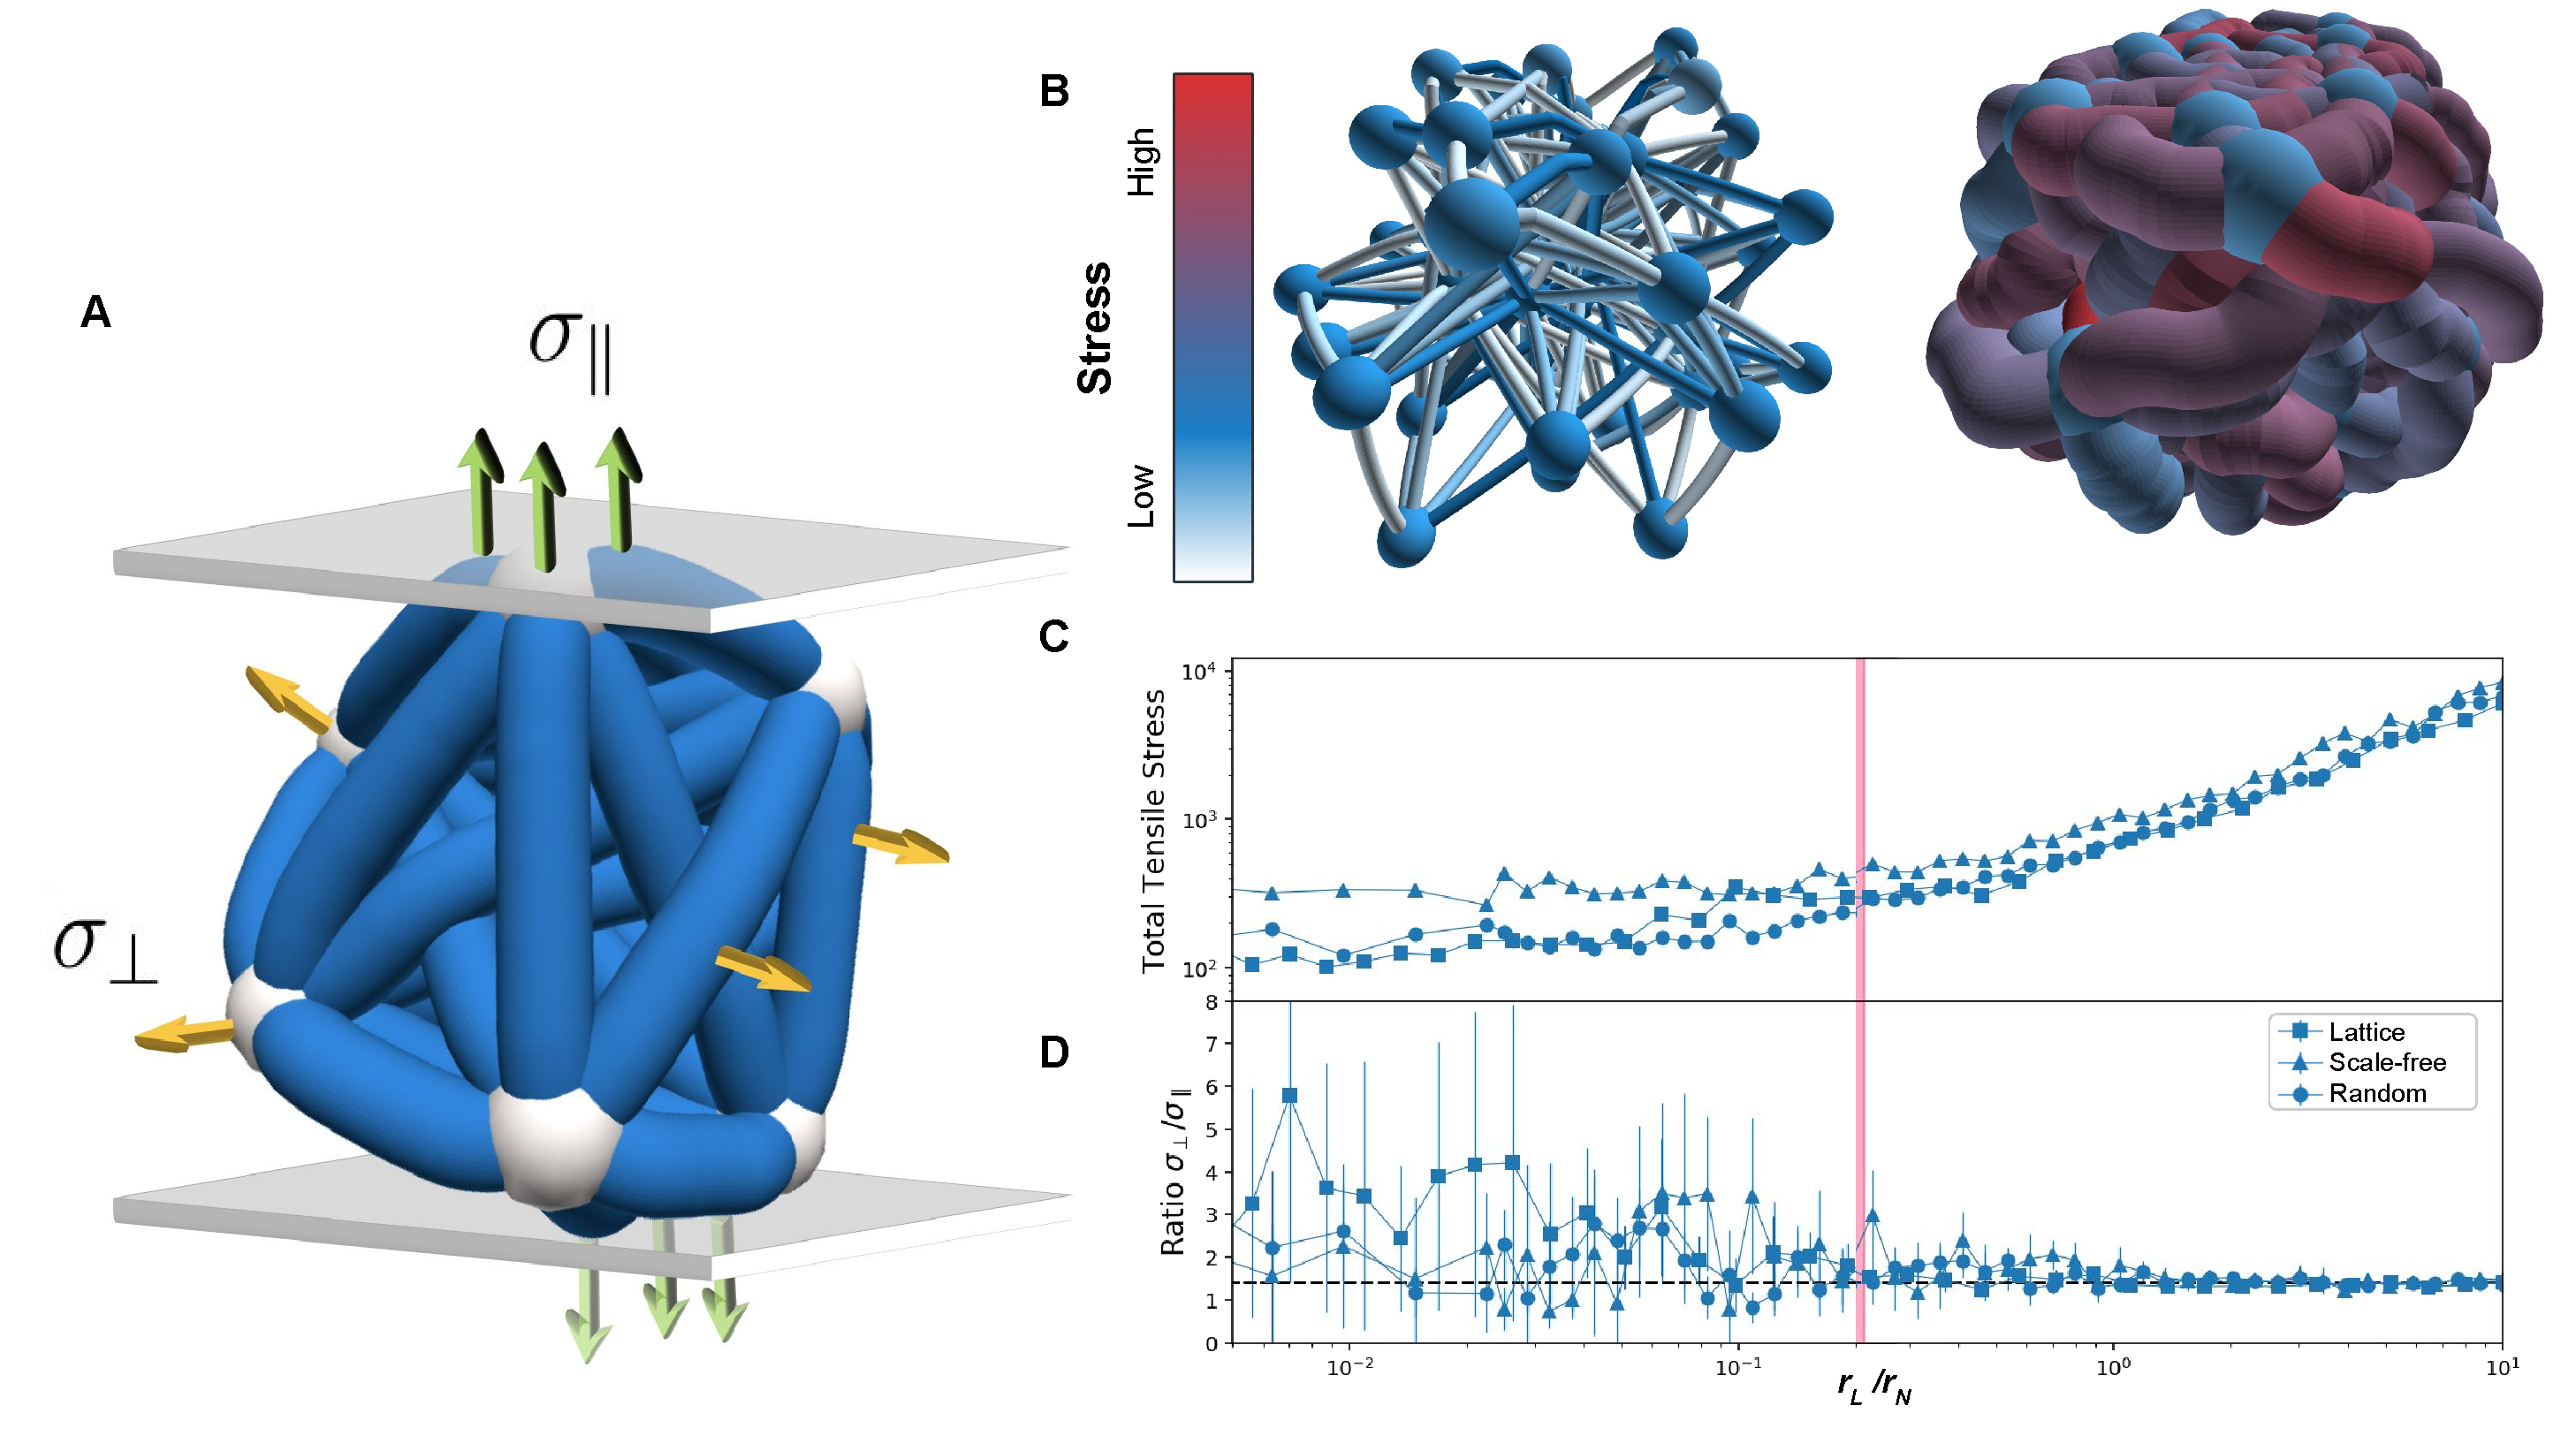
\includegraphics[width=1\columnwidth]{fig-09-19/stress-071917.pdf}
    % 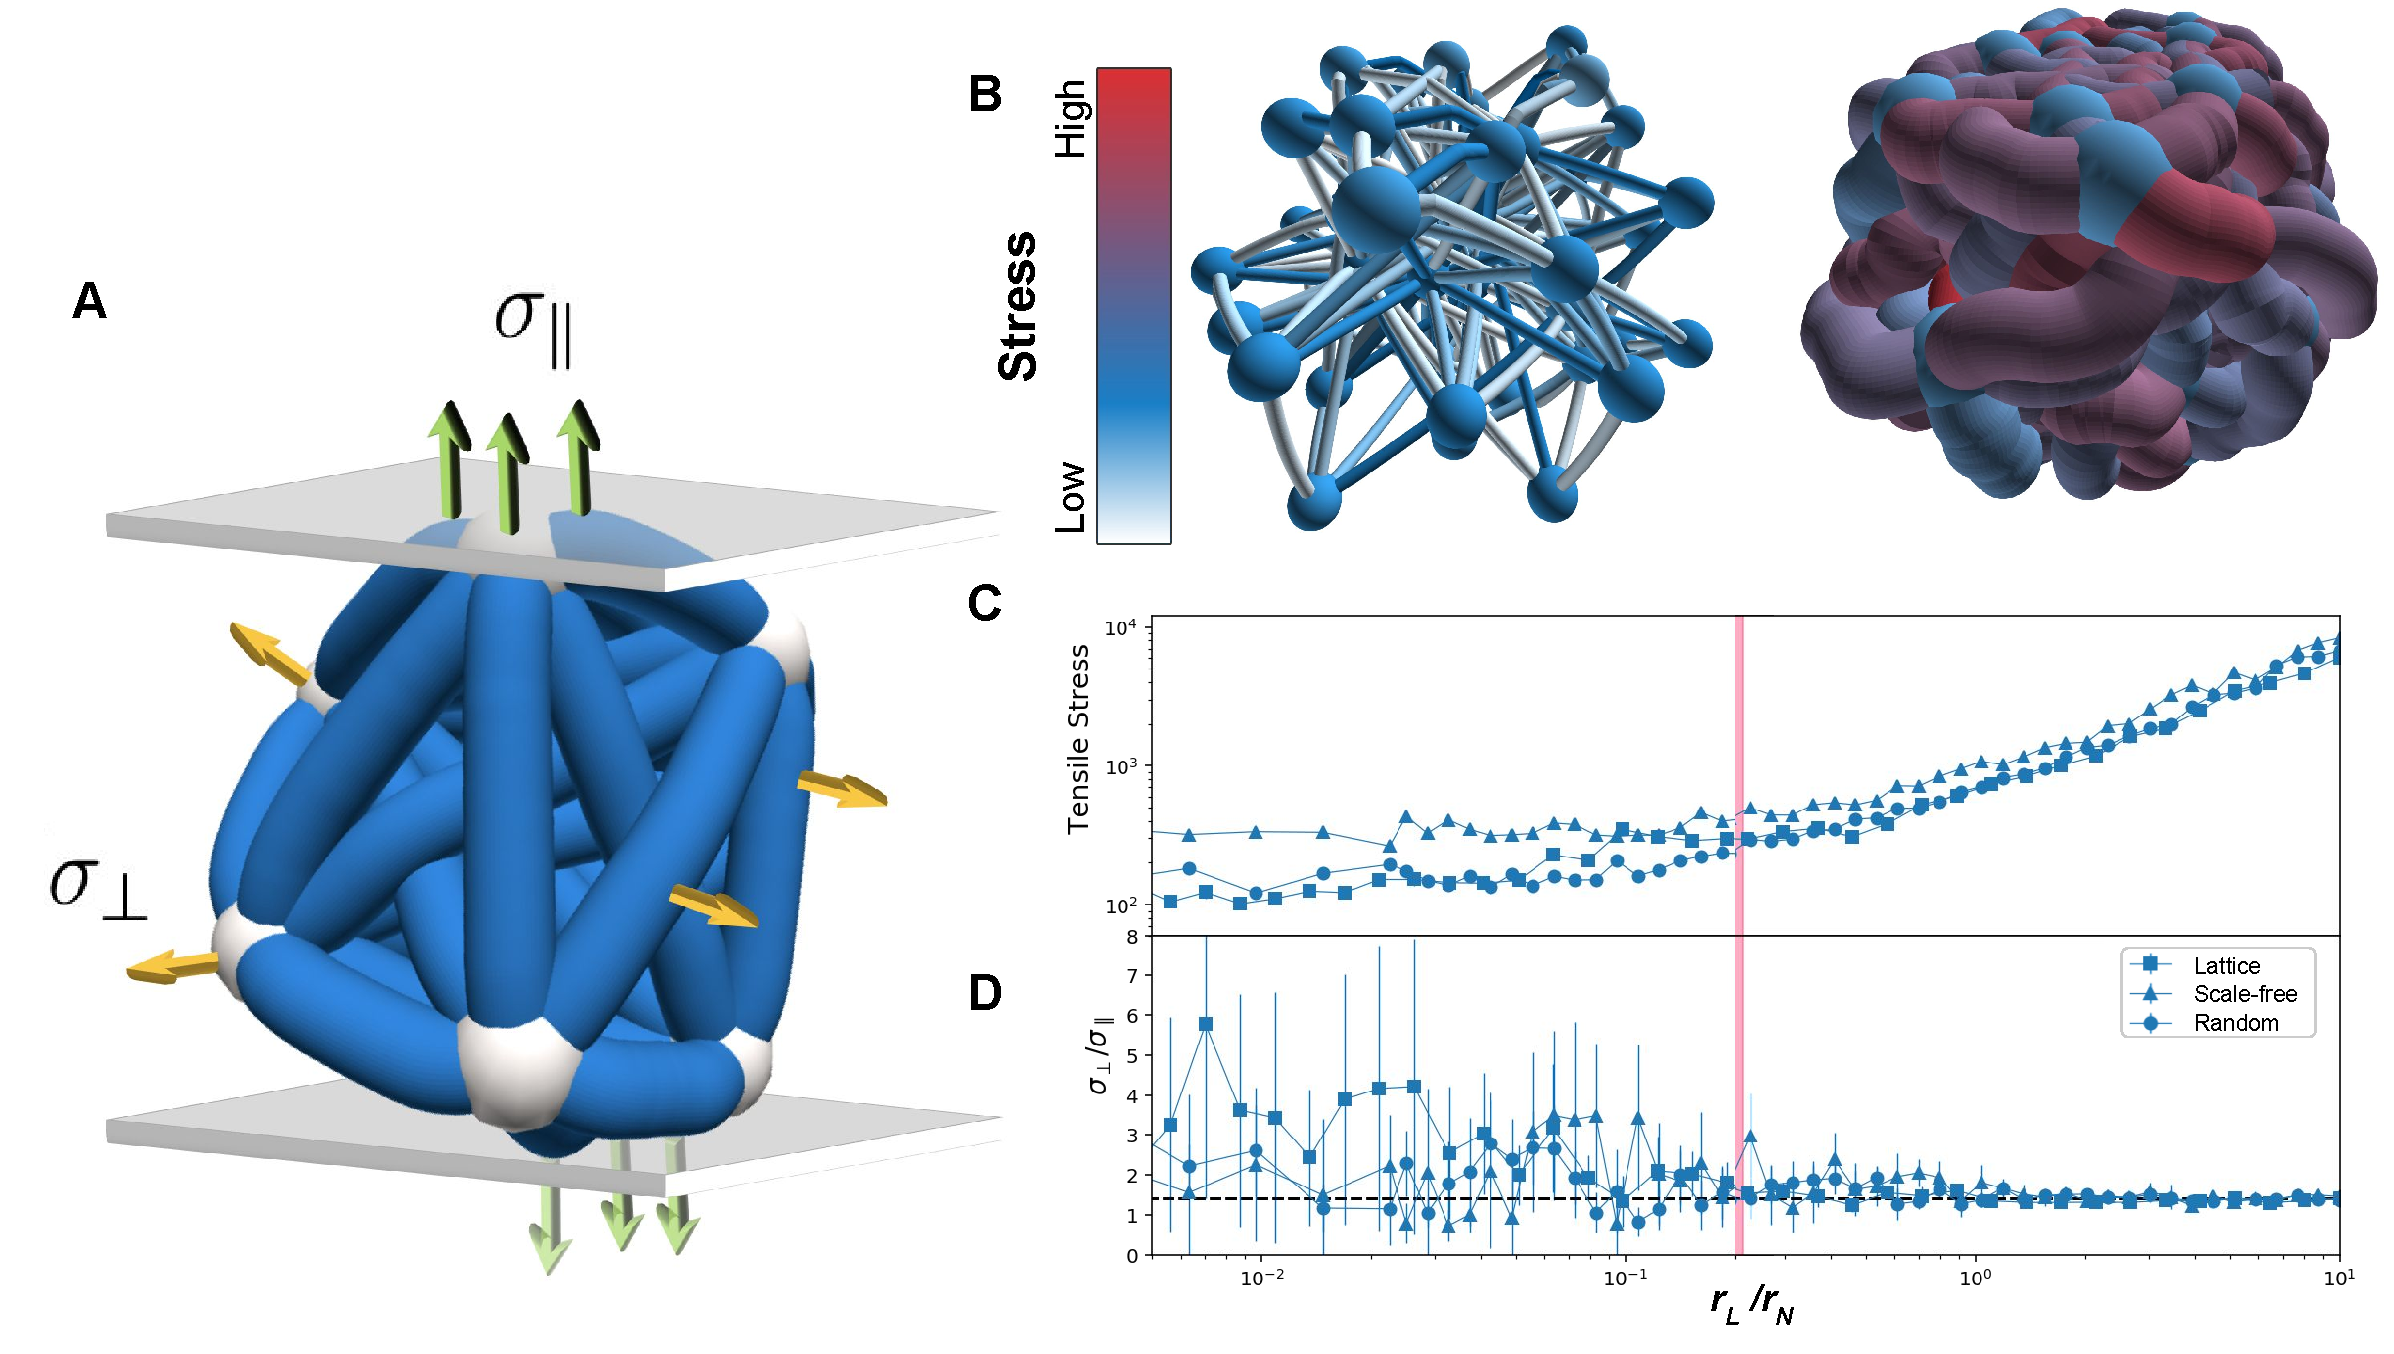
\includegraphics[width=1\columnwidth]{fig-09-19/3D-stress.pdf}
    
    \vspace{5cm}
    % 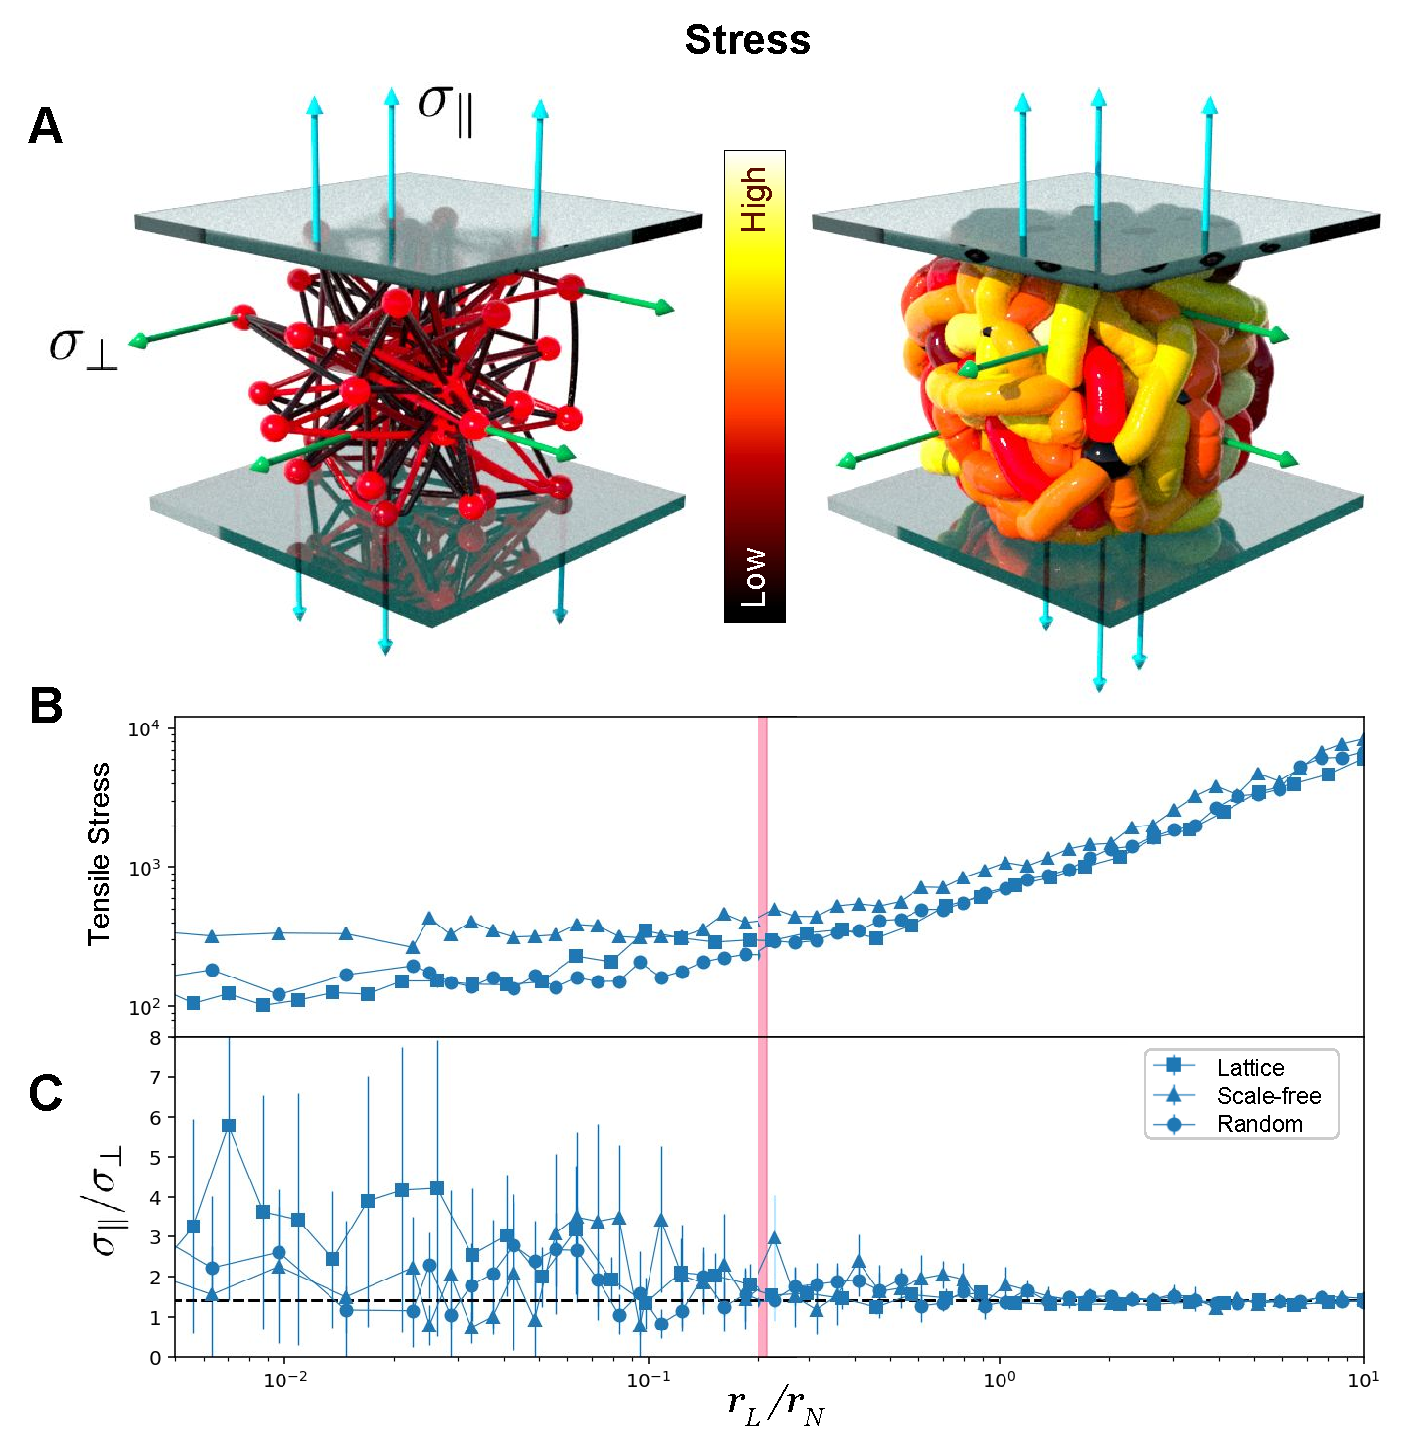
\includegraphics[width=.9\columnwidth]{fig-09-19/3D-stress-101217.pdf}
    %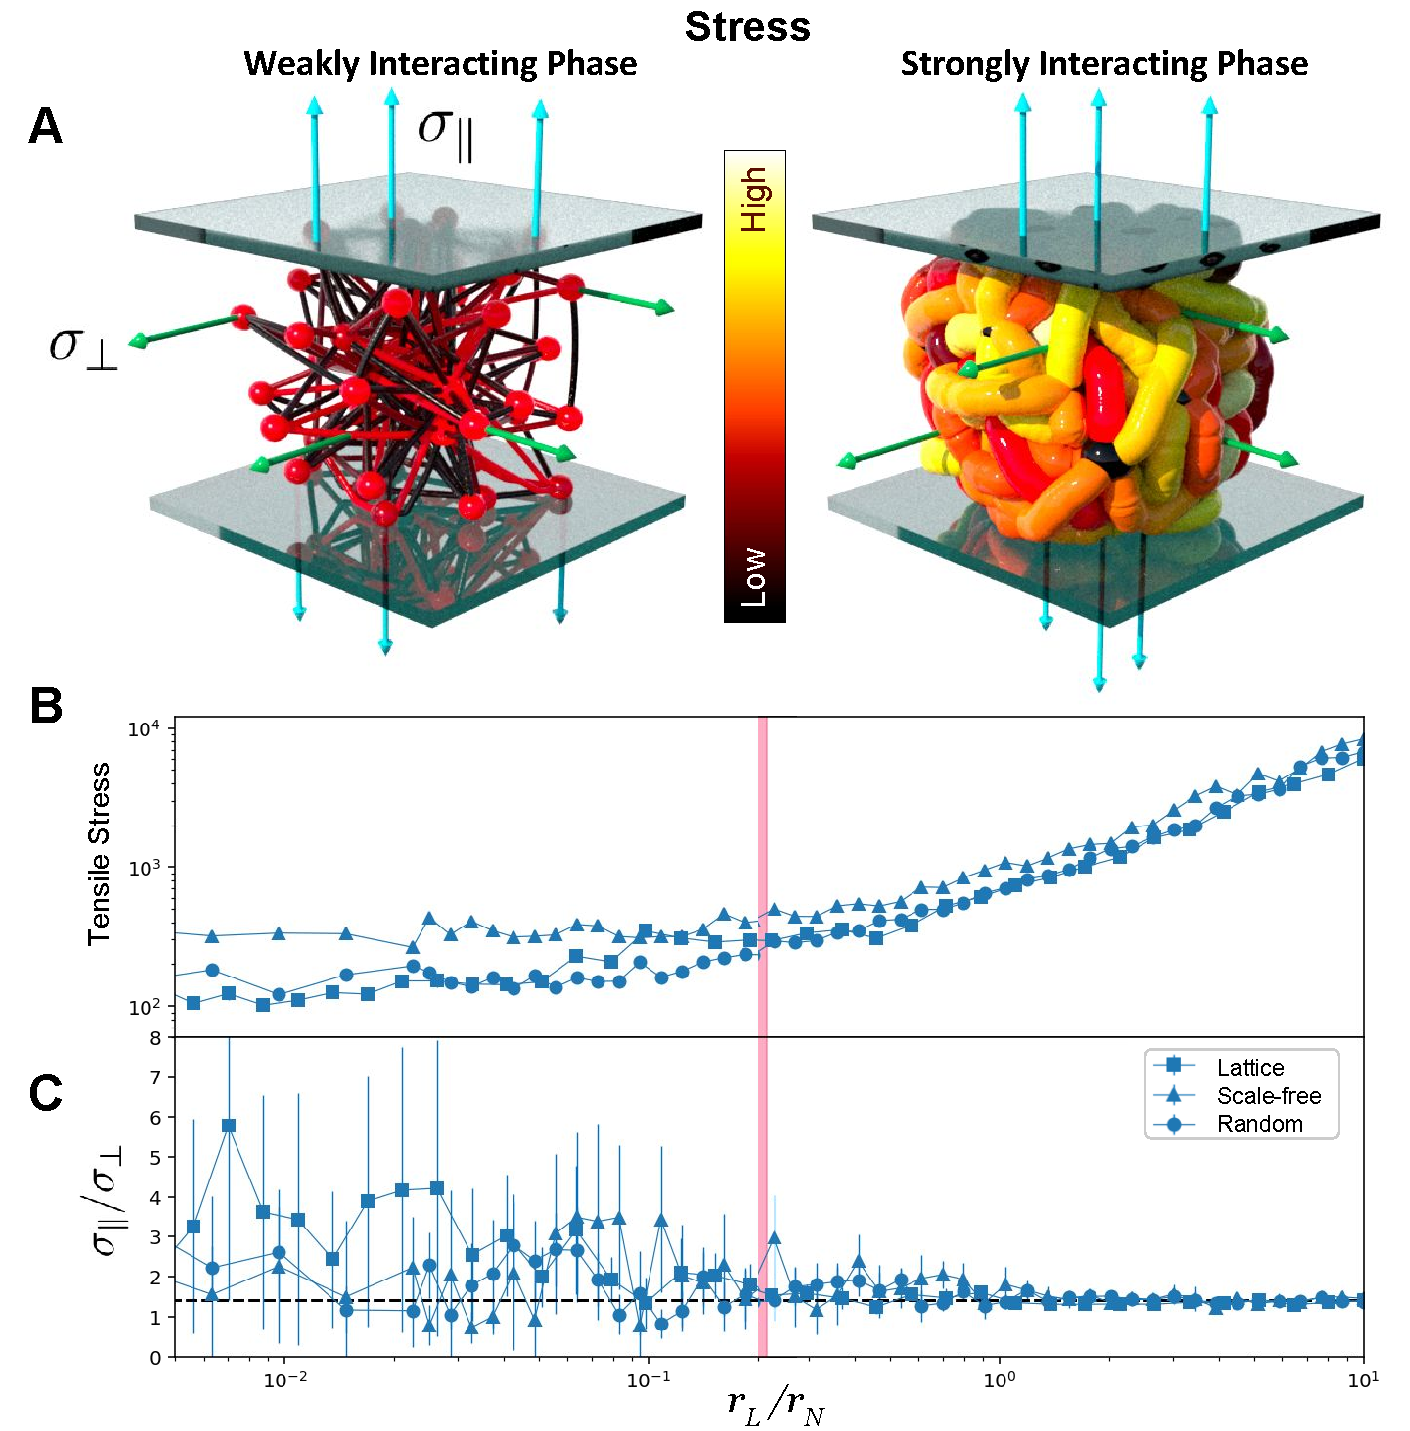
\includegraphics[width=.9\columnwidth]{fig-09-19/3D-stress-110317.pdf}
    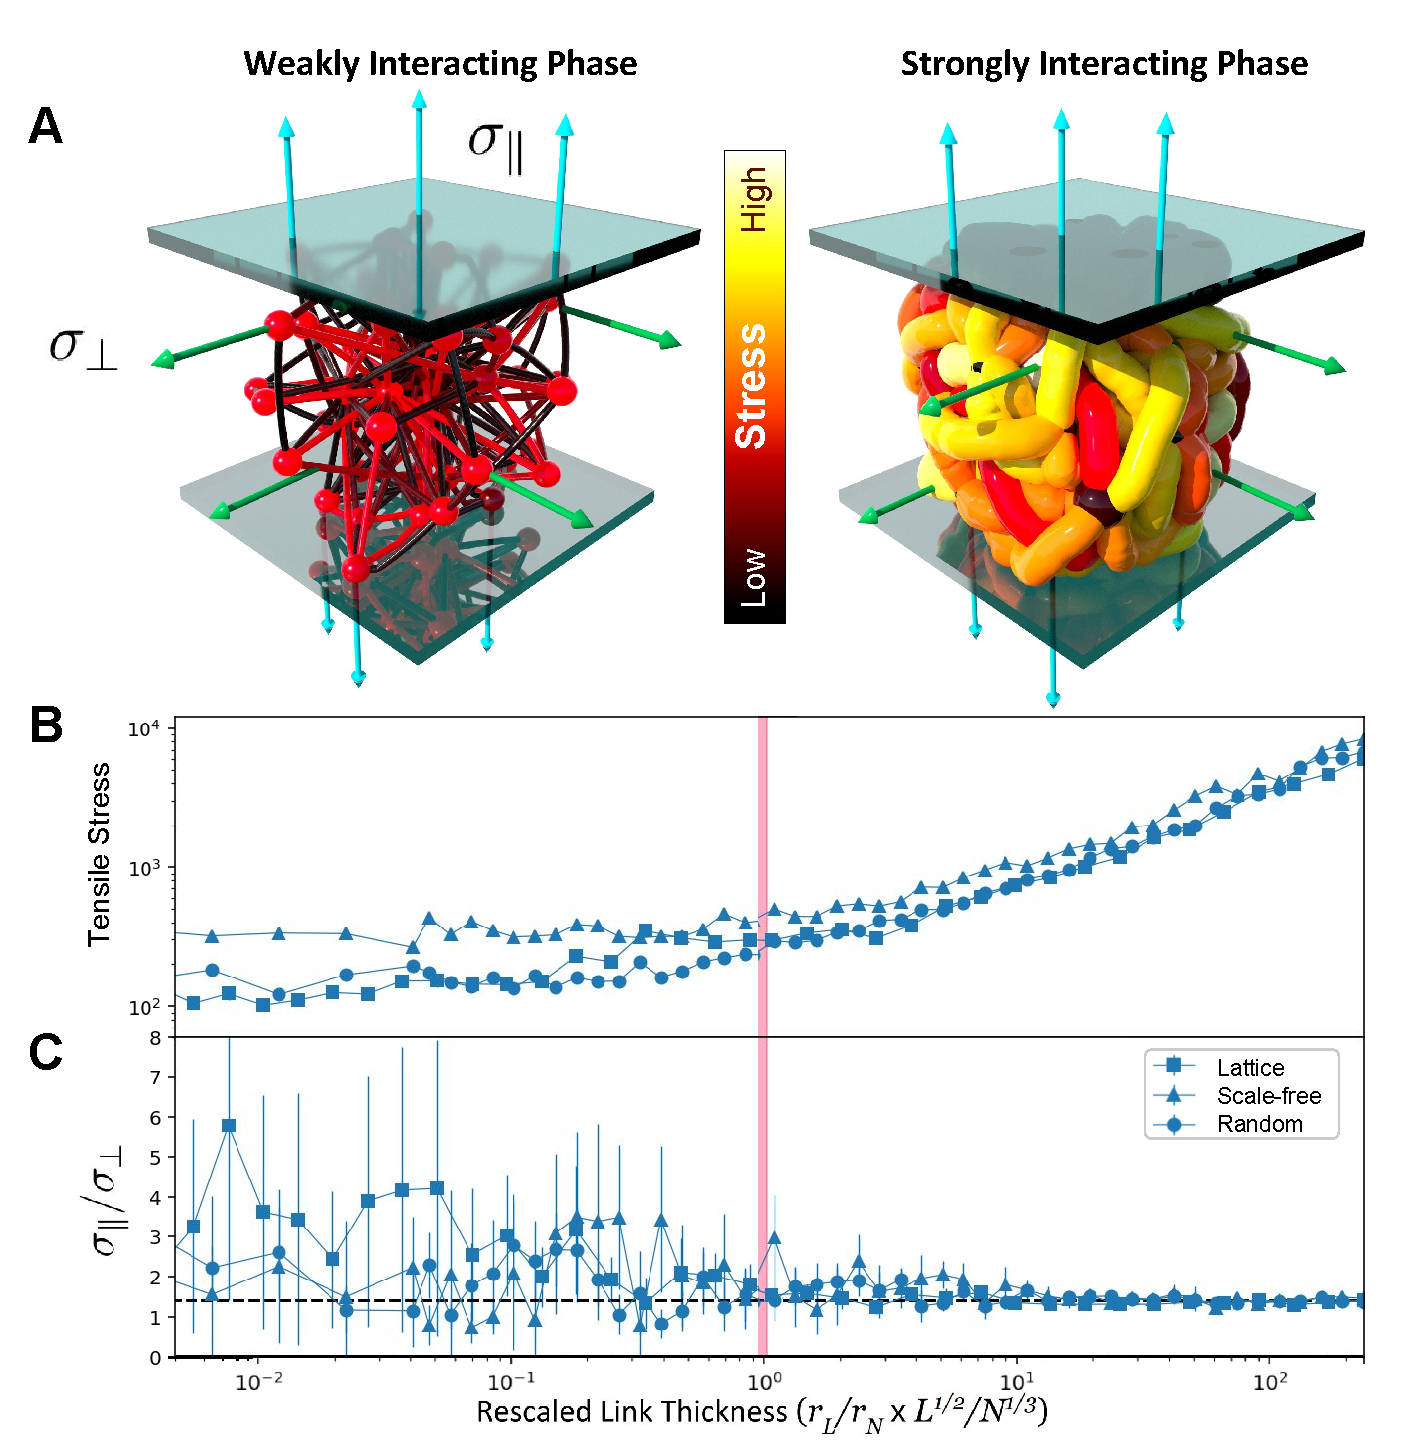
\includegraphics[width=.9\columnwidth]{fig-09-19/3D-stress-111917.pdf}
    \caption{\scriptsize
    {\bf Networks Under Stress: (A)} The tensile stress build-up in the nodes and links as a result of confining a network between two horizontal walls that
    compress it in the vertical direction.
    The cyan arrows show the forces pushing vertically on the walls, i.e. the local tensile stress parallel to the direction of compression ($\sigma_\parallel(x)$). 
    The green arrows indicate the tensile stress $\sigma_\perp(x)$
    perpendicular to the compression. 
    The network on the left and the right are in the weakly and strongly interacting phase, respectively. 
    The nodes and links are colored based on the total amount of stress accumulated in them. 
    %The stress levels go from dark red for very little stress to bright yellow for very high stress. 
    %{\bf (B)} Examples of layouts showing total stress (more red means more stress).  
    %Each network corresponds to the  link thicknesses in the plots below them.
    In the weakly interacting phase (left) the stress is concentrated in the nodes and the stress experienced by the links is small. 
    %Near the phase transition (middle) both nodes and links show a stress, and 
    In the strongly interacting phase (right), almost all the stress is in the links.  
    {\bf (B)} Total stress of different network topologies as a function of link thickness. Since the definition of $x,y,z$ is frame-dependent, we measure the forces for 50 random network orientations. 
    %Because networks are inhomogeneous objects, stress is averaged over 50 random network orientations. 
    The weakly interacting phase shows a slowly increasing level of stress for increasing thicknesses. %, but the value also fluctuates a lot at different orientations (\ref{ap:stress}). 
    At the transition point the trend changes and in the strongly interacting phase stress grows linearly with link thickness. 
    In this phase the stress in the links is larger than stress in the nodes (\ref{ap:stress}). 
    {\bf (C)} The ratio of parallel and transverse tensile stress $\sigma_\perp/\sigma_\parallel$, error bars showing its fluctuations over the 50 random orientations of the layout. 
    In the weakly interacting phase the ratio depends on layout orientation,
    a solid-like feature.
    %where local molecular structure spreads stress in a random manner dependent on the direction of compression. 
    As we transition into the strongly interacting phase, the fluctuations of $\sigma_\perp/\sigma_\parallel$ decay to zero. 
    In this phase we predict $\sigma_\perp/\sigma_\parallel \approx \sqrt{2}$, 
    the value expected in a non-viscous fluid where all three components of tensile stress equal to the pressure.}
    \label{fig:stress}
\end{figure}
\outNim{
\begin{figure}
    \centering
    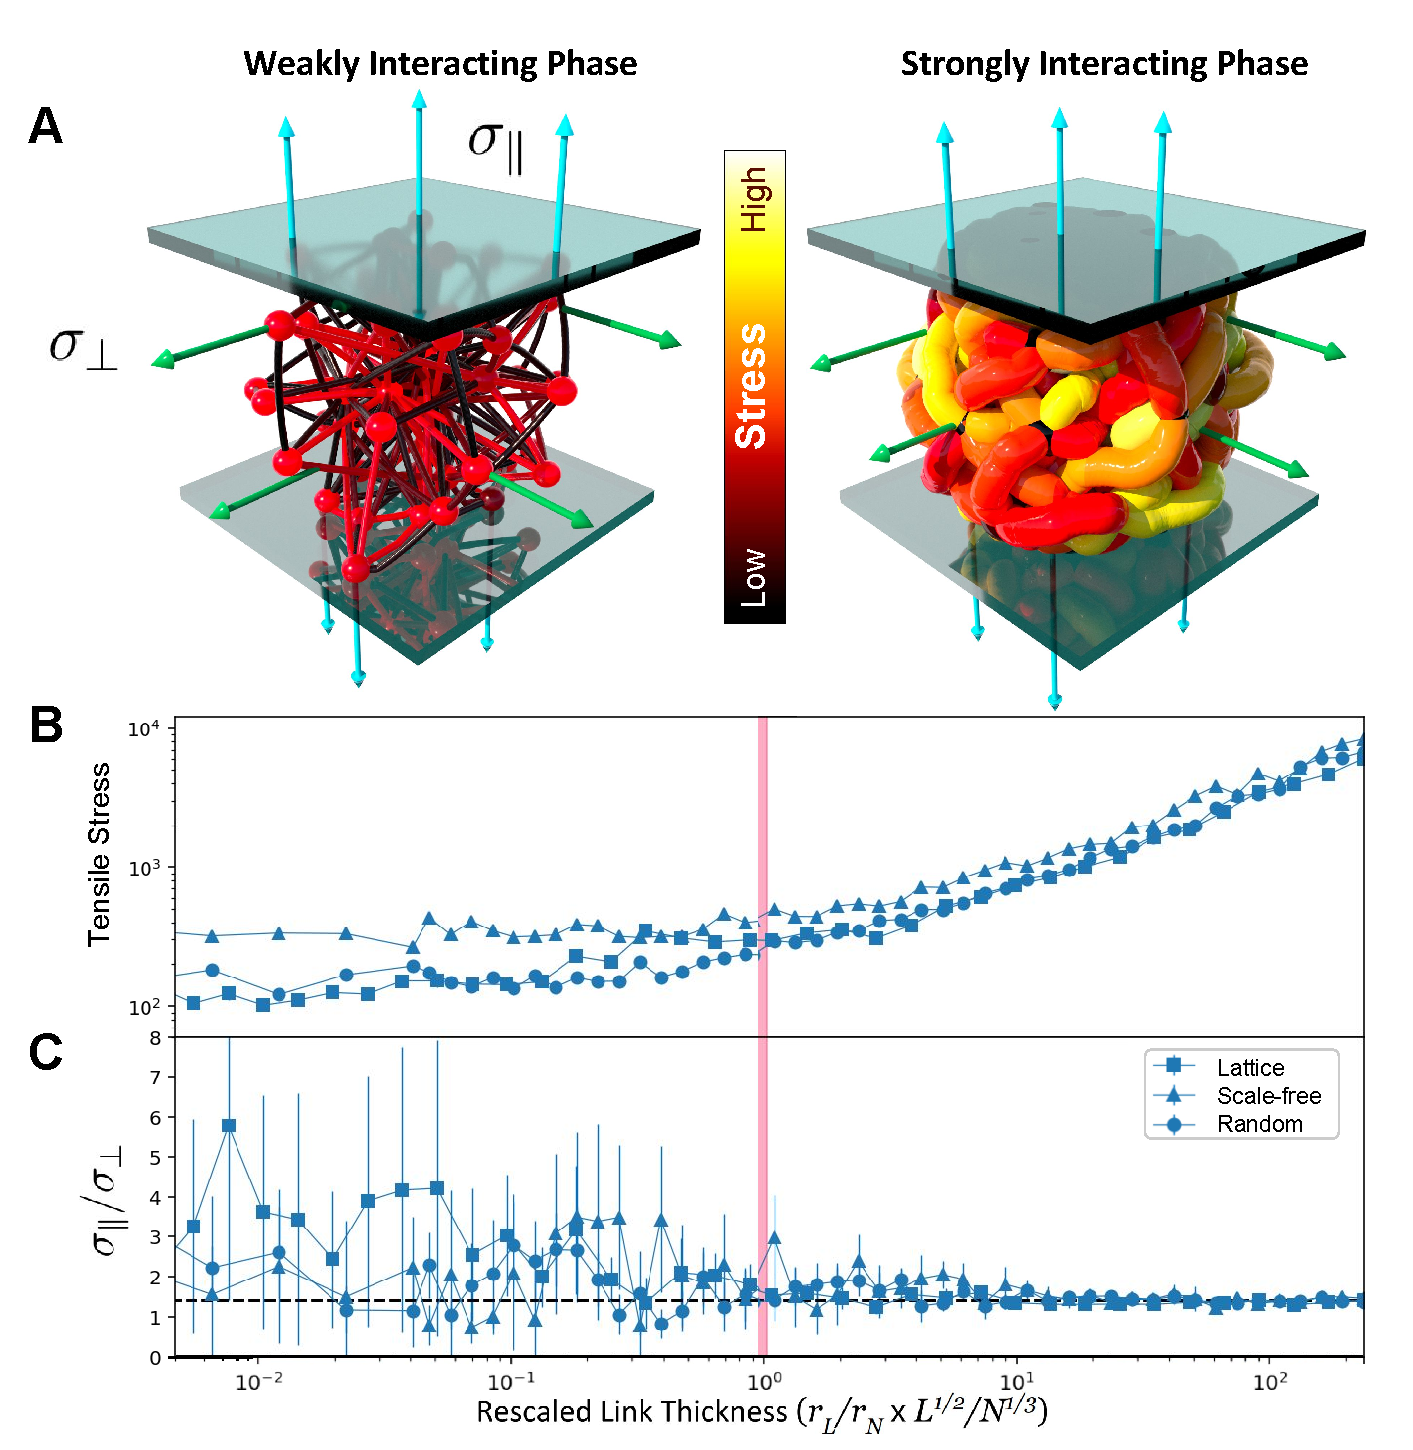
\includegraphics[width=.9\columnwidth]{fig-09-19/3D-stress-111917-1.pdf}
\end{figure}
} %%%%
To test the validity of the predicted solid-gel transition,
we compress the networks generated by FUEL in the $y$ direction and measure the tensile forces 
$ \sigma_\mu \equiv T_{\mu\mu}$ (Fig. \ref{fig:stress}A, \ref{ap:stress}).
We observe a transition at $\tilde{r}_c$ predicted by \eqref{eq:trans} from a roughly constant stress in the weakly interacting regime to a monotonically increasing total stress in the strongly interacting regime (Fig. \ref{fig:stress}B). 
Furthermore, as we rotate the network, we
find that the total stress ratio $ \sigma_\parallel/ \sigma_\perp$ displays large fluctuations in the weakly interacting regime, a common behavior in anisotropic solids. 
The fluctuations vanish at the transition point $\tilde{r}_c$, reaching the hydrostatic ratio $\sigma_\parallel/\sigma_\perp = 1/\sqrt{2}$  (Fig. \ref{fig:stress}C), as expected for gels under pressure. 
\begin{figure}
    \centering
    %\vspace{-2cm}
    % 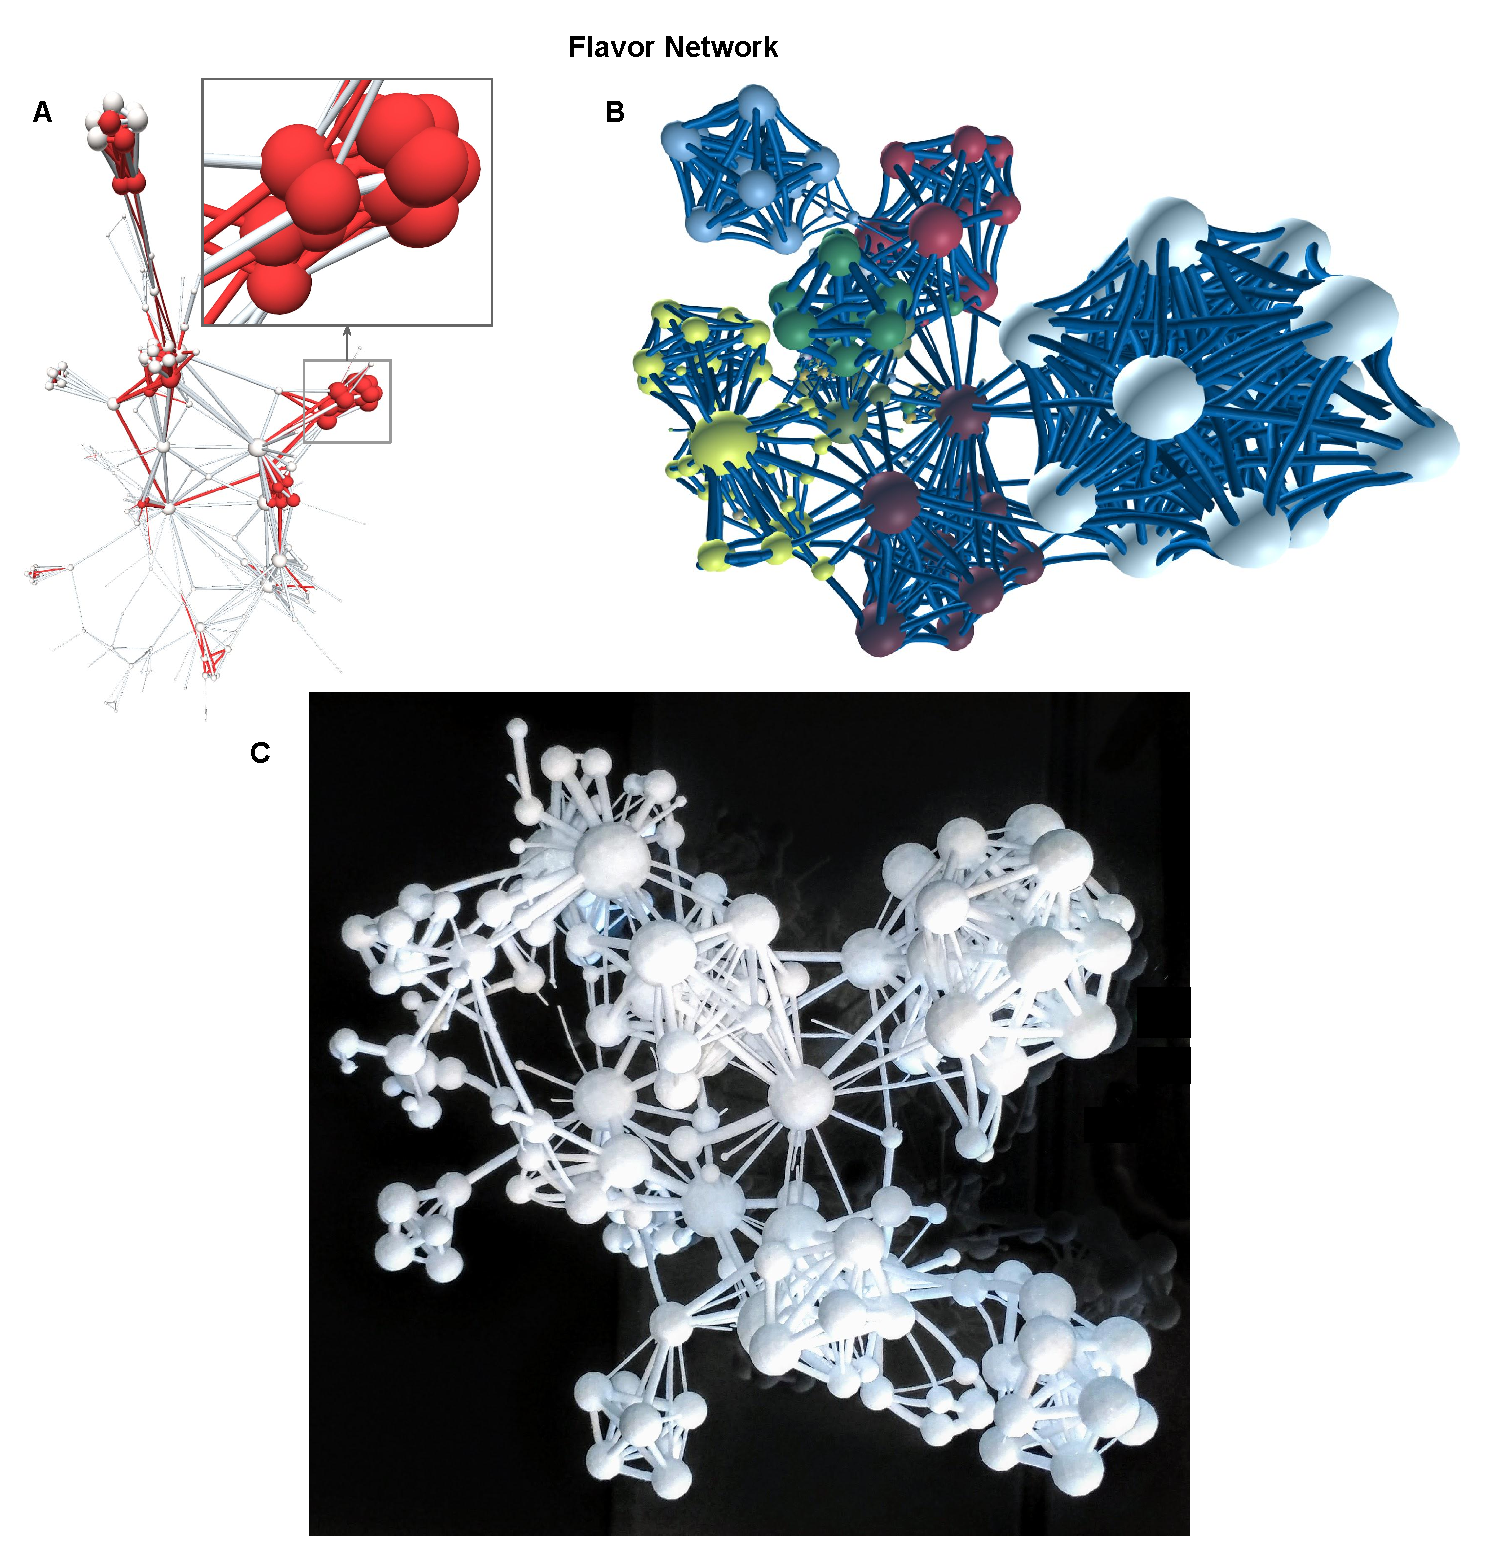
\includegraphics[width=\columnwidth, trim= 0 0 0 1cm, clip]{fig-09-19/3d-flavor-panel.pdf}%{fig-09-19/flavor-3d-print.jpg}
    % 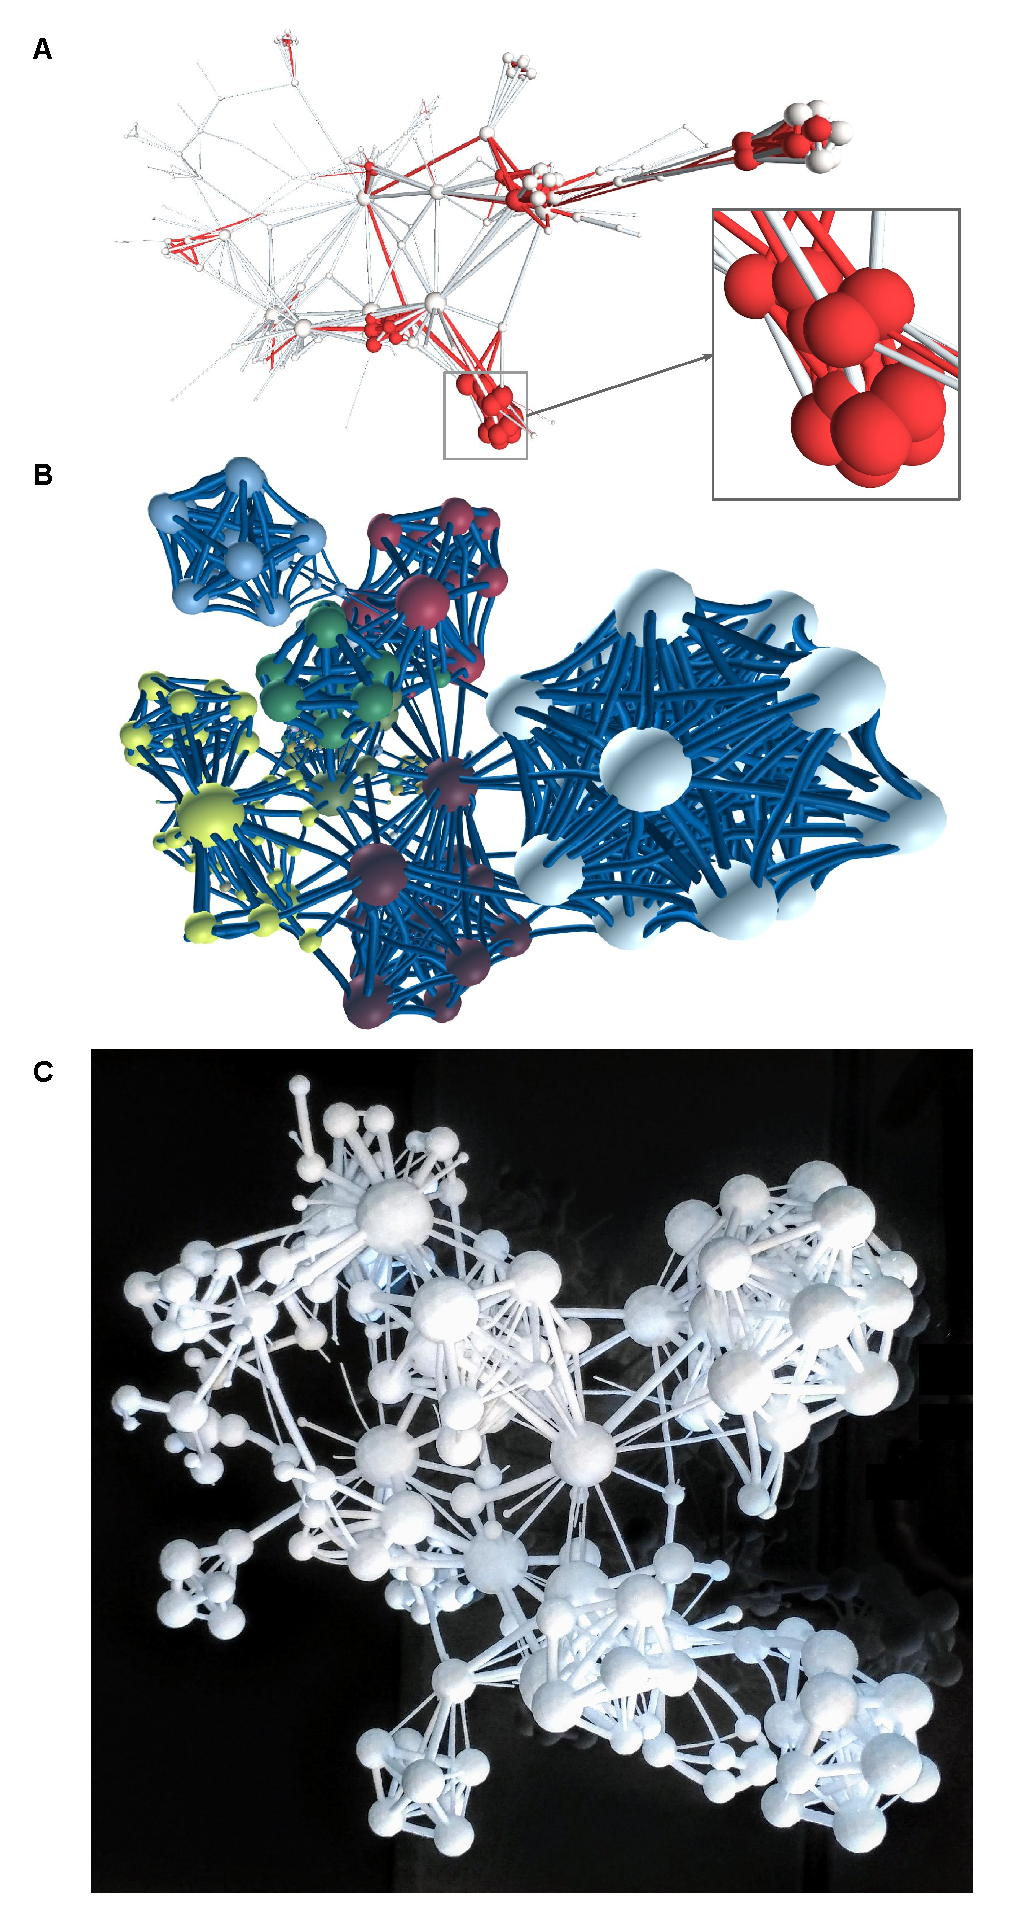
\includegraphics[width=.65\columnwidth ,trim= 0 0 0 1cm%,clip
    % ]{fig-09-19/3D-flavor-panel-092617.pdf}
    % 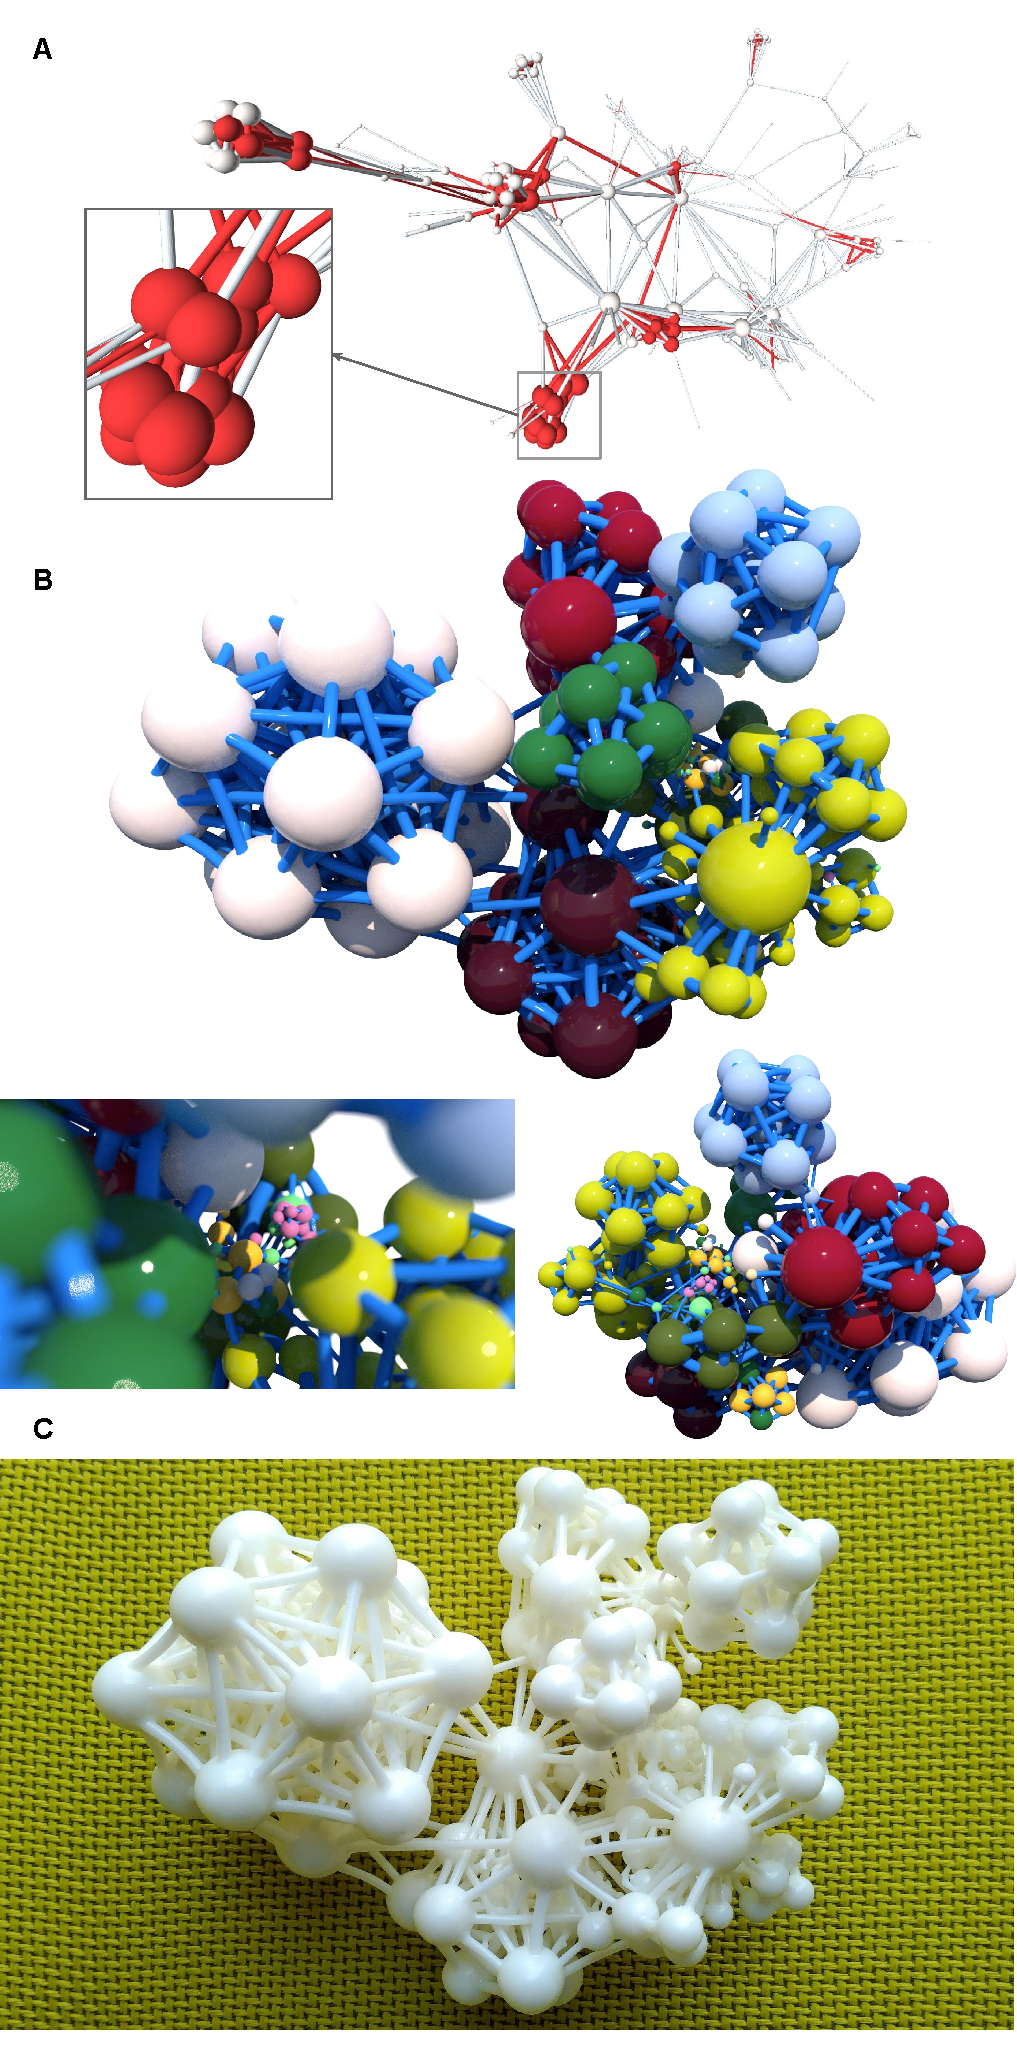
\includegraphics[height=\textheight
    % ]{fig-09-19/3D-flavor-panel-110217.pdf}
    %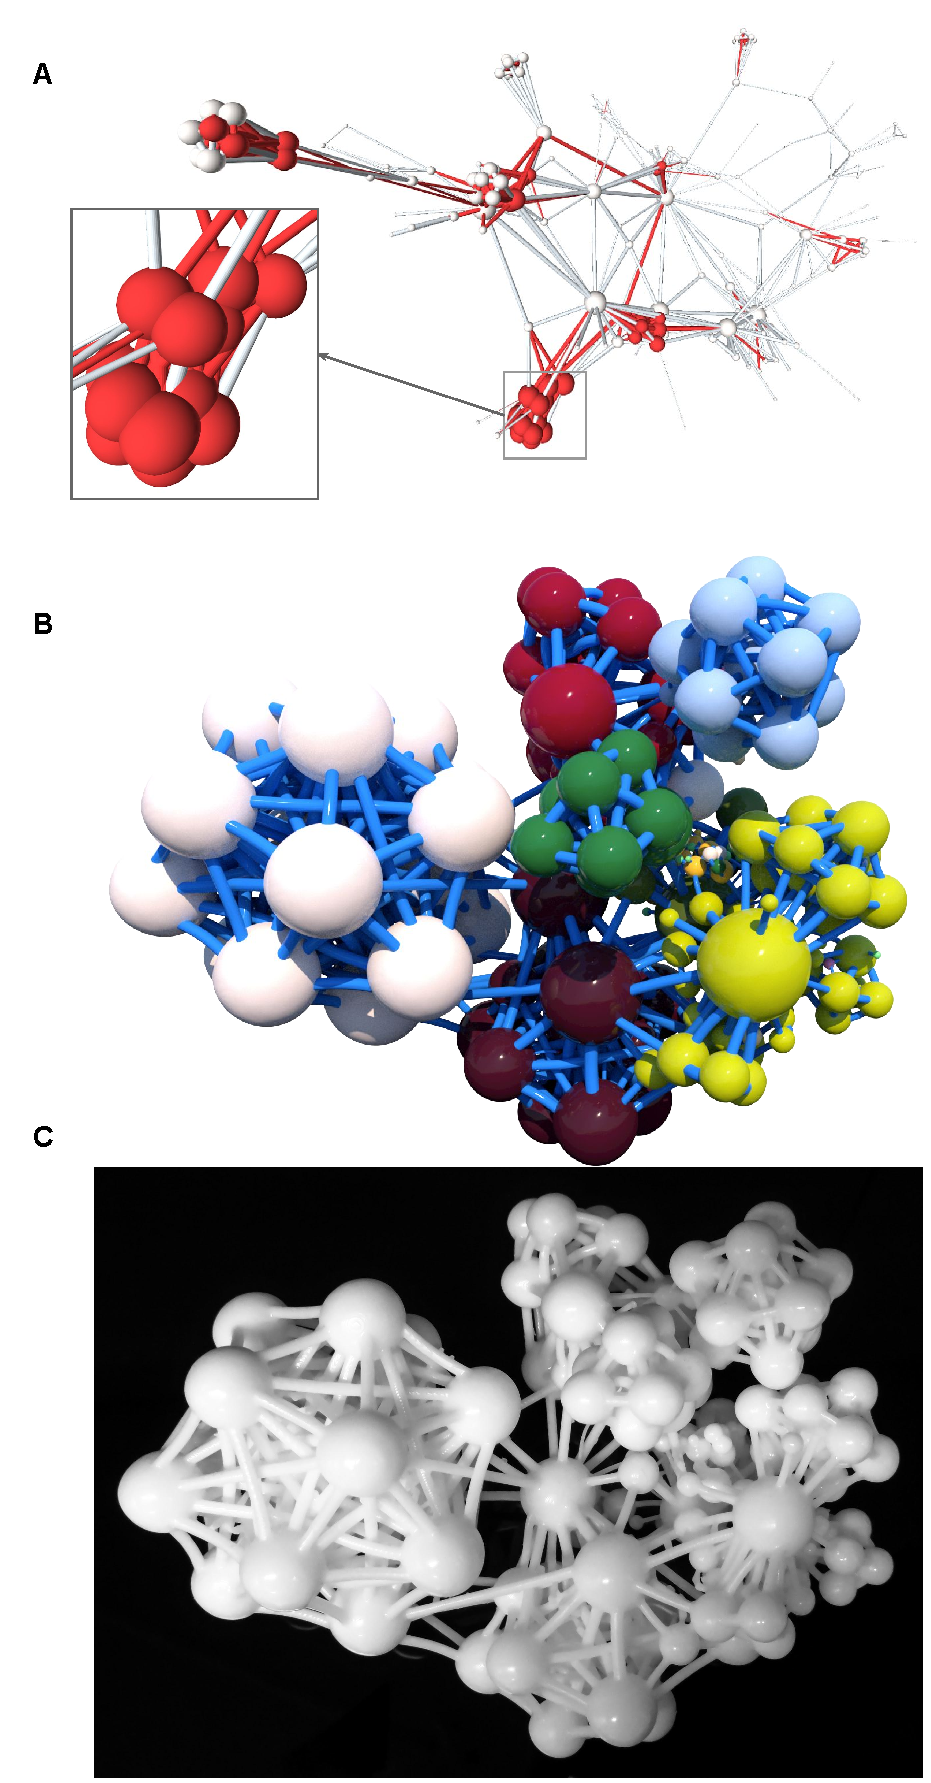
\includegraphics[height=\textheight]{fig-09-19/3D-flavor-panel-110317.pdf}
    %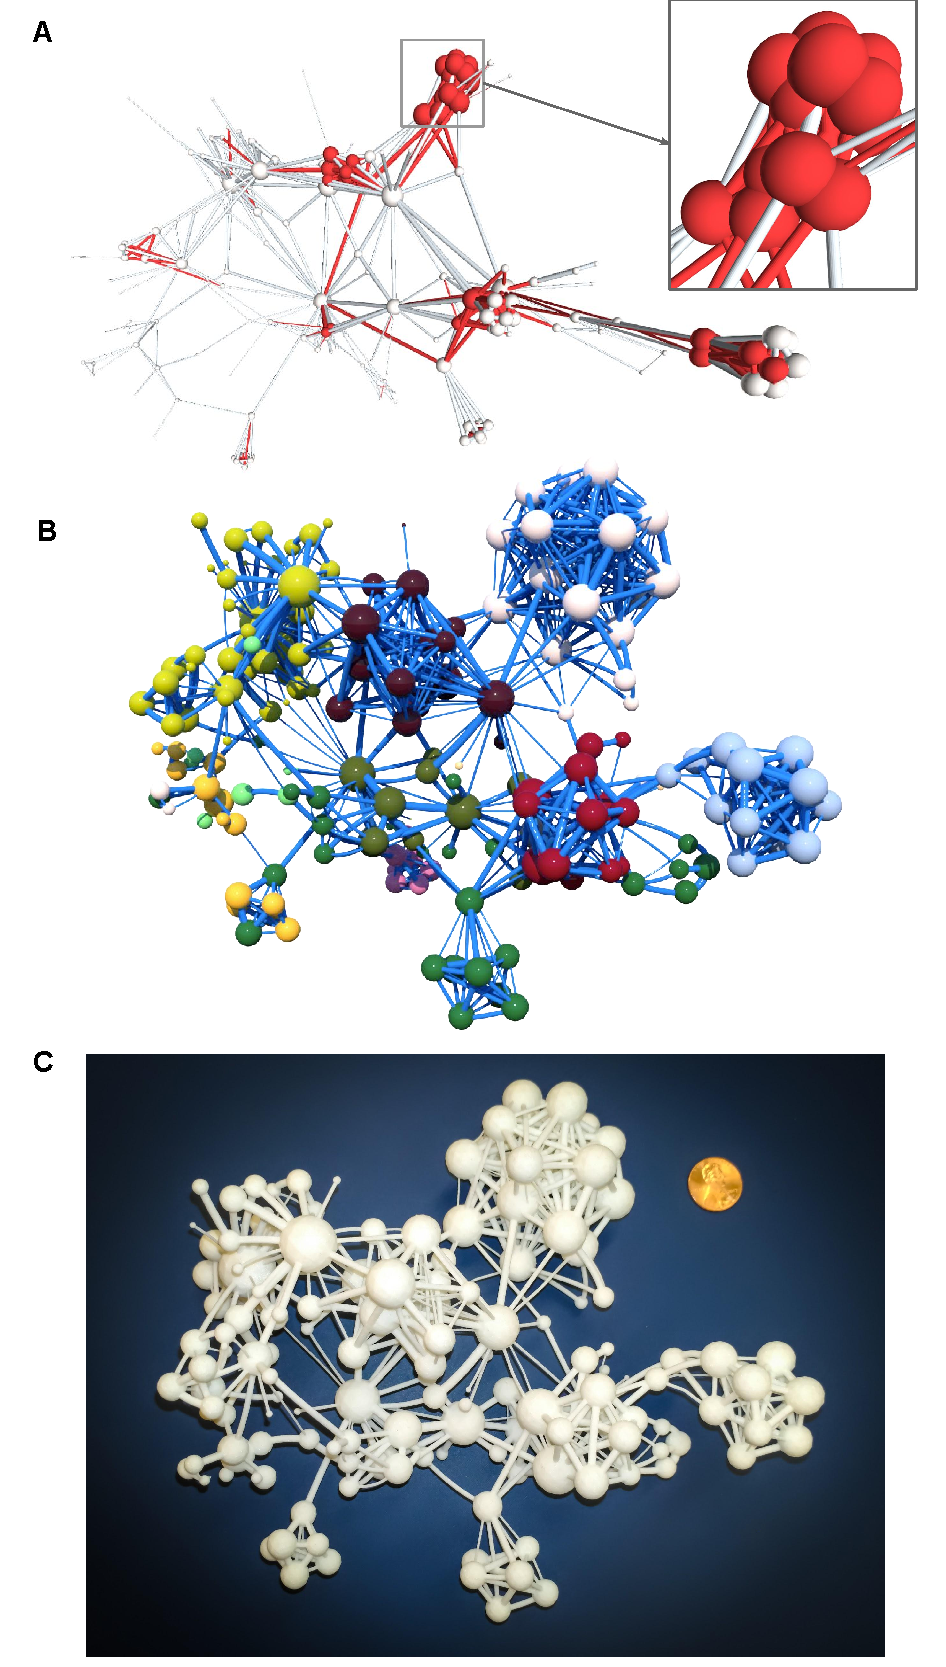
\includegraphics[height=\textheight]{fig-09-19/Flavor-111217.pdf}
    %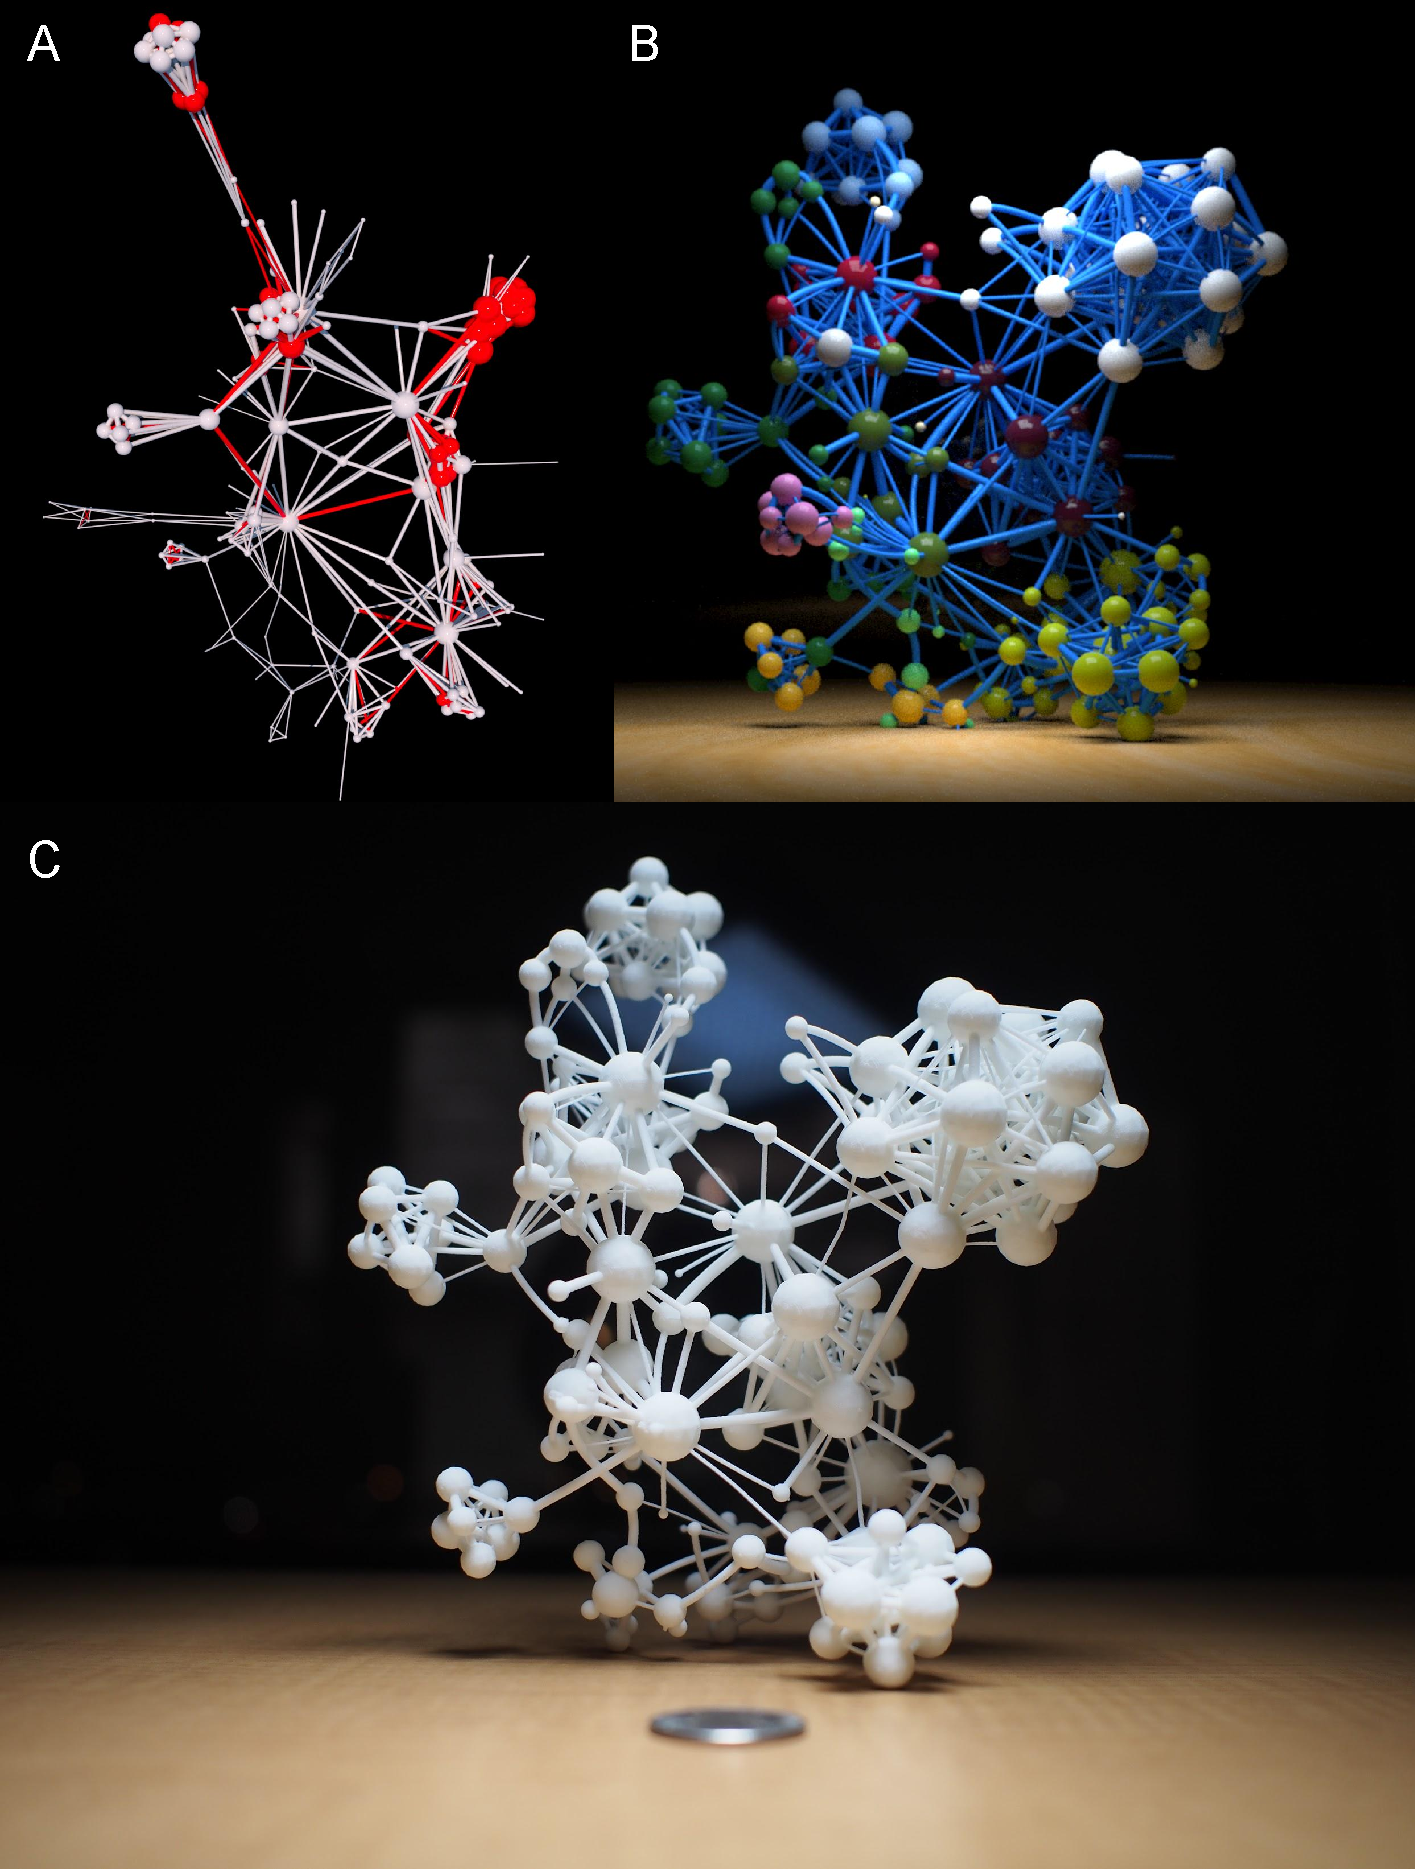
\includegraphics[height=\textheight]{fig-09-19/3D-flavor-111917-1.pdf}
    %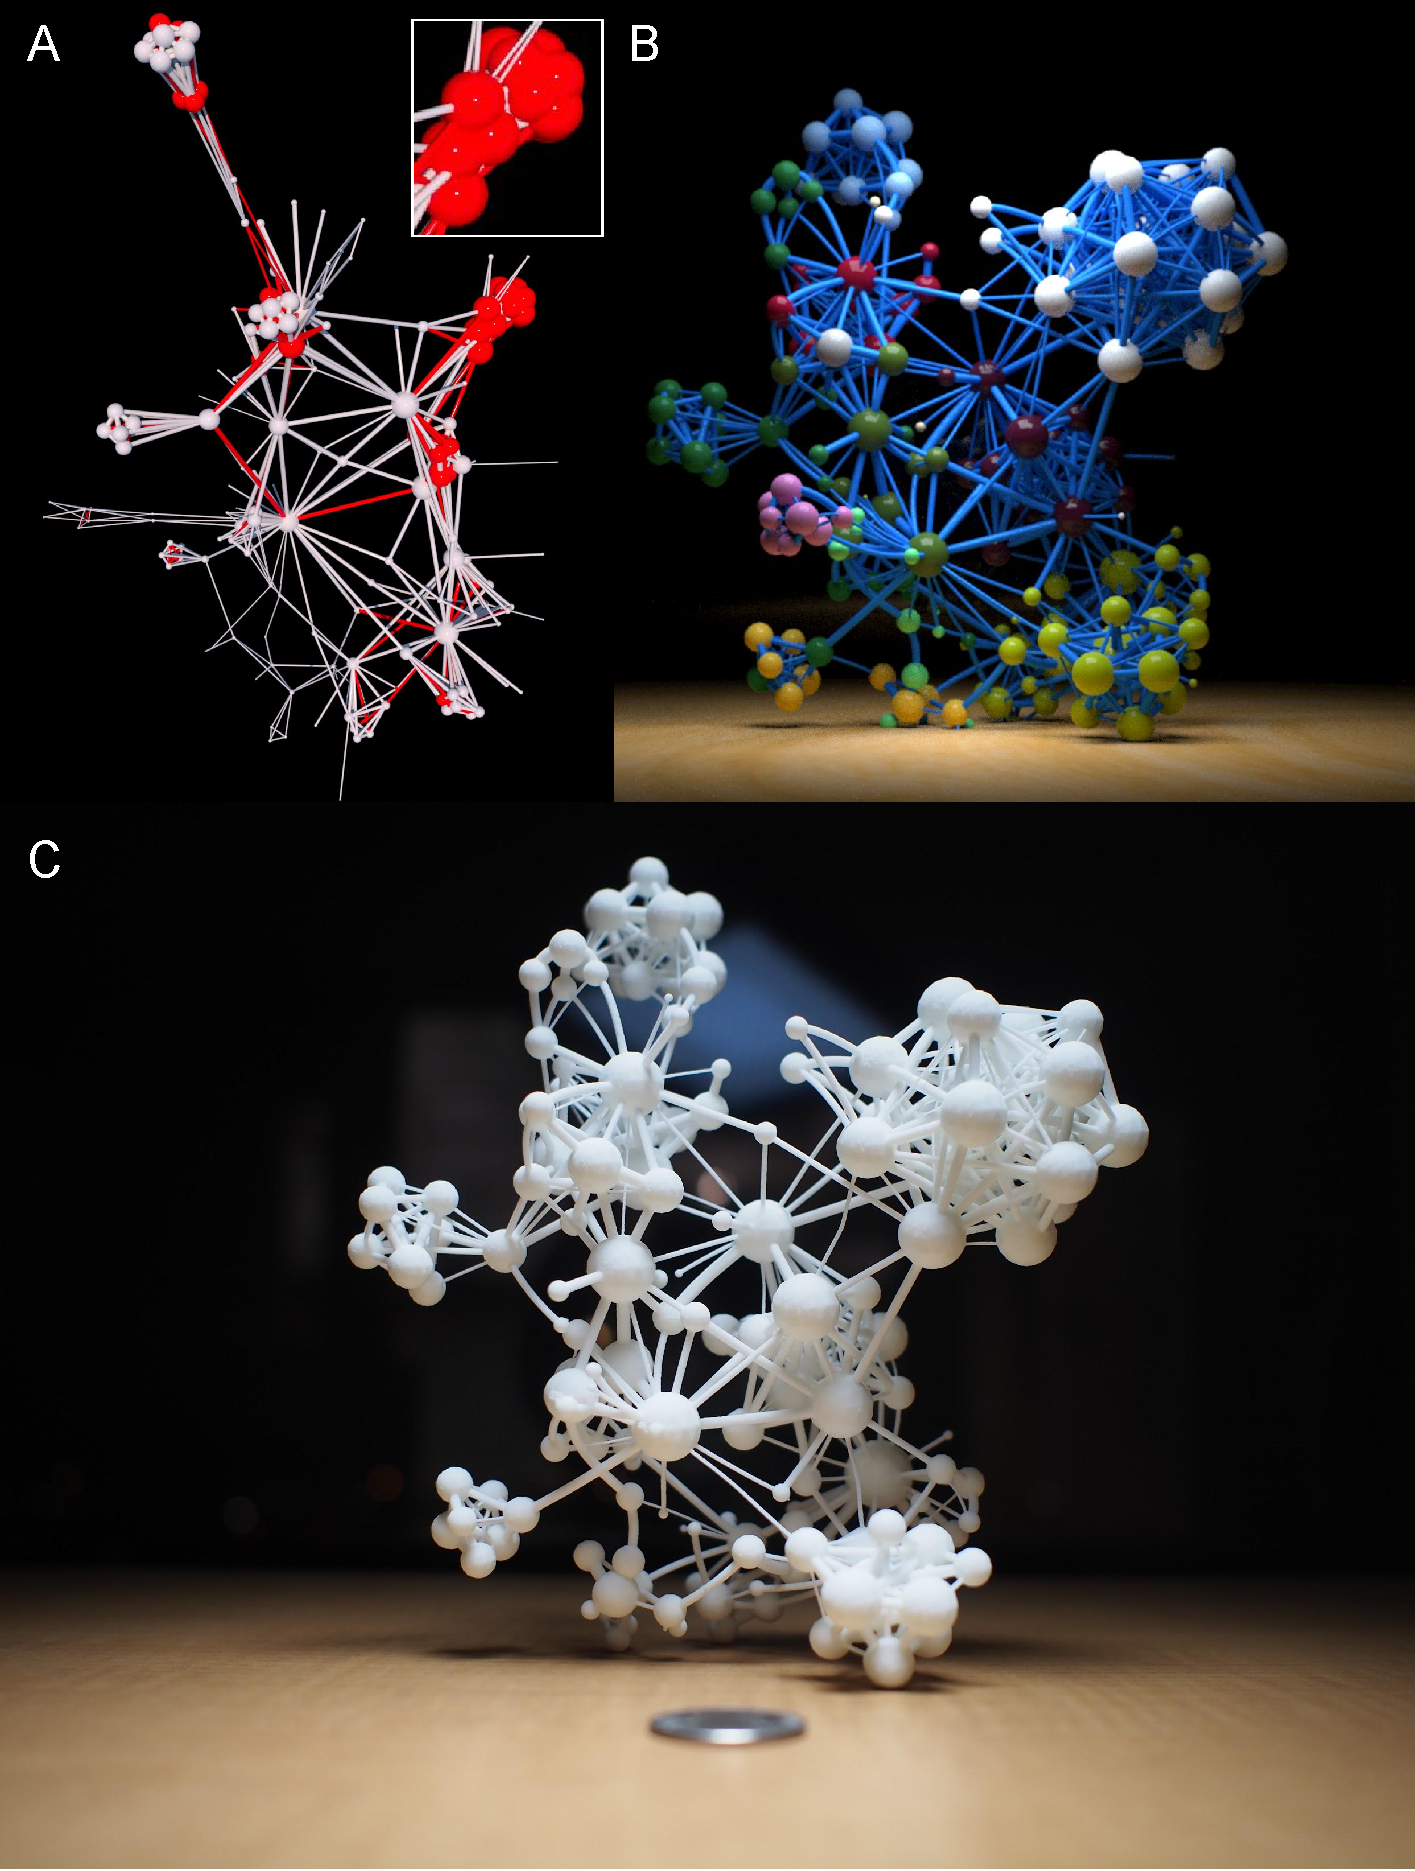
\includegraphics[height=\textheight]{fig-09-19/3D-flavor-111917-1-2.pdf}
    %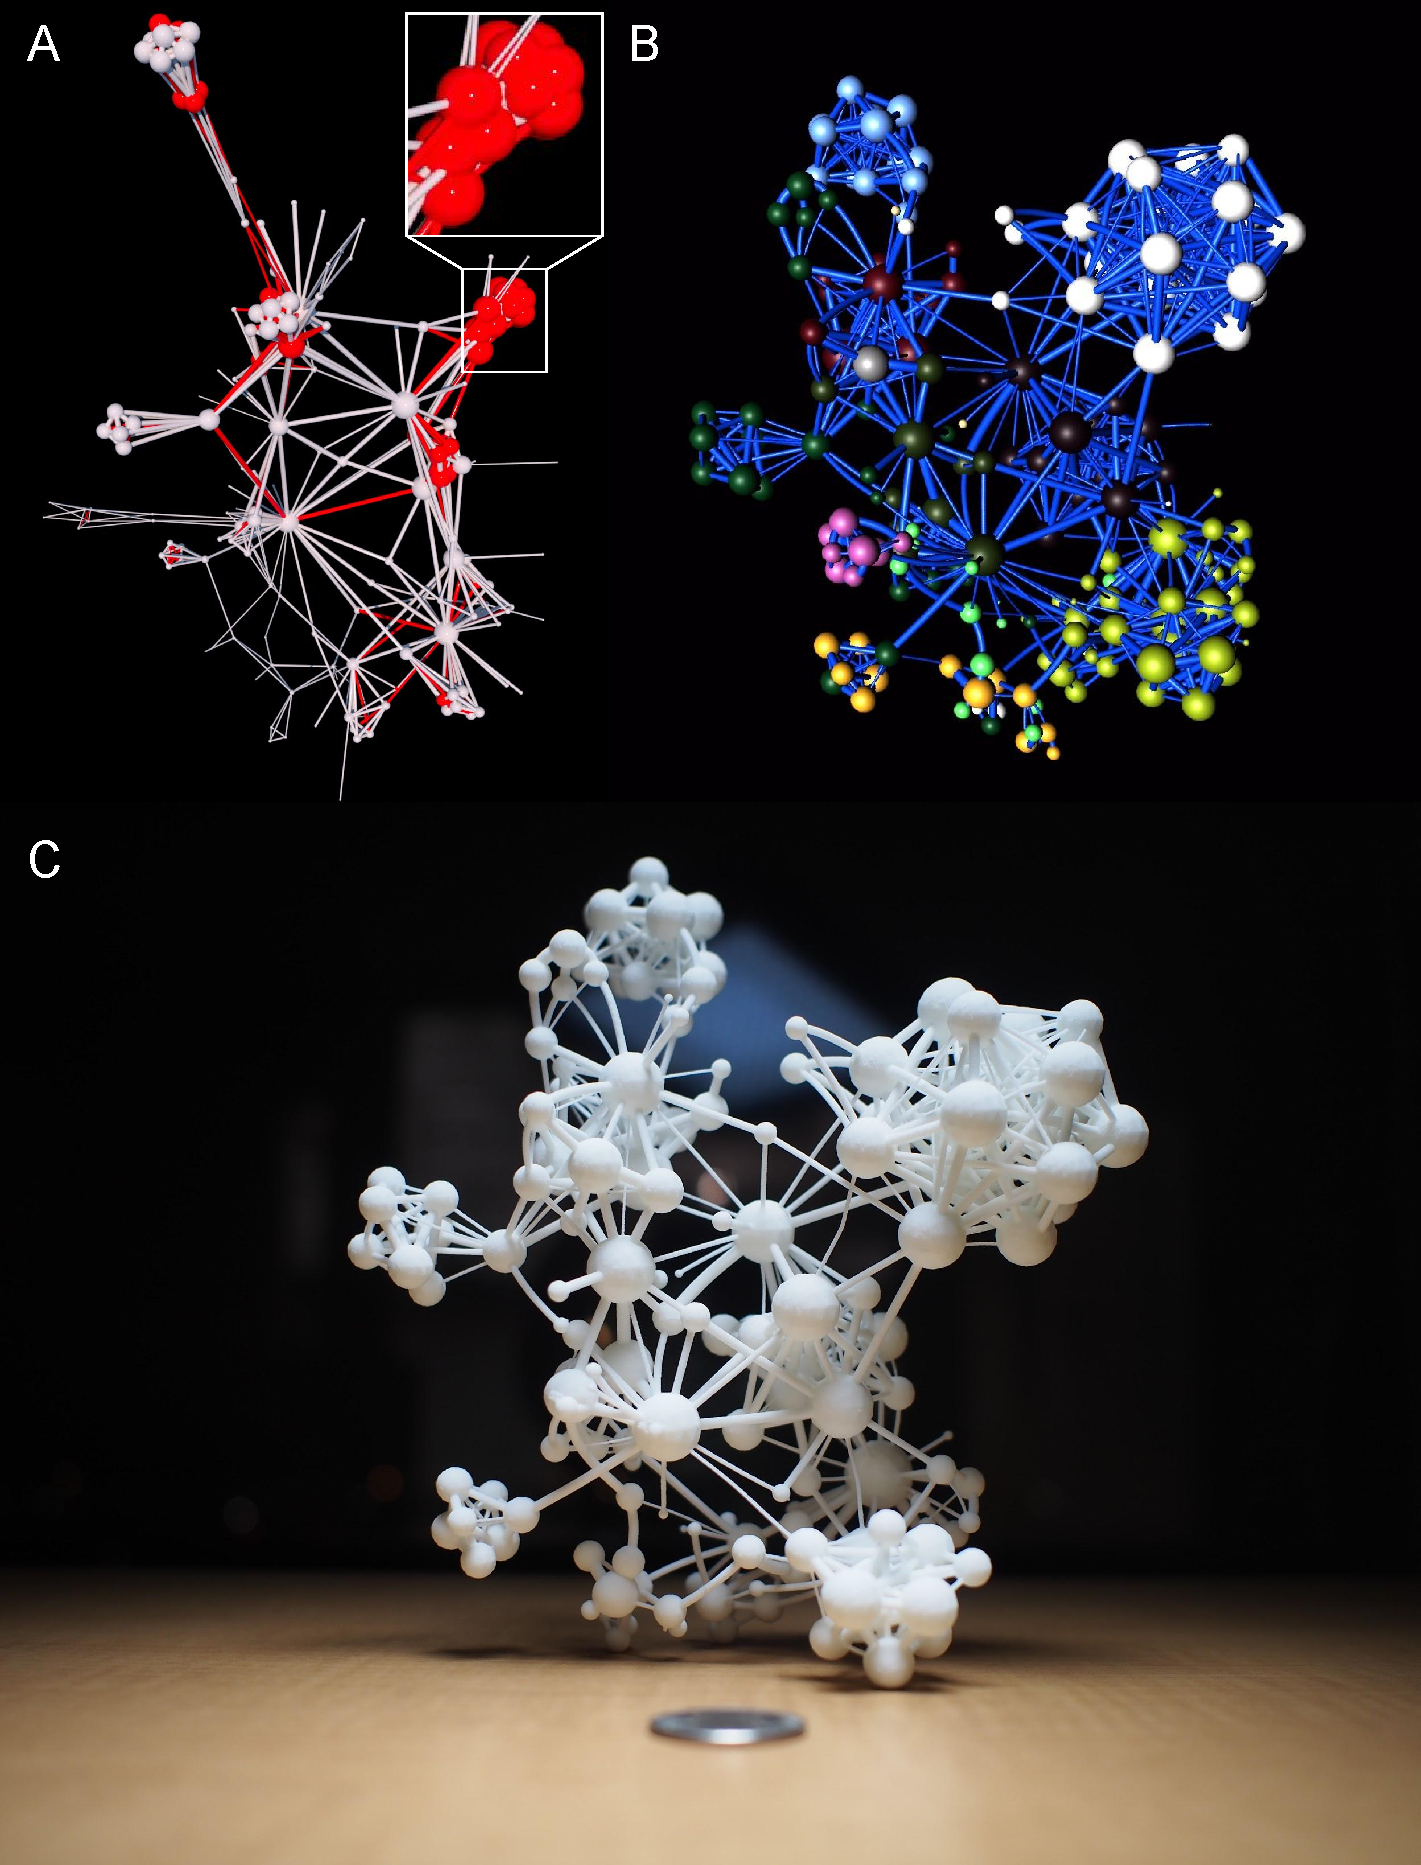
\includegraphics[height=\textheight]{fig-09-19/3D-flavor-111917-1-3.pdf}
    % 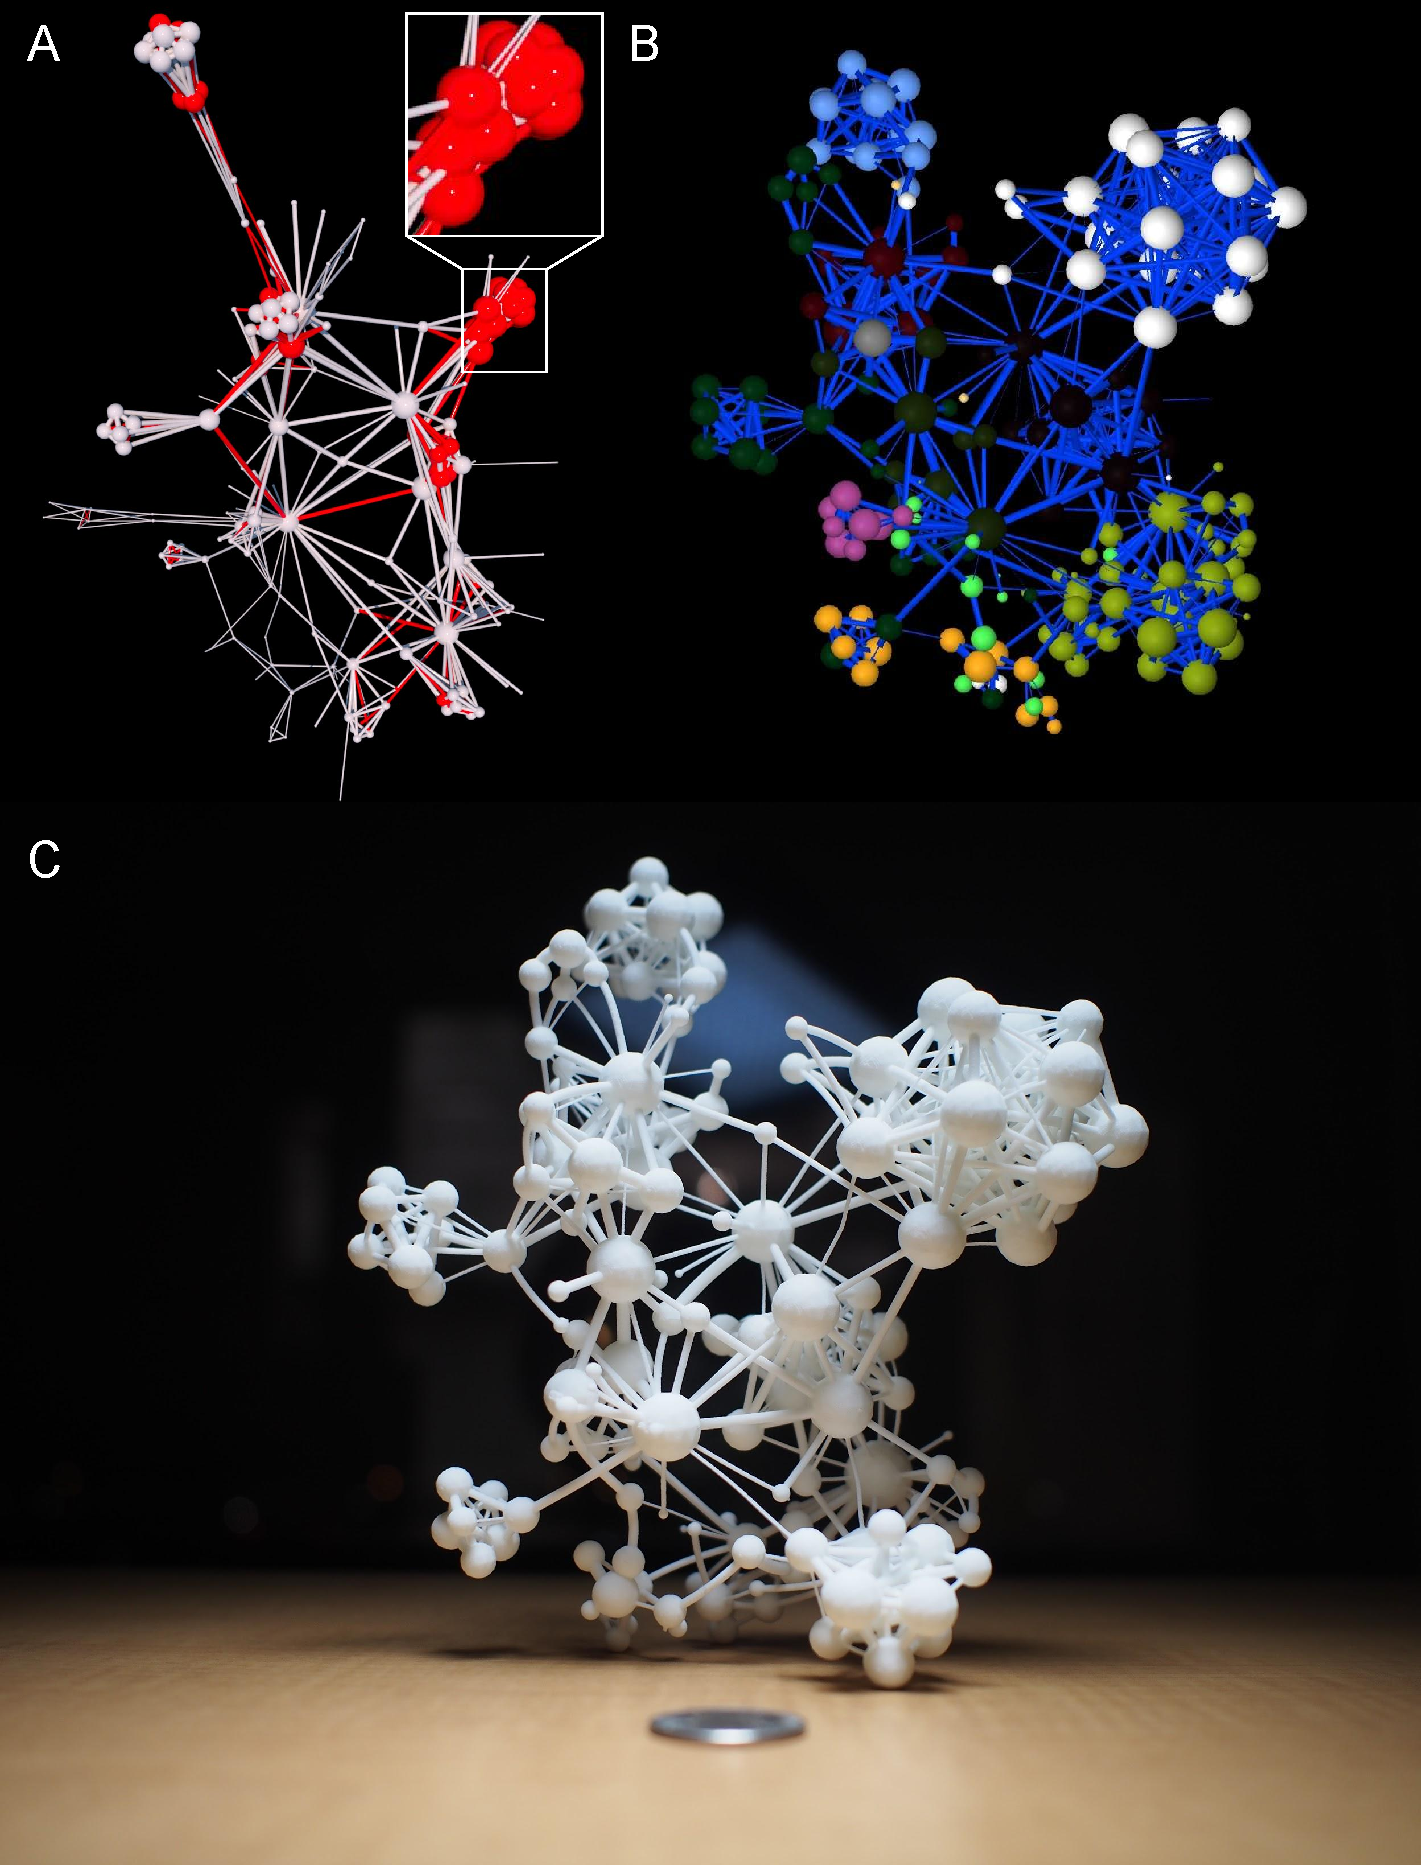
\includegraphics[height=\textheight]{fig-09-19/3D-flavor-111917-1-4.pdf}
    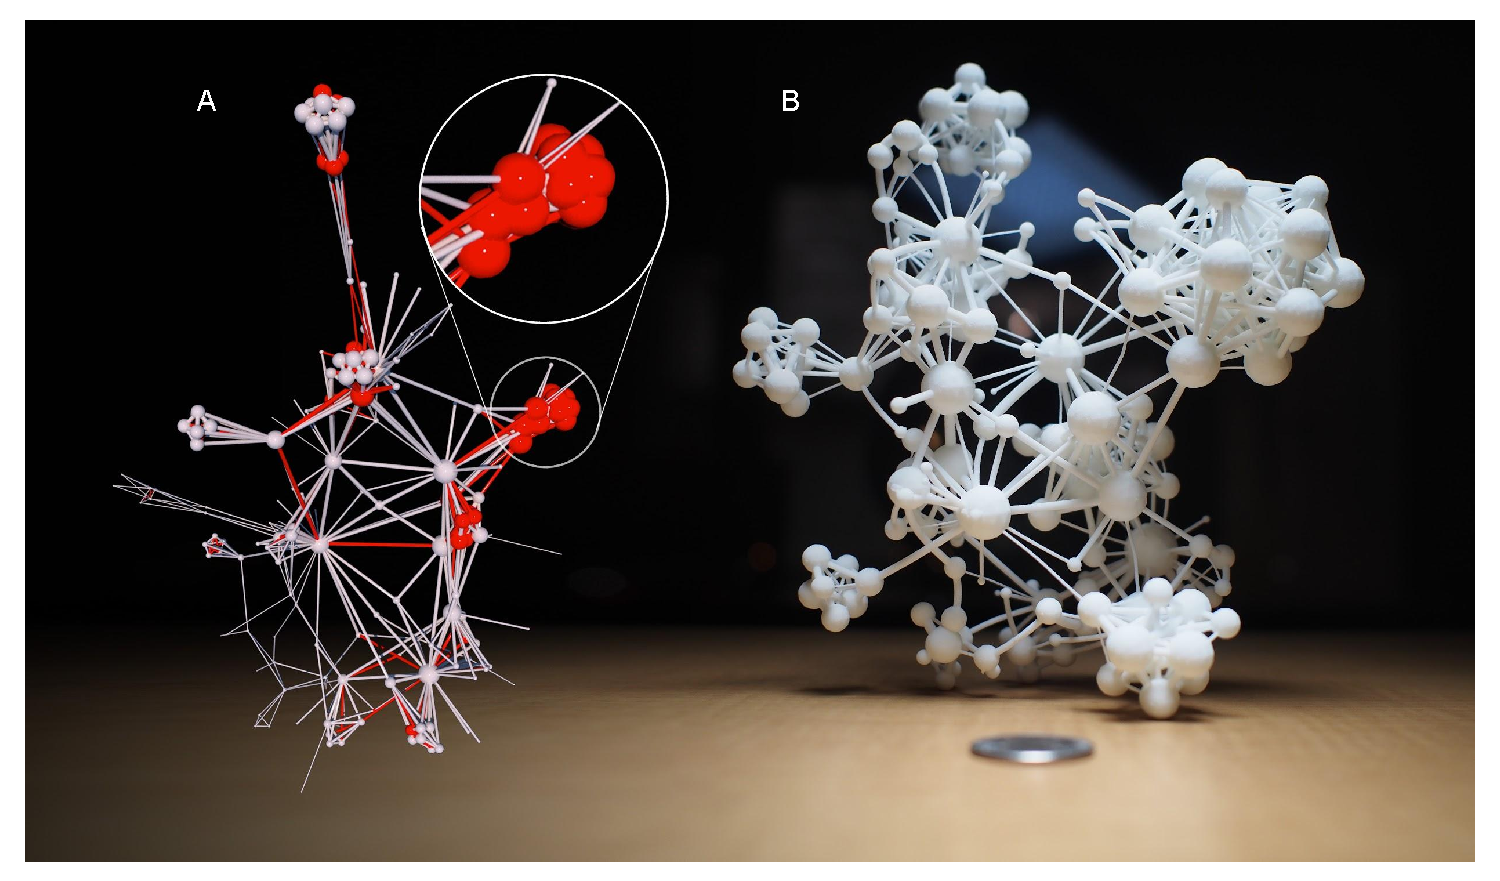
\includegraphics[width=\textwidth]{fig-09-19/3D-flavor-112117-1.pdf}
    \caption{\scriptsize {\bf 3D Printing of Networks:}
    The Flavor Network with $N=184$, $L=716$, represents a network of ingredients connected by links whose weights capture the number of times two ingredients appear together in recipes. 
    %In 2D only a pruned network could be shown before \cite{ahn2011flavor}, given the high link density.
    A 3D layout avoids this problem. 
    {\bf (A)} An FDL layout applied to this network results in multiple conflicts.
    Nodes and links with conflicts are highlighted in red. 
    The inset highlights a densely connected region containing nodes for dairy products,
    so highly overlapping that it is impossible to discern the underlying network relationships.
    %characterized by an exceptional number of local conflicts. 
    %Even with very thin links, simple FDL exhibits many conflicts. 
    {\bf (B)} If we lay out the flavor network using FUEL, the conflicts disappear, 
    unveiling the inner structure of the communities \cite{fortunato2010community}
    present in the network. 
    % For clarity nodes are colored based on the food category they belong to. 
    % The white nodes correspond to dairy, indicating that 
    % FUEL has %both efficiently assigned enough room for nodes and has 
    % resolved the earlier conflicts, pulling apart the highly connected region of the dairy module.  
    %{\bf (C)} 
    We 3D printed the resulting flavor network using a commercial 3D printer, allowing us to inspect the full internal structure of the network. %  \cite{ahn2011flavor}. 
    The varying node sizes are proportional to the total strengths of the node connections % (root sum squared of its link weights, 
    (\ref{ap:params}). 
    % Only diseases with $s_{AB} $ more than 2 sigma below the average $s_{AB}$ have been considered. 
    % The link thickness is based on $|s_{AB}|$. 
    }
    \label{fig:3d-print}
    \newpage
\end{figure}
\outNim{
\begin{figure}
    \centering
    %\vspace{-2cm}
    %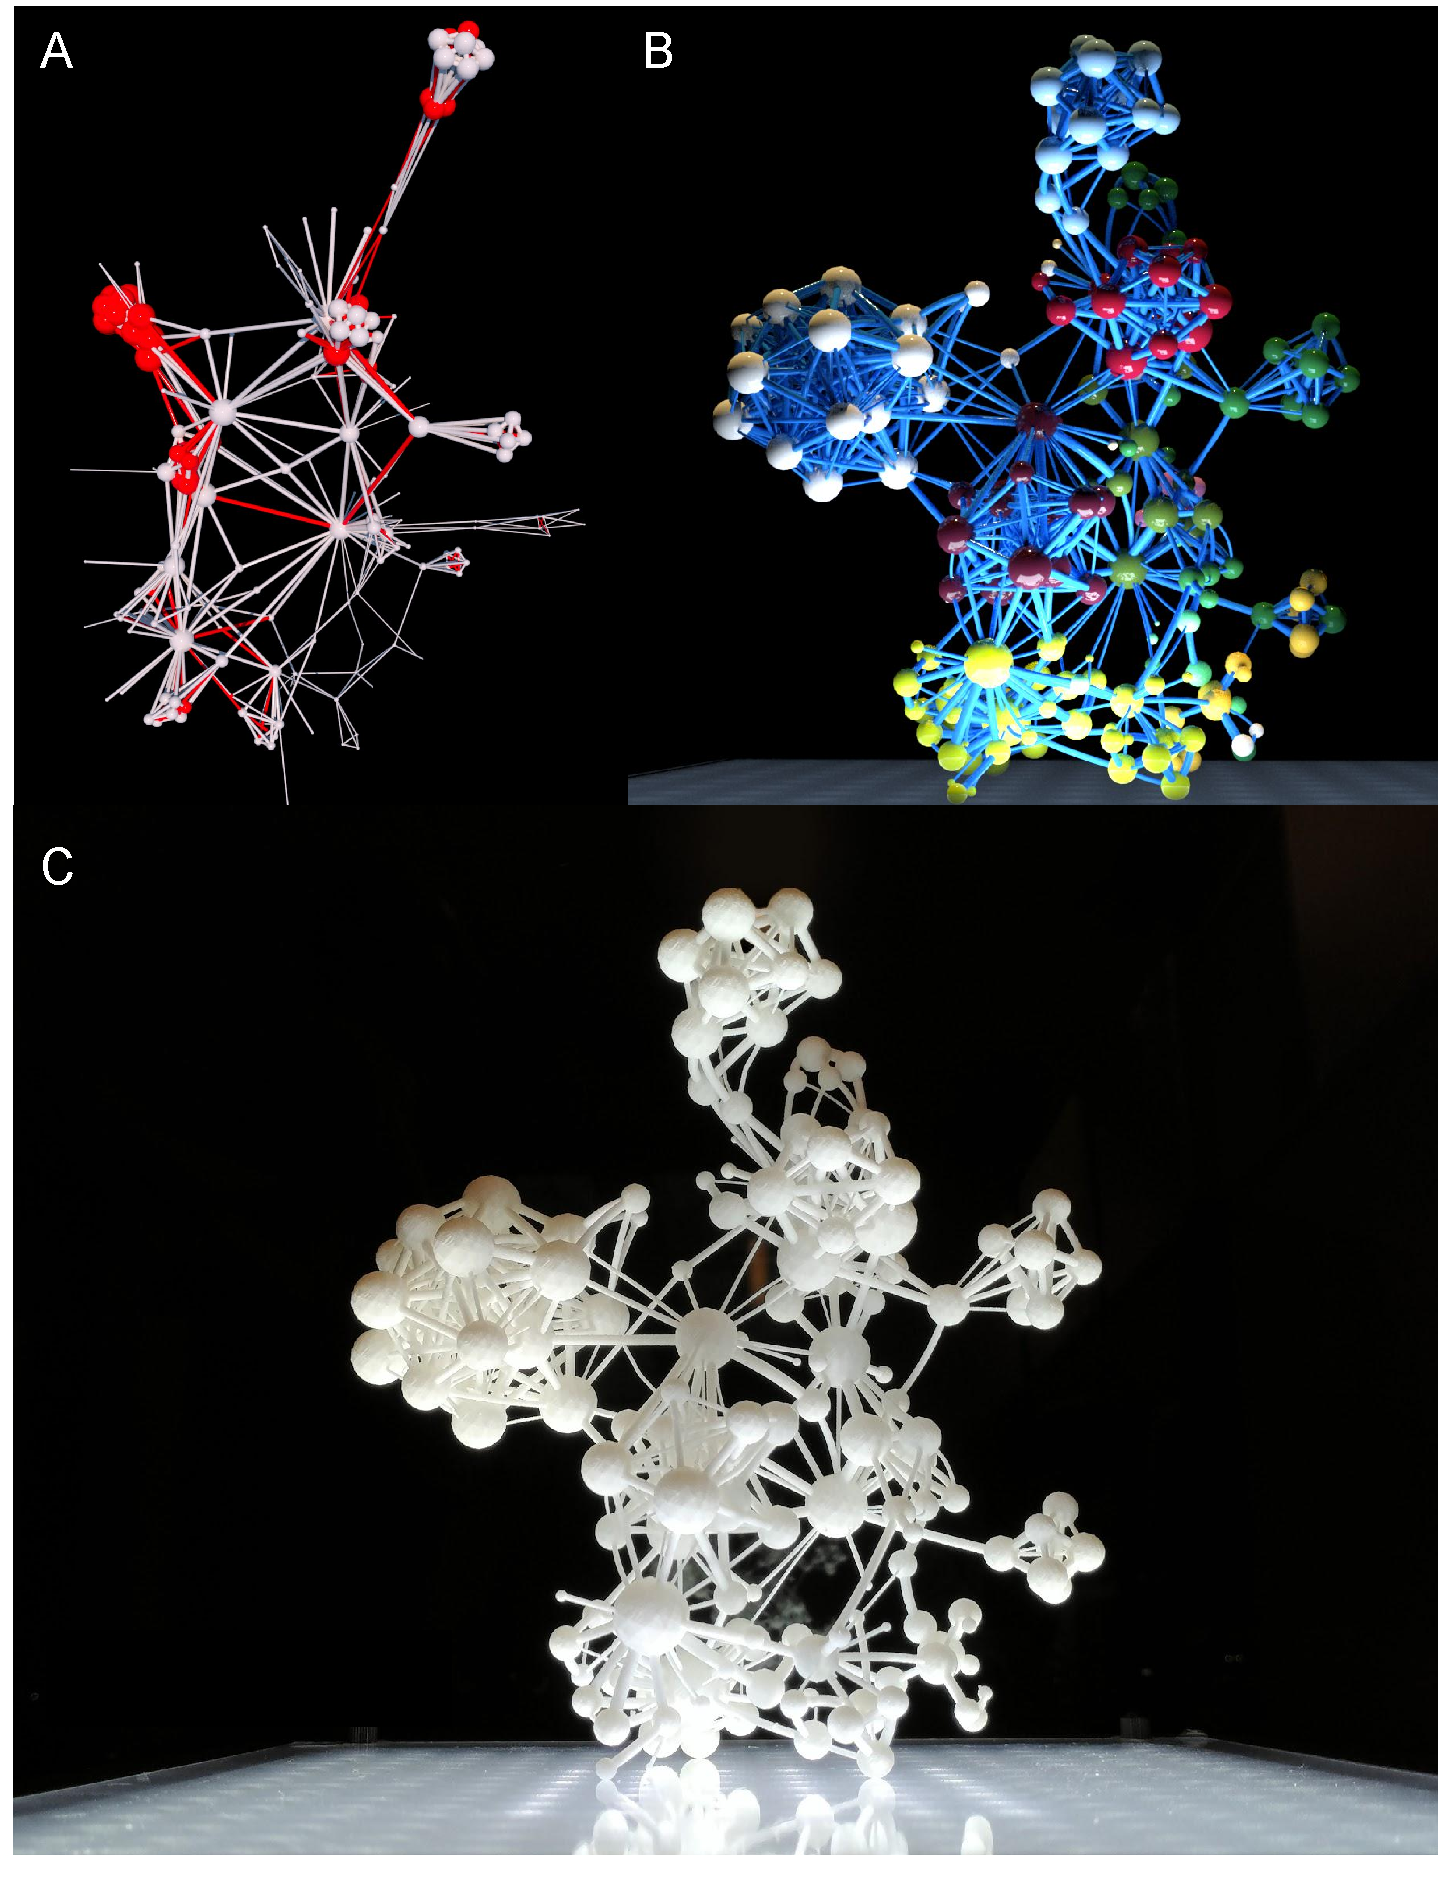
\includegraphics[height=\textheight]{fig-09-19/3D-flavor-111917-2.pdf}
    %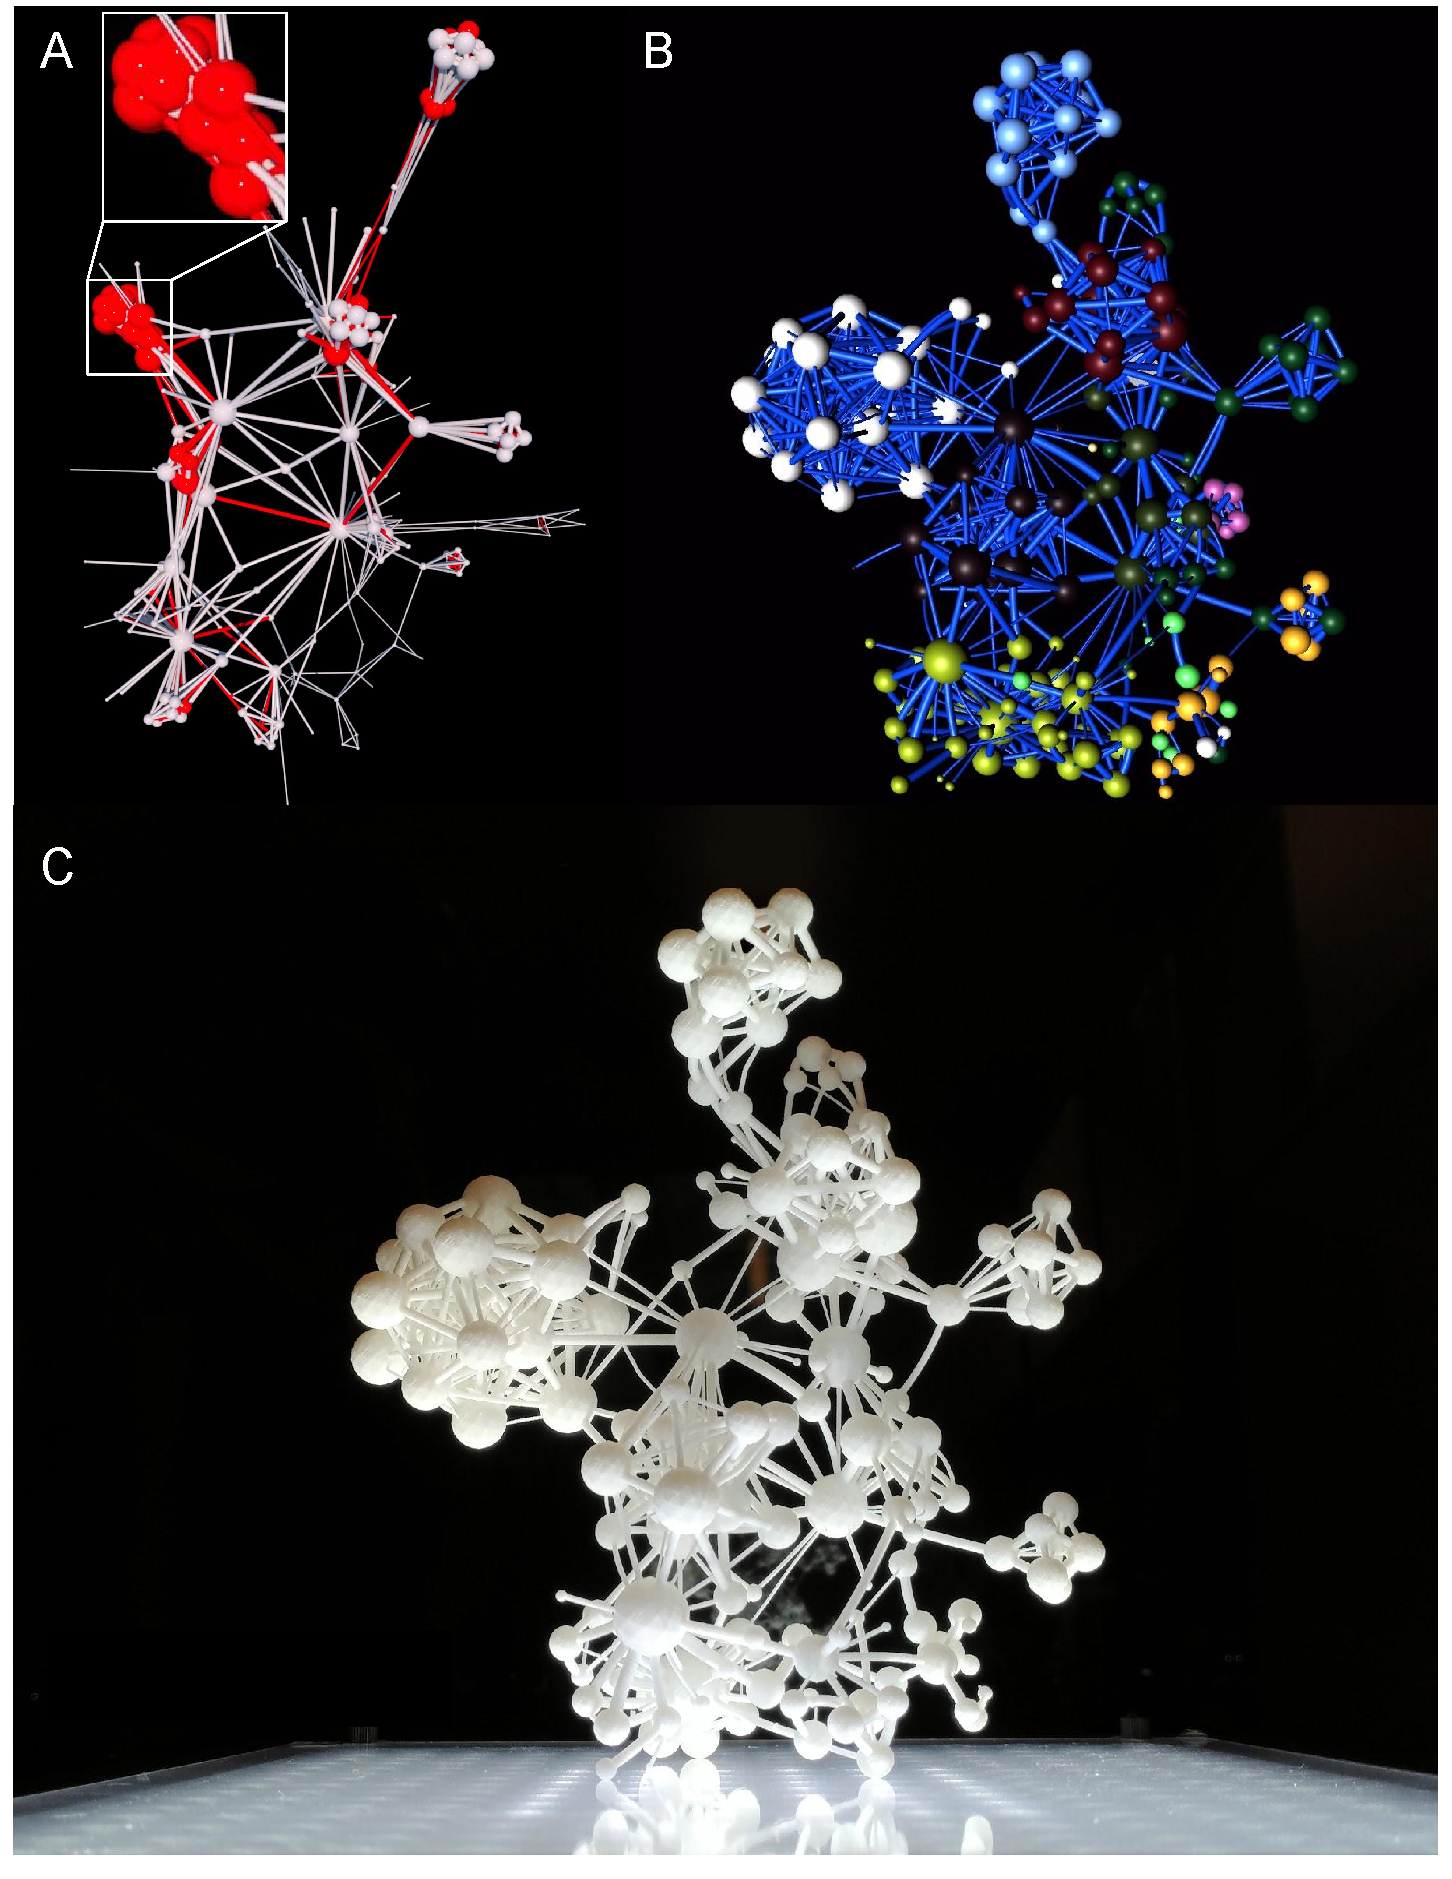
\includegraphics[height=\textheight]{fig-09-19/3D-flavor-111917-2-1.pdf}
    %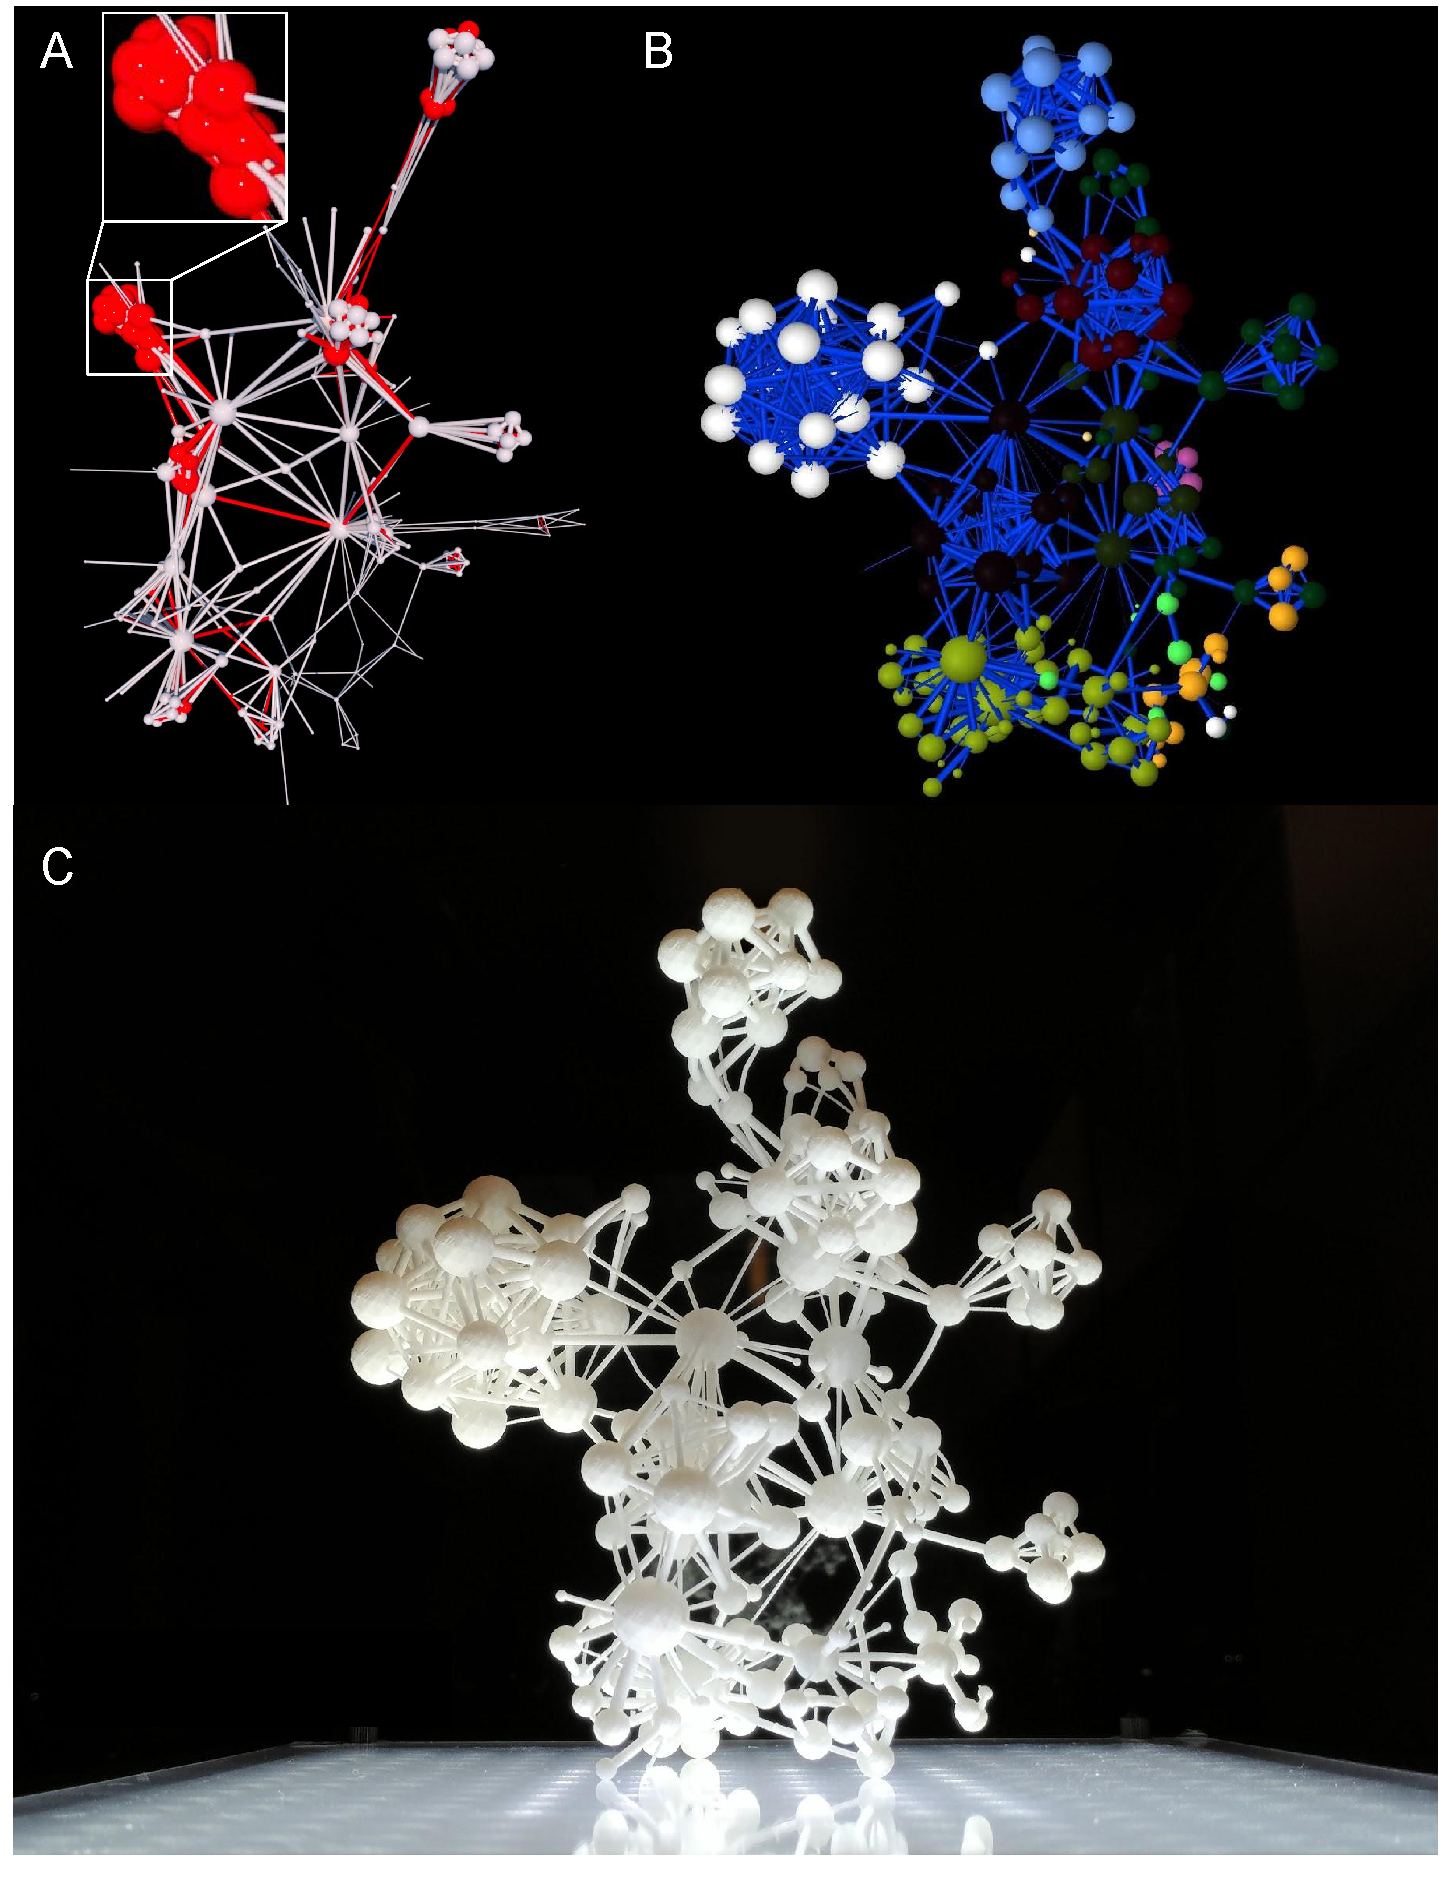
\includegraphics[height=\textheight]{fig-09-19/3D-flavor-111917-2-2.pdf}
    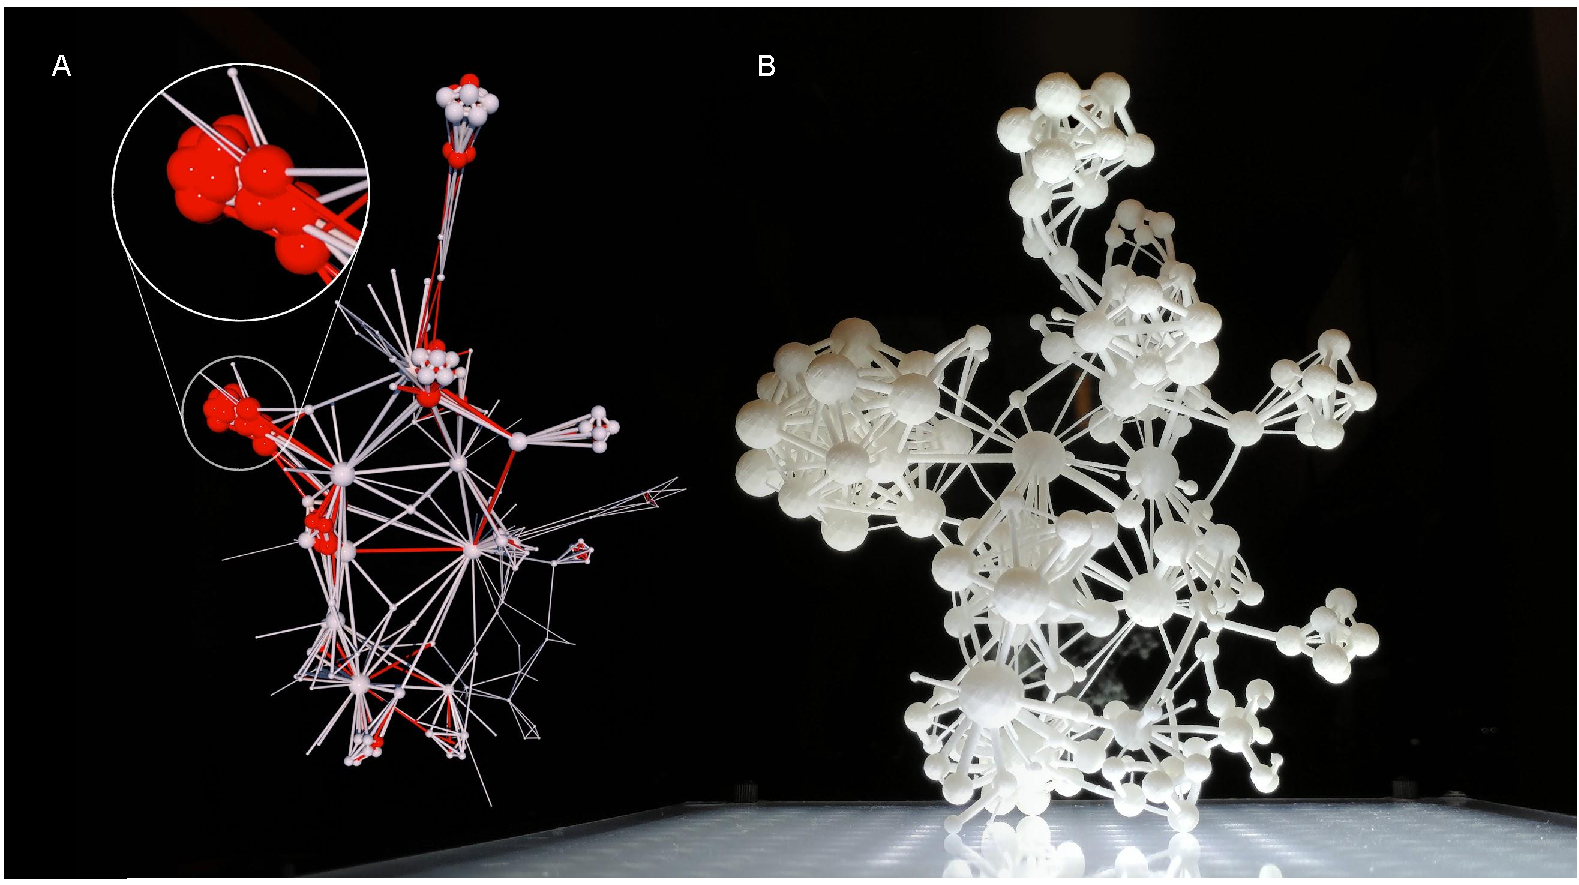
\includegraphics[width=\textwidth]{fig-09-19/3D-flavor-112117-2.pdf}
    \newpage
\end{figure}
\begin{figure}
    \centering
    \vspace{-2cm}
    % 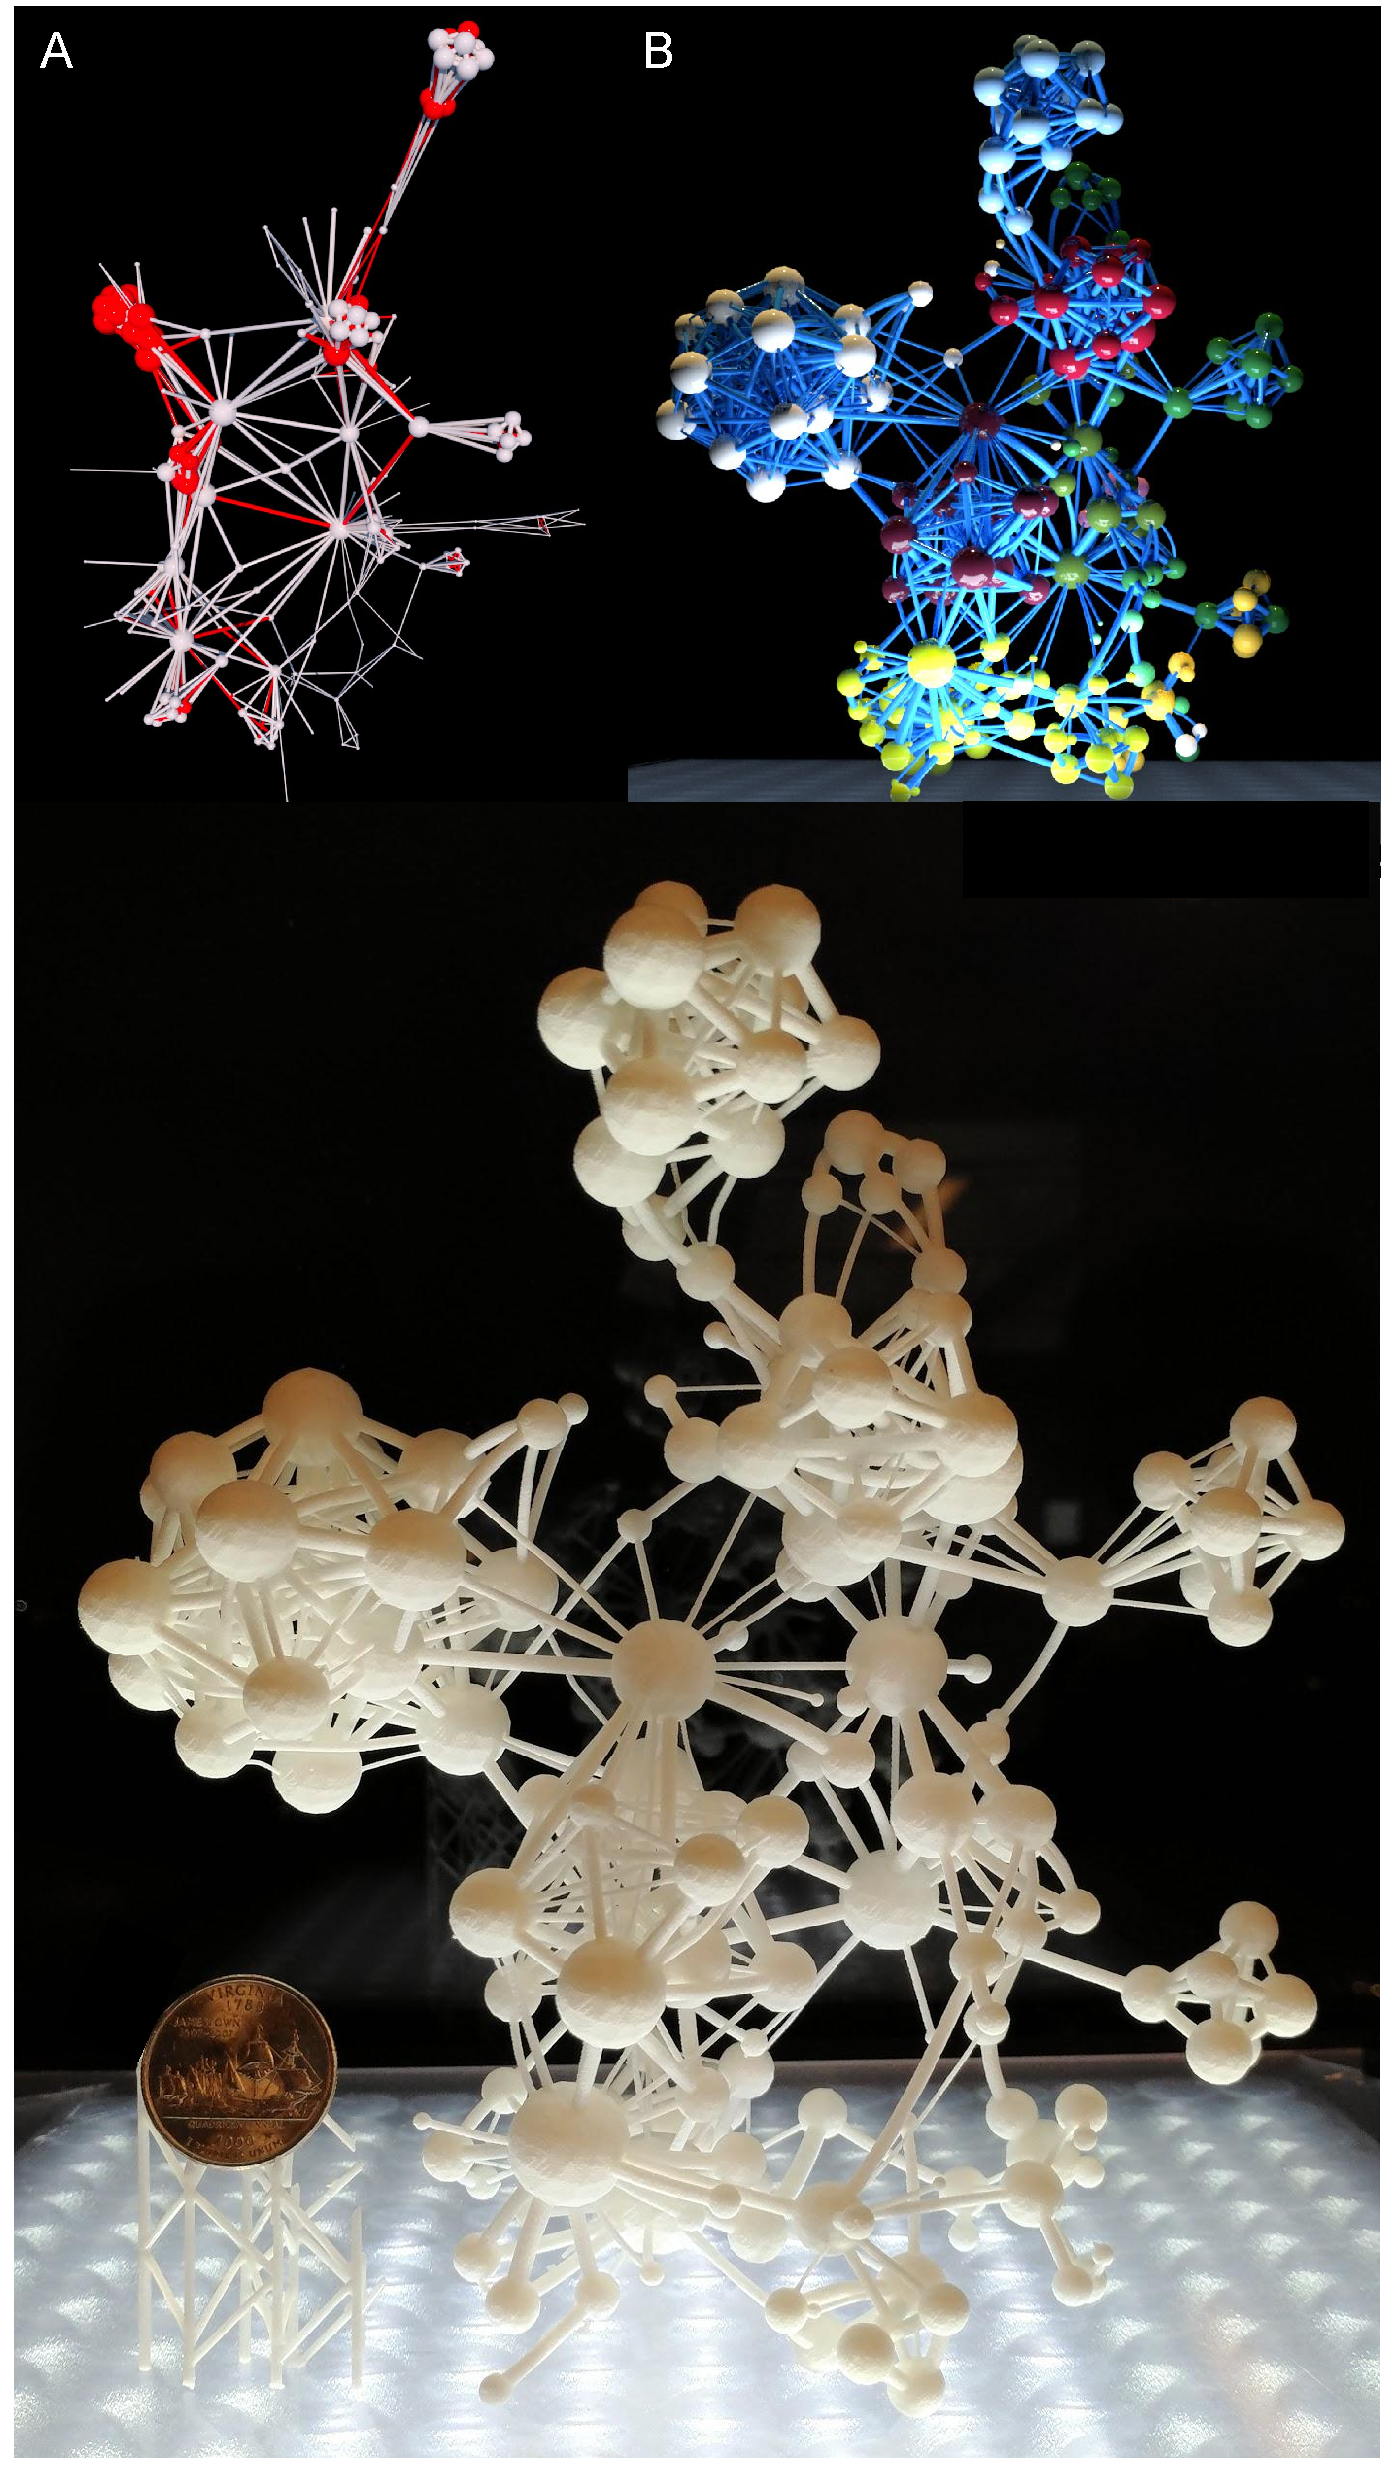
\includegraphics[height=\textheight]{fig-09-19/3D-flavor-111917-3.pdf}
    % 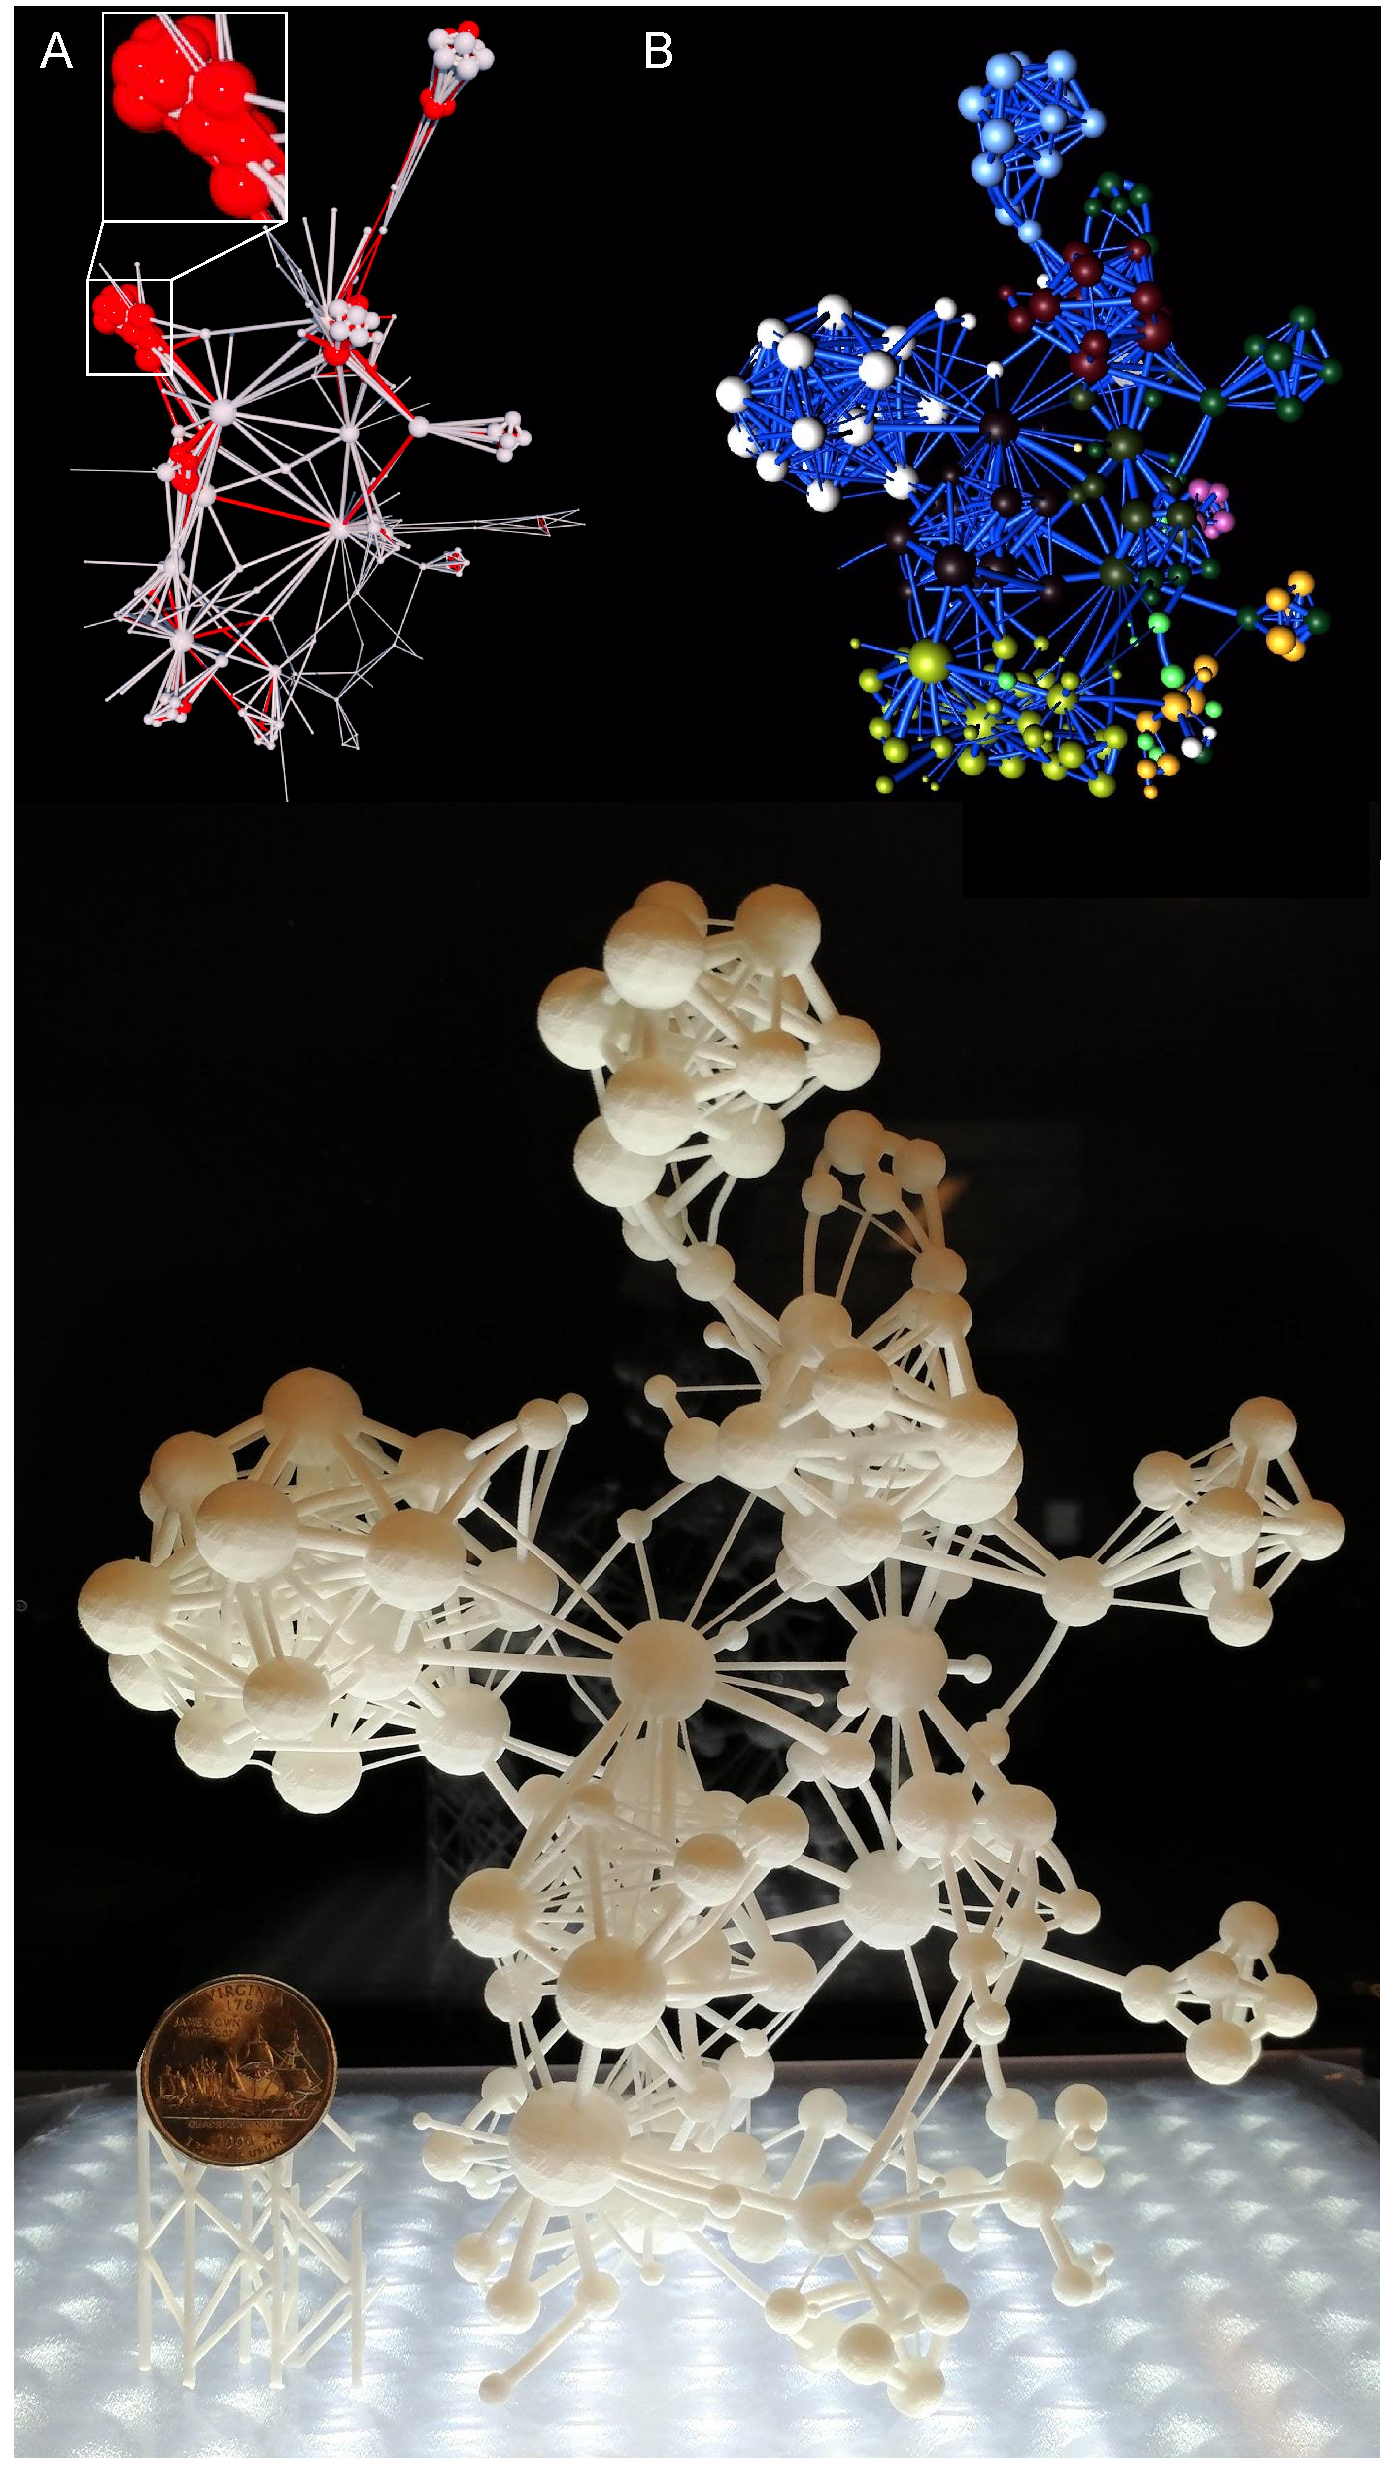
\includegraphics[height=\textheight]{fig-09-19/3D-flavor-111917-3-1.pdf}
    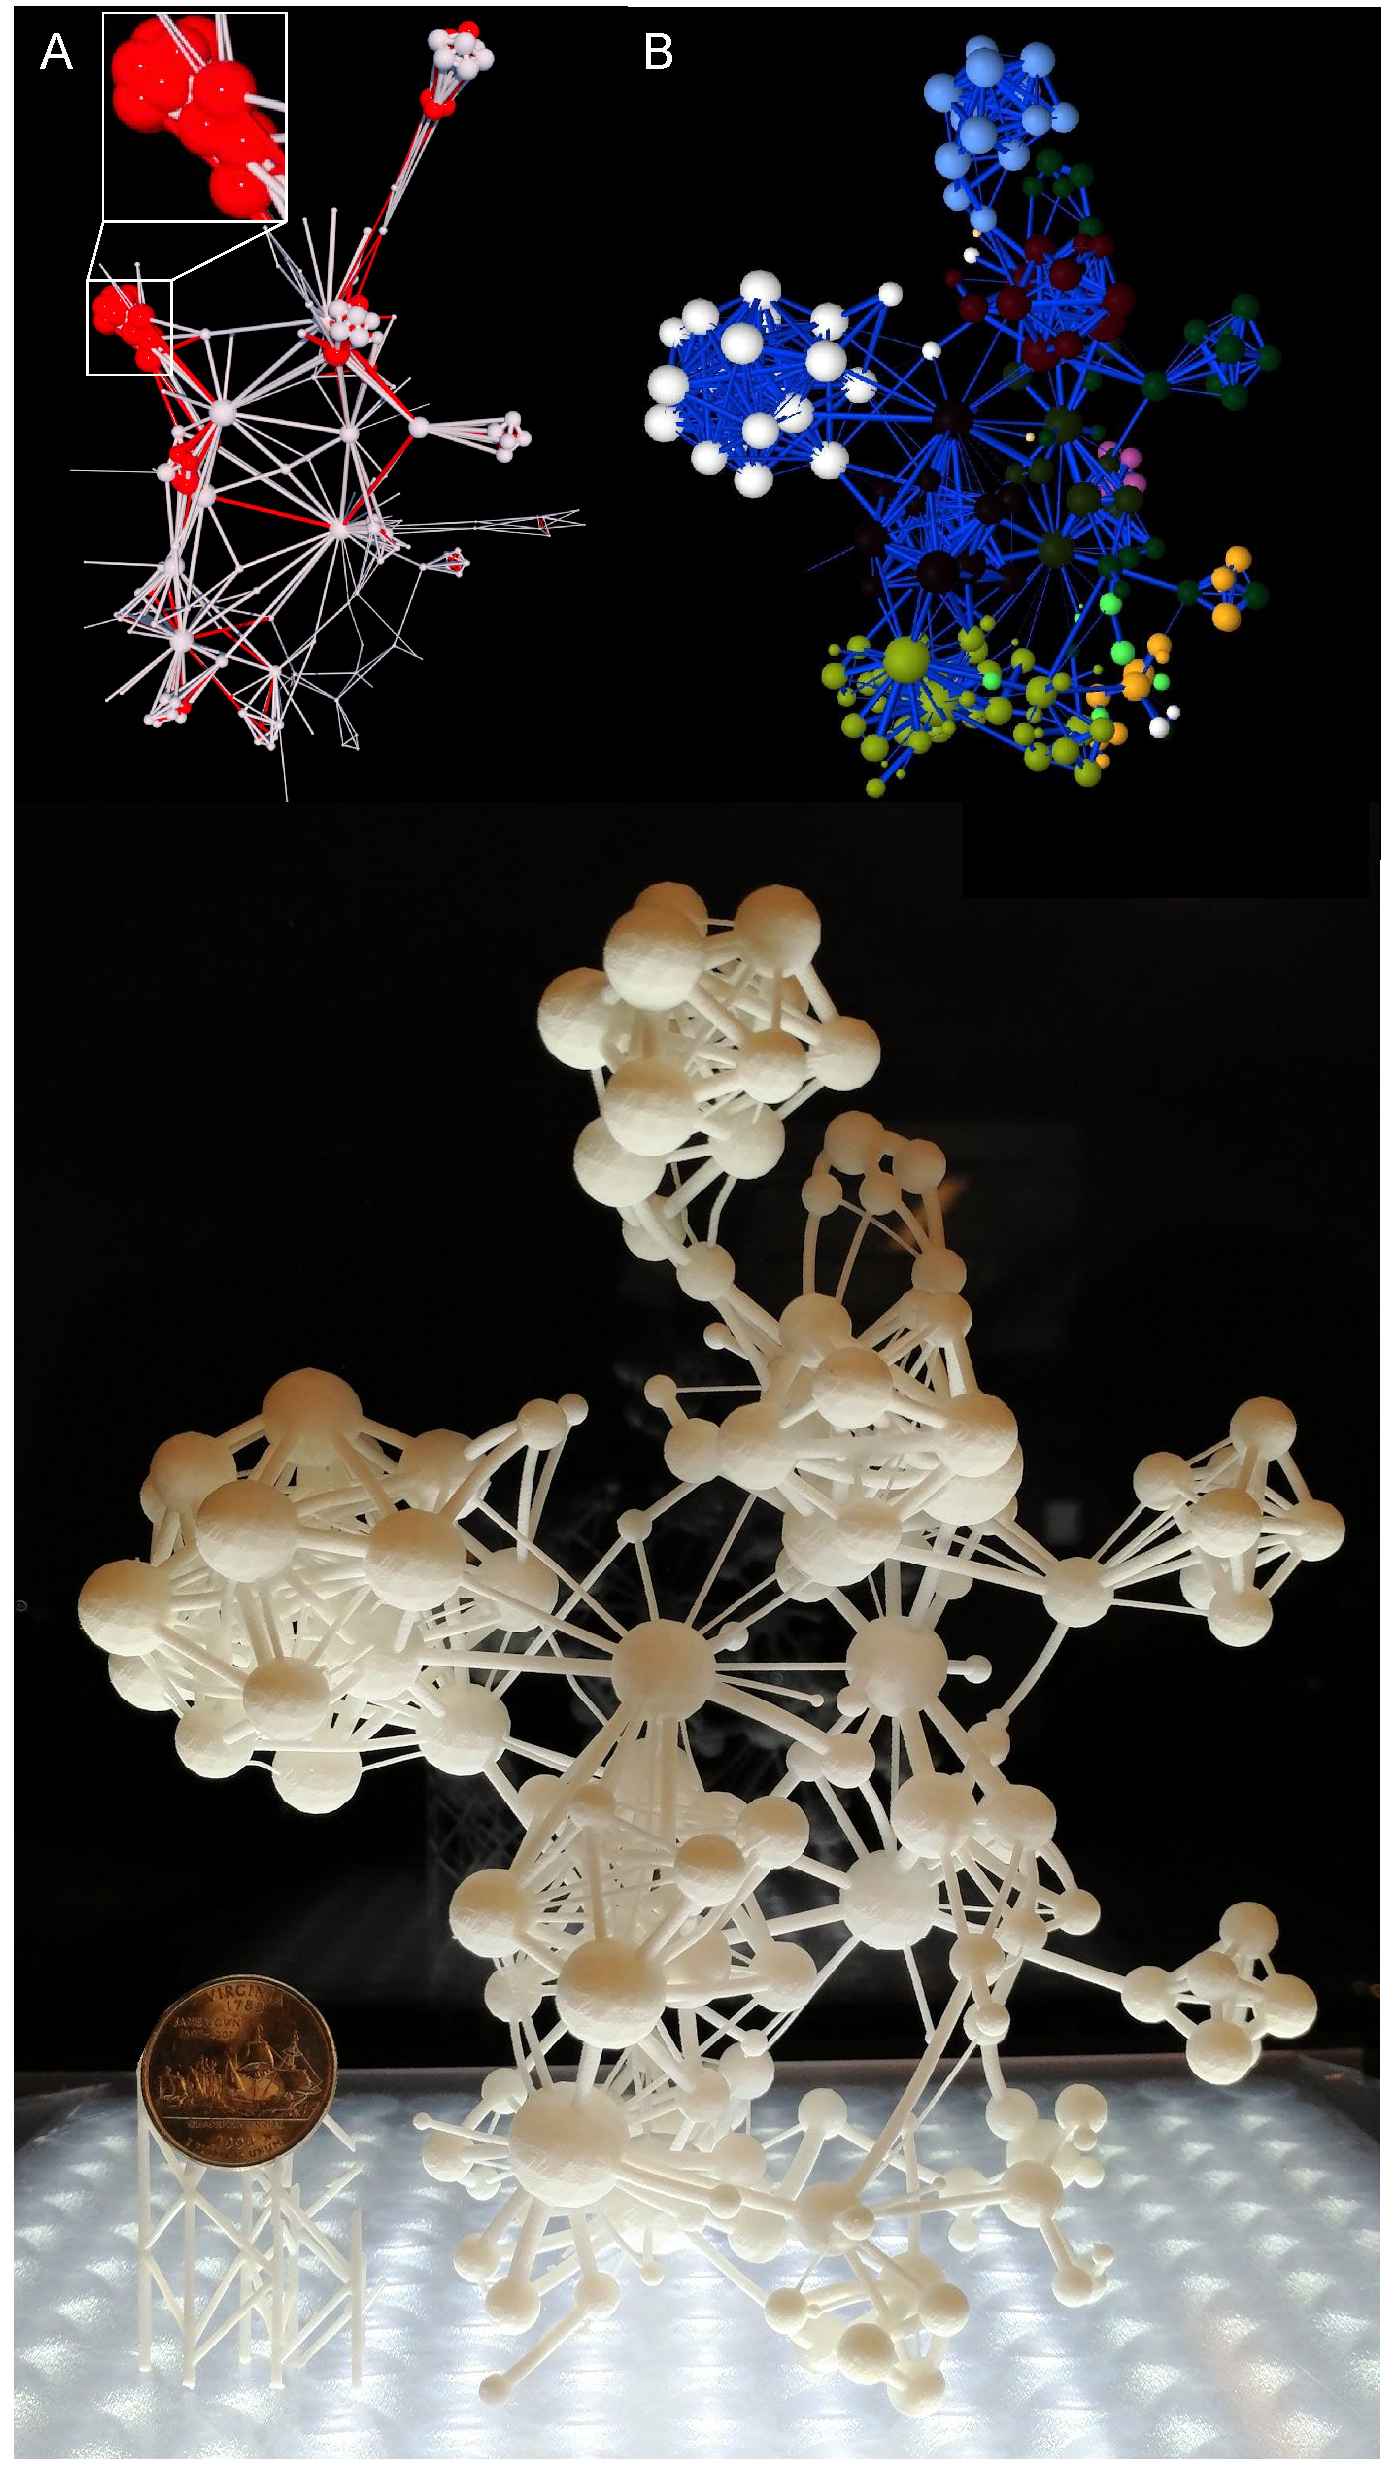
\includegraphics[height=\textheight]{fig-09-19/3D-flavor-111917-3-2.pdf}
\end{figure}
}

In summary, the layout geometry of physical networks is characterized by two distinct phases: a weakly interacting phase, where the overlap between the nodes and links is avoided via local link rearrangements, and a strongly interacting phase, whose layout is shaped by %link crossings.
%{\color{red} ALL topologies in one place} In conclusion, w
%The transition between the two phases is driven by 
excluded volume interactions. 
The layout geometry in the two phases have distinct scaling and physical characteristics: Networks in the weakly interacting phase are solid-like, while
those in the strongly interacting phase behave like a gel. 

Both phases have potentially important applications. 
Indeed, the weakly interacting phase can help us 3D print networks, offering novel opportunities to explore the inner structure of a complex system. 
%Given the cognitive limits of interpreting and experiencing computer images in 3D, it has only limited ability to illustrate its the underlying network's true complexity. 
%The proposed modeling framework can be directly linked to the 3D printing technologies, allowing us to lay out in an optimal manner large networks, and  print them using 3D printers. 
We illustrate this in Fig. \ref{fig:3d-print}, where we first applied FDL to the Flavor Network \cite{ahn2011flavor}.
Given the high link density, 2D visualizations suffer from visual cluttering, making only a fraction of the links visible \cite{ahn2011flavor}. 
A 3D layout offers more clarity, but %we must lay it out in 3D, but in this case, 
given the dense communities, FDL leads to excessive node and link overlaps (inset, Fig. \ref{fig:3d-print}A), obstructing the true wiring of the network. 
Applying FUEL, and choosing $r_L$ so that the layout stays in the weakly interacting phase, the obtained layout geometry reveals the underlying  communities present in the network. 
%As visibility is key for visualization purposes, the weakly interacting phase results in more appealing layouts and is more suited than the strongly interacting phase for visualization (Details on good choice of parameters in SI \ref{ap:params}). 
This layout is amenable to 3D printing, as shown in Fig. \ref{fig:3d-print}B, offering unprecedented opportunities to interact with the network and to directly inspect its inner structure.
%In other words, the modeling framework \eqref{eq:Vfull}--\eqref{eq:Langevin0} could offer an unprecedented opportunity to interact with the structure of large networks, helping us, for example, to visualize disease modules. 
%The addition of weak long-range node repulsion and bundling of links could further enhance the visual aesthetics of the 3D prints, opening up the possibility to better understand complex networks.
Note that the 3D prints must stay in the weakly interacting phase, as in the strongly interacting phase the high link density obstructs the network topology (Fig. \ref{fig:phase-compare}F, J).
%The consequences of the physical constraints in 3D embedding may potentially affect the dynamical and the functional properties of networks. 
In contrast, the strongly interacting phase has direct relevance to the the brain, a three dimensional physical network where the close-packing of the axons is critical to their ability to form synapses \cite{stepanyants2002geometry,rivera2011wiring}. 
%This 
%\cite{azevedo2009equal, herculano2012remarkable, herculano2014brain}
%has been observed to follow 
%is supported by 
Isometric scaling laws observed in rodent brains \cite{herculano2012remarkable} indicate that volume $V_w$ and the area $A_w$ of the white matter relate to each other as $V_w\propto A_w^{1.5}$ \cite{herculano2012remarkable}. 
This implies that in these networks the average neuron length scales as $ \be{l} = V_w/A_w \propto r_L $ with the axon thickness, a behavior present only in the strongly interacting phase % and absent in the weakly interacting phase 
(Fig. \ref{fig:phase-compare}B). 
In other words,  \eqref{eq:Vfull}--\eqref{eq:Langevin0} offers a modeling framework to capture the layout geometry of dense neuronal networks, generating an economic spatial layout %\cite{bullmore2012economy,sporns2004organization,kotter2001connectional}
\cite{bullmore2012economy,sporns2004organization} while respecting the non-crossing conditions each axon must obey \cite{kasthuri12015saturated}.
%As diseases like Multiple Sclerosis \cite{compston2008ms,miller2007ms,miller2005ms}, Schizophrenia \cite{davis2003white,lim1999compromised,sigmundsson2001structural}, Alzheimer's \cite{mudher2002alzheimer,goedert1991tau,goedert1992tau} and Parkinson's disease \cite{bohnen2011white,beyer2006visual,hattori2012cognitive} can arise as a result of disruption of the physical network of myelinated axon fibers in the white matter, our model may prove useful for understanding these diseases. 

%Our model can be utilized for constructing 3D layouts with minimal wiring length.  
%Thus, it can also serve  as a null model for examining wiring efficiency of existing 3D networks, such as brains or artificial networks. 
%By altering the definition  of forces, one can also customize ELI and FUEL to adapt to other scenarios, such as when bundling of links, long-range forces, or varying thickness and sizes are desired. 

% \bibliographystyle{abbrv}
% \bibliographystyle{unsrtnat}

%\newpage
%\newpage

\finV{
\bibliographystyle{naturemag}
\bibliography{mybib}
}{}
\newpage
\newpage


%\end{document}


~
\newpage

%\end{document}

%\appendix
\renewcommand{\thesection}{SI \arabic{section}}
\setcounter{page}{1}
\setcounter{figure}{0}
\centerline{\Huge Supporting Information}

\finV{
\renewcommand{\citep}[1]{}
}{
\maketitle
}

% \setcounter{figure}{0}
% \renewcommand{\thefigure}{SI.\arabic{figure}}

\tableofcontents

%\section{Force-Directed Layout}

\section{Introduction}
Some networks, such as network of neurons in the brain, reside in three dimensional space. 
Links and nodes in these networks occupy space. 
Many aspects of such networks are studied  as part of ``gelation'' processes in polymer physics (see \citep{de1979scaling} chapter IV for instance). 
Gels are like frozen polymers with inter-linking, like vulcanized rubber. But in polymers the ideal situation with maximally stretched links (occupying minimal volume) is not generally of interest, as it is highly unnatural. 
For problems such as organization of the white matter of the brain, however, each long fiber has a cost to produce and thus the system must be very economical.

To understand the structural properties of networks in 3D, we must understand the constraints that being embedded in 3D puts on the network. 
In particular, the layout algorithm used to embed the network in 3D must take the thickness of the links and node sizes into account. 
Most layout algorithms used today are derived from the ``Force-directed Layout'' (FDL) algorithms \citep{davidson1996drawing,kamada1989algorithm}. 
FDL has the benefit that nodes connected to each other are pulled closer and, thus, it clusters nodes that belong to the same network modules \citep{noack2009modularity}. 
However, FDL without modification does not take link thickness into account. 
Here we develop a layout algorithm which is based on FDL, but which allows for efficient layout of networks in 3D, helping us understand the physical properties of such layouts.
By efficient layout we are referring to a layout which aims to minimize the space occupied by the nodes and links. 
In other words, the algorithm tries to find the layout with the shortest links, while avoiding crossings between links or nodes.
We achieve this by defining repulsive forces among links and among nodes. 
As we will discuss below, finding the real optimum of this problem is NP-hard. 
However, using heuristic methods, such as simulated annealing, allows us to find reasonably good layouts in a short time.  

Our main result that networks%\footnote{The networks we consider here are not strongly modular. The results will change slightly if the network consists of distinct modules with different sizes and densities (e.g. networks produced using the stochastic block model.)} 
in 3D will have two main phases: {\em Weakly interacting phase}, where links are very thin, compared to node sizes, and link crossing is rare; {\em Strongly interacting phase}, where links are thick, filling the space, and have to bend and curve significantly to avoid crossing.
The existence of these two phases is observed in various order parameters. 
We use the average link length, average link curvature, as well as the relaxation time for simulations to quantify these two phases and to identify where the transition occurs. 
The details of the definition of link curvature and how we define the relaxation time are given in sec. \ref{ap:phase}.

\outNim{
We start by showing the limitations of FDL when links have thicknesses (\ref{ap:cross}.) 
We show that in FDL the number of conflicts among links generally grows linearly with the link thickness and give a mathematical proof for why that is the case. 
Next, we begin introducing our methodology for modifying FDL to include flexible links.
We construct a potential energy $V$ for this system. 
The optimal layout is found by minimizing the potential energy. 
We show that links that try to find the shortest paths between two points can mathematically be modelled as elastic rubber bands, introducing an elastic potential $V_{el}$ to the potential energy.
Our constraint is that links and nodes are not crossing themselves and each other.
There are many ways for adding this constraint to the system through the potential energy, including hard-core potentials or Lennard-Jones potentials \citep{lennard1924determination}. 
We argue that a Gaussian potential for the repulsion provides a reasonable, differentiable repulsive force, which is well behaved in most numerical simulations and choose it as the basis for the repulsive potentials $V_{NN}$ and $V_{LL}$ for node-node and link-link repulsion, respectively. 

Next, in sec. \ref{ap:np} we discuss how putting this system in a high friction medium forces the dynamics to become a first-order gradient descent, which dissipates the energy of the system until it settles in a local minimum. 
We then discuss in sec. \ref{ap:np}  how this system has a very large number of local minima and that we need to resort to methods such as simulated  annealing to escape unfavorable local minima and find reasonable layouts (\ref{ap:annealing}.)  

A problem that comes up when doing numerical simulations is that discrete simulations of the links assume the links are made of a fixed number of spherical beads. 
Thus, in a link that is stretched a lot the beads will not overlap and two links can cross each other without much repulsive force because of the gaps between the beads.  
This can be fixed by choosing a more advanced repulsive potential for $V_{LL}$, one in which the beads are ellipsoidal, stretching and squeezing when the link stretches or contracts. 
This requires significant change to the Gaussian potential and becomes a version of the Gay-Bern potential \citep{gay1981modification}  (\ref{ap:ell}.)
We then discuss the order parameters that we use to quantify the phases of networks at different values of link thicknesses and node sizes (\ref{ap:phase}.) 
After that we derive the stress tensor for the layouts (\ref{ap:stress}.) We show that in the weakly interacting phase, layouts have stress properties similar to solids, whereas layouts in the strongly interacting phase behave more like a gel. 
Then, we briefly discuss some visualization aspects. 
We calculate how one should choose the relative node and link sizes to allow for visibility of nodes and links, if the goal is to only visualize a network.  
Finally, we discuss aspects of simulating this dynamics and how we wrote our simulation code to be efficient. 
} %%%%

\section{Link Crossing in Layouts with Straight Links \label{ap:cross}}
Before examining the bent links, we first discuss the behavior of link crossing in 3D embedded networks when the link are straight. 
Analyzing the number of crossings as a function of link thickness in FDL yields a linearly growing number of crossings
\outNim{
\footnote{The exact properties of the point where the crossings start is not our primary concern here, but it seems to start at a certain nonzero thickness. 
This sharp phase transition is actually a feature of these connected networks with FDL. 
The transition disappears, as expected, in a system of randomly oriented disconnected links in 3D. 
The length scale at which this phase transition occurs is a function of some dimensionful parameter that can naturally arise from the difference in the form of the repulsive node forces and the attractive forces on the links. We did experiment adding noise to the layout and also randomly switched links around. While these changes increased the slope of the line of the crossings (generally showing more crossings than FDL) they did {\em not} move the point of the phase transition appreciably.}
}(Fig. \ref{fig:crs}.) 
The point where crossings become noticeable depends mostly on the network density parameters, similar to how in self-avoiding polymers the excluded volume depends on the interaction strength. 
\begin{figure}
    %\vspace{4cm}
    \centering
    % \includegraphics[width=.9\columnwidth]{fig-09-19/crs-resolve-0517.pdf}
    % \includegraphics[width=.8\columnwidth]{fig-09-19/crs-resolve-061717.pdf}
    % \includegraphics[width=.7\columnwidth]{fig-09-19/crs-lattice-071917.pdf}
    \includegraphics[width=.7\columnwidth]{fig-09-19/3D-cross.pdf}
    \caption{\scriptsize
    {\bf (A)}  Crossing links for a Barabasi-Albert (BA) network ($N = 20, m = 3$) in space, drawn by FDL. While increasing the link thickness $r_L$, the network occupies more space and crossings increase. 
    {\bf (B)} The plot shows the trend by which the number of crossings increases in a BA network with $N=100, m =3$ laid out in 3D using FDL.
    The number of crossings increases linearly with $r_L$ at first, before tapering off due to finiteness of the network. It can be shown (\ref{ap:cross}) that layouts which result in random link orientations yield such linear trend in the growth of the number of crossings.
    }     
    \label{fig:crs}
\end{figure}
%After all, the nodes can be modeled as interaction points (vulcanization points) on a self-avoiding polymer.  
%Simulations using FDL confirm that link crossings in this layout behave like random uniform layout of nodes in 3D.
Figure \ref{fig:full-range} shows that as we increase the link thickness the number of crossings grows linearly.
\begin{figure}
    \centering
    \includegraphics[width =.99\columnwidth]{figs2/{full-range-n100-m3}.pdf}
    \caption{Left: The behavior of the number of crossings as a function of link thickness. Trivially, once the thickness becomes comparable to the network size (when ``thickness/net. size'' becomes order 1) the crossings saturate and most links cross. The region in which trying to make links avoid each other is much smaller. It extends from zero thickness up to where thickness / net. size is of order $1/\sqrt{N_e}$ with $N_e$ being the number of links in the network. In the BA network with 100 nodes and $m=3$ considered here $1/\sqrt{N_3} \approx 0.06$, which is a safe lower limit for the region where avoiding crossings is possible. Right: a zoomed-in version of the dashed-red box on the lest highlighting this region of validity of avoiding crossings. The legends show a good linear fit to the data up to thickness / net. size = $0.2$.}
    \label{fig:full-range} 
\end{figure}
We show below that randomly oriented cylindrical links will result in a linear trend for the umber of crossings versus link thickness. % that under such a distribution the number of link crossings grows linearly with link thickness\footnote{Assuming cylindrical links. % with circular cross-section.}.


% \newpage
% \appendix


\subsection{Number of Conflicts: Phase Diagram } 
We wish to find the number of crossings as a function of link radius. 
We will divide this radius by $N^{1/3}$ to get the average space per node. 
The number of links should be of order $2N$ because each new node brings in exactly 2 new links. 
Thus, we expect most links to intersect once their radius becomes of order $r/2 $. 
When the thickness is very small we expect there to be very few crossings. In this case perturbing the layout should be able to resolve the crossing. At very high thickness, though we know that the layout may get clogged up so that no perturbation could resolve the crossings. There should be a qualitative difference between these two states.  

\outNim{
\begin{figure}
    {\tiny 
    \begin{tabular}{ll}
    \qquad\qquad BA~(n=200, m=3) & \qquad\qquad BA~(n=500, m=2)\\%[-5pt]
    %{\centering
    \includegraphics[width = .48\textwidth, trim = 0 0 0 1cm, clip]{figs/phase-ba-200-3.pdf}&\includegraphics[width = .48\textwidth, trim = 0 0 0 1cm, clip]{figs/phase-ba-500-2.pdf}\\
    \includegraphics[width = .48\textwidth]{figs/{phase-er-100-0.05-reg-500}.pdf}&\includegraphics[width = .48\textwidth]{figs/{phase-er-300-0.03-reg-500}.pdf}
    %} % centering
    \end{tabular}
    }% tiny
    \caption{Caption}
    %\label{fig:phase}
\end{figure}
}
Simulations of Barabasi-Albert and Erd\"os-Renyi networks layed out in 3D using the Fruchterman-Reingold forced-directed layout seems to suggest that in this setting the qualitative behaviour of these networks for different values of parameters is very similar. 
Figures \ref{fig:simpara},\ref{fig:simrand} and \ref{fig:simfin}  show simulations with parallel, randomly oriented and finite links, respectively. 
The plateau in the number of crossings at large radii is due to the limitation of the optimized algorithm, which partitions the space into smaller boxes and fails when the link radius reaches box size. 
As we can see in Figure \ref{fig:crs-ba-er} the number of crossings in both types of networks and in all four simulations grows linearly with link radius. 
The question is whether this is due to the layouts randomness. 

\begin{figure}
    \centering
    \includegraphics[width=.5\columnwidth, trim = 1.5cm 0 2cm 0, clip]{figs/{phase-er-300-0.03-reg-500}.pdf}\includegraphics[width=.5\columnwidth, trim = 1.5cm 0 2cm 0, clip]{figs/phase-ba-100-3-reg-200.pdf}
    \caption{Simulations of number of crossings in BA and ER networks, when laid out using FDL.
    When plotted in log-log, we see that both networks show a linear trend in the growth of the number of link conflicts as a function of the link thickness. 
    To efficiently calculate the number of crossings, the links are broken into small segment and the space is partitioned into cells. 
    Then, only conflicts within cells with more than one link crossing them are counted. 
    This avoids order $L^2$ computation. }
    \label{fig:crs-ba-er}
\end{figure}



\subsection{Random Crossings}
What is the source of the linear growth of the number of crossings between links with link thickness? 
We show here that it depends a lot on the way the links are arranged in space. 
In particular, we first show that if the links were arranges parallel to each other, but at random distances from each other, the number of crossings among them would grow quadratically with the thickness, inconsistent with the observed trend in FDL. 
Next we show that the observed linear trend is reproducible if the links are either randomly oriented, or even grouped in two groups of parallel links but in two different spatial dimensions (e.g. one stack parallel to the x axis, another to  the y axis). 

\subsubsection{Parallel Links with Random Distances}
For simplicity, let's first consider a number of dots scattered with a random uniform distribution in $d$ dimensional space with a density $\rho$. Suppose we want to grow $d$ dimensional balls around these dots and wish to count the number of balls that overlap. Because of the uniformity, the total number of balls of radius $r$ crossing each other is the number of points that are within less than $2r$ distance of each other, which is
\begin{equation}
    n(r) = \int_0^{2r} \rho(r) dVol=\rho \Omega_{d-1} (2r)^d  \label{eq:nr}
\end{equation}
which scales with the volume of space. In two dimensions, for example, this would mean that the number of circles of radius $r$ crossing each other will be $4\pi \rho r^2$. To compare with the problem of link crossing, if we had parallel cylindrical links in 3D, their cross-section would have been randomly scattered circles in 2D and again the number of crossings should grow quadratically with radius. 

\begin{figure}
    \centering
    \includegraphics[width = .33\textwidth]{figs/para1dir.png}\includegraphics[width = .33\textwidth]{figs/phase-sim-parallel-200-regs-30.pdf}\includegraphics[width = .33\textwidth]{figs/phase-sim-parallel-200-regs-300.pdf}
    \caption{Simulated crossing count of 200 parallel links. One simulation used 30 partition cells in space and the other used 300 cells. In both the number of crossings grows as $r^2$, in accordance with the theoretical expectation. This is in contrast with the linear trend observed in the link crossing of force-directed layouts of random graphs.}
    \label{fig:simpara}
\end{figure}

\subsubsection{Randomly Oriented Links}
Now consider infinite cylindrical links scattered with random orientations in a 3D space. 
Assume that the space occupied by the cylinders has a roughly constant density within cubes of links $d \gg r$. 
Take the cross-section of this space with a flat plane. 
The center lines of the cylinders are uniformly distributed points on the plane and the cross-section of the cylinders are ellipses. 
The ellipses may be very eccentric, but the minor axis, which is also the radius of the largest circle that fits inside the ellipse, is again $r$. Thus, regardless of the eccentricity, if two dots on the plane (the cross-section of center lines of two links) are closer than $2r$ from each other, then the two links will definitely cross. Again, the number of dots less than $2r$ away from each other on any random flat plane grows with $r^2$ and this is only a lower limit for the crossings assuming zero eccentricity for the cross-sectional ellipses.  Therefore the number of link crossings should also grow at least quadratically in 3D.

\begin{figure}
    \centering
    \includegraphics[width = .33\textwidth]{figs/rand-infinite.png}\includegraphics[width = .33\textwidth]{figs/phase-sim-rand-200-regs-100.pdf}\includegraphics[width = .33\textwidth]{figs/phase-sim-rand-400-regs-100.pdf}
    \caption{Simulated crossing count of  randomly oriented links. In both the number of crossings grows as linearly with $r$, in contrast to the parallel link case. This is the same trend as the one observed in the link crossing of force-directed layouts of random graphs.}
    \label{fig:simrand}
\end{figure}

\subsubsection{Two and Three Stacks of Parallel Links along Different Axes}

However, contrary to this argument, as Fig. \ref{fig:simrand} shows, the number of crossings among randomly oriented infinite links does grow only linearly with radius, as it did in the random graph layouts. The same linear trend is observed in finite random links.  

\begin{figure}
    \centering
    \includegraphics[width = .33\textwidth]{figs/rand-finite.png}\includegraphics[width = .33\textwidth]{figs/phase-sim-rand-fin-200-regs-400.pdf}\includegraphics[width = .33\textwidth]{figs/phase-sim-rand-fin-100-regs-400.pdf}
    \caption{Simulated crossing count of  randomly oriented finite links which shows the same linear trend as the infinite randomly oriented links, suggesting that the random orientation is cause for the trend.}
    \label{fig:simfin}
\end{figure}



But there are other simpler examples which also show a linear trend in the growth of the number of collisions. For instance, if we take a number of random parallel links and add a similar number of links that go in a direction perpendicular to to those links the trend becomes linear instead of quadratic, as is demonstrated in Figure \ref{fig:xyz}. The trend is linear for two sets of parallel links, where one parallel set is perpendicular to the other parallel set. The same is true for three perpendicular sets of parallel links. 

\begin{figure}
    \centering
    \includegraphics[width = .33\textwidth]{figs/para2dir.png}\includegraphics[width = .33\textwidth]{figs/{phase-sim-2dir-100-regs-400-rmin=-10}.pdf}
    \includegraphics[width = .33\textwidth]{figs/para3dir.png}\includegraphics[width = .33\textwidth]{figs/{phase-sim-3dir-70-regs-400-rmin=-20}.pdf}
    \caption{Simulated crossing count of 2 and 3 sets parallel links with each set running perpendicular to the other sets. The trend of the number of crossings becomes linear, which is different from the quadratic trend observed in oe set of parallel links in Fig. \ref{fig:simpara} and agrees with the linear trend observed in the link crossing of force-directed layouts of random graphs and in the randomly oriented links in Figs. \ref{fig:simrand} and \ref{fig:simfin}, suggesting that being having components perpendicular to another link may be the key to the linear trend.}
    \label{fig:xyz}
\end{figure}



\subsection{Deriving the Linear Growth of Conflicts}

\begin{figure}
    \centering
    \includegraphics[width =.9\columnwidth]{figs2/crs1.png}
    \caption{\textbf{Left:} The projection of the line through the center of an link \textsf{\textbf{ e1}} on the plane normal to link \textsf{\textbf{ e2}} which crosses the link at point \textsf{\textbf{ n2}}. Because links are randomly oriented, the distance of \textsf{\textbf{ e1}} and \textsf{\textbf{ e2}} is the distance of the blue line from the point \textsf{\textbf{ n2}}. The uniformity then means that the blue lines have uniform density at random angles on the plane and thus their number within distance $d$ is linear in $d$. \textbf{Right:} If links were parallel, the projection of \textsf{\textbf{ e1}} onto the plane would be a point. Thus the distance of the links is the distance of two points on the plane. Uniform spatial distribution in this case means we get uniformly distributed points on the plane and their number within a circle of radius $d$ grows as $d^2$.}
    \label{fig:crs1}
\end{figure}

The number of links within distance $r$ of a point on link $a$  can be found by projecting all links onto the plane to which link $a$ is normal. 
Since the angle distribution is random, we get a uniform distribution of lines on this plane and the number of lines within distance $r$ of a point on a 2D plane grows linear in $r$ (Fig. \ref{fig:crs1}.)

Consider a set of parallel infinite lines distributed uniformly in 2D with linear density $\lambda$ in the direction perpendicular to the lines. Now consider a point $p$ on this plane. The number of links that a circle of radius $r$ centered at $p$ crosses is simply
\[n(r) = \lambda r \] 
and is a linear function of $r$ because only the projection in the direction perpendicular to the lines determines whether or not they cross the circle. 

Now, consider $n$ random lines in a 2D plane with a uniform density (i.e. number of lines passing through a unit square) $\lambda$. Again, the number of lines passing a circle of radius $r$ around a point $p$ grows linearly with $r$. To see this, take a line $l$. Draw the line that passes through $p$ and lands perpendicular to $l$. Say the distance from $p$ to $l$ is $d$. 
This distance determines whether or not $l$ crosses a circle around $p$. Because of the rotational symmetry, if we rotate all lines around $p$ and make all lines parallel to each other we will not change the distribution of their distances from $p$. Since they were distributed uniformly in space, the parallel version will also have a uniform distribution. As we showed above, the number of crossings for the uniformly distributed lines grows linearly with $r$ and thus so does the trend for randomly oriented lines. 
The point $p$ above can be thought of as the center of the cross-section of a link running perpendicular to a plane containing other links. 
Thus, the number of crossings of a link that is perpendicular to a number of other links inside a plane, either parallel links or randomly oriented ones, will grow linearly with the radius of the cross-section of links. 
To see this, take a plane crossing a link (with the link coming out normal to it). 
Project all the other links onto this plane. 
The projections of the centroid of these links will be randomly oriented links on this plane. 
Now, any line that is withing distance $2r$ of $p$ results in a conflict with our reference link. 
If the links are uniformly, randomly distributed in space, the number of links within $2r$ grows linearly with $r$, as argued above. 
This argument only fails if the projections of the other links is not a line in this plane, which only happens if all links are parallel to the reference link. 
We already showed that in that case the crossings grow quadratically. 

%Thus, having a number of links crossing planes containing other links leads to the number of crossings becoming linear in $r$. 
%The 3D space can always be stratified in arbitrary parallel planes and as long as there exist a roughly equal number of links going in at least two perpendicular directions, the points found from the crossing of the center lines of an link with a plane containing another set of links always qualifies for the arguments above, even if the link isn't exactly perpendicular to the plane. 

Thus, having links that have components in at least two perpendicular directions in 3D leads to a linear trend in the number of crossings as a function of $r$.  


\subsection{Finding Overlapping Links}
Consider two straight links $A$ and $B$. Denote the two vectors pointing to the endpoints of the two links by $A_1,A_2$ and $B_1,B_2$. Define the $a= A_1 - A_2$ and $ b= B_1 -B_2$ which are parallel to the lines connecting the two endpoints of each link. The links are cylinders of diameter $d$. We wish to find whether or not the two links intersect, i.e. whether the two links come closer than a distance $d$ of each other. The shortest distance of the two vectors is $a \times b$, since this is perpendicular to both $a$ and $b$. Define
\[c = a\times b\]
we can decompose $ a$ to its components parallel and transverse to $b$ 
\begin{align}
a &= a_\parallel \hat{b}+ a_\perp (\hat{b}\times \hat{c})\cr
a_\parallel &= a\cdot \hat{b}, \cr
a_\perp &= a \cdot (\hat{b}\times \hat{c}) = \hat{c} \cdot (a\times \hat{b})= {|c|\over |b|}
\end{align}

\subsubsection{Measuring Link Distance}
Consider the plane $P$ spanned by $b$ and $c$ and containing the link $B$. The unit vectors $\hat{b}$ and $\hat{c}$ form an orthonormal coordinate system for this plane and any point on the plane can be written as
\[x_p = x_m \hat{b}+ x_c\hat{c}\]
The plane itself is defined through the normal vector 
\[\hat{n}= \hat{b}\times\hat{c}\]
and any multiple $p\hat{n}$ of $\hat{n}$ from the origin intersects the plane.
When $ a$ and $b$ are not parallel to each other, $a$ will cross the plane $P$ at a single point. The projection of link $A$ onto $P$ is a line parallel to $B$. Therefore we can use the following to find the distance between the two links. We will first pick one endpoint from each of $A$ and $B$. The vector connecting the two
\[d = A_1-B_1\]
is a vector whose projection of the vector $c = a\times b$ is perpendicular to both $a$ and $b$ and thus also to the projection of $a$ onto $P$. Since on $P$ the projection of $a$ is parallel to $b$, the magnitude of the projection $d_p$ of $d$ onto $P$ is the minimum distance between the two links. Thus we have
\[|d_p| = d \cdot \hat{c}\]

\subsubsection{Caveat}
The above mentioned $d_p$ is the least distance of the two links only if $A$ crosses the plane $P$. Otherwise, one of the endpoints will be the closest point to the other line and we need a different strategy. Let's first figure out a way to see if $A$ crosses $P$ or not. To this aim we will look at the projections of $d_1= A_1-B_1$ and $d_2 = A_2 - B_2$ along the normal $\hat{n} $. Regardless of which endpoints of $A$ are being connected to which on $B$, if the projections of $d_1\cdot \hat{n}$ and $d_2\cdot \hat{n} $ have the same sign it means $A$ did not cross $P$ and if they have opposite signs or one is zero $A$ will have crossed $P$. Thus  
\[\mbox{if: } (d_1\cdot \hat{n})(d_2\cdot \hat{n}) >0 \quad \Rightarrow  A\mbox{ not crossing }P\]
And so the closest point on $A$ to $B$ is one of $A$'s endpoints. Similarly, we need to check if $B$ crosses the plane spanned by $A$ and $\hat{c}$. If not, the closest distance of the $A$ and $B$ will be one of their endpoints to each other. 


\section{Elastic Link Models: ELI and FUEL}
Our main goal is to understand the volumetric constraints on embedding networks in 3D. 
To achieve this we propose a simple model that minimizes the length of links, while avoiding link crossing. 
We will begin by deriving  mathematically how to find the shortest path between two points, in presence of obstacles, showing that it is equivalent to stretching a rubber band between them.
Next, we define smooth alternatives to hard-core repulsion to define repulsive forces among links and among nodes to make crossings energetically unfavorable. 
We then combine all the potential energy terms and derive the equations of motion in a strongly dissipative medium, to make sure the system moves to a locally minimum energy state. 

\outNim{
\begin{figure}
    \centering
    \includegraphics[angle=0, width = .5\columnwidth, trim= 0 0 12in 0 ,clip]{figs1/{sud05}.pdf}\includegraphics[angle=0, width = .5\columnwidth, trim=  11.5in 0 .5in 0 ,clip]{figs1/{sud05}.pdf}
    \caption{methodology}
    \label{fig:forces}
\end{figure}

\begin{figure}
    \centering
    \includegraphics[angle=0, width = .8\columnwidth]{figs1/{sud05}.pdf}
    \caption{methodology}
    \label{fig:forces}
\end{figure}
%} %% out
\begin{figure}
    \centering
    \includegraphics[angle=0, width = .5\columnwidth]{figs1/{method1}.pdf}\includegraphics[angle=0, width = .5\columnwidth]{figs1/{method2}.pdf}
    \caption{methodology}
    \label{fig:method}
\end{figure}
} %% out

\subsection{Equivalence of Shortest Path and Stretched Rubber Band\label{ap:affine}}
%#  Numerics of the geodesics
To find a globally optimum geodesic, be it in flat or curved space, one has to check many different paths and locally optimize them. 
A locally optimized path, meaning every segment is as short as possible, is a geodesic. 
But in curved space there exist many geodesics connecting two points. 
This is because the geodesic equation is a second order ODE and different initial velocities may exist which make the geodesic cross the same final point in space. 
%\subsection{The rubber band model}
Denote the components of the metric of the space by $g_{\mu\nu}$. 
Heuristically, since a geodesic is locally the shortest path, a simple way to find geodesics between points should be to assume that they are stretched rubber bands. 
This assertion can be made rigorous. 
The key point is that for a geodesic we are minimizing the total path length locally, which means that we are minimizing the action
\begin{equation}
    S[\gamma;a,b] =\int_\gamma dt \sqrt{ g_{\mu\nu}(x) {dx^\mu(t)\over dt}{dx^\nu(t)\over dt}}  \label{eq:Sdl}
\end{equation} 
where $\gamma$ denotes the geodesic path. 
The energy for a rubber band has a similar form, but it lacks the square root 
\begin{equation}
E[\gamma;a,b]= {k\over 2}\int_\gamma g_{\mu\nu}(x) {dx^\mu(t)\over dt}{dx^\nu(t)\over dt} dt \label{eq:Ekx2}
\end{equation}
But if the parameter $t$ is itself an ``affine parameter'' (e.g. using the actual proper length element $dl = dS$ as the parameter, with $S$ being the action above), %for example the proper length which is the same as the action $S$ above, 
we can   show that the equations of motion derived from $S$ and $E$ become the same. To see this, we will derive the Euler-Lagrange equations from varying $S$ and $E$. First define
\[dl \equiv \sqrt{ g_{\mu\nu}(x)dx^\mu(t) dx^\nu(t)}, \]
and for convenience $f\pr{x} \equiv {kx^2/ 2}$ so that $E = \int f(dl/dt) dt $. Varying $S$ yields
\begin{align}
    \delta S =& \int dt \delta \pr{{dl \over dt}} = \left.{\ro \dot{l} \over \ro \dot{x}^\mu} \delta \dot{x}^\mu\right|_{t_0}^{t_f} -\int dt \delta {x}^\mu  {d\over dt} \pr{{\ro \dot{l} \over \ro \dot{x}^\mu}} 
\end{align}
where the first term is a boundary term and vanishes because $\delta \dot{x}^\mu = 0 $ at the boundaries.  
From varying $E$ we have
\begin{align}
    \delta E =& \int dt {df(\dot{l}) \over d\dot{l}} {\delta \dot{l} \over \delta x^\mu} \delta x^\mu \cr
    =& \left.{df(\dot{l}) \over d\dot{l}}{\ro \dot{l} \over \ro \dot{x}^\mu} \delta \dot{x}^\mu\right|_{t_0}^{t_f} -\int dt \delta {x}^\mu  {d\over dt} \pr{{df(\dot{l}) \over d\dot{l}} {\ro \dot{l} \over \ro \dot{x}^\mu}} \cr
    =& -\int dt \delta {x}^\mu \left[ {\ro \dot{l} \over \ro \dot{x}^\mu} {d\over dt} \pr{{df(\dot{l}) \over d\dot{l}}} + {df(\dot{l}) \over d\dot{l}} {d\over dt} \pr{ {\ro \dot{l} \over \ro \dot{x}^\mu}}\right] 
\end{align}
In the last line, if we only had the second term minimizing $E$ would require the same equation as minimizing $S$. The first term here contains 
\[{d\over dt} \pr{{df(\dot{l}) \over d\dot{l}}} = k {d \dot{l}\over dt} ={d^2 l \over dt^2} \]
If the parameter $t$ is an affine parameter, say $ t\propto l$, i.e. proportional to the proper length $l$ itself, this term is proportional to $d^2 l / dl^2 = 0$  and would vanishes. So, an affinely parametrized geodesic and the energy function of a rubber band with the same parametrization yield the same equations of motion. Thus, we can replace the problem of finding geodesics between two points with the problem of finding minimum energy configurations of a stretched rubber band connecting the two points. 
%This means that an affinely parametrized geodesic is in fact a minimum energy stretched rubber band. 
The difference in initial velocities of an object following the geodesic, which leads to having multiple geodesics connecting two points, is related to having different spring constants $k$. %Consequently, we will find geodesics by allowing rubber bands to approach their minimum energy states.

\outNim{
\subsection{Other Links}

We will implement the curved-space rubber-band similar to flat space. The repulsive force from other links is a function of their geodesic distance, but that is hard to calculate in curved space. Since we assume the force to be short-ranged, we will use a constant metric, based on the midpoint between the two points to calculate the distance between the two points and won't use accurate geodesic distance. 

Also, we will add this repulsive force directly as a force on the l.h.s. of the geodesic equation and won't try to incorporate it into the metric and derive perturbed Christoffel symbols. 
Thus we will only need to define a global metric function.  

}


\subsection{Elastic Links}
As is known about geodesics \citep{novikov1984}, and discussed in appendix \ref{ap:affine}, the problem of minimizing the length of links can be mapped to stretching elastic rubber bands between points in space\footnote{The trade-off is that we lose re-parametrization invariance. The energy equation has a fixed parametrization $ds_l$ which is an affine parametrization of the path.}. The contribution of the stretched rubber band model of link $l$ to the total energy is
\begin{equation}
  E_l[\gamma_l] = {k\over 2}\int_{\gamma_l} ds_l {d\vec{x}_l\over ds_l} \cdot {d\vec{x}_l\over ds_l}, \label{eq:El}
\end{equation}
where $d\vec{x}_l/ds_l$ denotes the tangent vector to link $l$ (along the line through the center of the tube), $\gamma_l$ is the path of the link, and $k$ is the spring constant. 
The energy is obviously a function of the path $\gamma_l$. 
The full elastic potential $V_{el}$ of the system is
\begin{equation}
    V_{el} = \sum_l E_l
\end{equation}

The rubber links will occupy some space and exert a strong repulsive force on each other. Within one link, however, we will only assume no repulsive interactions. This allows the links to shrink to their minimal length under the elastic force of the stretched rubber band model and assume the equilibrium length of the band the be zero to allow for maximum shrinking. 

\subsection{Repulsive Potential\label{ap:repel}}

For large molecules one usually uses a potential ansatz like the Lennard-Jones potential $V \sim (r_L/r)^{12} - (r_L/r)^6 $ to simulate the van der Waals interactions, which is weakly attractive at large distances and strongly repulsive at short distances of order $r_m$. Since we are not concerned with molecules here but rather spatially embedded networks in general, we will not assume any attractive force between links and only assume there is a strong repulsion once link walls get close to each other. The simplest way to model this would be a repulsive force $F = -\del V$ that grows quickly once links get closer than twice the link thickness. In the ideal case, the force is infinite when the two touch or have distance less than twice the thickness. But a force coming from an infinite potential, does not behave well in numerical simulations. A remedy is to simply not allow segments to move into each other by fixing minimum distance. But a better strategy numerically is to ``regularize'' the potential by replacing it with a finite potential that achieves approximately the same results. 

The simplest regularization would be to replace the wall potential with a steep incline
\[V \sim \begin{cases} -A(r -r_L) & r< r_L \\
0 & \mbox{otherwise} 
\end{cases}\]
with $A$ being large compared to $1/\delta t$. 
But again, from the numerical point of view this has the problem that the force is exactly zero at $r_L+\eps$ and nonzero and large at $r_L - \eps$ which causes numerical errors and irregular behavior. Also from the physics perspective this potential is bad because the direction of the force is ambiguous at the origin. A physically meaningful force would either become infinite so that the other particle could never reach $r=0$ or it would go to zero so that the force direction wouldn't matter at $r=0$
\[\mbox{Physical: } \lim_{r\to 0} F(r) = 0 \quad \mbox{or}\quad \infty \]
Since $F(r)\to \infty$ is again numerically problematic, the only choice is $F(0) = 0$. To get $F(0) = 0$ we may choose the potential to be an inverted parabola like
\[V \sim \begin{cases} A(r -r_L)^2 & r< r_L \\
0 & \mbox{otherwise} 
\end{cases}\]
Of course we can also take $V\propto 1/r^n$ 
and regularize it to something like $1/(r^n+\eps)$, but the resulting force is long-range, because it falls like a power-law. We may again cut this force off beyond $r_L$, but all these choices make the repulsive force harder to control and make assuring that the links stay outside of $2r_L$ distance harder to implement. 
Also, to fix the numerical force discontinuity issue when $r\to r_L$ we have to have a potential which is smooth at $r_L$. Thus instead of the patchwork encountered above, the numerically  sane 
alternative that provides both a controlled, localized force and with an adjustable amplitude without having to patch different functions together and without the need for regularization is the Gaussian potential. 
The Gaussian provides a force which is smooth everywhere, including at the origin and is therefore an ideal choice for numerical simulations. 
The thickness of the links will then be twice the width of the Gaussian potential and the amplitude is the strength of the repulsion.  

\begin{figure}
    \centering
    \includegraphics[width=.9\columnwidth] {figs2/gauss-pot.pdf}
    \caption{Comparison of the linear incline and the Gaussian potential. While looking similar in shape, the force from the Gaussian is much more well-behaved at $r= r_L$ and $r=0$ and is better suited for numerical analysis. }
    \label{fig:gauss}
\end{figure}

\subsubsection{Gaussian-type Repulsive Force}
%We will argue in appendix \ref{ap:repel} 
We argued above
that one of the most appropriate choices of repulsive potential which is tailored for our purpose is the Gaussian potential. 
We will assume that every line segment in one link has a repulsive Gaussian interaction with every segment of another link. Consider a segment of link $a$. Denote the value of the length parameter parametrizing the path $\gamma_l$ of the link by $s_l$. The tangent vector to this infinitesimal segment $d\vec{x}_l(s_l)$ interacts with segments of other links via
\begin{equation}
dV_{lm} = %|d\vec{x}_l| |d\vec{x}_m| 
ds_lds_m
A \exp\left[- {|\vec{x}_l-\vec{x}_m|^2 \over 4 r_L^2}\right]\label{eq:dVij}.
\end{equation}
Here $A$ is the amplitude of the force and $r_L$ is the cross-sectional radius of the links.
Thus, the total interaction between segments of $a$ and $b$ is found by integrating over the paths of the two links
\begin{equation}
V_{lm}[\gamma_l,\gamma_m] = \int_{\gamma_l} \int_{\gamma_m} dV_{lm} \label{eq:Vij}
\end{equation}
which depends on the two paths $\gamma_l$ and $\gamma_m$.  
The full link-link repulsion potential is then
\begin{equation}
    V_{LL} = \sum_{l\ne m} V_{lm}
\end{equation}
Other potentials of the form $\exp[-|\vec{X}_i-\vec{X}_j|^n/(2r)^n]$ with $n>2$ may also be used. 
The higher the $n$, the steeper will be the potential. 


\subsection{Node Repulsion}

To add node dynamics to the system, we will define the node positions $\vec{X}_i$ as dynamical variables. 
The full node-node repulsion potential is \begin{equation}
V_{NN} = \sum_{i\ne j }V_{ij},\qquad  V_{ij} = %|d\vec{x}_l| |d\vec{x}_m|
A_N \exp\left[- {|\vec{X}_i-\vec{X}_j|^2 \over 4 r_N^2}\right]\label{eq:VIJ0}.
\end{equation}
where $i,j$ are node indices, $A_N$ is the amplitude of the repulsive potential and $r_N$ is the node radius. 

The force from the links on the nodes does  not come from a new potential. 
It is, in fact, contained inside the elastic potential of the links, %$dV_{ij}$ in \eqref{eq:dVij}, 
as the endpoints of the links is attached to the nodes. The only point is that we will allow nodes to be dynamic, instead of fixed. We denoted the tangent vector along link $a$ by $\vec{v}_l(l) = d\vec{x}_l(s_l)/ds_l $. To couple the links with their corresponding nodes we simply need to add a minimal coupling interaction between the end-point tangent vectors $\vec{v}_l (0)$ and $\vec{v}_l (s_l)$ with the nodes they attach to. Here $s_l$ denotes the final value of the affine length parameter $s_l$ for link $a$. The potential for this interaction looks like\footnote{In general each term could have a different coupling coefficient, but that degree of complexity is unnecessary here.}
\begin{align}
   V_{NL} & =c\sum_{i=1}^N \vec{X}_i \cdot \sum_{a\in <i>}  \vec{v}_l\pr{l^{(\mathrm{end})}_l}
\end{align}
where $<i>$ denotes the set of indices of links connected to node $i$ and $l^{(\mathrm{end})}_l$ is either $0$ or $s_l$ depending on which end of link $a$ is attached to node $I$. We will assume $c =1$. We will also assume that the mass and friction constant for the nodes is such that the $\lambda_N$ in the Langevin equation is of the same order as the $\lambda$ for the link segments in \eqref{eq:Langevin0}. 

\subsection{Full Potential Energy}
In summary, the total potential energy of the system becomes
\begin{align}
    V &= V_{el} + V_{NL} +V_{NN} + V_{LL} \cr 
    &= {k\over 2}\sum_l\int ds_l \left|{d\vec{x}_l\over ds_l} \right|^2 + 
    \left. k\sum_{i=1}^N  \sum_{l\in <i>}  \vec{X}_i \cdot{d\vec{x}_l%\pr{l^{(\mathrm{end})}_l} 
    \over ds_l}\right|_{s_l = s_l^{(\mathrm{end})}}
    \cr
    &+ A_N\sum_{i\ne j}  \exp\left[- {|\vec{X}_i-\vec{X}_j|^2 \over 4r_N^2}\right]+A_L\sum_{l\ne m} \iint ds_lds_m 
    \exp\left[- {|\vec{x}_l-\vec{x}_m|^2 \over 4 r_L^2}\right] ,
 \label{eq:Vfull1}
\end{align}
where $V_{el}$ is the total elastic potential of all links $l=1,...,L$. 
Each link is modeled as an elastic cylinder with radius $r_L$, experiencing both internal elastic forces and short-range external repulsive force from other links and nodes. $V_{NL}$ captures the node-link interactions at link endpoints;
the non-crossing condition is ensured by a short-range repulsive force in
$V_{NN}$  (node-node interaction)  and  $V_{LL}$ (link-link interaction) modeled as short-range Gaussian potentials whose strength is set by $A_N$ and $A_L$. 
In \eqref{eq:Vfull1} $s_l$ is the length parameter of link $l$ and  $\vec{x}_l(s_l,t)$ represents the position of a point along the center of the link at time $t$;
$s_l^\mathrm{(end)}$ is the parameter value at the endpoints of link $l$;
$l\in <i>$ represents the set of links connected to node $i$; 
$\vec{X}_i(t)$ is the position of node $i$; $r_N$ is the range of the node-node repulsive force; $k$ is the elastic constant of the links.

\subsection{Dynamics and Minimization of the Potential Energy\label{ap:eom}}
The total potential energy for the links, which is a function of the set of paths $\{\gamma \} $ that they take, is given by
\begin{equation}
V[\{\gamma\}] = V_{el} + V_{LL} = \sum_l E_l + \sum_{lm} V_{lm}. \label{eq:V}
\end{equation}
%where $\{\gamma\}$ denotes the set of the paths taken by the links. 
To find the ground state of this system, i.e. optimal static configuration, we can introduce  strongly dissipative dynamics in the system. 
As we show below, this will make the equations of motion effectively first order, gradient descent equations.  
%This way, instead of having to solve complicated coupled differential equations, we can simulate the dynamics and simply let the system converge to its equilibrium state. 

Consider a point $\vec{x}_l(s_l(t))$ on link $a$ where the length parameter has value $s_l(t)$ and at time $t$. We can introduce a kinetic energy term to the energy which is the sum of the kinetic energies of all infinitesimal segments.
A segment of length $ds_l$ will have a mass $\lambda ds_l $, $\lambda$ being the linear mass density, and thus its kinetic energy is
\[dK_l = \lambda ds_l \left|d^2 \vec{x}_l \over dt \right|^2.\]
Summing over all segments we get $K_l[\gamma_l] = \int_{\gamma_l} dK_l$. Friction terms for an infinitesimal segment will have a similar structure. If we assume we are in a viscous medium and that the amount of friction is simply proportional to the length, in the equation of motion for a segment of length $dl$, kinetic friction $f_k$ appears as 
\[df_k(l,t) =\eta ds_l {d\vec{x}_l(l,t)\over dt}.\] 
Since the potential depends on both time $t$ and the length parameters $s_l$, the equations of motion are more complicated than the usual particle equations of motion. 
We can think of the position vectors $\vec{x}_l (s_l,t)$ as three component (in 3D) fields whose parameters are $s_l,t$. 
The equations of motion are derived the same way as for fields. 
We have a potential energy density that is a function of both the field $\vec{x}_l$ and its derivative with respect to $s_l$  $\vec{v}_l \equiv d\vec{x}_l/ds_l$. 
The equation of motion therefore includes partial integration with respect to $s_l$. 
In summary, if we denote components of $\vec{x}_l$ by $x_l^\mu$, we have 
\begin{align}
    \mbox{EoM}:\quad \lambda {d^2 x_l^\mu \over dt^2} +\eta {dx_l^\mu \over dt} & =  -{\ro V \over \ro x_l^\mu} + {d\over ds_l} {\ro V \over \ro v_l^\mu}.   \label{eq:Langevin}
\end{align}
The first term on the right is the familiar $\del_{x_l} V$ and will be nonzero only for the repulsive potential $V_{lm}$. But the second term acts on the internal elastic potential and yields \[{d\over dl} {\ro V \over \ro v_l^\mu} = k {d^2 x_l^\mu \over ds_l^2}.\]  
This is measuring the change in lengths of the segments from one point to another. The reason is that when a rubber band is stretched uniformly, the internal points will not move relative to each other because all forces in all pieces are the same and they cancel out. There will be a non-zero force, and hence movement along the rubber band, only if there is a change in the segment tangent vectors $\vec{v_l} = d\vec{x}_l/ds_l$ in adjacent segments, as they measure length vectors along the band.



\outNim{
{
\color{red} !!! Needs correction!!!}
\[K_l [\gamma_l]\equiv \int_{\gamma_l} dl \left|d^2 \vec{x}_l \over dt dl\right|^2.\]
} %%%% 

We can now derive the Euler-Lagrange equations for a segment of length $ds_l$ around this point using the action $S = K- V$. To do so, we need the variations with respect to both the position of the points $\vec{x}_l$ and the tangent vector $\vec{v}_l \equiv  d\vec{x}_l/ds_l(t)$. They read 
\begin{align} 
{\delta S[\{\gamma\}] \over \delta \vec{x}_l} : \quad {d^2 \vec{x}_l \over dt^2 }  
=&  \vec{\del}_{{x}_l} V[\{\gamma\}]- {d\over dl} \vec{\del}_{{v}_l} V[\{\gamma\}] \cr
=& -k {d^2\vec{x}_l\over ds_l^2} + {A\over 2 r_L^2}\int_{\gamma_m} ds_m
 (\vec{x}_l-\vec{x}_m)\exp\left[- {|\vec{x}_l-\vec{x}_m|^2 \over 4 r_L^2}\right]
\end{align}


To allow the system to quickly converge to a local minimum of the potential we will assume strong friction, meaning that, if the observation time is $\tau$, we will assume $\lambda \tau \gg 1$ and will discard the acceleration term. So in the end the equation whose dynamics we will simulate to find local minima of this system is 
\begin{equation}
\eta {d \vec{x}_l \over dt }  
= - \vec{\del}_{{v}_l} V + {d\over ds_l} \vec{\del}_{{v}_l} V\label{eq:Langevin1}.
\end{equation}
Once the dynamics stops, all forces vanish and we will end in some local minimum. 


\subsection{Curse of Local Minima \label{ap:np}}
Notice that the equations above stop the dynamics at any local minimum. 
Similar to many other coupled systems, such as spin glasses \citep{parisi2002physical,pelissetto2002critical}, the energy landscape of this system is rough and consists of exponentially many locally optimum states which may themselves lie far from the globally optimum configuration. 
%One can see this fact by assuming a configuration where one link goes around the whole network, instead of going as  straight as possible toward its target. Starting from this situation we can still run the dynamics and shrink all rubber bands as far as possible. The final state is an equilibrium state and a local minimum of energy, but its total energy will be much higher than the global optimum. 
Therefore, we will use Simulated Annealing to allow the system to escape local minima and find close-by, potentially lower local minima.  

The amplitude of repulsion among links, as well as the choice of number of segments  play a role in how well the system can manage to get out of local minima. 
Choosing a high number of link segments to mimic the continuity of links, will make it harder for links to pass through each other. 
Subsequently, tunneling between local minima gets more difficult and the layout will almost always get stuck in a local minimum, where part of the lattice is twisted, or has a kink.


\subsubsection{Simulated Annealing and Vast Local Minima \label{ap:annealing}}
The trick is to add some thermal noise to the system. In our case, we can think of the thermal noise literally as thermal fluctuations of the links. We start by assuming that the positions of link segments are only known as a statistical average and that they fluctuate. Thus we replace

\[ds_l(t) \to \be{ds_l(t)}_{T(t)} \]
where $T(t)$ is the temperature of the system at time $t$. 
The amount of fluctuation will be proportional to the temperature and the energy of the path. Thus, we have to sum over all paths that the links take and we have to weight each path by the Boltzmann factor based the energy of the path. If we discard the kinetic part of the energy because of high friction, the expression for the Boltzmann weight becomes similar to the ``world-line formalism'' of polymers. Denote the sum over all possible paths $\gamma_l$ for link $a$ by $\int [d\gamma_l]$. The partition function for this system, assuming strong friction, is given by
\begin{align}
    Z[\beta] & = \int \prod_l [d\gamma_l] \exp\left[-\beta V[\{\gamma\}]\right],  
\end{align}
with $\beta = 1/T$. 
This is closely related to the world-line formalism of polymer partition function \citep{des1974lagrangian}. 
Now, instead of the original Langevin equations, the expected values of variables satisfy these equations
\begin{equation}
0= \be{\lambda {d \vec{v}_l \over dt } + \vec{\del}_{{v}_l} V} = \int \prod_l [d\gamma_l] e^{-\beta V[\{\gamma\}]}\pr{\lambda {d \vec{v}_l[\gamma_l] \over dt } + \vec{\del}_{{v}_l} V[\{\gamma\}]}  \label{eq:Langevin2}.
\end{equation}

Note, however, that this equation only makes sense if we are close to equilibrium because we are using an equilibrium Gibbs distribution. That is the thermal fluctuations must happen at a time-scale that is much faster than the time-scale of the dynamics so that the thermodynamic averaging makes sense. When this is not the case, the problem still makes sense as a non-equilibrium system, but the expected value equation above will deviate significantly from zero if the temperature is not extremely small. In other words, even when the dynamics takes the system to the vicinity of a local minimum we have 
\begin{equation}
\be{F(t)}_{T,dt} \approx F \pm \delta t {|\ro_t E|\over \sqrt{T}} \sigma(F)_{T,dt}, \label{eq:fluct}  
\end{equation}
where $F$ is the value without thermal fluctuations (i.e. at $T=0$), and $|\ro_t E|$ is the rate at which the system's energy is changing. This means that when the system is not at equilibrium the thermal average taken over a period $dt$ will fluctuate in accordance with the rate of energy change. 
Since the global minimum cannot be calculated analytically in general, we don't have to worry about near equilibrium description and running the annealing schedule should yield good enough configurations because the fluctuations in \eqref{eq:fluct} allow the system to jump over barriers in the potential energy that are smaller than the $\sigma_F$ term in \eqref{eq:fluct}. 

The setup described above is mathematically similar to that of interacting elastic polymers, or more generally fluctuating manifolds in \citep{mezard1991replica} with imaginary noise. % and similar problems like the landscape problem, i.e. many local free energy minima, exist here as well. 

\subsubsection{Annealing Schedule}
We start cooling the system with an exponential cooling schedule and once it ``freezes'' as $T \to 0$, we will examine the energy. Simulated annealing is not guaranteed to find the global optimum, but it generally finds states that are much better than a local minimum attained by a fixed initial condition\footnote{ The reason is that the thermal fluctuations allow the system to explore large areas of the energy landscape and the gradient descent introduced as the dynamics will help the system fall into the lowest minimum within that large phase space area. The fluctuations, which allow the system to overcome small barriers between local minima, are effectively smoothening the energy landscape in the sense of \eqref{eq:fluct}. }. This is related to the fact that the thermal fluctuations may be seen as renormalization of the free energy (similar to the discussion of chapter XI of \citep{de1979scaling}) which gets rid of small local dents in the potential energy landscape.  

Thus, all we need to do is add thermal noise to the system during the dynamics and gradually decrease the level of the noise, hence decreasing the temperature and ``anneal'' the system. We choose the schedule of the annealing process to be exponential in time
\begin{equation}
T(t) = T_0 \exp[-t/\tau_{\mathrm{cool}}], \label{eq:coolexp}
\end{equation}
where $\tau_{\mathrm{cool}}$ is the cooling exponent, chosen based on the speed of the dynamics. The system will need the thermal noise for short period of time. $T_0$ is also chosen based on the parameters of the system. In particular, initially $T_0 > A$ where $A$ is the amplitude in Eq. \eqref{eq:V} of the repulsive potential $V$.   



\section{Contractible Links with Self-repulsion\label{ap:ell}}
Note the $l\ne m $ in \eqref{eq:Vfull1} in the link repulsion $V_{LL}$, excluding self-repulsion in links. 
The reason is that $V_{LL}$ models every link segment $ds_l$ as a soft sphere repelling other link segments in its vicinity.
Thus, allowing self-repulsion would interfere with the contraction of elastic links and result in wiring length exceeding minimal possible length. 
While in most situations avoiding such self-repulsion is desired, in some cases where space is very limited links are pressed against themselves, bending sharply onto themselves as a consequence, resulting in unnatural layouts (Fig. \ref{fig:ell}C).  
For these situations we propose a more sophisticated potential energy which models the link segments $ds_l$ as ellipsoids. 
These ellipsoids will have radii $r_L$ in directions perpendicular to the link segment and radius $|ds_l|/2$ along the link. 
$V_{LL}$ will then describe the interaction of pairs of ellipsoids, which can be achieved by replacing the simple Euclidean norm $|x_l-x_m|%\sqrt{(x_l-x_m)^T(x_l-x_m)} 
$ by a norm calculated using a ``double-ellipsoidal metric'' $\sqrt{\Delta x_{lm}^Tg^{(lm)}\Delta x_{lm}}$, where $\Delta x_{lm} = x_l-x_m$ (\ref{ap:ell}). 
For a pair of link segments $ds_l$ and $ds_m$ this metric is given by 
\begin{align}
    g^{(lm)} = \left[\pr{r^{(l)}{R^{(l)}}^T+ r^{(m)}{R^{(m)}}^T} \pr{R^{(l)}{r^{(l)}}^T+ R^{(m)}{r^{(m)}}^T} \right]^{-1},
    \label{eq:g-ell}
\end{align}
where $r^{(l)} = \left(\begin{array}{c|c|c}{ds_l\over2} & r_{1} &r_{2}\end{array}
    \right)$ 
is the ``structure matrix'' of ellipsoid $l$, which is the set of three vectors defining the axes of the ellipsoid (one along the link segment $dsl/2$, and $r_1, r_2$ perpendicular to $ds_l$) and $R^{(l)}$ is the rotation matrix transforming these three vectors into the principal $x,y,z$ directions in space. 
The interaction of ellipsoids has been discussed extensively in the context of polymers and the Gay-Berne potential \citep{gay1981modification,berne1972gaussian,everaers2003interaction}. 
It has also been used to describe DNA and other macromolecules as stack of ellipsoids \citep{babadi2006coarse,mergell2003modeling,cleaver1996extension}.
The only difference in our case is that the ellipsoids will stretch and shrink with the links. 
Using this more accurate double-ellipsoid $V_{LL}$ and allowing $l=m$, resolves the anomalies in the case where space is limited (Fig. \ref{fig:ell}). 
Finally, note that the outcome of the ellipsoidal potential is the same as the spherical case when space is not limited as both models are minimizing wiring length, while avoiding crossings, and both have short-range repulsive forces.  
Thus we will use the spherically symmetric potential in \eqref{eq:Vfull1} in most cases, unless space is too limited and the layout becomes unnatural. 
\begin{figure}
    \centering
    % \includegraphics[width = \columnwidth]{fig-09-19/ellipsoid.pdf}
    \includegraphics[width = \columnwidth]{fig-09-19/ellipsoid-1.pdf}
    \caption{\scriptsize{\bf Spherical vs Double-Ellipsoidal Potential:} If the forces between links $l,m$ depend on the Euclidean distance between link segments,
    it is as if each link segment generates a spherically symmetric potential around it and the overlap of these potential fields defines the interactions {\bf(A)}. 
    We must exclude self-repulsion within links in this case if we want the links to shrink to their minimal lengths.  
    Excluding self-repulsion is not an issue as long as no link is pushed against itself. 
    However, it poses a problem when space is very limited, for instance when nodes are fixed and links are very thick {\bf(C)}. 
    Lack of self-repulsion removes the penalty for links bending into themselves, resulting in sharp cusps and unnatural layouts.  
    We resolve this issue by using a more sophisticated potential field in link segments, and including self-repulsion. 
    If instead of a spherical potential field, each segments emanates a field which stretches and shrinks together with the link, we can make sure that the link segments of the same link exclude each other, while at the same time allowing the link to shrink to its minimal length.
    thus we define an ellipsoidal field stretching half the segment length $ds_l/2$ along the link $l$ and $r_L$ in the cross-section of the link {\bf(B)}. 
    The potential energy, then, arises from overlap of two ellipsoidal potential fields of a pair of links $l$ and $m$. {\bf(D)} shows the same network as in {\bf(C)} but this time using the double-ellipsoidal potential. 
    Notice the smooth nature of the layout in {\bf(D)} and the absence of the sharp ends resulting from self-crossing in {\bf(C)}.  
    }
    \label{fig:ell}
\end{figure}

\subsection{Resolving Self-crossing Using a Gay-Berne Potential \label{ap:gay-berne}}
When defining repulsive forces for elastic links,  a dilemma. 
Consider a simple short-range repulsive force, such as hard-core repulsion or smooth versions of it. 
They all define a minimum distance that any given point on a link would have from all other link points. 
Here lies the dilemma: 
We want the links to not have a predefined minimum length --the length is determined by the optimization process--, but on the other hand, we don't want a link to cross itself, either. 
If we introduce self-repulsion through a fixed radius hard-core repulsion, that radius times the number of discrete link segments determines the minimum link length and it will prevent us from finding optimal wiring length. 
The resolution that we propose is a repulsive force that adjusts itself to the length of the link. 

In directions perpendicular to the link segment, we want the range of the repulsive force to be the link thickness $r_L$. But along the link segment with length $ds$, we want the force to only reach a distance $ds/2$. 
This assures that the segment does not push its adjacent segments away and, thus, doesn't interfere with the link shrinking process, which is essential in the wiring length optimization.
To do so requires defining a much more complex type of force than spherical repulsion. 
We need to define a force based on the interaction of two ellipsoidal force fields. We call this the ``double-ellipsoidal'' basis, and it will require defining a metric for every pair of interacting link segments to measure how close they are relative to the link orientation, segment length and the link thickness. 
This type of problem has been encountered before in polymer dynamics and the modified potentials are known as Gay-berne potewntials \citep{berne1972gaussian,gay1981modification,babadi2006coarse}. 
%The mathematical derivation of this is given in the \ref{ap:ell}. 
%The general idea is that the distance $\Delta x_{lm} = x_l(s_l) - x_m(s_m)$ between two link segments on links $l$ and $m$ is vector which in each direction need to be compared to how close the ellipsoids defined along the links $l$ and $m$ are to each other. 

\subsection{Double-Ellipsoidal Metric }
The current form of the repulsive force between two links $i,j$ is a function of the distance between points $x_i$ and $x_j$ along the links. 
Defining a distance requires defining a metric. 
Naively, one might expect that this metric is the euclidean space metric, but note that the strength of the force depends on the scale defined in this metric. 
For instance, in the Gaussian potential for links with thickness $r_L$ the width of the Gaussian can be thought of as part of the metric function $g(X,Y)$. 
In other words, the metric yields
\[g(\Delta x, \Delta x) = \Delta x^i \Delta x^j {\delta_{ij} \over (2 r_L)^2}.  \]
The denominator comes from the thickness of the two links. When the thicknesses are different, we must have
\[g(\Delta x, \Delta x) = \Delta x^i \Delta x^j {\delta_{ij} \over ( r^{(i)} +r^{(j)})^2}.  \]
To generalize this to the case of ellipsoidal potential, we must first understand how this metric relates to projections along different directions. 
The inverse of the metric can be related to these projections. 
We want a definition of the inverse metric which would yield $\pr{r^{(i)} +r^{(j)}}^2$ in the spherical case. 

The inverse metric is defined on the tangent space as a symmetric rank 2 tensor $ g^{-1} = \pr{g^{-1}}^{\mu\nu}\ro_\mu \ro_\nu $. 
The components of the inverse metric  come from three projections onto three vectors $v_i$
\begin{equation}
    \pr{g^{-1}}^{\mu\nu} = V^\mu_\rho \delta^{\rho \lambda} V^\nu_\lambda =  \sum_{\rho} V_\rho^\mu V_\rho^\nu. \label{eq:ginv}
\end{equation}
For each pair of links $i,j$ if we define the vectors as $V_\rho^\mu =% \vec{r}_{1i}+\vec{r}_{2i} = 
\pr{{r^{(i)}}_{\rho}^\mu+{r^{(j)}}_{\rho}^\mu} $, 
$r^{(i)}$ and $r^{(j)}$ are each a set of three mutually orthogonal vectors defining the axes of the ellipsoids. 
When we have spheres, all three vectors $r^{(i)}_\rho$ and $r^{(i)}_\rho$ have the same magnitude. 
The spherical case should reduce to the usual metric with the radii $r^{(1)}$ and $r^{(2)}$ of the spheres appearing in the metric along the diagonal, as 
%In this case, we can choose the three vectors $r^{(1)}_{\rho } + r^{(2)}_{\rho}$ always have the same projection in all directions and so 

$$ \pr{g^{-1}}^{\mu\nu} = |r^{(i)}+r^{(j)}|\sum_{\rho} \hat{r}_\rho^\mu \hat{r}_\rho^\nu = |r^{(1)}+r^{(2)}| \delta^{\mu\nu }.$$
This is because $ \pr{g^{-1}}^{\mu\nu} $ is a Hermitian matrix with all eigenvalues equal to $|r^{(1)}+r^{(2)}|$ and is therefore proportional to the identity matrix $I$. The identity matrix is invariant under all rotations and so, this metric is diagonal in all bases.
We will use this as a test for the consistency of our double-ellipsoidal metric below. 
 
\subsection{Gay-Berne Potential Energy }
We start by defining the ``orientation tensor'' of the ellipsoid. 
This tensor is the set of vectors defining the major axes of the ellipsoid and in the orthonormal basis of the axes of the ellipsoid it becomes diagonal. Let us denote everything in the basis of the ellipsoid by a prime as $x',y',z'$. The orientation tensor in this basis is  
\begin{equation}
    {r'}^{(i)} = \left(\begin{array}{c|c|c}r'_{x'} & r'_{y'} &r'_{z'}\end{array}
    \right) = R \begin{pmatrix}
    |r'_{x'}| \\ 
    & |r'_{y'}|\\ 
    & &|r'_{z'}|
    \end{pmatrix}.
    \label{eq:ell}
\end{equation}
%What happens if the vectors defining the ellipsoids of the two links are not along the principal directions (i.e. $x,y,z$)? 
The set of orientation vectors $r^{(i)}$ with components ${r^{(i)}}_{\mu}^\nu$ is a (1,1) tensor and transforms under rotations $R$ as $r \to R^{-1} r R$. 
For the spherical case, this doesn't matter, because the orientation tensor $r^{(i)} = |r|I$ and is invariant under rotations. 
But other cases where the ellipsoid has different radii in different directions require us to find the transformations that take a diagonal $r = \mathrm{diag}(r_x,r_y,r_z)$ from the basis of the ellipsoid to the global $x,y,z$. 
In practice, we know the axes of the ellipsoid in the global coordinates  $\mu = x,y,z$ as three vectors with components  ${r^{(i)}}_{x'}^\mu, {r^{(i)}}_{y'}^\mu, {r^{(i)}}_{z'}^\mu$. 
However, the other index $x',y',z'$ is defined in the basis of the ellipsoid and we still need to transform that index to the global coordinates.  
To reiterate,  we have the three columns of $r^{(i)}$ as vectors in the global coordinates $\mu$, we already have the row index transformed into the global basis and don't need to transform it again. 
But we still need to transform the ellipsoid $\mu'$ index, which involves a rotation similar to the rotation that would act on $r^{(i)}$ to take the $\mu$ index to the local $\mu'$, just transposed. 
How do we efficiently find this transformation? 
To do this, note that $r^{(i)}$ is the result of acting with one rotation $R$ from the one side on a diagonal matrix with the radii of the ellipsoid $r'_{\mu'}$ on its diagonal, that is
\begin{equation}
    r^{(i)} = \left(\begin{array}{c|c|c}r'_{x'} & r'_{y'} &r'_{z'}\end{array}
    \right) = R \begin{pmatrix}
    |r'_{x'}| \\ 
    & |r'_{y'}|\\ 
    & &|r'_{z'}|
    \end{pmatrix}.
\end{equation}
Thus, if we find the magnitude of each column and divide the column by it, we find $R$. 
Then we simply multiply $r^{(i)}$ by the transpose of $R$ from the right in order to go from the $\mu'$ basis to the global $\mu$ basis, 
\[\tilde{r}^{(i)} = r^{(i)}R^T. \]
$\tilde{r}^{(i)}$ has components $\pr{{\tilde{r}^{(i)}}}^\mu_\nu$ where both indices are in the global coordinates.
Note that this step is crucial when dealing with two ellipsoids with different orientations, because, although \eqref{eq:ginv} has an inner product on the local index $\rho$, the basis in which $r^{(i)}$ and $r^{(j)}$ are diagonal are the orientation bases of each of the ellipsoids they represent. 
Therefore, both have to be first transformed into a similar basis (e.g. the global basis) before they can be added in $V^{\mu}_\rho$. 
Once we have these transformed orientation vectors, we can compute the inverse metric which we need for the double ellipsoid potential. 
It is easy to check that for a sphere $\tilde{r}^{(i)}$ is diagonal and thus the inverse metric remains a scaled Euclidean metric. 
Thus, the final step is to combine the transformed orientation tensors and construct the metric for the pair $i,j$ as 
\begin{equation}
    g_{\mu\nu}^{(ij)} = \left[\pr{r^{(i)}{R^{(i)}}^T+ r^{(j)}{R^{(j)}}^T} \pr{R^{(i)}{r^{(i)}}^T+ R^{(j)}{r^{(j)}}^T} \right]^{-1}_{\mu\nu}
\end{equation}
The potential energy is then defined using the new metric 
\begin{align}
    \Delta {x^{(ij)}} &= x^{(i)} - x^{(j)}\cr
    V_{ij} &= A\exp\left[\pr{
    g_{\mu\nu}^{(ij)} \Delta {x^{(ij)}}^\mu \Delta {x^{(ij)}}^\nu }^{p/2}   \right]
    %\cr f(x) &= A \exp\left[- x^p \right]
    \label{eq:Vij-ell}
\end{align}
where sum over $\mu,\nu$ is understood (i.e Einstein notation).

\subsection{Implementation of the Double-Ellipsoid Potential}
To construct the ellipsoids, we first need to find two vectors perpendicular to the $dl$ vector going along the link segment. This can be done using the cross product.
For example, the two vectors can be found through 
\begin{equation}
    \hat{r}_1 = \hat{x} \times \hat{dl}, \quad \hat{r}_2 = \hat{r}_1 \times \hat{dl}, 
    \label{eq:r12}
\end{equation}
and then define $r_1 = r_L \hat{r}_1$ and $r_2 = r_L \hat{r}_2$. Finally, to ensure that the cross product in $\hat{r}_1$ doesn't vanish, instead of $\hat{x}$ we should choose the direction in which $dl$ has the smallest projection. 
In terms of time complexity, brute-force matrix inversion is $O(n^3)$ and the dot product using the metric is $O(n^2)$, while the spherical case had a simple dot product for $|\Delta x|$, which is $O(n)$. Here $n=3$ is the dimensions of the vectors. 
However, the main part of the time complexity comes from iterating over $N_s$ different link segment points and forming interaction pairs. 
Since that part is not different between using the spherical versus Ellipsoidal forces, the overall complexity only changes by a factor, and the exponent of $N_s$ will not change.

\section{Phase Space and Order Parameters\label{ap:phase}}

\subsection{Curvature\label{ap:curvature}}
The curvature of a curve $\gamma(s)$ measures how much the tangent of the curve $T(s) \equiv \gamma'(s)$ changes along the path. 
Here $s$ is an affine parameter, like the arc-length.  
Hence, the extrinsic curvature $\kappa(s)$ is given by the magnitude of the second derivative of the curve 
\begin{equation}
    \kappa(s) = |T'(s)| = |\gamma''(s)|
\end{equation}
The path is defined as $\gamma(s) = (x(s),y(s),z(s))$ in Cartesian coordinates and the tangent related to the gradient of $\gamma(s)$,
\begin{align}
    T(s) &= {d \gamma(s) \over ds} = \vec{x}'(s)\cdot \vec{\del} \gamma(s) = x'(s)\hat{x}+y'(s)\hat{y}+z'(s)\hat{z}. 
\end{align}
Since $s$ is the affine parameter and $ds^2 = dx^2 + dy^2 + dz^2$, we always have $|T(s)|=1$. 
For arbitrary parametrization, we have $T = \gamma'/|\gamma'|$.
Therefore, just as in circular motion, $T'(s)$ will be perpendicular to $T(s)$ and related to the radius of curvature. 
Taking the second derivative, the curvature can be summarized as 
\begin{equation}
    \kappa = {|\gamma'\times \gamma''|\over |\gamma'|^{3}}.
\end{equation}
\begin{figure}
    \centering
    \includegraphics[width = .5\columnwidth]{fig-09-19/curvature.pdf}
    \caption{Link curvature, which is equal to the inverse of the radius of curvature, is related to the angle between the tangent vector $\gamma'(s)$ and the change in the tangent vector $\gamma''(s)$. This can be estimated discretely in numerical simulations.}
    \label{fig:curvature}
\end{figure}
In practice, to measure link curvature, we can measure the cross product of the tangent vector $\gamma'(s)$, calculated for every link segment, and the second derivative $\gamma''(s)$ and divide by $|\gamma'(s)|^3$. 
Note that $\kappa(s) = 1/R(s)$ with $R(s)$ being the radius of curvature. 
But, taking the same curve and scaling it up will increase the radius of curvature and decrease the curvature. 
Therefore, to compare curvature in networks of various sizes we rescale the curvature by the average link length $\be{l}$ and measure $\be{l}\kappa(s) = \be{l}/R(s)$.

\subsubsection{Regularizing Singularities in Curvature}
In numerical simulations, the links are broken into segments with finite length. 
Ideally we want these segments to have comparable lengths and be uniformly distributed over the link. 
In practice, however, some segments may become tiny due to numerical fluctuations. 
One tiny piece will lead to a large amount of curvature and corrupt the whole curvature vector. 
We know that there should be no sharp dents in the simulations. %Ideally, we would want the segments to be uniformly distributed along the legth of the link. 
%But clearly, when such tiny pieces exist, the segments are not uniform. 
We must mitigate this to avoid artifacts caused by it. 
We therefore regularize the segment lengths $ds_n\to ds_n+ 0.1 l/n_s$ by a fraction of the total link length $l$ divided by the number of segments $n_s$ to ensure that tiny pieces do not contribute too much. 
%But we must also be careful not to introduce new artifacts based on that. 

\subsection{Relaxation Time \label{ap:relax}}
We documented that around the predicted phase transition point in FUEL (where both nodes and links are free to move) the relaxation time grows exceptionally large, reminiscent of ``critical slowing down'' in second order phase transitions in the thermodynamic limit.  
The observed critical slowing down\footnote{Of course, the relaxation time does not diverge in a finite system such as the small networks we simulated. 
Nevertheless the presence of such a peak indicates the existence of a finite size version of critical slowing down in these systems.} 
can be understood through the interplay between node repulsion and link repulsion. 
In the weakly interacting regime node repulsion dominates and determines the layout, while in the strongly interacting phase link repulsion dominates and node repulsion is vanishingly small. 
Near the transition point, many links are pushing against each other, driving nodes apart from each other and thereby reducing the node repulsion dramatically. 
At this transition point, the system is switching from a node repulsion dominated phase to a link repulsion dominated one, node repulsion has decreased significantly, while link repulsion is just catching up. 
Thus, the total force on each element becomes small, similar to the flattening of potential energy near a second order phase transition.
Consequently, the relaxation time grows significantly near the phase transition. 
%This is due to link repulsion becoming comparable in magnitude to node repulsion. 
%In ELI, all thicknesses in the weakly interacting regime have similar relaxation times. 
ELI lacks this peak %This is also expected 
because in ELI nodes are fixed and there is no competition between link and node repulsion. 
%Thus all layouts in the weakly interacting phase behave similar to the network near the transition point.  

Note that care must be taken when measuring the relaxation time. 
Aside from having fixed criteria for when to stop the simulations (e.g. how small the fluctuations in the potential energies must become), we must also make sure that the time units are the same for all simulations. 
The equations of motion are gradient descent equations and time units will be involved in corrections to positions of nodes and link segments. 
Therefore, one needs to have an invariant way of defining the time units to determine if there is any significant difference in relaxation times at different thicknesses and values of other parameters. 
In our simulations, the time step, $dt$, is determined through a series of functions of other variables. 
It is defined as 
$$dt = c_1( R) \min\{{r_N\over \max{F_N}},{r_L\over \max{F_L}}\}, $$
where $L$ is the histor of recent total edge lengths of the layout and  $c_1(R)$ itself is determined from the fluctuations of the layout size and the largest length scale of the problem
$$ c_1(R) \equiv \varepsilon_0 + c_0 {\max\{r_N^2, r_L^2\}\over \sigma_R + |\Delta R|+\varepsilon_1},$$
and $\varepsilon_i$ are small regularizers. 
Thus, since the layout size $L$ is proportional to the relevant dominant length scale $r_{\max} = \max{\{r_N, r_L\}} $, we find that approximately
\[ c_1 \propto {r_{\max}^2\over R}, \qquad dt \propto c_1 \times {r_{\max} \over F_{\max}}. \]
Since the repulsive forces and the elastic forces cancel, they will have the same size. The repulsive forces have an exponential piece $ F = A F_0 = A r/r_{\max} \exp[-r^2/r^2_{\max}] $ which is dimensionless, but they also have an amplitude factor $A$, which we are scaling as $A = A_0 r_{\max}$ in out simulations, and therefore $A$ scales linearly with radius. 
Since the structure of both node and link repulsion is this way, all the above arguments apply to both the weakly interacting as well as the strongly interacting phase. % The same can be said about the repulsive forces in the weakly interacting phase. 
Thus, in both phases we have
$$ dt \propto {r_{\max}^2\over R} \times {r_{\max} \over r_{\max} A_0 F_0 } \propto {r_{\max}^2\over R} $$
Thus, to define an invariant time unit, independent of the length scale, we have to divide $dt$ by $r_{\max}^2/ R$, obtaining the time we show in the Figure \ref{fig:phase-compare}D of the paper for the relaxation time. 

\section{Stress Tensor\label{ap:stress}}
To understand how ELI and FUEL respond to stress we must analyze various components of their ``Cauchy stress tensor'' \citep{chaikin2000principles,landau1986theory}. 
Consider moving one of a node or a point on a link at position $x$ by a small amount $\delta \vec{x}$.
The network will respond with a force, which to lowest order in $\delta \vec{x}$ is 
\begin{equation}
\vec{F} (\vec{x}+\delta \vec{x}) \approx %\vec{F} (\vec{x})+\delta \vec{x}\cdot  \vec{\del} \vec{F} (\vec{x}) = 
\vec{F} (\vec{x})-\delta \vec{x}\cdot  \vec{\del} \pr{\vec{\del} v (\vec{x})}.\label{eq:dF}    
\end{equation}
Here $v(x)$ is the potential energy density and the full potential energy is $V = \int_\mathrm{Net} d^3x v(x)$. 
The term $-\vec{\del} \pr{\vec{\del} v (\vec{x})}$ is the Cauchy stress tensor and has components $T_{\mu\nu}(\vec{x}) \equiv -\ro_\mu\ro_\nu v(\vec{x})$, with $\mu$ and $\nu$ labeling the $(x,y,z)$ components. 
Note that $v,F_\mu,T_{\mu\nu}$ are all densities. 
To get the total potential energy, force and stress we need to integrate over the volume of the space. 
Recall that the potential energy was given by \eqref{eq:Vfull1}. 
\outNim{
\begin{align}
    V &= V_{el} + V_{NL} +V_{NN} + V_{LL} \cr 
    &= {k\over 2}\sum_l\int ds_l \left|{d\vec{x}_l\over ds_l} \right|^2 + 
    \left. k\sum_{i=1}^N  \sum_{l\in <i>}  \vec{X}_i \cdot{d\vec{x}_l%\pr{l^{(\mathrm{end})}_l} 
    \over ds_l}\right|_{s_l = s_l^{(\mathrm{end})}}
    \cr
    &+ A_N\sum_{i\ne j}  \exp\left[- {|\vec{X}_i-\vec{X}_j|^2 \over 4r_N^2}\right]+A_L\sum_{l\ne m} \iint ds_lds_m 
    \exp\left[- {|\vec{x}_l-\vec{x}_m|^2 \over 4 r_L^2}\right] ,
 \label{eq:Vfull1}
\end{align}
} %%%%
The derivatives of the elastic force can be evaluated similar to deriving variations for the Euler-Lagrange equations. 
The first derivative yields
\begin{align}
    \ro_\mu\pr{ {k\over 2}\sum_l\int ds_l \left|{d\vec{x}_l\over ds_l} \right|^2 } & = {k\over 2}\sum_l\int ds_l {\delta \over \delta x_l^\mu} \left|{d\vec{x}_l\over ds_l} \right|^2 \cr
    & = -{k}\sum_l\int ds_l {d^2 x_l^\mu\over ds_l^2}. 
\end{align}
A second derivative then yields
\begin{align}
    \ro_\nu \ro_\mu \pr{{k\over 2}\sum_l\int ds_l \left|{d\vec{x}_l\over ds_l} \right|^2 }
    & = -{k}\sum_l\int ds_l {\delta \over \delta x_l^\nu} {d^2 x_l^\mu\over ds_l^2} \cr 
    & = -{k}\delta_{\mu\nu} \sum_l\int ds_l {d^2 \delta(x^\mu-x_l^\mu )\over ds_l^2} \cr
    & = -{k}\delta_{\mu\nu} \sum_l\int ds_l\Big[ \vec{\del} \delta(x^\mu-x_l^\mu) \cdot {d^2 \vec{x}_l\over ds_l^2} \cr 
    & + {d x_l^{\mu'}\over ds_l}{d x_l^{\nu'}\over ds_l} \ro_{\mu'}\ro_{\nu'} \delta^3(x-x_l)  \Big] ,%\cr& = 0
\end{align}
where we have summed over $\mu'$ and $\nu'$. 
The first term is related to the curvature of the links at point $x$ and the second term is related to their tangent vectors $v_\mu \equiv {d x_l^{\mu'}\over ds_l}$.  
In terms of components, we need the Hessian matrix of the potential energy
\begin{align}
    T_{\mu\nu}(x) =&  %\ro_\mu \ro_\nu V(x) =& 
    \ro_\mu \ro_\nu \pr{V_{el}+V_{LL} + V_{NN}+V_{NL}} \cr
    =& %k \delta_{\mu\nu}\int dl \sum_l \delta^3(x-x_l(l)) \cr &+ 
    %-{k}\delta_{\mu\nu} \sum_l\int ds_l\Big[ \vec{\del} \delta^3(x-x_l) \cdot {d^2 \vec{x}_l\over ds_l^2} + {d x_l^{\mu'}\over ds_l}{d x_l^{\nu'}\over ds_l} \ro_{\mu'}\ro_{\nu'} \delta^3(x-x_l)  \Big] \cr 
    -{k}\delta_{\mu\nu} \sum_l\int ds_l {d^2 \delta^3(x-x_l)\over ds_l^2} \cr
    & + A_L \sum_{l\ne m} \iint ds_l ds_m \delta^3(x-x_l(s_l))\frac{-2r_L^2\delta_{\mu\nu}+ x_{lm\mu} x_{lm\nu}}{4r_L^4}
     \exp\left[- {|x_{lm}|^2 \over 4 r_L^2}\right]\cr
    &+ A_N\sum_{i\ne j}\delta(x-X_i)\frac{-2r_N^2\delta_{\mu\nu}+ X_{ij\mu}X_{ij\nu}}{4r_N^4}
    \exp\left[- {|\vec{X}_{ij}|^2 \over 4 r_N^2}\right],
    \label{eq:T}
\end{align}
where $\vec{x}_{lm} \equiv \vec{x}_l-\vec{x}_m$ and $\vec{X}_{ij} \equiv \vec{X}_i-\vec{X}_j$. The first row corresponds to the elastic stress in the links, the second to the link repulsion and the third to node forces\footnote{
Note that the first term contains both the elastic forces and the node-link forces, as they are just the elastic forces at link end-points.}. 
Now we need to estimate the value of the integrals over the links.
In the weakly interacting phase, the links touch at isolated points and thus the integral turns into the sum over these touching points. 
In this phase, the main contribution to total stress $\int d^3 x T_{\mu\nu}$ comes from the node term, meaning the last term in \eqref{eq:T}. 
In the strongly interacting phase, links push against each other along the whole link. 
Since the direction and magnitude of the forces is random and without bias in any specific direction, we expect the distance of link segments to be distributed based on the potential energy cost of being at that distance. 
This means that we can treat the potential energy $V_{LL}$ of link-link interaction as a distribution for the link segment distances. 
Evaluating the inegral over $\int ds_lds_m$ in \eqref{eq:T} involves two parts: 1) approximating the integral over directions for $\vec{x}_{lm}$; 2) integrating over the length of the links. 
The sum over $b$ also becomes an integral over all directions for $\vec{x}_{ab}$ because the link is covered on all sides. 
Based on observations from the simualtions, we will assume that for a random network, every piece of a link is subject to the same distribution of link repulsion in all directions. 
For links that touch each other $|x_{lm}| \approx \be{r}$. 
Since in the strongly interacting phase the links fill up the space, each link is approximately covered by other links along its entire length. This means that the sum over adjacent links basically defines an envelope which covers the link.
Thus, for the directions of the stress,  we can write $\vec{x}_{lm} \approx  r\hat{n}$. 
This yields 
\begin{align}
    \sum_{b\ne a} \iint ds_lds_m f(\vec{x}_{ab}) &  \approx \int d|s_l| \int r dr \int d\hat{n} f(r\hat{n})\cr 
    & \approx  \be{l}\int rdr\int d\hat{n} f(r\hat{n}),
    \label{eq:apr-int}
\end{align}
with $\be{l^2}$ being the average square length of the links, which in the strongly interacting phase will be a numeric factor times the size of the layout squared. 
Also, note that 
\begin{equation}
\int d\hat{n} n_\mu n_\nu =\pi \delta_{\mu\nu}. 
\end{equation}
This can, for example, be seen by writing $\hat{n}$ in the 2D cross-sectional plane of each point on the link in polar coordinates. 
In this plane $d\hat{n} = d\theta $ and  the $x,y$ components in this plane become
\begin{align}
    \int_\mathrm{bulk} d\hat{n} n_x n_x & = 
    \int_0^{2\pi} d\theta \cos^2 \theta = \pi \cr
    \int_\mathrm{bulk} d\hat{n} n_x n_y & = \int_0^{2\pi} d\theta \sin \theta \cos \theta = 0 \cr 
    \Rightarrow  \int_\mathrm{bulk} d\hat{n} n_\mu n_\nu & = \pi \delta_{\mu\nu}.
    \label{eq:nhat-bulk}
\end{align}
This result is valid in higher dimensions as well, as using spherical and generalized polar coordinates easily show. 
The result \eqref{eq:nhat-bulk} was for the bulk.
We will also need to calculate this at the boundary, where $\hat{n} $ may only be pointing into the network. 
As near the surface of the network, the normal vector for network elements near the surface can only point into the network, the orientation of $\hat{n}$ cannot take all angles between 0 and $2\pi$, but rather at most half of the angles. 
Suppose the boundary is the x-axis and the upper half-plane is inside the network.
In this case, $\theta$ runs between $0$ and $\pi$ instead of $2\pi$ and we have 
\begin{align}
    \int_\mathrm{bdy} d\hat{n} n_x n_x & = 
    \int_0^\pi d\theta \cos^2 \theta = {\pi\over 2}  \cr
    \int_\mathrm{bdy} d\hat{n} n_x n_y & = \int_0^\pi d\theta \sin \theta \cos \theta = 0 \cr 
    \Rightarrow  \int_\mathrm{bdy} d\hat{n} n_\mu n_\nu & = {\pi\over 2} \delta_{\mu\nu}, 
    \label{eq:nhat-bdy}
\end{align}
where ``bdy'' means for links on the surface boundary of the layout. 


\subsection{Stress from $V_{el}$}
With regards to the terms from $V_{el}$ in \eqref{eq:T}, in the strongly interacting phase at every point in the bulk link segments are isotropically distributed. 
To evaluate the derivatives of the delta function, if we regularize the delta function and write it as a sharp Gaussian, we see that the affine parameter $s_l$ is like $r$ and $|dx_l|= ds_l = dr$. 
To see this we start with the substitution
\[\delta^3(x-x_l) = \lim_{b\to \infty } \pr{{b \over\pi}}^{3/2} \exp[-b|x-x_l|^2].\]
Since the delta function is zero when $x$ and $x_l$ are different, the integral and sum $\sum_l\int ds_l$ in the second line of \eqref{eq:T} only needs to be evaluated where $x_l \approx x+\delta x_l $. 
Although $\delta x_l$ is infinitesimal, since the width of the regularized delta function is going to zero, we can treat $\sqrt{b}\delta x_l$ as an arbitrary vector which can be integrated to infinity. 
As a result in the bulk of the network we get 
\begin{align}\sum_l\int ds_l {d^2 \delta^3(x-x_l)\over ds_l^2} & \approx 
    \lim_{b\to \infty } {4b \over \pi^{1/2}} \int_0^\infty d r {\ro_r} \pr{r^2 \ro_r \exp[-br^2]} = 0, 
\end{align}
where we have used spherical coordinates and $r \equiv \sqrt{b} | \delta x_l| $.
The isotropic link distribution in the bulk therefore results in the same result as $  \ro_\mu \ro_\nu V_{LL}$.
Similarly, at the boundary, we still have the same radial part and stress vanishes again. 
This vanishing of terms is similar to stress in fluids: Inside the fluid all local stress diffuses away in currents and the fluid equilibriates. 
Of course, we still need to determine the $V_{LL}$ contribution to fully understand if the strongly interacting phase really behaves like a fluid. 

\subsection{Stress from $V_{LL}$}
Now we need to determine $\be{r}$ and $\be{r^2}$ where $\be{r^n}$ is the average of distance between link segments to power $n$, taking $V_{LL}$ as a distribution. 
In the strongly interacting phase the %links that touch each other will all be at distance $2\be{r}$ where the average distance is found as follows. The
cross-section of links is 2D, so the integral of vectors $r$ run in 2D. 
For all points in the bulk of the network (i.e. everything but the outer surface) we have
\begin{align}
b &\equiv \pr{4r_L^2}^{-1}\cr
C &= \int d^2 r e^{-br^2} = {\pi\over b} = 4\pi r_L^2 \cr
\be{r} &= C^{-1}\int r d^2 r e^{-br^2} = - 2\pi C^{-1}\ro_b \sqrt{{\pi\over b}} \cr &= C^{-1} \pr{{\pi\over b}}^{3/2}    = {8\pi^{3/2} r_L^3\over 4 \pi r_L^2} = 2\sqrt{\pi} r_L \cr
\be{r^2} &= C^{-1}\int r^2 d^2 r e^{-b r^2} = - C^{-1}\ro_b C = 4r_L^2.
\end{align}
%
Consequently, inside the bulk of the network, we have 
\begin{align}
    \ro_\mu\ro_\nu V_{LL} & = A_L\sum_{l\ne m} \iint ds_l ds_m \delta^3(x-x_l(s_l))\frac{-2r_L^2\delta_{\mu\nu}+ x_{lm\mu} x_{lm\nu}}{4r_L^4}
    \exp\left[- {|x_{lm}|^2 \over 4 r_L^2}\right]\cr 
    & \approx {A_L\be{l}} \int r dr \int_\mathrm{bulk} d\hat{n} \frac{-2r_L^2\delta_{\mu\nu}+ r^2 n_\mu n_\nu}{4r_L^4}
    \exp\left[- {r^2 \over 4 r_L^2}\right]\cr
    &= {A_L\pi\be{l}} \delta_{\mu\nu} \int r dr  \frac{-4 r_L^2+ r^2 }{4r_L^4}
    \exp\left[- {r^2 \over 4 r_L^2}\right]\cr
    &= {A_L\pi\be{l}} \delta_{\mu\nu}  \frac{-16\pi r_L^4+ 16\pi r_L^4 }{4r_L^4} = 0 .
    \label{eq:stress-bulk}
\end{align}
The two terms coming from $V_{LL}$ in \eqref{eq:T} cancel each other and the stress vanishes, similar to inside a fluid where no localized stress survives. 
Of course, if we cut the network and measure the push on a surface placed inside the network we have produced a boundary and the result will be different. 
Similarly, we expect all the excess forces to propagate to the surface of the network. 
On the surface, we need to use \eqref{eq:nhat-bdy}  instead of \eqref{eq:nhat-bulk} and we have $\int_\mathrm{bdy} d\hat{n} = \pi $, not $2\pi$, and so the terms cancel again
\begin{align}
    \ro_\mu\ro_\nu V_{LL} 
    & \approx {A_L\be{l}} \int r dr \int_\mathrm{bdy} d\hat{n} \frac{-r_L^2\delta_{\mu\nu}+ r^2 n_\mu n_\nu}{4r_L^4}
    \exp\left[- {r^2 \over 4 r_L^2}\right]\cr
    &= {A_L\pi\be{l}} \delta_{\mu\nu}  \frac{-8\pi r_L^4+ 8\pi r_L^2 }{4r_L^4} =0% \cr & = -2 {A_L\pi^2\be{l}} \delta_{\mu\nu}
    \label{eq:stress-bdy}
\end{align}

\subsection{Stress at the Walls Pushing the Network}
As we showed above, the contributions from the elastic forces and the repulsinve forces both vanish in the bulk, as well as free boundaries of the network. This suggests that the strongly interacting phase may be acting like a fluid, dissipating internal stress. 
However, to prove that it is actually behaving like a fluid, we have to prove that if a wall pushes against a part of the network, the local stress generated by displacing that part from equilibrium has the form of hydrostatic stress, meaning that we have $T_{\mu\nu} \approx p \delta_{\mu\nu}$ with a pressure $p$ that depends on the force pushing the network. 
Only in parts where a link or a node is pushed away from its equilibrium position, we will see stress because the forces on it do not vanish any more.
The amount of stress will be the change in the force that the displaced link segment experiences.
Thus, we have to assume that before the push the forces canceled (i.e. the gradient $\del V = 0$) and now the piece is experiencing a force. 
In other words, the paths $s_l$ of links are varying slightly, and locally, when the push occurs and we want to calculate the energy cost of this variation.
Since the forces were zero, the energy cost is second order in derivatives of $V$. 

To calculate the stress at a wall, let us first solve a simple case, where we of have a link with elastic energy pressing against another link via the Gaussian repulsive force. 
Considering the forces on only one link segment, the potential energy is of the form
\begin{align}
    V_0 &\sim -{k\over 2} \int d^3t \left|x_l(s)- x_l(s+t)\right|^2 + A_L \int d^3 x_m \exp[-(x_l(s) - x_m)^2/ (4r_L^2)]   \cr 
    -\ro_\mu V_0 & \sim k \pr{x_l^\mu(s)- \int d^3t x^\mu_l(s+t)} \cr & + A_L \int d^3 x_m {x_l^\mu-x_m^\mu  \over 2r_L^2} \exp[-(x_l(s) - x_m)^2/ (4r_L^2)].
\end{align}
At a wall with normal vector $\hat{n}$, for any radial function $f(r)$ we have 
\[\int d^3 r f(r) r^\mu = c(r) \hat{n}^\mu, \]
which is because $f(r) $ is an even function of $r$ and thus all components perpendicular to $\hat{n}$ cancel. 
Thus the integrals become 
\[\int d^3(\delta s) (x_l^\mu (s) - x^\mu_l(s+t) \sim ds_l\hat{n}^\mu,\]
and  
\[\int d^3 x_m {x_l^\mu-x_m^\mu  \over 2r_L^2} \exp[-(x_l(s) - x_m)^2/ (4r_L^2)] \sim g(r_L) \hat{n}^\mu . \]
Therefore, regardless of the details of $g(r_L)$ since the gradient at the wall is always proportional to $\hat{n}^\mu $ and the stress tensor will be 
\[T_{\mu\nu} = \ro_\mu\ro_\nu V \propto \ro_\mu \int d^3r f(r)\hat{n}_\mu \sim C \delta_{\mu\nu} + B\int d\hat{n} \hat{n}_\mu \hat{n}_\nu \propto \delta_{\mu\nu}. \]

\outNim{ %101817

Since we found that $\ro_\mu\ro_\nu V_{LL} = -2\pi^2 A_L\be{l} \delta_{\mu\nu} $, independent of the Gaussian spread $r_L$, here too, the regularization width of the delta function will not appear in the final result.
{\color{red}
Based on the dimensionality, the value of the $\ro_\mu \ro_\nu V_{el}$ should be
\[\ro_\mu \ro_\nu V_{el} \sim -2 \pi^2 k \be{l} \delta_{\mu\nu}\]
}
%Therefore, the tangent vectors $v_\mu \equiv {d x_l^{\mu'}\over ds_l}$ will also satisfy $\int \hat{v}v_\mu v_\nu \propto \delta_{\mu\nu}$. 
%In fact, since $ds_l$ has to be the affine  parameter, $v$ becomes a unit vector and thus satisfies the exact same conditions as $\hat{n}$ meaning that 
%$$\int_\mathrm{bulk} \hat{v}v_\mu v_\nu =\pi \delta_{\mu\nu},\quad \int_\mathrm{bdy} \hat{v}v_\mu v_\nu ={\pi\over 2} \delta_{\mu\nu} $$ 
Similarly, inside the bulk, the elastic pull of links near any point in the network is isotropic in all directions and cancels out.
At the boundary, however, a pull or push on a link will only create an elastic force in the direction of the push or pull and therefore won't cancel out.
Thus the total stress inside the network should vanish and we will only have stress on the surface. 
{\color{red}
The stress on a surface point in the strongly interacting phase becomes 
\begin{align}
    T_\mu\nu(x) = 
\end{align}
}
} %%%% 
\outNim{ %101717
{\color{red} Do the link stresses cancel?!!! Is it like all forces canceling inside a solid, because they don't move relative to each other? Would we not see the stress unless we have one empty side?}
 

Thus, integrating over the whole space, to get total   link-link stress contribution in the strong phase, we get
\begin{align}
    \int d^3x \ro_\mu\ro_\nu V_{LL}(x) & \approx {4r_L^2 e^{-\be{r}^2/(4r_L^2)}\over 16r_L^4} \int s_l ds_l  \pr{-\delta_{\mu\nu} + {\be{r}^2\over 4r_L^2} \int d\hat{n} n_\mu n_\nu }\cr
    & =  {L e^{-\be{r}^2/(4r_L^2)}\over 4r_L^2}  \pr{  {\be{r}^2\over 8r_L^2} -1  } \be{l}^2 \delta_{\mu\nu}\cr
    & =  {L e^{-\pi}\over 4r_L^2}  \pr{  {\pi\over 2} -1  } \be{l}^2 \delta_{\mu\nu} \label{eq:TLL}
\end{align}
}%%%%%
Thus, even though evaluating the exact form of the stress at the walls in the strongly interacting phase might be complicated, it is diagonal and thus hydrostatic in nature. 
This, together with the vanishing of stress in other parts of the network suggests that the strongly interacting phase behaves like a fluid. 
Below, we will discuss how this can be validated numerically. 

The repulsive terms from $V_{NN}$ in \eqref{eq:T} resemble the pressure tensor discussed in \citep{stillinger1984packing} used to describe jamming phenomena and stress networks in granular materials  \citep{o2002random,o2003jamming}.  
%Since the repulsive potentials keep links that touch each other at a distance of $2r_L$, we have $\vec{x}_{ab}\approx 2r_L \hat{x}_{ab}$ if $a$ and $b$ touch. 
%Here $\hat{x}_{ab}$ is the unit vector of $\vec{x}_{ab}$.  
%If they do not touch, the Gaussian part strongly suppresses the repulsive term. 
%Same is true of the node repulsion $V_{NN}$, 
with nodes that feel each other's force being at a distance $|X_{ij}|\approx \be{r}_N$ and nodes farther apart than $\be{r}_N$ basically not contributing to $T_{\mu\nu}$. 
Here  $\be{.}_N$ means we are using the gaussian potential $V_{NN}$ as a distribution. 
\begin{figure}
    \centering
    \includegraphics[width=1\columnwidth]{fig-09-19/stress3.png}
    \caption{Left: Total stress in an ER and a BA network with 49 nodes and 280 links, and a 3D lattice network with 300 links at various link thicknesses. 
    The solid curve is the average over 10 measurements done by randomly rotating the layout in space and the  shaded area shows one standard deviation around this average value. 
    The red strip indicates the approximate transition point.   
    Right: The ratio of parallel and transverse stress in BA, ER and 3D lattice. In the strongly interacting phase, the ratio becomes $1/\sqrt{2}$ (black dashed horizontal line) in  all three networks. 
    This indicates transition to hydrostatic stress, meaning that stress is uniformly distributed in all direction like a fluid. 
    The green strip indicates the transition point.}
    \label{fig:stress2}
\end{figure}
\outNim{

In the strongly interacting limit, the links fill up most of the space and nodes are more than $2r_N$ apart from each other, therefore $V_{NN} \sim 0$. 
In the final equilibrium most links are in contact with other links along their entire length. 
Consequently, 
we get 
%\begin{equation}
    $\sum_{<ab>}\int ds_l ds_m \hat{x}_{ab \mu} \hat{x}_{ab\nu} \sim  L\be{l^2} \delta_{\mu\nu}.$ 
%\end{equation}
where $<ab>$ means adjacent links, $L$ is the number of links and $\be{l^2}$ is the average square link length. 
The other term in $V_{LL}$ is
$\delta_{\mu\nu}\sum_{<ab>}\int ds_l ds_m \approx L \be{l}^2 $
Thus, in the strongly interacting phase the stress tensor is approximately
\begin{align}
    \int dx T_{\mu\nu} & \approx \delta_{\mu\nu} \pr{k + L Ae^{-1} {\sigma_l^2\over 4r_L^2} }
    \label{eq:Tstrong}
\end{align}
with $\sigma_l^2 = \be{l^2} - \be{l}^2$. 

} %%% outnim
Thus, we expect the weakly interacting phase to behave more like an amorphous solid, while, as we found above, we predict that the strongly interacting phase has fluid-like characteristics. 
Since the links are not constantly moving, it will be more like a gel than a running fluid. 
This difference in the strong and weak phase should be best visible in the diagonal components of the stress: in the strongly interacting phase we have $T_{\mu\nu} \propto \delta_{\mu\nu}$, i.e. we have hydrostatic stress, so the parallel and transverse components, $\sigma_\parallel$ and $\sigma_\perp$, are proportional to each other.  
If the stress components $\sigma_x, \sigma_y$ and $\sigma_z$ have similar magnitude, as in hydrostatics, we have $ \sigma_\parallel ={1\over L^3} \int_\mathrm{net} d^3x |\sigma_y| = p$ and $\sigma_\perp = {1\over L^3} \int_\mathrm{net} d^3x \sqrt{\sigma_x^2+ \sigma_z^2} = \sqrt{2} p$, consequently
 $ \sigma_\parallel/\sigma_\perp = 1/\sqrt{2}$.
If, however, the $ \sigma_\parallel/\sigma_\perp$ ratio varies as we rotate the layout, the network possesses solid-like properties. 

We examined numerically whether the $ \sigma_\parallel/ \sigma_\perp$ ratio is constant in the ELI layouts.
We find that, as predicted by the theory, $\sigma_\parallel/\sigma_\perp$ fluctuates significantly for node stress at almost all (except at very high) link thicknesses, indicating that it does not satisfy the hydrostatic condition (Fig. \ref{fig:stress2}). %(\ref{ap:stress}).
In contrast, the stress in links shows a remarkably constant  $\sigma_\parallel/\sigma_\perp$ ratio starting at thicknesses well below the phase transition, indicated by a red strip. 
At very low thicknesses link stress too shows large fluctuations. 
In conclusion, the simulations confirm that once link stress dominates over node stress, the ratio $\sigma_\parallel/\sigma_\perp$ approaches a constant $1/\sqrt{2}$ value and its fluctuations become small. 
This confirms the fluid or gel-like behavior of the strongly interacting phase.  

\section{Visualization Parameters\label{ap:params}}
For a weighted network, there are multiple choices one can make regarding how the weights are related to the link thicknesses.
Choosing a linear relation is not always ideal, especially if the distribution of link weights is fat-tailed. 
For the Flavor Network \citep{ahn2011flavor}\footnote{The Flavor Network has actually very little variations within each module, as it is a co-occurrence based network. To make the 3D print capability and the visualization more dramatic, we broke this uniformity by randomly shuffling the link weights.}, we chose the link thickness to grow with $w^{1/2}$, which means that the cross-sectional area of links is proportional to their weights. 
This is consistent with what using multiple links would yield. 
It also makes for a  visually more pleasant visual outcome. 



\subsection{Relation between Node Radii and Link Thicknesses}
To make sure the node size is adequate to make it visible in the presence of its links, the node radius should be related to the link thicknesses. 
When links cross their node of origin, they cover a portion of its area.
When the link thickness is small compared to the node size, the area covered on the link is roughly the cross-sectional area of the link. 
Thus, for the node to be visible in this situation, its radius $R_N$ must satisfy
\begin{equation}
    4 \pi R_N^2 > \pi \sum_{l\in <N>} r_l^2 \quad R_N > {1\over 2} \sqrt{\sum_{l\in <N>} r_l^2} = \sqrt{k_N} r_{\mathrm{rms}}  
\end{equation}
%that is, $R_N$ is related to the root-mean-squared of the thicknesses of its links. 
where $k_N$ is the degree of node $N$.  
In the extreme case where the link thickness is very large such that one link is covering most of the node area, the cross-sectional area of the link becomes roughly the cross-sectional area of the node itself, meaning $R_N \sim r_l$. 

Thus, a safe choice for node size that would satsfy both cases would be 
$R_N > r_{\mathrm{rms}}$.
To make the nodes prominent in the visualization, we chose 
\[R_N = 1.5 r_{\mathrm{rms}}\]

\subsection{Repulsion vs Elasticity}
The strength of the repulsive forces is proportional to the amplitudes $A_N$ and $A_L$ in $V_{NN}$ and $V_{LL}$, while the  strength of the elastic force is proportional to the spring constant $k$. 
In order for the model to avoid crossings, the repulsive forces must be  much larger than the elastic forces, otherwise the links will be squeezed into each other. 
We chose $A_N=A_L = A$.
Also, for a fixed $A$ and $k$, a larger network will have proportionately larger elastic forces, as its links are stretched longer. 
Therefore, to make the ratio of the repulsive forces and elastic forces the same for networks of any size, $A$ must grow with the network size. 
Thus, for our simulations we choose $A = A_0 \max\{r_N, r_L\}$ and to have a repulsion stronger than the elastic forces we chose $A_0 = 10 k$. 
We checked through simulations that these choices won't affect the outcome of the phase parameters adversely. 
We ran many sets of simulations with fixed $A = 100k $ or higher ratios and arrived at the same results. 
The problem with having a fixed and very large $A$ is that the simulations take a long time to converge. 
The reason is that the time steps are adaptively calculated from the largest forces in the system to avoid numerical instabilities. 
We also observed that not scaling $A$ does, indeed, lead to layouts where links are squeezed into each other and the layout does not grow to the correct physical size with links and nodes not crossing each other.  

\subsection{3D Printing}
Since the layout of a network will contain links going in all directions, 3D printing them can be occasionally challenging. 
In particular, 3D printing technologies such as ``Fused Deposition Modeling'' (FDM) and ``Stereolithography'' (SLA) which require adding support structure to the model are possible, but highly impractical. 
The reason is that a network with randomly oriented links requires a large amount of support structure and removing the supports is rather tedious, if not impossible. 
We found that the best technology for 3D printing is ``Selective laser sintering'' (SLS). 
In this method, at each step a layer of powder is added to the top of the printing bed, and a laser then fuses powder particles in the new layer together and to the previous layer. 
This way, the powder itself provides a natural support which keeps the model in place and removes the need for support structures entirely.
We used SLS through the online service ShapeWays to 3D print networks (main article, Fig. \ref{fig:3d-print}). 

\section{Optimizations}
Brute-force calculations quickly become intractable for even medium sized networks. We used a number of strategies to optimize these computations. Many of them involve binning the space in various ways to focus only on the parts where computations is required. Such strategies in some cases reduce the computation time by a factor of 10 or more as they change the time complexity of the problem. 

\subsection{Finding Crossings more Efficiently}
We only need to check pairs of nodes whose links come close to each other and may thus have a chance of crossing. 
This means that only nodes $A:(a_1,a_2)$ and $B:(b_1,b_2)$ for which in all three  directions $x,y,z$ the four nodes fall within a certain geometric shape. 
If links were just lines, the sufficient condition for potential crossing would be that $A,B$ form a tetrahedron with no obtuse angle. 
Since we only wish to speed up the search for crossings, we can choose a very crude measure. 
The constraint is that the measure has be evaluated very efficiently and very rapidly, faster than it would take to do the computation for checking the crossing, which involves calculating three cross products and several dot products and square-roots. 

\subsection{ Partitioning the Space for Efficient Spotting of Potential Link Crossings}
We can partition the space into cubes whose edges are longer than a few link thicknesses. 
Then, most crossings will occur inside these cubes and we don't need to compare link segments which do not cross the same cube. 
%What matters is the spatial region from which the links pass through. 
We assign an ID to each link. 
Then we make a hash-table (for quick look-up) of all the cubes and keep the list of link segments that cross the cube in a list inside this hash-table. %, based on location in the link list and compile a dictionary of regions in space through which at least one link passes. 
The number of the cubes with more than one links crossing them can be very small, depending on how their scale compares to the total space occupied by the network. 
This partitioning approach allows spotting precisely which segments of which link are crossing. 
%This can also be made more efficient using kd-trees. 
If the network has $M$, we have to make sure compiling this hash-table and looking up pairs takes less than $O(M^2)$. 
The hash-table will only have entries for partition cells that had at least one link crossing them. 
The look-up of hash-table is normally $O(1)$ and $O(k)$ in the worst case, with $k$ being the number of cells occupied by links.  
Compiling the hash-table is $O(M)$. 


\subsection{Time Complexity with and without Partitions}
Consider a uniform graph of average degree $m$, with $k$ cells occupied. We have $M = Nm/2$ links. Each link may stretch several cubes. If they stretch $q \ll k $ regions, we will break the links into $q$ segments. The total number segments yields the cumulative occupancy of the $k$ regions. Thus each cell has $Mq/k$ links. 
The total number of checks for crossing is therefore

$$ O(M) + O(k)+ O\left( k \times \frac{M^2 q^2 }{ k^2} \right)= O(M)+ O(M^2 q^2/k). $$
Assuming that in the worst case the look-up of the hash-table is $O(k)$ (typical case is $O(1)$). Thus in order for the partitioning approach to be more efficient than the original we must have $q \ll \sqrt{k}$. If our links are straight lines, if the network is embedded more or less symmetrically in all three dimensions, then the maximum number of cubes a link may pass through is $O(k^{1/3})$. For $k \gg 1$ a uniform embedding in $d$ dimensions yields 

$$ q \sim O(k^{1/d}) \ll O(k^{1/2}), \qquad \mbox{if: } k\gg1 \quad \mbox{and } d> 2.$$ 
In 3D this method will most likely improve the performance. The amount of improvement is
$$ O\left( \frac{M^2 k^{2/3} }{ k} \right) = O\left(\frac{M^2}{ k^{1/3}} \right). $$
The full complexity depends on how many partitions we choose. 
Assuming that look-up of the hash-table can be done in linear time $O(k)$ in the worst case, if we choose $ k$ such that $1\ll k \ll M$, we can significantly accelerate finding crossings.  
Implementing this resulted in a very significant improvement in finding link crossings. For a BA network of 500 links and $m=2$ minimum degree, the brute force method took about 20 secs, while the regioned approach with maximum 500 spatial regions took only 2 secs. 
The hash-table is updated every few steps, because the nodes and link segments are moving under the forces. 
The number of steps before next update to the table is estimated based on the magnitude of forces (the larger the forces, the sooner will be the update).


\subsection{Parallelization using GPU}
Once the space is partitioned, the computation of repulsive forces inside each cell can be done independently and may thus be parallelized. 
Within each cell we may have a number of link segments and we need to calculate all of their repulsive forces efficiently. 
We therefore need an architecture that performs matrix computations efficiently. 
Graphics Processing Units (GPU) are optimized for such computations. 
High-end GPUs also generally have thousands of compute cores and a single GPU can act as a computer cluster.
Rewriting our simulation code to run on a GPU resulted in a 10-50 fold speed-up, on average, on networks with a few hundred links in the strongly interacting regime. 
To use the GPU, we used Google's machine learning package Tensorflow \citep{tensorflow2015-whitepaper}. 
The package requires an NVIDIA CUDA compatible GPU. 
We ran our simulations on machines with NVIDIA GeForce GTX970m on a laptop, as well as NVIDIA Tesla K80 GPUs on the Google Cloud Platform. 

\outNim{
\subsection{ Hierarchical Search for Neighbors}
We want to calculate the distance between all segments, but only calculate $\cos\theta$ for the closest ones. Calculating all segment distances grows with number of segments squared. The region where we can legitimately try to avoid crossings is up to a thickness of $L/\sqrt{N}$. The length of the segments cannot be larger than the thickness, otherwise in the numerical simulations the links look like separate spheres and they will pass through each other, making the numerical simulation ivalid. Thus the minimum number of segments $N_s$ is of order
$$ N_s\sim \frac{L}{L/\sqrt{N_e}} = \sqrt{N_e}. $$
Therefore the complexity of brute-force calculation of all seg distances is 
$$ O((N_e N_s)^2) \sim O(N_e^3). $$  
For example, for a hundred links, we require a million computations. For a thousand links we need a billion, quickly becoming intractable. 
}

\finV{}{
\bibliographystyle{naturemag}
\bibliography{mybib}
}

\newpage
\newpage
\setcounter{page}{8}

\end{document}

